\documentclass[10pt]{beamer}
\usetheme{metropolis}

\usepackage[T1]{fontenc}
\usepackage{FiraSans}
\usepackage{FiraMono}
\usepackage{graphicx}
\usepackage{booktabs}
\usepackage{listings}
\usepackage{xcolor}
\usepackage{tikz}
\usepackage{hyperref}
\usepackage{fontawesome5}
\usepackage{amsmath}

\usetikzlibrary{shapes.geometric, arrows.meta, positioning}
\graphicspath{{./}}

% ─── COLORS (same as W1) ────────────────────────────
\definecolor{RAccent}{HTML}{2166AC}
\definecolor{PyAccent}{HTML}{B2182B}
\definecolor{mDarkTeal}{HTML}{23373B}
\definecolor{codegreen}{HTML}{2E7D32}
\definecolor{codegray}{HTML}{757575}
\definecolor{codepurple}{HTML}{7B1FA2}
\definecolor{codeblue}{HTML}{1565C0}
\definecolor{backcolour}{HTML}{F5F5F5}
\definecolor{insightbg}{HTML}{E8F5E9}
\definecolor{warningbg}{HTML}{FFF3E0}
\definecolor{dataviz1}{HTML}{E41A1C}
\definecolor{dataviz2}{HTML}{377EB8}
\definecolor{dataviz3}{HTML}{4DAF4A}
\definecolor{dataviz4}{HTML}{984EA3}
\definecolor{dataviz5}{HTML}{FF7F00}

% ─── LISTINGS (same as W1) ──────────────────────────
\lstdefinestyle{Rstyle}{
    language=R, backgroundcolor=\color{backcolour},
    commentstyle=\color{codegreen}\itshape,
    keywordstyle=\color{codeblue}\bfseries,
    stringstyle=\color{codepurple},
    basicstyle=\ttfamily\scriptsize,
    breaklines=true, columns=fullflexible,
    keepspaces=true, showstringspaces=false,
    frame=l, framerule=2pt, rulecolor=\color{RAccent},
    xleftmargin=8pt, tabsize=2,
    morekeywords={ggplot,aes,geom_point,geom_col,geom_bar,geom_line,
      geom_smooth,geom_histogram,geom_density,geom_boxplot,
      geom_violin,geom_rug,geom_tile,geom_area,geom_ribbon,
      geom_jitter,geom_errorbar,geom_pointrange,geom_crossbar,
      geom_hline,geom_vline,geom_segment,geom_text,geom_label,
      stat_summary,after_stat,
      theme_minimal,theme_bw,theme_void,theme_classic,theme,
      labs,facet_wrap,facet_grid,coord_flip,coord_polar,
      coord_cartesian,scale_x_continuous,scale_y_continuous,
      scale_color_manual,scale_color_brewer,scale_fill_brewer,
      scale_fill_viridis_c,scale_fill_manual,
      library,data.frame,tibble,c,
      pivot_longer,pivot_wider,mutate,filter,select,
      group_by,summarise,arrange,count,ggsave,
      element_text,element_blank,element_line,element_rect,
      TRUE,FALSE,NULL,mean_cl_boot,mean_se}
}
\lstdefinestyle{Pystyle}{
    language=Python, backgroundcolor=\color{backcolour},
    commentstyle=\color{codegreen}\itshape,
    keywordstyle=\color{codeblue}\bfseries,
    stringstyle=\color{codepurple},
    basicstyle=\ttfamily\scriptsize,
    breaklines=true, columns=fullflexible,
    keepspaces=true, showstringspaces=false,
    frame=l, framerule=2pt, rulecolor=\color{PyAccent},
    xleftmargin=8pt, tabsize=4,
    morekeywords={as,plt,sns,pd,np,DataFrame,show,figure,
      scatter,bar,barh,hist,plot,xlabel,ylabel,title,
      tight_layout,subplots,savefig,import,from,True,False,None,
      ggplot,aes,geom_point,geom_col,geom_line,geom_smooth,
      geom_boxplot,geom_violin,geom_jitter,geom_errorbar,
      stat_summary,
      theme_minimal,labs,facet_wrap,
      pointplot,barplot,boxplot,violinplot,stripplot,swarmplot,
      catplot,kdeplot,histplot,
      load_dataset,describe,groupby,agg,melt,bootstrap}
}

% ─── BEAMER CONFIG ───────────────────────────────────
\setbeamercolor{frametitle}{bg=mDarkTeal, fg=white}
\setbeamercolor{progress bar}{fg=mDarkTeal}
\setbeamercolor{block title alerted}{fg=white, bg=PyAccent}
\setbeamercolor{block body alerted}{bg=warningbg}
\setbeamercolor{block title example}{fg=white, bg=codegreen}
\setbeamercolor{block body example}{bg=insightbg}

% ─── COMMANDS ────────────────────────────────────────
\newcommand{\Rlang}{\textcolor{RAccent}{\faRProject~R}}
\newcommand{\Python}{\textcolor{PyAccent}{\faPython~Python}}
\newcommand{\smark}[1]{\hfill{\scriptsize\color{codegray}#1}}
\newcommand{\scriptref}[1]{{\tiny\color{codegray}\faFileCode~\texttt{#1}}}

\title{Workshop 3 --- Categorical Data Visualization}
\subtitle{Proportions, Association, and Composition}
\author{Data Visualization Curriculum}
\date{2025}
\institute{Comparative R \& Python Approach}

\begin{document}

% ── 1 ── Title
\maketitle

% % ═══════════════════════════════════════════════════════
%  MODULE 3.1 — Categorical Foundations: Bars, Proportions, and Counts
% ═══════════════════════════════════════════════════════
\section{Module 3.1 --- Bars, Proportions, and Counts}

% ── 2 ──
\begin{frame}{Module 3.1 --- Roadmap}\smark{2/300}
\begin{enumerate}
    \item Categorical data types: nominal, ordinal, binary
    \item Frequency tables and cross-tabulations
    \item Stacked bars: counts vs.\ 100\% proportions
    \item Grouped (dodged) bars
    \item Mosaic plots: the 2D proportional display
    \item Spine plots: 1D proportional bars
    \item Waffle charts: the part-of-whole alternative to pie
    \item Lollipop and Cleveland dot plots for categories
\end{enumerate}
\end{frame}

% ── 3 ──
\begin{frame}{Categorical Data Types}
\smark{3/300}
\centering\small
\begin{tabular}{@{}llll@{}}
    \toprule
    \textbf{Type} & \textbf{Order?} & \textbf{Examples} & \textbf{Encoding} \\
    \midrule
    Nominal   & No  & Species, color, country     & Color hue, shape \\
    Ordinal   & Yes & Education level, Likert      & Position (ordered), sequential color \\
    Binary    & No  & Survived/died, yes/no        & Color (2 levels), fill \\
    \bottomrule
\end{tabular}

\vspace{0.3cm}
\begin{columns}[T]
\begin{column}{0.48\textwidth}
\begin{alertblock}{Pro-Tip}
    \scriptsize Nominal categories have \textbf{no intrinsic order}. Sort bars by value (descending) for maximum readability. Ordinal categories have an intrinsic order --- preserve it.
\end{alertblock}
\end{column}
\begin{column}{0.48\textwidth}
\begin{exampleblock}{Data Insight}
    \scriptsize The choice of visualization depends on whether you want to show \textbf{counts} (how many?), \textbf{proportions} (what share?), or \textbf{association} (does A predict B?). Each requires a different chart type.
\end{exampleblock}
\end{column}
\end{columns}
\end{frame}

% ── 4 ──
\begin{frame}[fragile]{Frequency Tables and Cross-Tabulation}\smark{4/300}
\begin{columns}[T]
\begin{column}{0.48\textwidth}
\begin{lstlisting}[style=Rstyle]
# 1-way frequency
table(titanic$class)
# 1st 2nd 3rd
# 216 184 491

# 2-way cross-tab
table(titanic$class,
      titanic$survived)

# Proportions (row-wise)
prop.table(
  table(titanic$class,
        titanic$survived),
  margin = 1) # row proportions
\end{lstlisting}
\end{column}
\begin{column}{0.48\textwidth}
\begin{lstlisting}[style=Pystyle]
# 1-way
titanic["class"].value_counts()

# 2-way cross-tab
pd.crosstab(titanic["class"],
            titanic["survived"])

# Row proportions
pd.crosstab(titanic["class"],
    titanic["survived"],
    normalize="index")

# Column proportions
pd.crosstab(titanic["class"],
    titanic["survived"],
    normalize="columns")
\end{lstlisting}
\end{column}
\end{columns}
\end{frame}

% ── 5 ──
\begin{frame}{Stacked Bars: Counts vs.\ Proportions}
\smark{5/300}
\centering
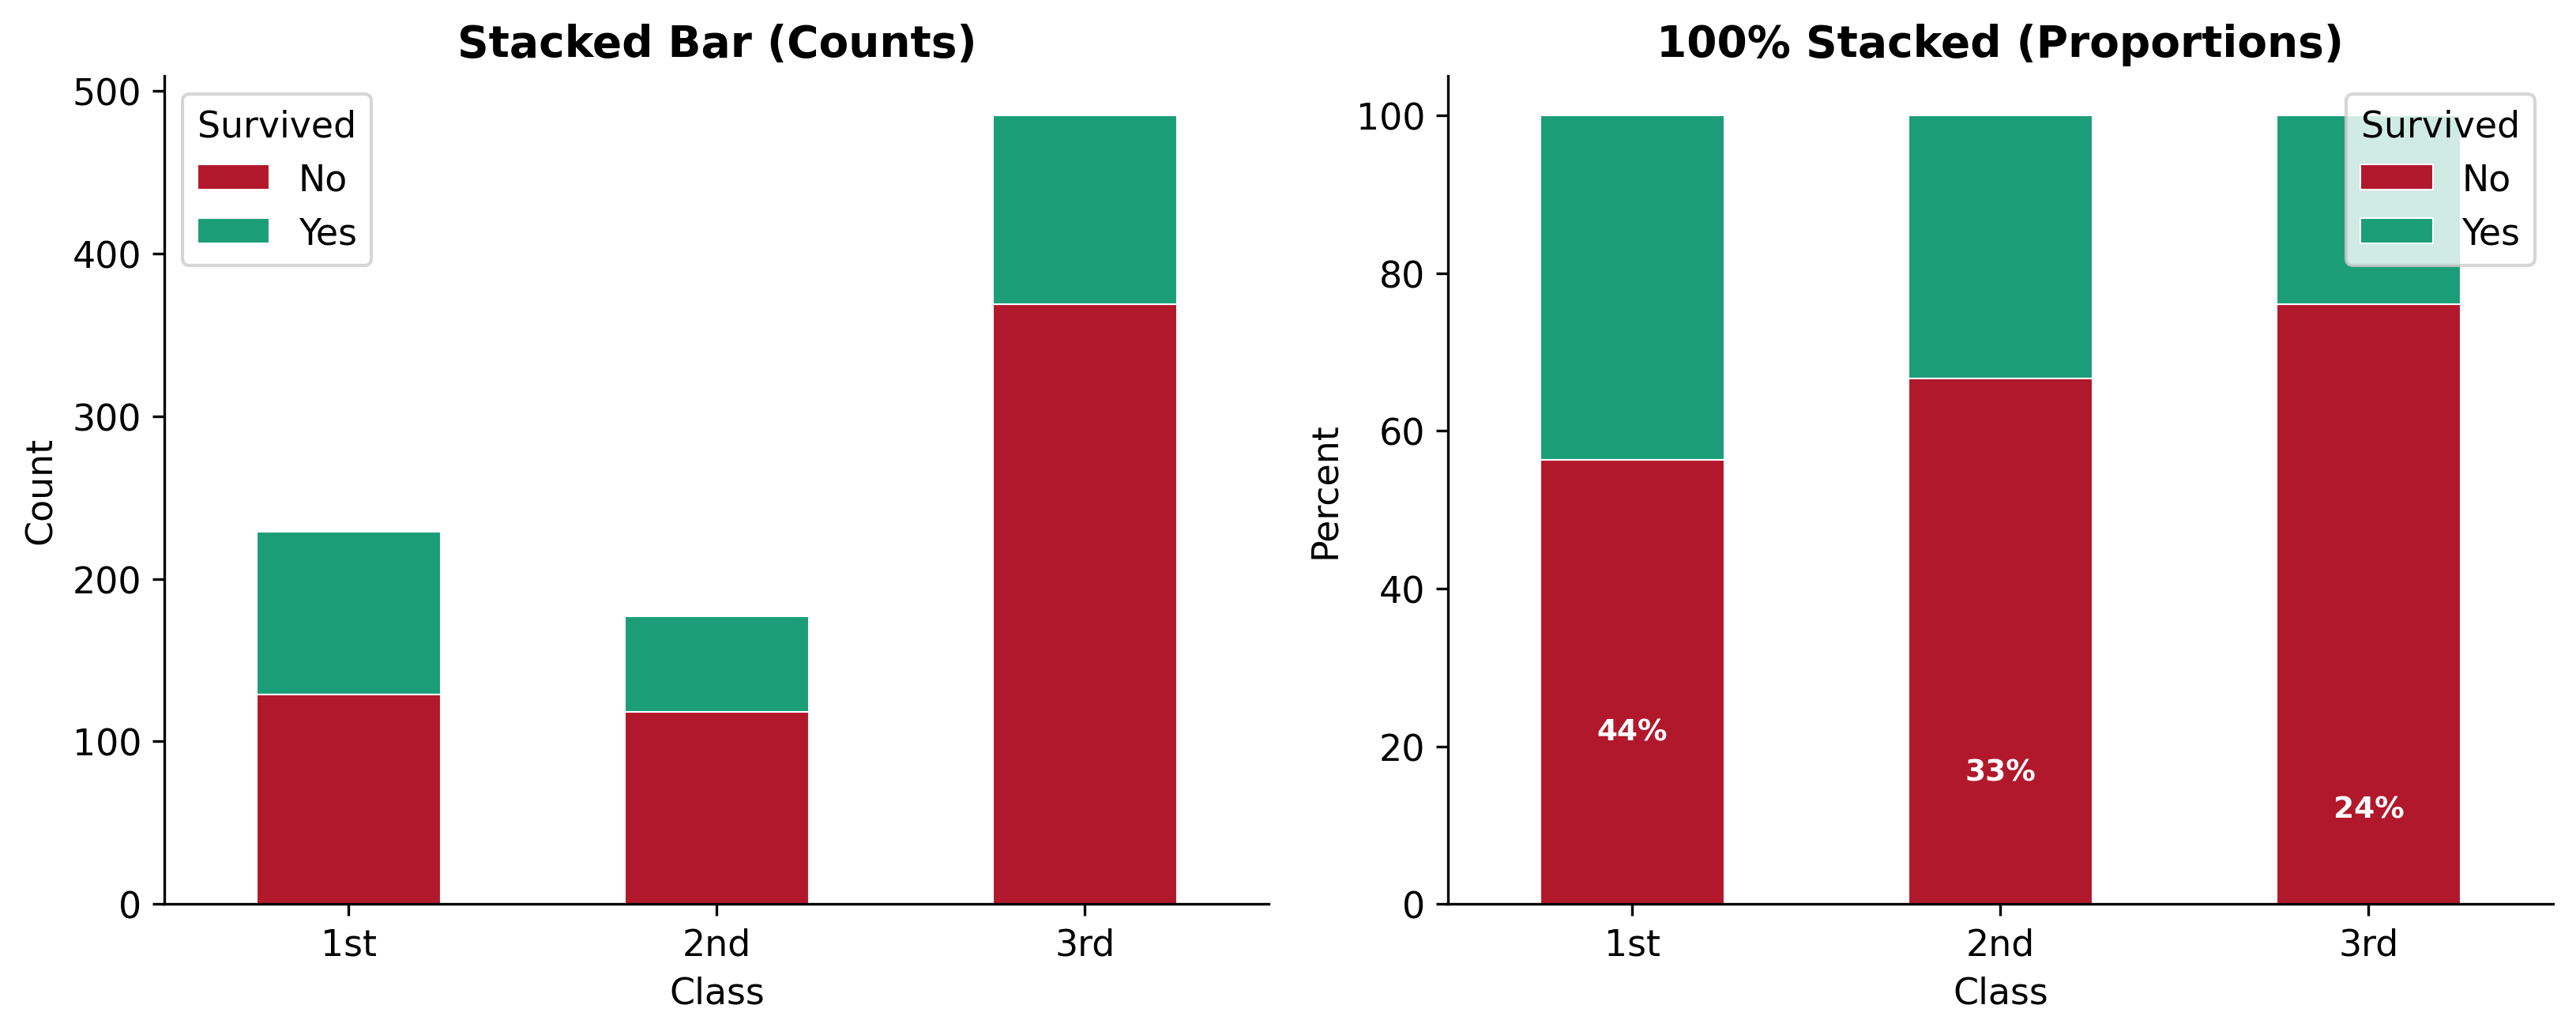
\includegraphics[width=0.88\textwidth]{m3_1_stacked_bar.png}

\vspace{0.2cm}
\begin{columns}[T]
\begin{column}{0.48\textwidth}
\begin{exampleblock}{Data Insight}
    \scriptsize Left: stacked counts show \textbf{total size} per class (3rd is largest) plus composition. Right: 100\% stacked shows \textbf{survival rate} per class (1st had highest). The two answer different questions.
\end{exampleblock}
\end{column}
\begin{column}{0.48\textwidth}
\begin{alertblock}{Pro-Tip}
    \scriptsize Use counts when total size matters (``how many 3rd-class passengers?''). Use proportions when rates matter (``what fraction survived?''). Annotate the percentage inside each segment.
\end{alertblock}
\end{column}
\end{columns}
\end{frame}

% ── 6 ──
\begin{frame}[fragile]{Stacked Bars --- \Rlang}\smark{6/300}
\begin{columns}[T]
\begin{column}{0.55\textwidth}
\begin{lstlisting}[style=Rstyle]
# Counts (default stacked)
ggplot(titanic,
  aes(class, fill=survived)) +
  geom_bar() +
  scale_fill_manual(
    values=c("#B2182B","#1B9E77"))+
  theme_minimal()

# 100% proportions
ggplot(titanic,
  aes(class, fill=survived)) +
  geom_bar(position="fill") +
  scale_y_continuous(
    labels=scales::percent) +
  labs(y="Proportion") +
  theme_minimal()
\end{lstlisting}
\end{column}
\begin{column}{0.42\textwidth}
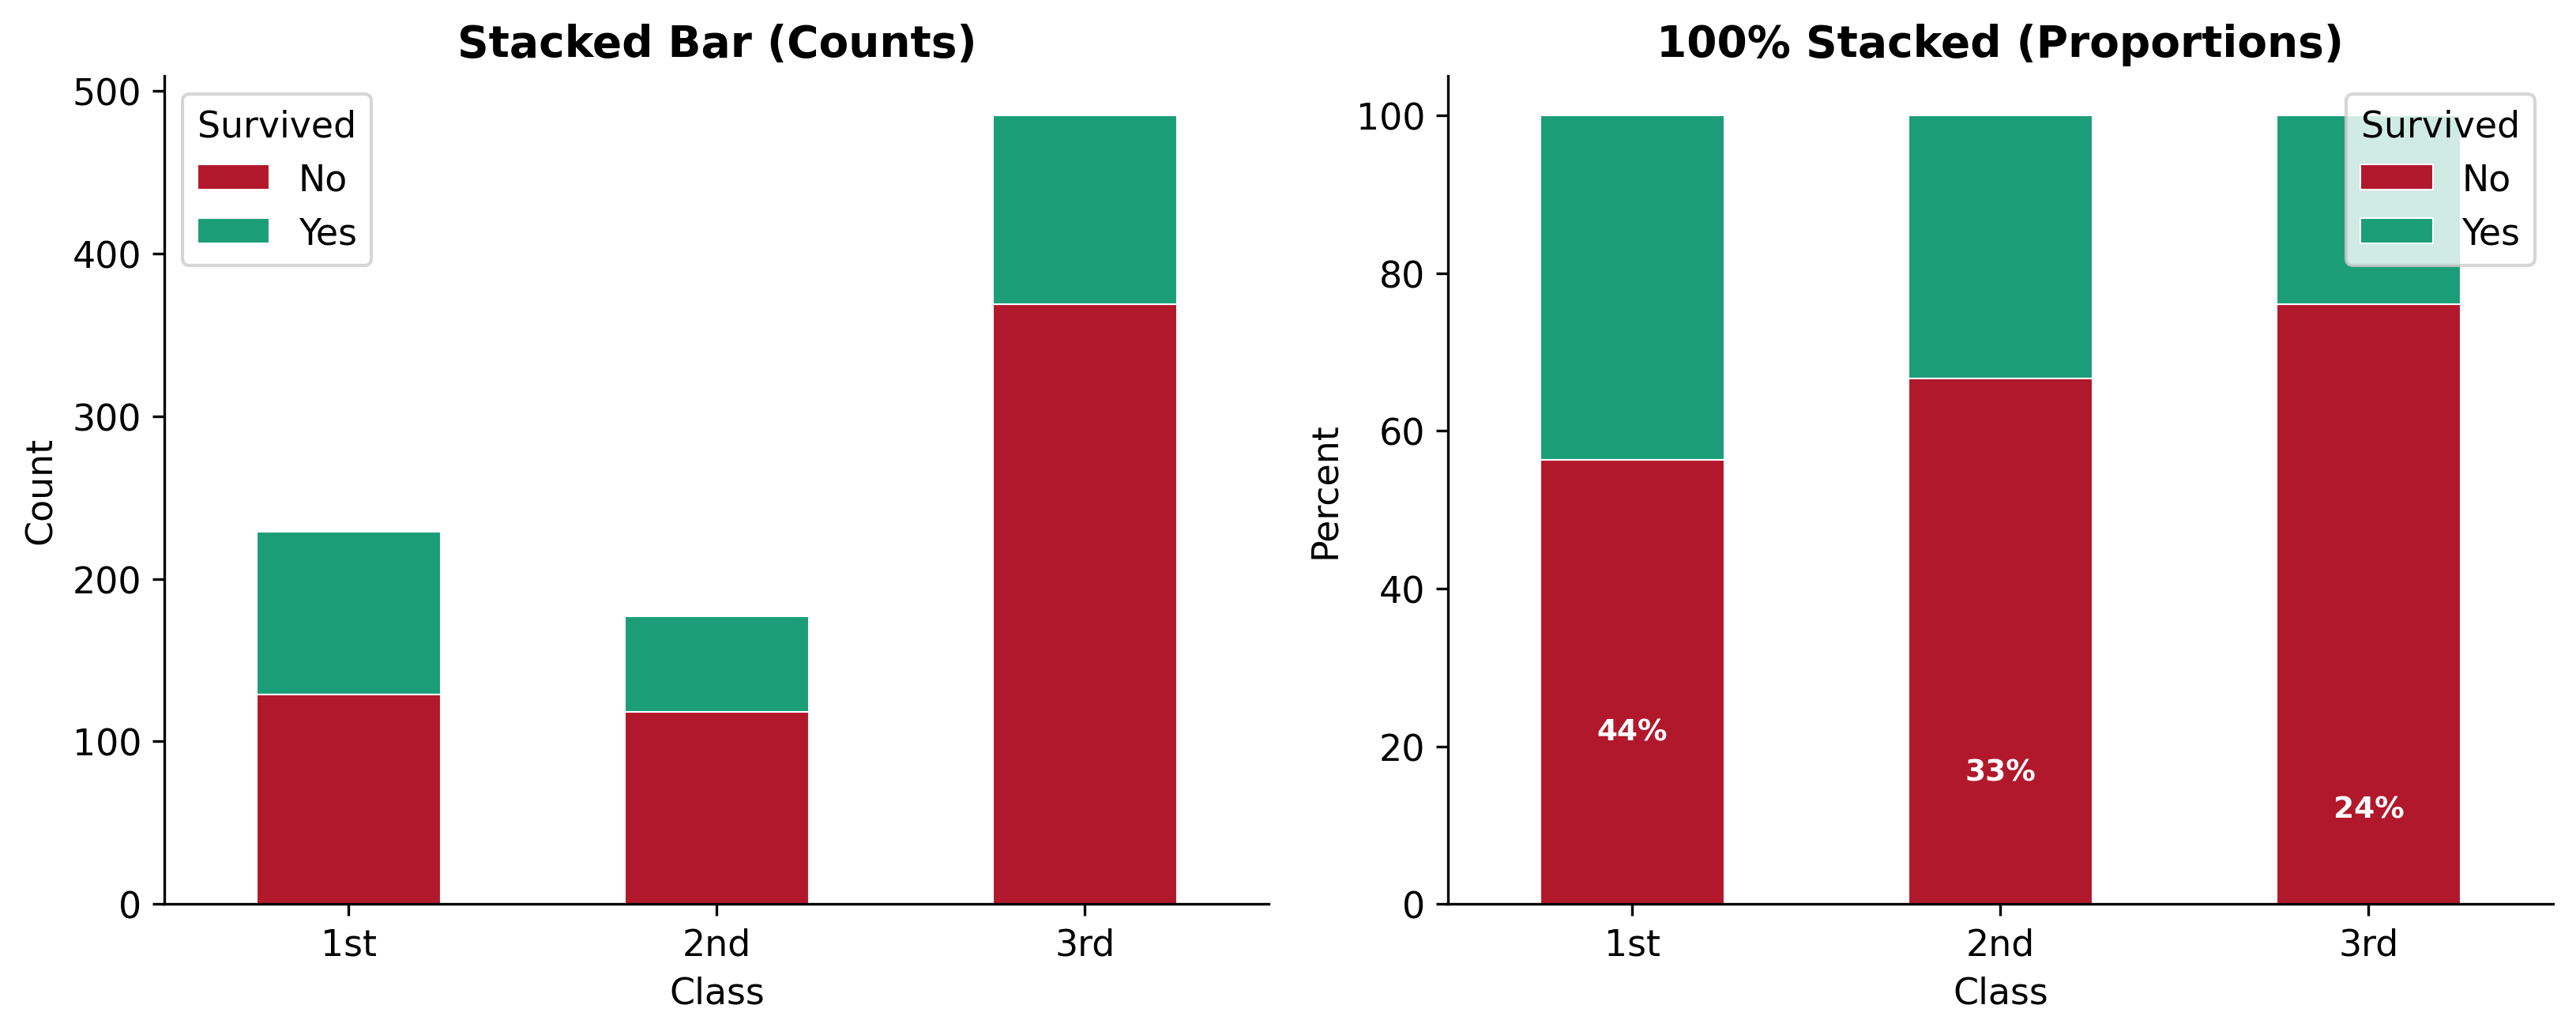
\includegraphics[width=\textwidth]{m3_1_stacked_bar.png}
\begin{alertblock}{Pro-Tip}
    \scriptsize \texttt{position="fill"} normalizes each bar to 100\%. \texttt{position="stack"} (default) preserves counts. \texttt{position="dodge"} places bars side by side.
\end{alertblock}
\end{column}
\end{columns}
\end{frame}

% ── 7 ──
\begin{frame}[fragile]{Stacked Bars --- \Python}\smark{7/300}
\begin{columns}[T]
\begin{column}{0.55\textwidth}
\begin{lstlisting}[style=Pystyle]
# plotnine: stacked
(ggplot(titanic,
   aes("class", fill="survived"))
 + geom_bar(position="stack"))

# plotnine: 100%
(ggplot(titanic,
   aes("class", fill="survived"))
 + geom_bar(position="fill")
 + labs(y="Proportion"))

# seaborn: histplot
sns.histplot(data=titanic,
    x="class", hue="survived",
    multiple="fill", stat="proportion",
    shrink=0.8)

# pandas: manual
ct.div(ct.sum(axis=1), axis=0)\
    .plot(kind="bar", stacked=True)
\end{lstlisting}
\end{column}
\begin{column}{0.42\textwidth}
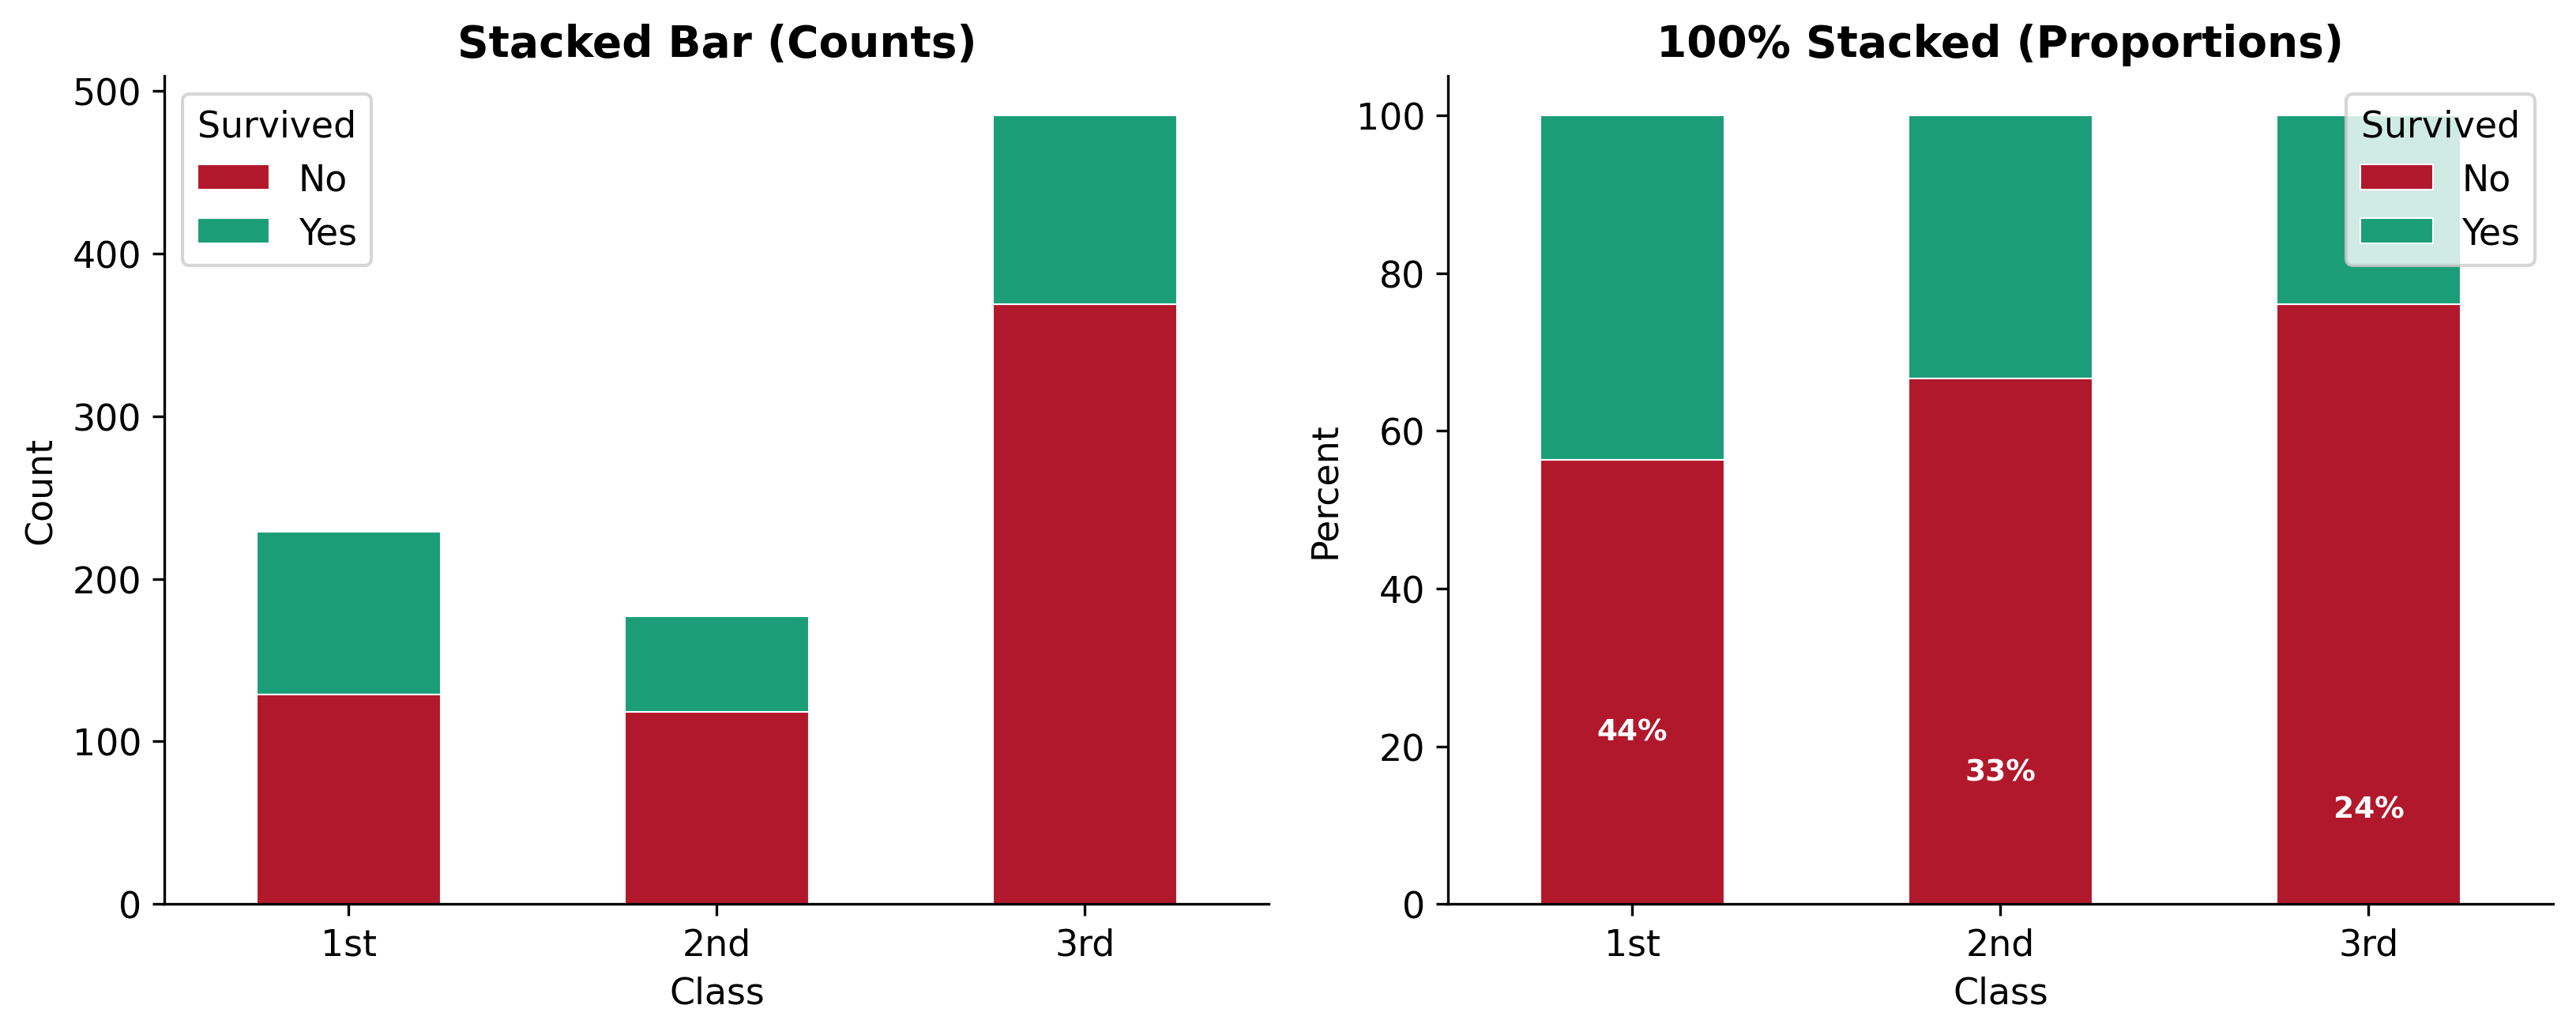
\includegraphics[width=\textwidth]{m3_1_stacked_bar.png}
\begin{exampleblock}{Data Insight}
    \scriptsize seaborn's \texttt{histplot(multiple="fill")} creates 100\% stacked bars. \texttt{multiple="stack"} for counts. \texttt{multiple="dodge"} for grouped.
\end{exampleblock}
\end{column}
\end{columns}
\end{frame}

% ── 8 ──
\begin{frame}{Grouped (Dodged) Bars}
\smark{8/300}
\centering
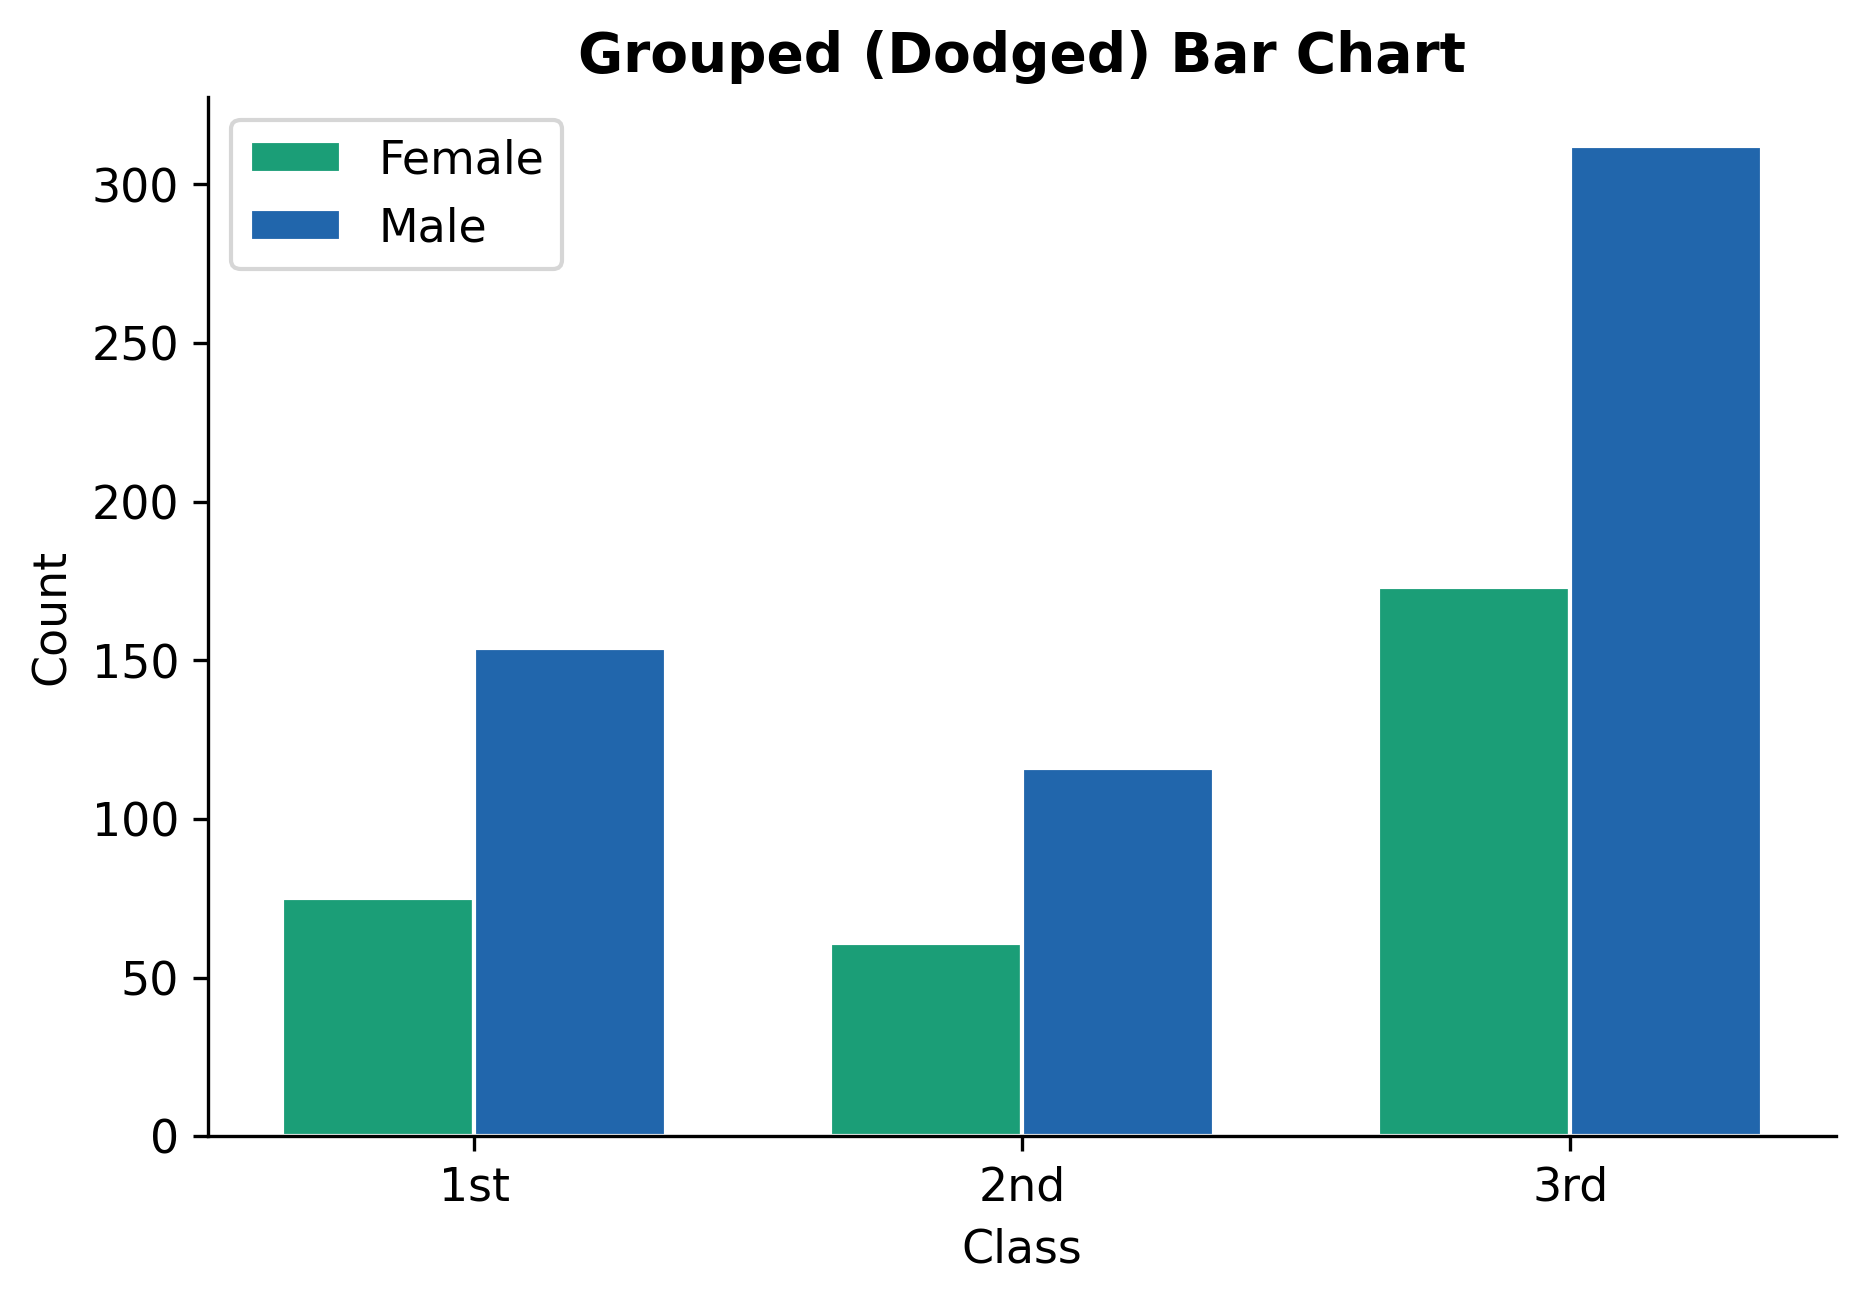
\includegraphics[width=0.65\textwidth]{m3_1_dodged_bar.png}

\vspace{0.2cm}
\begin{columns}[T]
\begin{column}{0.48\textwidth}
\begin{itemize}
    \item Bars placed side by side within each category
    \item Direct comparison of sub-groups
    \item Better than stacked for \textbf{exact} value comparison
    \item Worse than stacked for \textbf{total} and \textbf{composition}
\end{itemize}
\end{column}
\begin{column}{0.48\textwidth}
\begin{alertblock}{Pro-Tip}
    \scriptsize Use dodged bars for $\leq 3$ sub-groups. Beyond 3, the bars become too narrow. Switch to faceted bars or a Cleveland dot plot for 4+ sub-groups.
\end{alertblock}
\end{column}
\end{columns}
\end{frame}

% ── 9 ──
\begin{frame}[fragile]{Dodged Bars --- Code}\smark{9/300}
\begin{columns}[T]
\begin{column}{0.48\textwidth}
\begin{lstlisting}[style=Rstyle]
ggplot(titanic,
  aes(class, fill = sex)) +
  geom_bar(position = "dodge") +
  scale_fill_manual(
    values=c("#1B9E77","#2166AC"))+
  theme_minimal()

# With counts on top
ggplot(titanic,
  aes(class, fill = sex)) +
  geom_bar(position =
    position_dodge(width=0.9)) +
  geom_text(stat="count",
    aes(label=after_stat(count)),
    position=position_dodge(0.9),
    vjust=-0.5, size=3) +
  theme_minimal()
\end{lstlisting}
\end{column}
\begin{column}{0.48\textwidth}
\begin{lstlisting}[style=Pystyle]
# seaborn
sns.countplot(data=titanic,
    x="class", hue="sex",
    palette=["#1B9E77","#2166AC"])

# plotnine
(ggplot(titanic,
   aes("class", fill="sex"))
 + geom_bar(position="dodge"))

# matplotlib manual
x = np.arange(3)
w = 0.35
ax.bar(x-w/2, female_counts, w,
    label="Female")
ax.bar(x+w/2, male_counts, w,
    label="Male")
\end{lstlisting}
\end{column}
\end{columns}
\end{frame}

% ── 10 ──
\begin{frame}{Stacked vs.\ Dodged vs.\ Faceted: Decision Guide}
\smark{10/300}
\centering\small
\begin{tabular}{@{}lllll@{}}
    \toprule
    \textbf{Layout} & \textbf{Compare} & \textbf{Total?} & \textbf{Sub-groups} & \textbf{Best When} \\
    \midrule
    Stacked   & Composition & Yes    & 2--4   & Part-of-whole + total \\
    100\% fill& Proportions & No     & 2--4   & Rate comparison \\
    Dodged    & Values      & No     & 2--3   & Exact sub-group comparison \\
    Faceted   & All         & Per panel& Any  & Many sub-groups ($>3$) \\
    \bottomrule
\end{tabular}

\vspace{0.3cm}
\begin{exampleblock}{Data Insight}
    \scriptsize The middle segments of stacked bars (not the top or bottom) are hardest to compare because they have no common baseline. Dodged bars fix this but sacrifice the whole-part view.
\end{exampleblock}
\end{frame}

% ── 11 ──
\begin{frame}{Mosaic Plots: The 2D Proportional Display}
\smark{11/300}
\centering
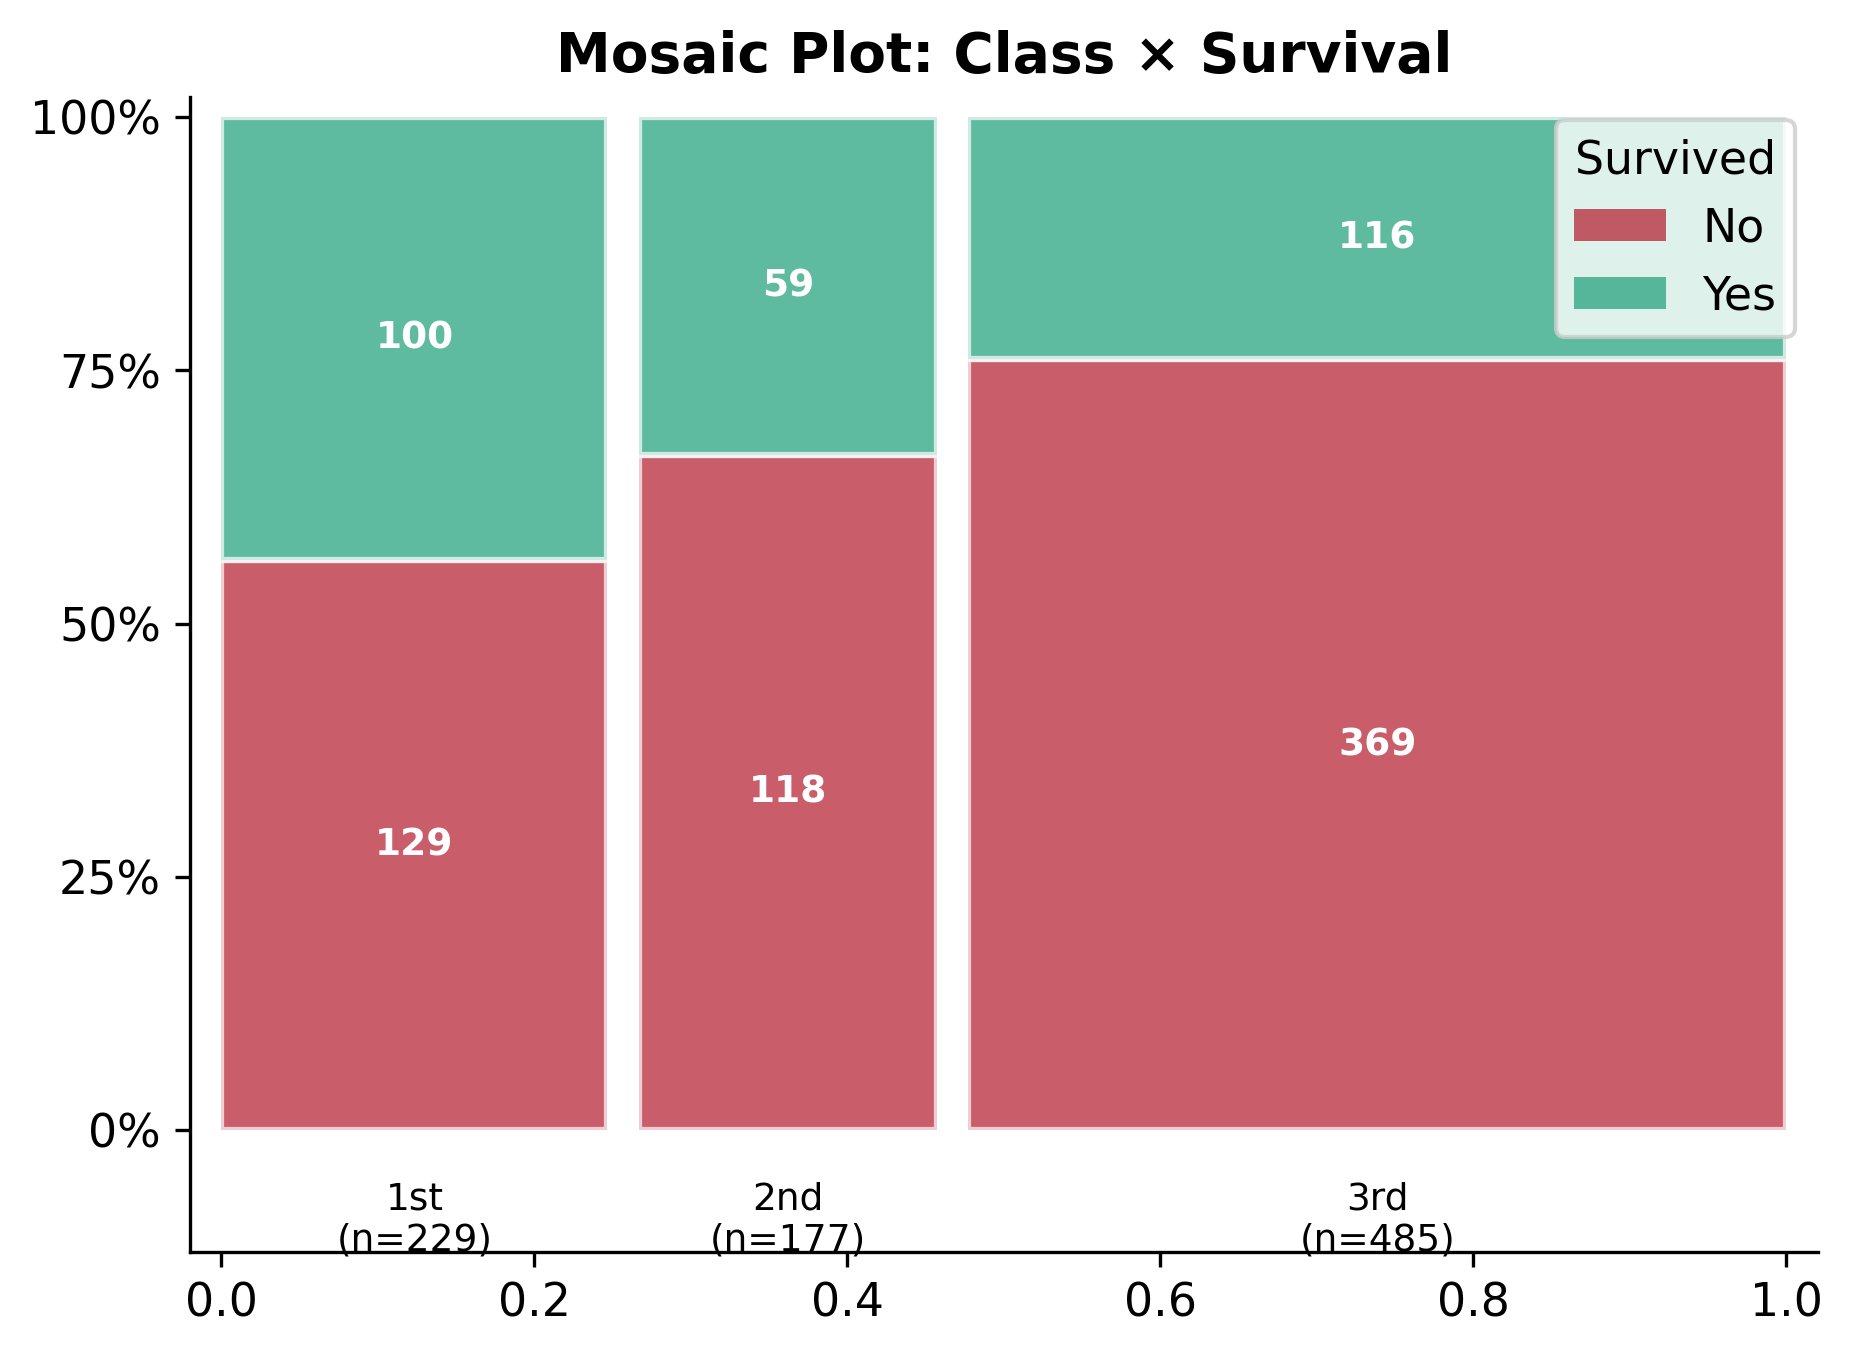
\includegraphics[width=0.62\textwidth]{m3_1_mosaic.png}

\vspace{0.2cm}
\begin{columns}[T]
\begin{column}{0.48\textwidth}
\begin{itemize}
    \item Width $\propto$ column marginal (class size)
    \item Height $\propto$ conditional proportion (survival rate within class)
    \item Area $\propto$ joint frequency (cell count)
    \item Encodes \textbf{three} things: marginals, conditionals, and joint
\end{itemize}
\end{column}
\begin{column}{0.48\textwidth}
\begin{exampleblock}{Data Insight}
    \scriptsize 3rd class is widest (most passengers) but mostly red (lowest survival). 1st class is narrower but mostly green. The mosaic plot reveals both the size imbalance and the survival disparity simultaneously.
\end{exampleblock}
\end{column}
\end{columns}
\end{frame}

% ── 12 ──
\begin{frame}[fragile]{Mosaic Plot --- \Rlang}\smark{12/300}
\begin{columns}[T]
\begin{column}{0.55\textwidth}
\begin{lstlisting}[style=Rstyle]
# vcd package (Friendly)
library(vcd)
mosaic(survived ~ class,
  data = titanic,
  shade = TRUE,
  legend = TRUE)

# ggmosaic (ggplot2-based)
library(ggmosaic)
ggplot(titanic) +
  geom_mosaic(aes(
    x = product(survived, class),
    fill = survived)) +
  scale_fill_manual(
    values=c("#B2182B","#1B9E77"))+
  theme_minimal()
\end{lstlisting}
\end{column}
\begin{column}{0.42\textwidth}
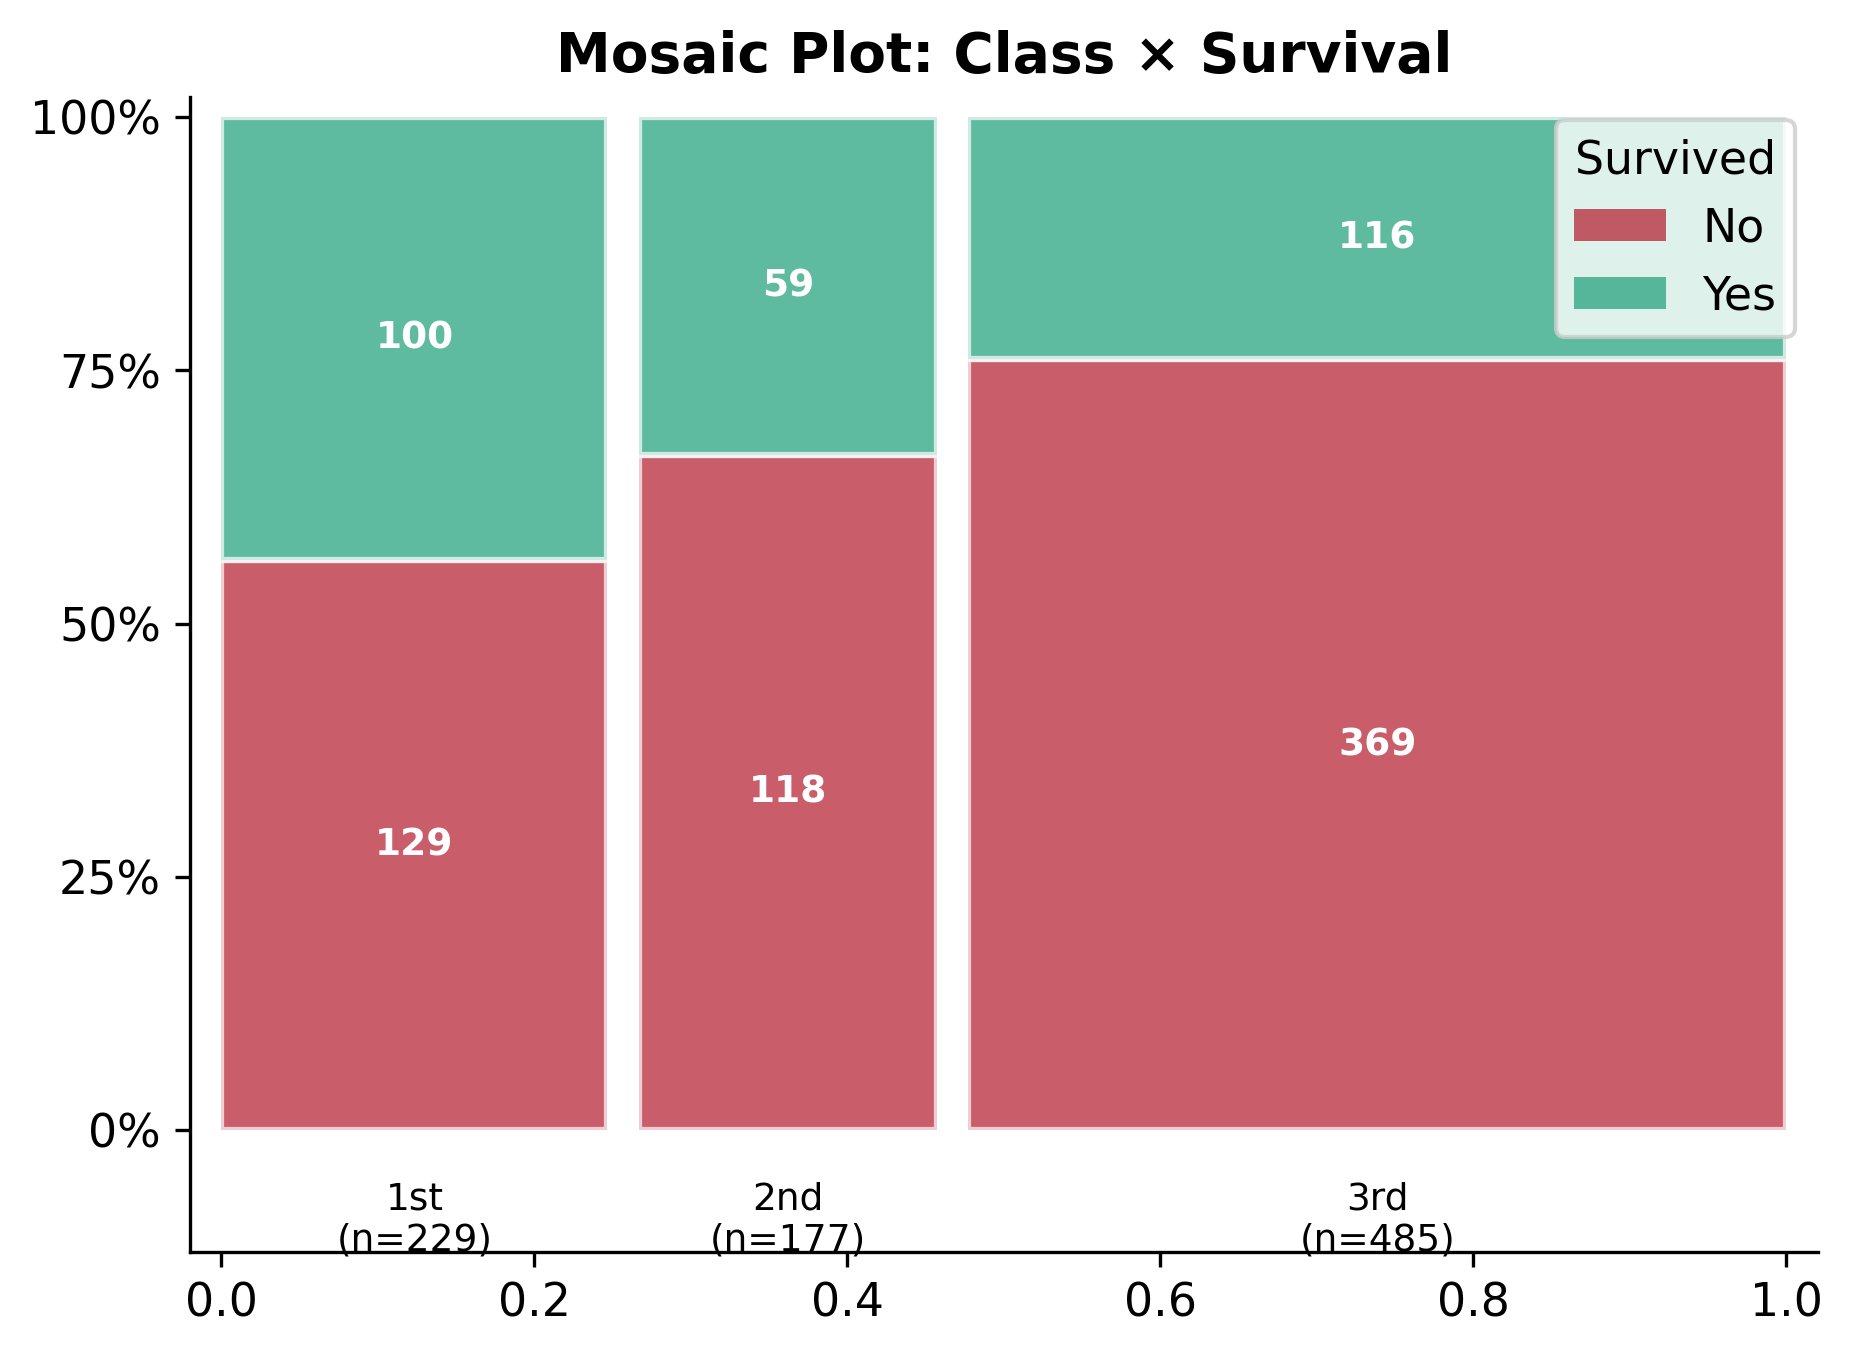
\includegraphics[width=\textwidth]{m3_1_mosaic.png}
\begin{alertblock}{Pro-Tip}
    \scriptsize \texttt{vcd::mosaic(shade=TRUE)} colors cells by Pearson residuals: blue = more than expected, red = fewer. This adds the $\chi^2$ test interpretation directly to the display.
\end{alertblock}
\end{column}
\end{columns}
\end{frame}

% ── 13 ──
\begin{frame}[fragile]{Mosaic Plot --- \Python}\smark{13/300}
\begin{columns}[T]
\begin{column}{0.55\textwidth}
\begin{lstlisting}[style=Pystyle]
# statsmodels mosaic
from statsmodels.graphics.mosaicplot\
    import mosaic

fig, ax = plt.subplots(figsize=(7,5))
mosaic(titanic,
    ["class","survived"],
    ax=ax,
    properties=lambda key:
        {"color": "#1B9E77"
         if "Yes" in key
         else "#B2182B"})

# plotnine: no native mosaic.
# Use geom_tile() on pre-computed
# proportions with variable widths.
# The vcd R package remains the
# gold standard for mosaic plots.
\end{lstlisting}
\end{column}
\begin{column}{0.42\textwidth}
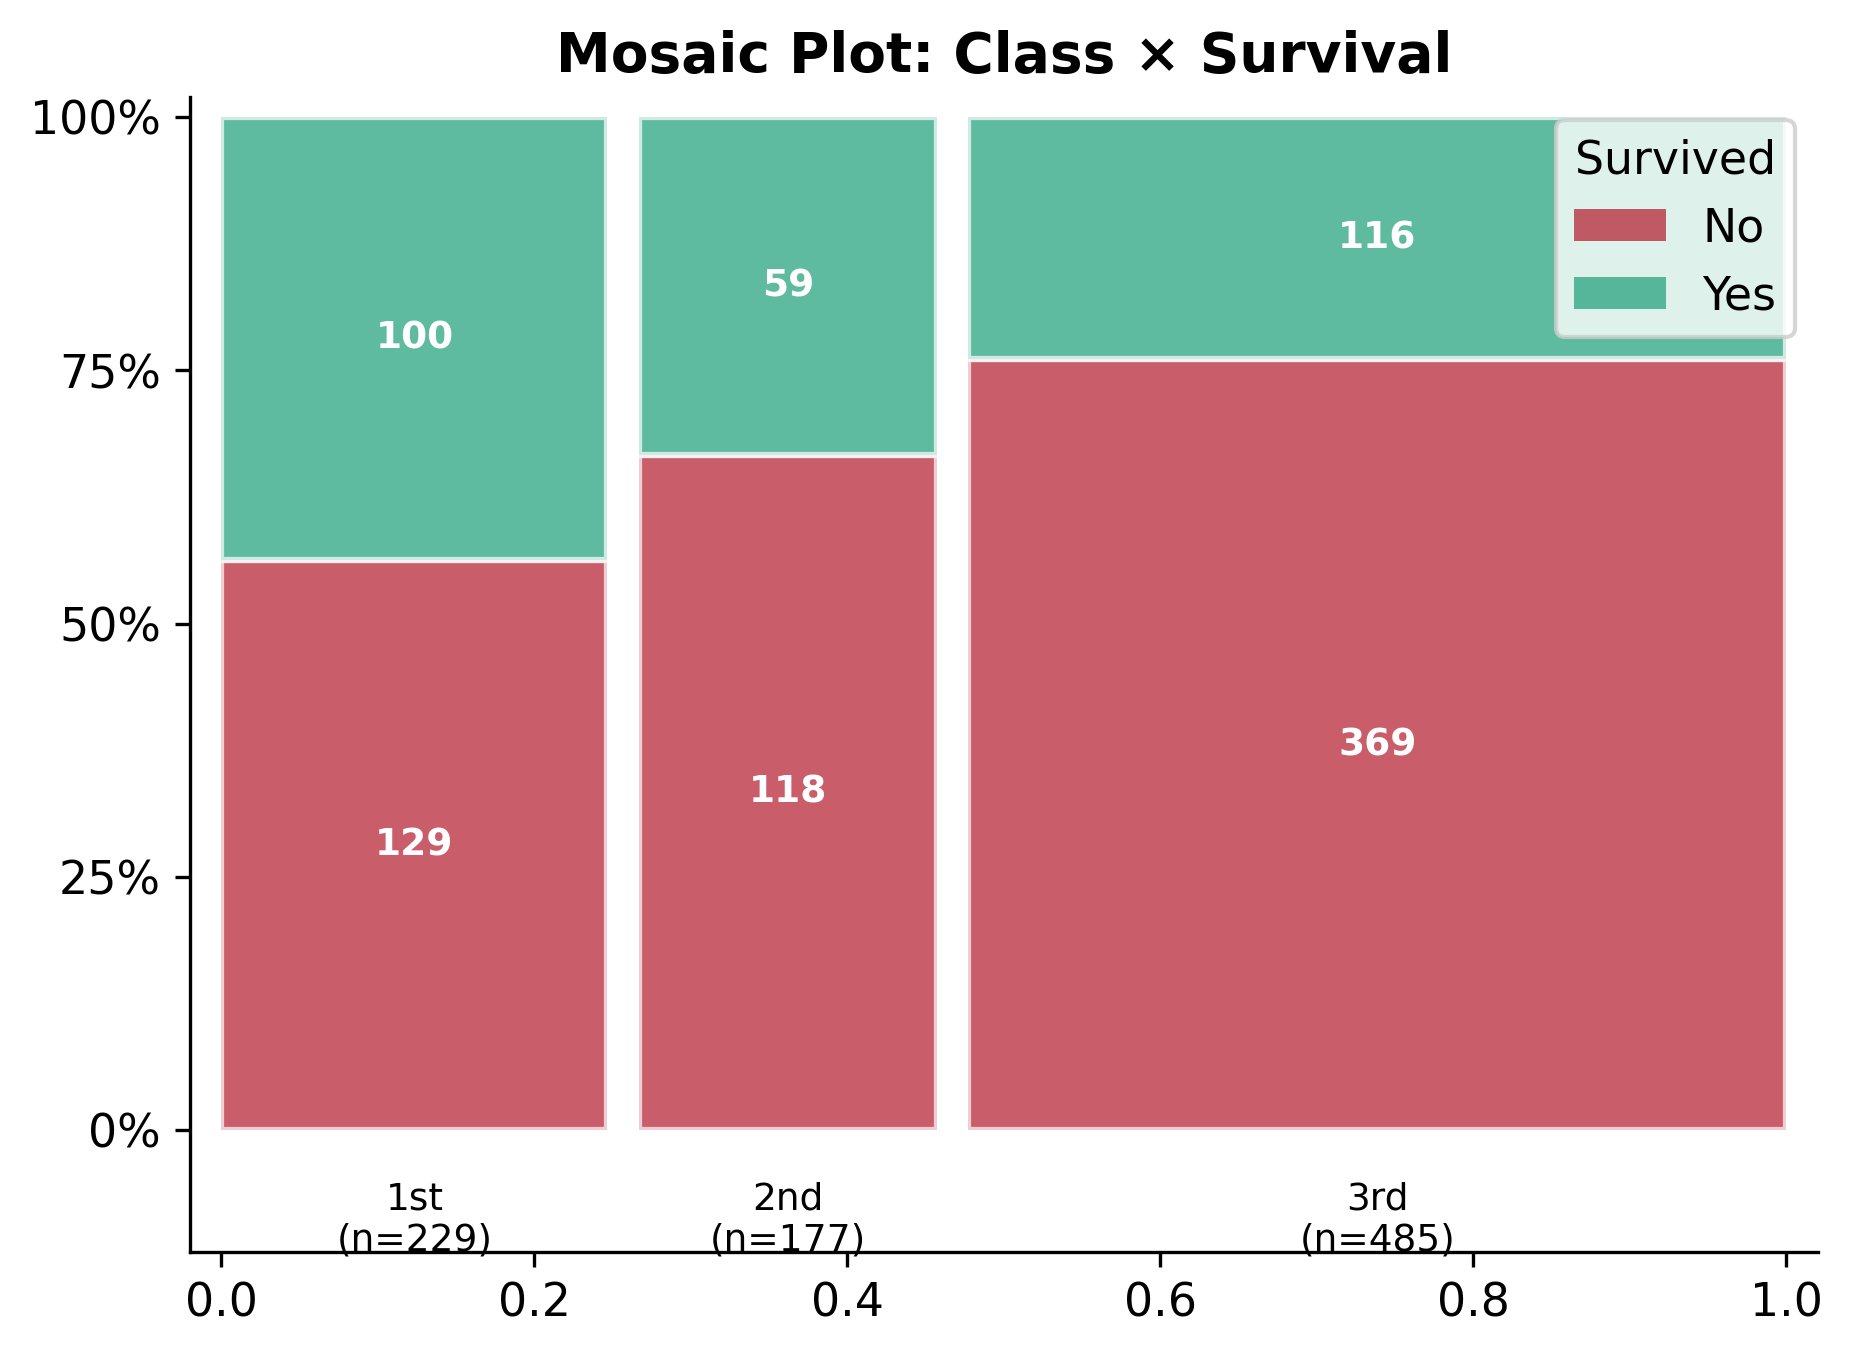
\includegraphics[width=\textwidth]{m3_1_mosaic.png}
\begin{exampleblock}{Data Insight}
    \scriptsize Python's mosaic plot support is limited. \texttt{statsmodels.graphics.mosaicplot.mosaic()} works but lacks shading by residual. For publication-quality mosaics, R's \texttt{vcd} package is superior.
\end{exampleblock}
\end{column}
\end{columns}
\end{frame}

% ── 14 ──
\begin{frame}{Spine Plots: 1D Proportional Bars}
\smark{14/300}
\centering
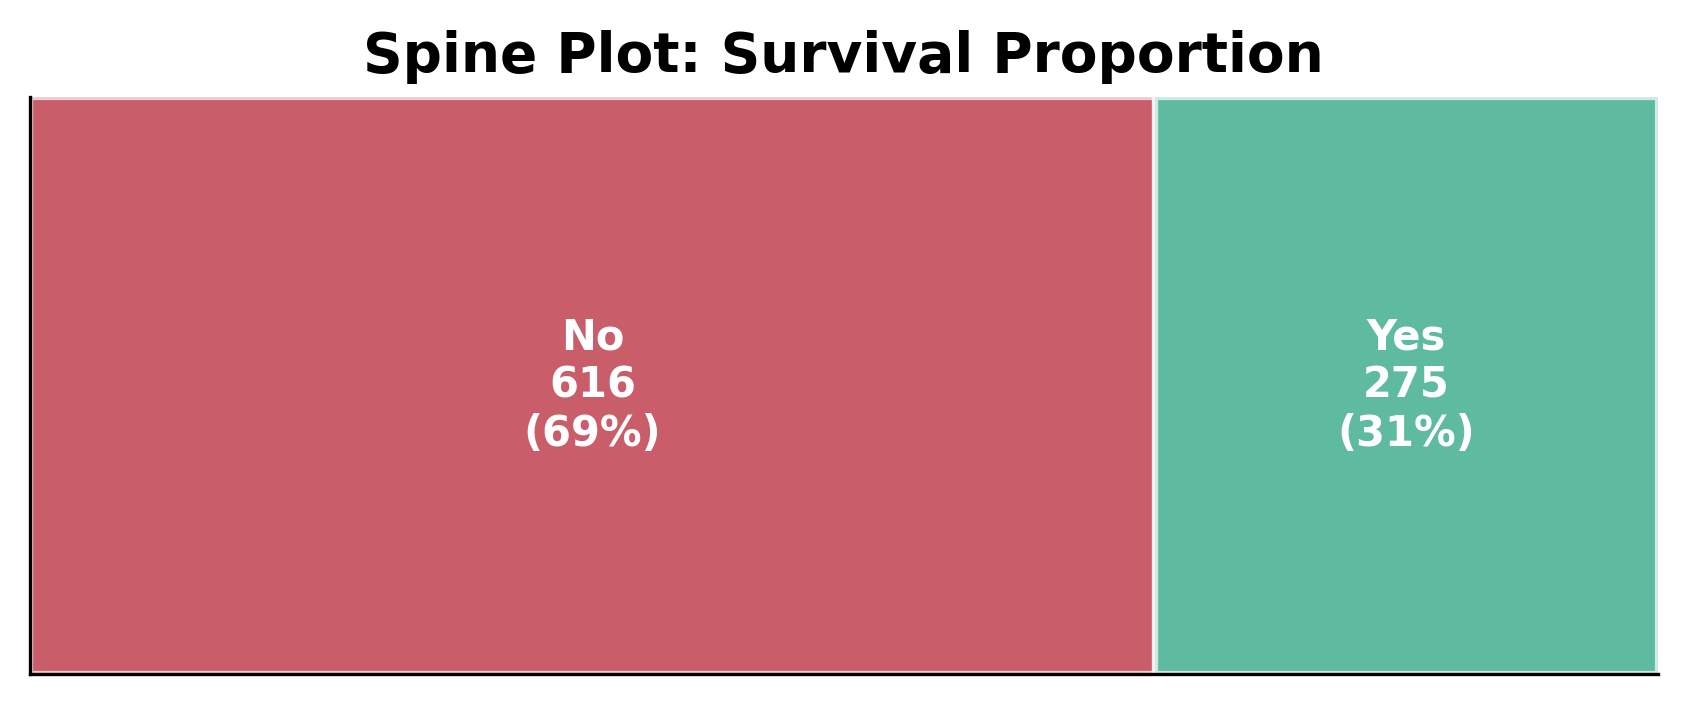
\includegraphics[width=0.78\textwidth]{m3_1_spine.png}

\vspace{0.2cm}
\begin{columns}[T]
\begin{column}{0.48\textwidth}
\begin{itemize}
    \item A single bar spanning the full width
    \item Segments proportional to category counts
    \item The simplest part-of-whole display
    \item Better than pie for 2--4 categories (position encoding vs.\ angle)
\end{itemize}
\end{column}
\begin{column}{0.48\textwidth}
\begin{alertblock}{Pro-Tip}
    \scriptsize Spine plots are the 1D analog of mosaic plots. A mosaic is a spine plot \textbf{conditioned} on a second variable. Both use area proportional to frequency.
\end{alertblock}
\end{column}
\end{columns}
\end{frame}

% ── 15 ──
\begin{frame}[fragile]{Spine Plot --- Code}\smark{15/300}
\begin{columns}[T]
\begin{column}{0.48\textwidth}
\begin{lstlisting}[style=Rstyle]
# vcd::spine (base R plot)
library(vcd)
spine(survived ~ class,
      data = titanic)

# ggplot2: geom_bar(position="fill")
# rotated is a spine plot
ggplot(titanic,
  aes(x = 1, fill = survived)) +
  geom_bar(position = "fill",
    width = 1) +
  coord_flip() +
  scale_fill_manual(
    values=c("#B2182B","#1B9E77"))+
  theme_void()
\end{lstlisting}
\end{column}
\begin{column}{0.48\textwidth}
\begin{lstlisting}[style=Pystyle]
# Manual with matplotlib
counts = titanic["survived"]\
    .value_counts()
total = counts.sum()
x_start = 0
for label, c in [("No","#B2182B"),
                  ("Yes","#1B9E77")]:
    w = counts[label] / total
    ax.barh(0, w, left=x_start,
        color=c, height=0.6)
    ax.text(x_start+w/2, 0,
        f"{label}\n{w:.0%}",
        ha="center", va="center",
        color="white", fontweight="bold")
    x_start += w
ax.set_xlim(0, 1)
ax.set_yticks([])
\end{lstlisting}
\end{column}
\end{columns}
\end{frame}

% ── 16 ──
\begin{frame}{Waffle Charts: Discrete Part-of-Whole}
\smark{16/300}
\centering
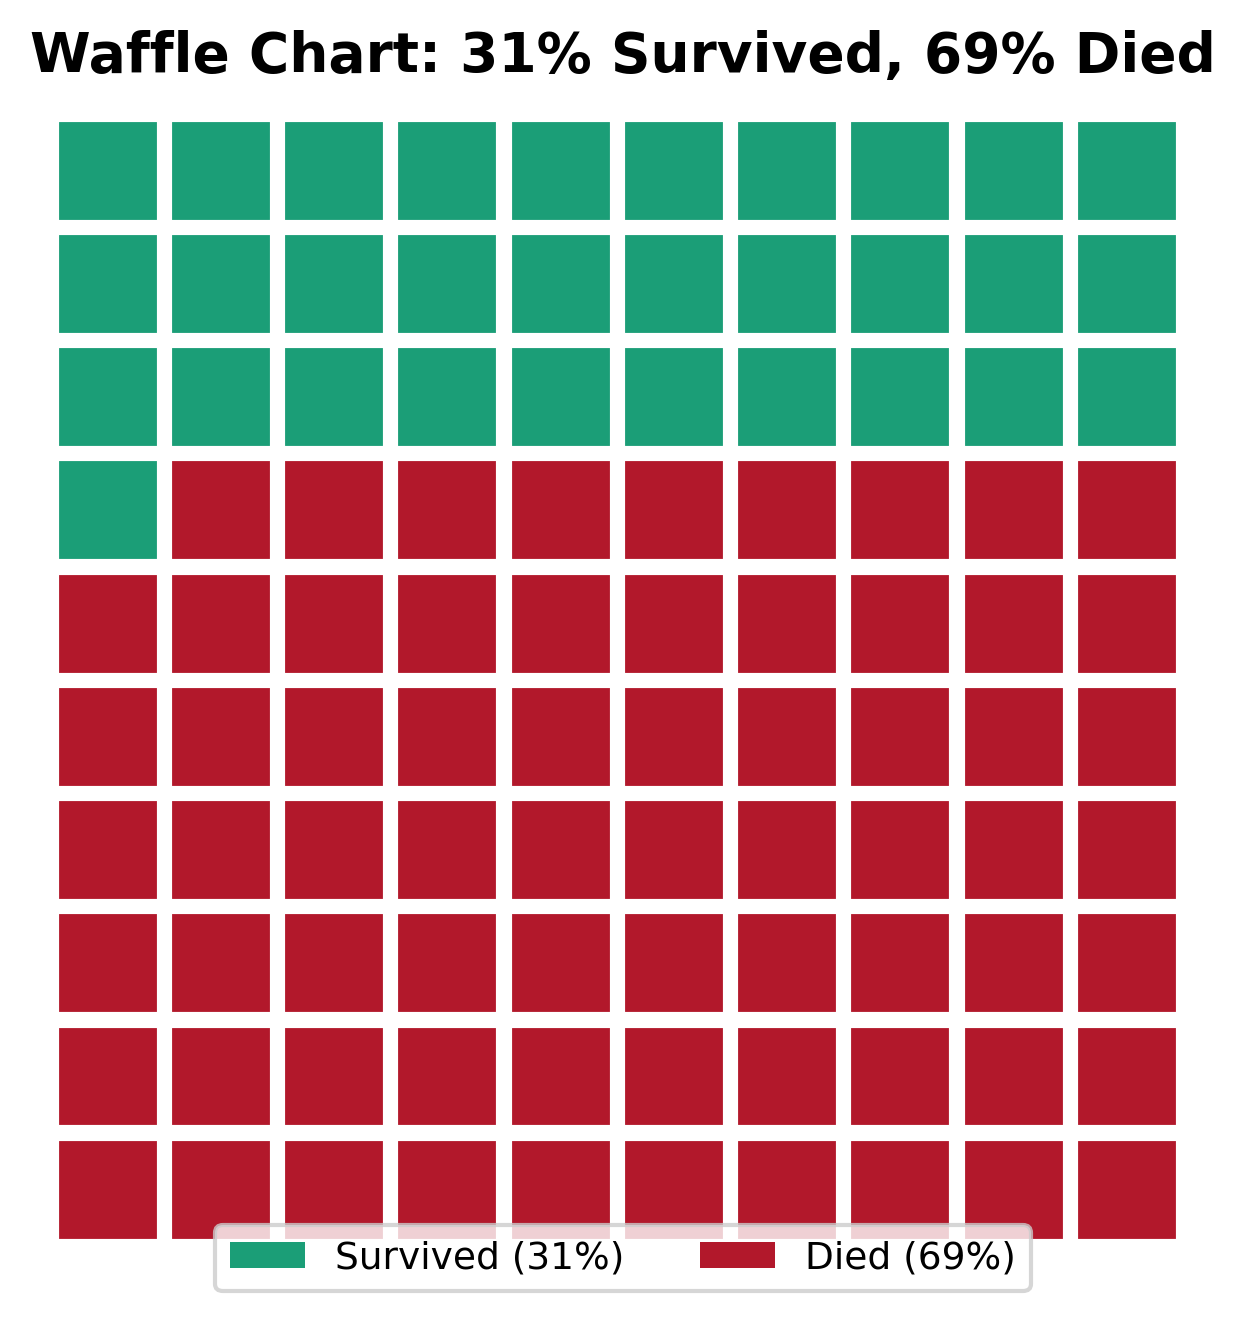
\includegraphics[width=0.55\textwidth]{m3_1_waffle.png}

\vspace{0.2cm}
\begin{columns}[T]
\begin{column}{0.48\textwidth}
\begin{itemize}
    \item $10 \times 10$ grid = 100 squares
    \item Each square = 1\% of the total
    \item Readers can \textbf{count} squares for exact proportion
    \item Much more accurate than pie charts for small differences
\end{itemize}
\end{column}
\begin{column}{0.48\textwidth}
\begin{exampleblock}{Data Insight}
    \scriptsize Waffle charts outperform pie charts because they use \textbf{position and counting} (high accuracy) instead of \textbf{angle} (low accuracy). The grid makes ``31\% vs.\ 34\%'' distinguishable; a pie cannot.
\end{exampleblock}
\end{column}
\end{columns}
\end{frame}

% ── 17 ──
\begin{frame}[fragile]{Waffle Chart --- Code}\smark{17/300}
\begin{columns}[T]
\begin{column}{0.48\textwidth}
\begin{lstlisting}[style=Rstyle]
library(waffle)

vals <- c(Survived=31, Died=69)
waffle(vals, rows=10, size=0.5,
  colors=c("#1B9E77","#B2182B"),
  title="Survival Rate") +
  theme_void()

# Iron waffle (pictogram)
iron(waffle(vals, rows=10,
  colors=c("#1B9E77","#B2182B")))

# ggwaffle alternative
library(ggwaffle)
ggplot(waffle_df, aes(x, y,
    fill=group)) +
  geom_waffle() + coord_equal() +
  theme_void()
\end{lstlisting}
\end{column}
\begin{column}{0.48\textwidth}
\begin{lstlisting}[style=Pystyle]
# pip install pywaffle
from pywaffle import Waffle

fig = plt.figure(
    FigureClass=Waffle,
    rows=10, columns=10,
    values=[31, 69],
    colors=["#1B9E77","#B2182B"],
    labels=["Survived","Died"],
    legend={"loc":"lower center",
            "ncol":2})
fig.suptitle("Survival Rate")

# Manual: matplotlib patches
for row in range(10):
    for col in range(10):
        c = colors[idx]
        ax.add_patch(Rectangle(
            (col, 9-row), 0.9, 0.9,
            facecolor=c))
\end{lstlisting}
\end{column}
\end{columns}
\end{frame}

% ── 18 ──
\begin{frame}{Pie Charts: When (Rarely) to Use Them}
\smark{18/300}
\begin{columns}[T]
\begin{column}{0.50\textwidth}
\begin{itemize}
    \item Encode proportions as \textbf{angle} (rank 4, Cleveland)
    \item Humans are poor at judging angles accurately
    \item Only acceptable for \textbf{2--3 slices} where the difference is large
    \item \textbf{Never} for 5+ categories
    \item \textbf{Never} for exact comparison tasks
\end{itemize}
\end{column}
\begin{column}{0.47\textwidth}
\begin{alertblock}{Pro-Tip}
    \scriptsize If a reviewer or stakeholder insists on a pie chart, use a \textbf{donut chart} (hollow center) with direct percentage labels. The labels carry the information; the chart is decorative.
\end{alertblock}
\vspace{0.1cm}
\begin{exampleblock}{Data Insight}
    \scriptsize ``No one has ever made a pie chart more informative by making it 3D.'' Avoid 3D pie charts under all circumstances --- they distort angles through perspective projection.
\end{exampleblock}
\end{column}
\end{columns}
\end{frame}

% ── 19 ──
\begin{frame}[fragile]{Pie and Donut --- Code}\smark{19/300}
\begin{columns}[T]
\begin{column}{0.48\textwidth}
\begin{lstlisting}[style=Rstyle]
# Pie (if you must)
ggplot(df, aes(x="", y=n,
    fill=category)) +
  geom_col(width=1) +
  coord_polar("y") +
  theme_void()

# Donut (slightly better)
ggplot(df, aes(x=2, y=n,
    fill=category)) +
  geom_col(width=1) +
  coord_polar("y") +
  xlim(0.5, 2.5) + # hollow center
  theme_void()
\end{lstlisting}
\end{column}
\begin{column}{0.48\textwidth}
\begin{lstlisting}[style=Pystyle]
# Pie
ax.pie(values, labels=labels,
    autopct="%1.0f%%",
    colors=["#1B9E77","#B2182B"])

# Donut
wedges, texts, autotexts = ax.pie(
    values, labels=labels,
    autopct="%1.0f%%",
    pctdistance=0.75)
centre = plt.Circle((0,0), 0.5,
    fc="white")
ax.add_artist(centre)
\end{lstlisting}
\vspace{0.1cm}
\begin{alertblock}{Pro-Tip}
    \scriptsize In the grammar: pie = \texttt{geom\_col(width=1) + coord\_polar("y")}. Understanding this decomposition makes it clear why a pie is just a transformed bar --- and usually a worse one.
\end{alertblock}
\end{column}
\end{columns}
\end{frame}

% ── 20 ──
\begin{frame}{Lollipop Charts: Dot + Stem}
\smark{20/300}
\centering
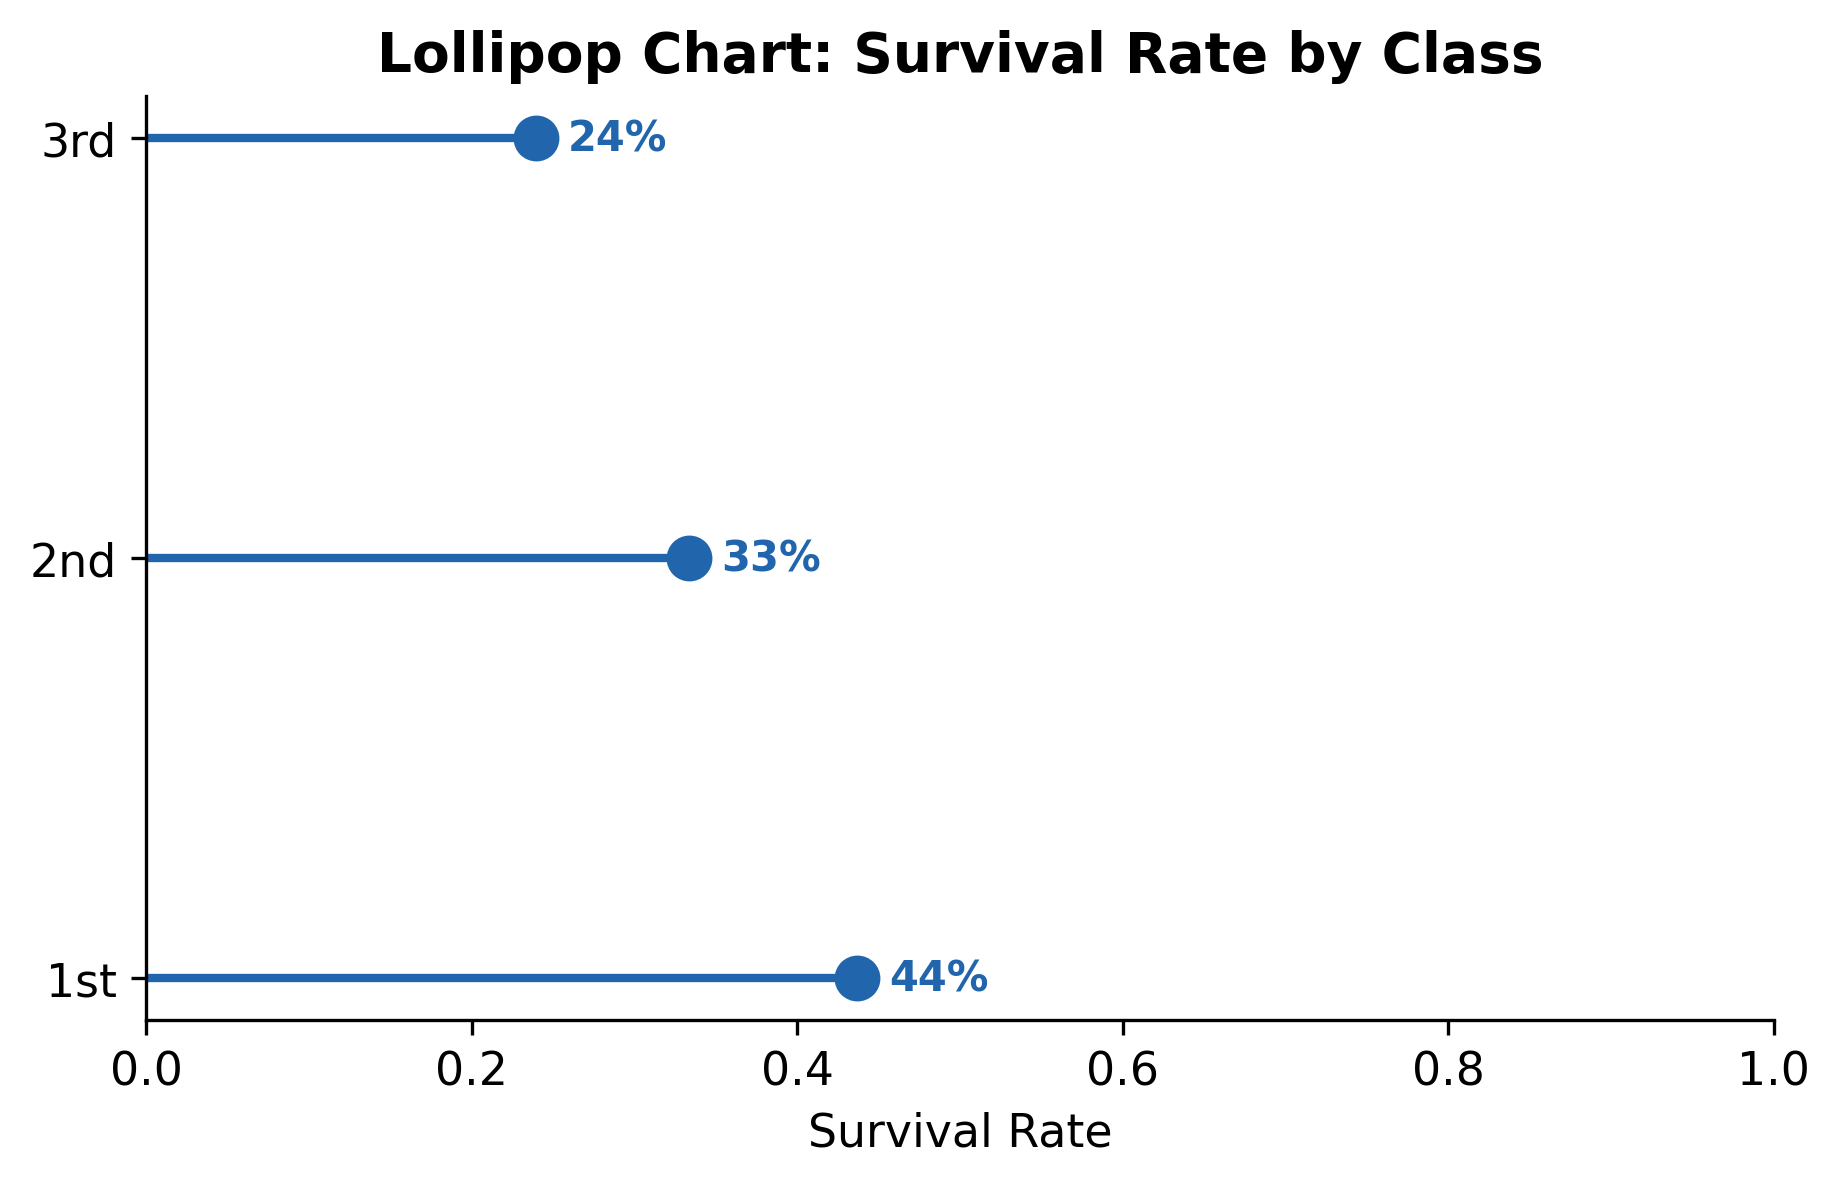
\includegraphics[width=0.68\textwidth]{m3_1_lollipop.png}

\vspace{0.2cm}
\begin{columns}[T]
\begin{column}{0.48\textwidth}
\begin{itemize}
    \item A dot at the value, connected to the baseline by a thin line
    \item Less ink than a bar; same position encoding
    \item Especially good for \textbf{rates and proportions} where zero-baseline is important
    \item Works horizontally for long labels
\end{itemize}
\end{column}
\begin{column}{0.48\textwidth}
\begin{exampleblock}{Data Insight}
    \scriptsize Lollipop charts are the ``light'' version of bar charts. They preserve the baseline anchor (unlike Cleveland dot plots) while reducing visual weight. Ideal for dashboards.
\end{exampleblock}
\end{column}
\end{columns}
\end{frame}

% ── 21 ──
\begin{frame}[fragile]{Lollipop --- Code}\smark{21/300}
\begin{columns}[T]
\begin{column}{0.48\textwidth}
\begin{lstlisting}[style=Rstyle]
ggplot(surv_df,
  aes(fct_reorder(class, rate),
      rate)) +
  geom_segment(aes(
    xend=class, y=0, yend=rate),
    color="#2166AC", linewidth=1) +
  geom_point(color="#2166AC",
    size=4) +
  coord_flip() +
  scale_y_continuous(
    labels=scales::percent) +
  theme_minimal()
\end{lstlisting}
\end{column}
\begin{column}{0.48\textwidth}
\begin{lstlisting}[style=Pystyle]
# matplotlib
ax.hlines(y=range(3), xmin=0,
    xmax=rates, color="#2166AC",
    linewidth=2)
ax.scatter(rates, range(3),
    color="#2166AC", s=100, zorder=5)
ax.set_yticks(range(3))
ax.set_yticklabels(classes)

# plotnine
(ggplot(df, aes("class","rate"))
 + geom_segment(aes(xend="class",
     y=0, yend="rate"))
 + geom_point(size=4)
 + coord_flip())
\end{lstlisting}
\end{column}
\end{columns}
\end{frame}

% ── 22 ──
\begin{frame}{Cleveland Dot Plot: Multi-Group Comparison}
\smark{22/300}
\centering
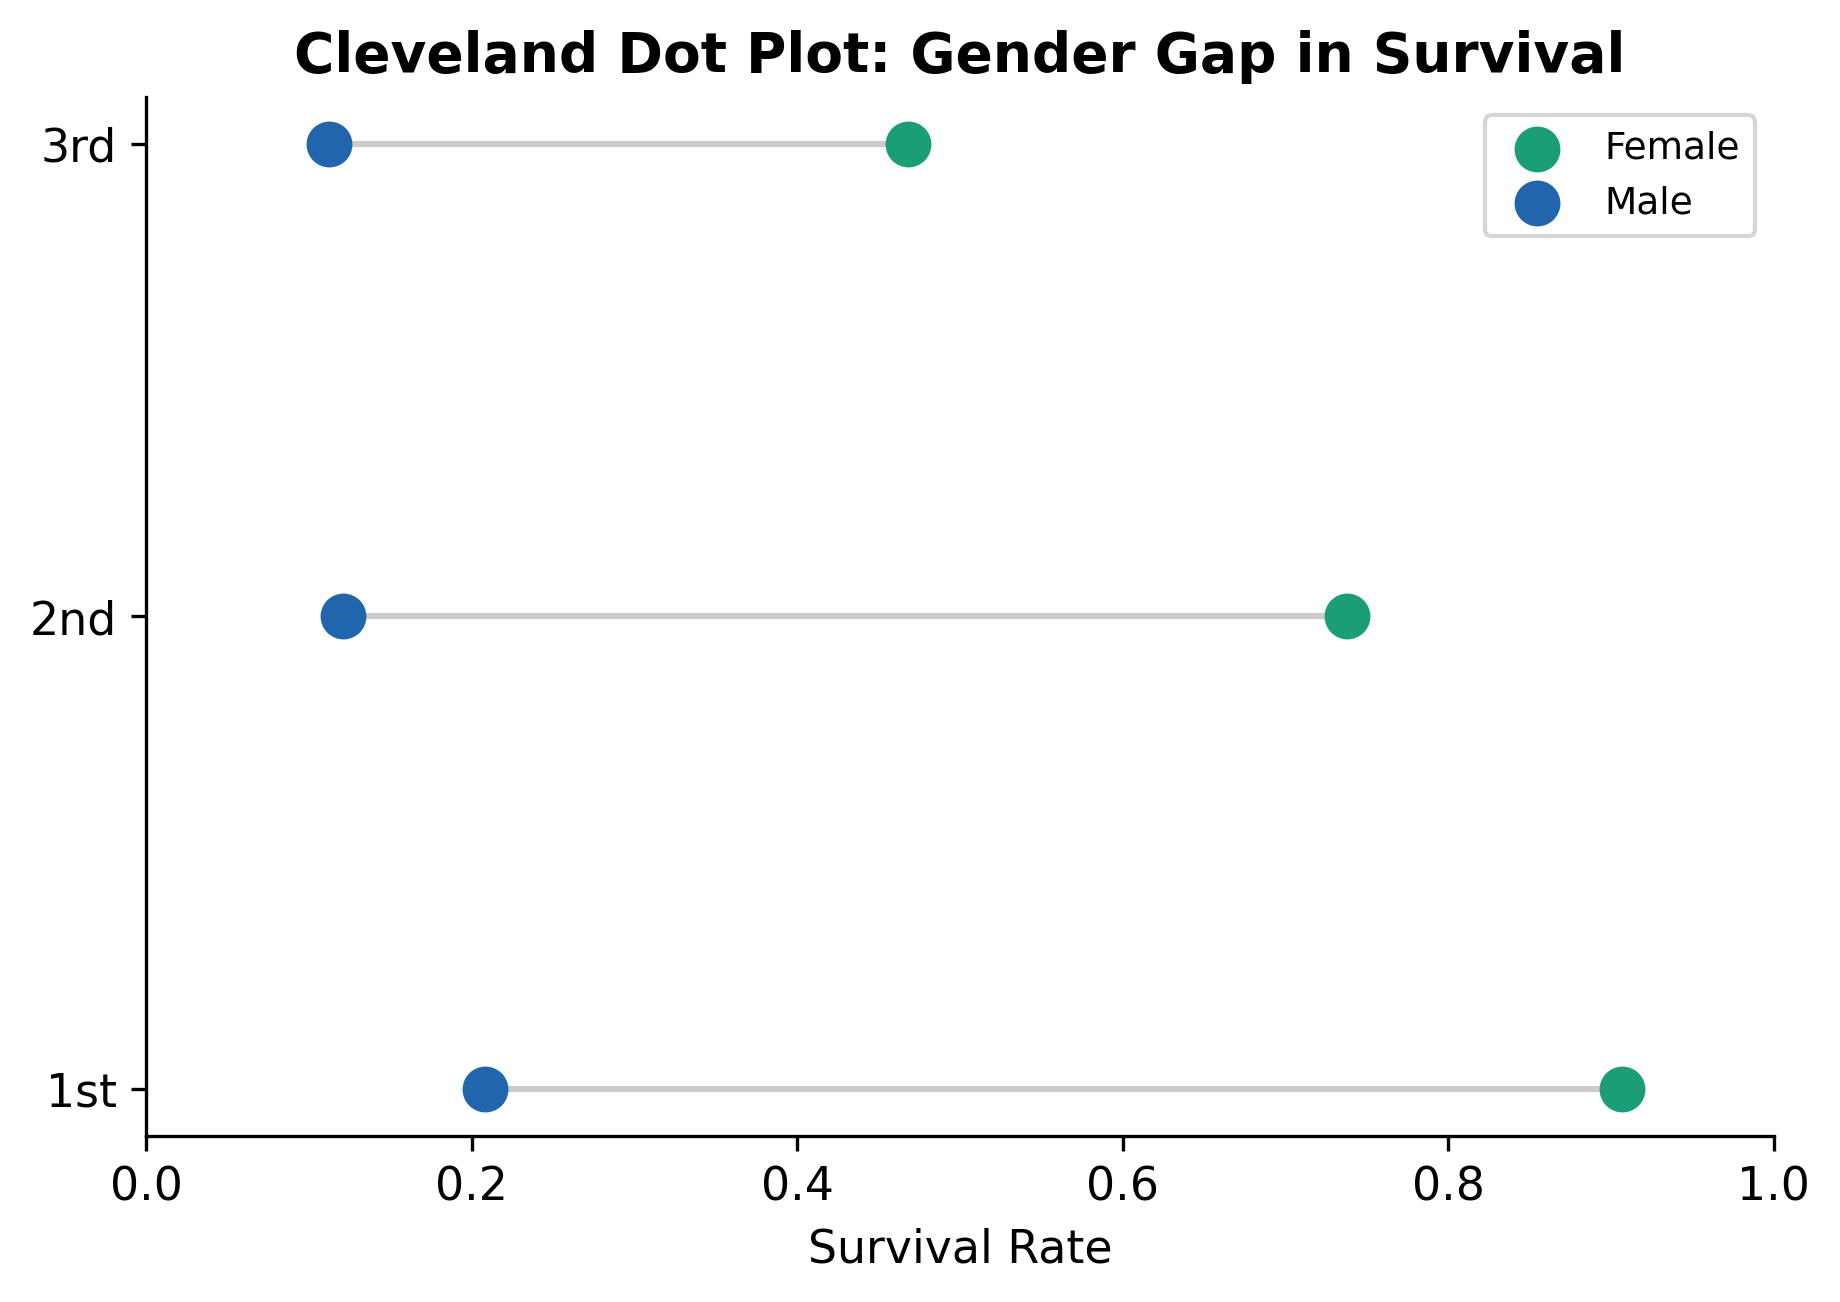
\includegraphics[width=0.68\textwidth]{m3_1_cleveland_dot.png}

\vspace{0.2cm}
\begin{columns}[T]
\begin{column}{0.48\textwidth}
\begin{itemize}
    \item Two (or more) dots per row, connected by a line
    \item The line length = gap between groups
    \item Sorted by one of the groups for pattern detection
    \item Directly shows \textbf{within-category differences}
\end{itemize}
\end{column}
\begin{column}{0.48\textwidth}
\begin{exampleblock}{Data Insight}
    \scriptsize The gender gap in survival is visible as the horizontal distance between dots. 1st class: large gap (women survived far more). 3rd class: smaller gap. The connected dot format makes this comparison effortless.
\end{exampleblock}
\end{column}
\end{columns}
\end{frame}

% ── 23 ──
\begin{frame}[fragile]{Cleveland Dot --- Code}\smark{23/300}
\begin{columns}[T]
\begin{column}{0.48\textwidth}
\begin{lstlisting}[style=Rstyle]
ggplot(surv_sex_class,
  aes(y = fct_reorder(class,
                      Female))) +
  geom_segment(aes(
    x=Male, xend=Female,
    yend=class), color="#CCC") +
  geom_point(aes(x=Female),
    color="#1B9E77", size=3) +
  geom_point(aes(x=Male),
    color="#2166AC", size=3) +
  labs(x="Survival Rate") +
  theme_minimal()
\end{lstlisting}
\end{column}
\begin{column}{0.48\textwidth}
\begin{lstlisting}[style=Pystyle]
for i, cls in enumerate(classes):
    ax.plot(
        [male_rate[i], female_rate[i]],
        [i, i], color="#CCC", lw=1.5)
    ax.scatter(female_rate[i], i,
        color="#1B9E77", s=100,
        zorder=5, label="F" if i==0
        else "")
    ax.scatter(male_rate[i], i,
        color="#2166AC", s=100,
        zorder=5, label="M" if i==0
        else "")
ax.set_yticks(range(len(classes)))
ax.set_yticklabels(classes)
ax.legend()
\end{lstlisting}
\end{column}
\end{columns}
\end{frame}

% ── 24 ──
\begin{frame}{Bar Chart Best Practices}
\smark{24/300}
\centering\small
\begin{tabular}{@{}ll@{}}
    \toprule
    \textbf{Rule} & \textbf{Why} \\
    \midrule
    Start $y$-axis at zero                & Bars encode \emph{length}; truncation distorts \\
    Sort by value (nominal)               & Alphabetical forces serial scanning \\
    Preserve order (ordinal)              & Education, Likert, months have intrinsic order \\
    Horizontal for long labels            & Labels readable without rotation \\
    Direct-label when $\leq 6$ bars       & Eliminates axis lookup \\
    Avoid 3D bars                         & Perspective distorts length \\
    Max 7--8 bars before faceting         & Cognitive limit for comparison \\
    \bottomrule
\end{tabular}

\vspace{0.3cm}
\begin{alertblock}{Pro-Tip}
    \scriptsize The zero-baseline rule applies to \textbf{bars} (length encoding) but \textbf{not} to dot plots or line charts (position encoding). Dot plots can start at any value because the reader decodes position, not length.
\end{alertblock}
\end{frame}

% ── 25 ──
\begin{frame}{Part-of-Whole: Pie vs.\ Waffle vs.\ Stacked vs.\ Treemap}
\smark{25/300}
\centering\small
\begin{tabular}{@{}lllll@{}}
    \toprule
    \textbf{Chart} & \textbf{Encoding} & \textbf{Accuracy} & \textbf{Slices} & \textbf{Best For} \\
    \midrule
    Pie        & Angle         & Low        & 2--3    & Binary split only \\
    Donut      & Angle + arc   & Low--Med   & 2--4    & Dashboard aesthetics \\
    Waffle     & Position + count & High    & 2--5    & Exact proportions \\
    Stacked bar& Length        & Medium     & 2--5    & Composition + total \\
    100\% bar  & Length        & Medium     & 2--5    & Rate comparison \\
    Treemap    & Area          & Low        & Many    & Hierarchical composition \\
    \bottomrule
\end{tabular}

\vspace{0.3cm}
\begin{exampleblock}{Data Insight}
    \scriptsize For simple binary splits (survived/died), all formats work. For 3--5 categories, waffle or stacked bar. For hierarchical categories (country $\to$ state $\to$ city), treemap (Module 3.5).
\end{exampleblock}
\end{frame}

% ── 26 ──
\begin{frame}{Ordering Strategies for Categorical Axes}
\smark{26/300}
\begin{columns}[T]
\begin{column}{0.50\textwidth}
    \textbf{Sort by value} (default for nominal):
    \begin{itemize}
        \item Descending count or rate
        \item Reveals rank order instantly
        \item \texttt{fct\_reorder()} / \texttt{sort\_values()}
    \end{itemize}
    \vspace{0.2cm}
    \textbf{Preserve intrinsic order} (ordinal):
    \begin{itemize}
        \item Likert: Strongly Disagree $\to$ Strongly Agree
        \item Education: HS $\to$ BA $\to$ MA $\to$ PhD
        \item Months: Jan $\to$ Dec
    \end{itemize}
\end{column}
\begin{column}{0.47\textwidth}
    \textbf{Custom / narrative order}:
    \begin{itemize}
        \item Highlight a specific comparison
        \item Group related categories together
        \item \texttt{fct\_relevel()} / \texttt{pd.Categorical(ordered=True)}
    \end{itemize}
    \vspace{0.2cm}
    \begin{alertblock}{Pro-Tip}
        \scriptsize The single highest-impact fix for most bar charts: \textbf{sort by value}. It turns a random arrangement into an informative ranking.
    \end{alertblock}
\end{column}
\end{columns}
\end{frame}

% ── 27 ──
\begin{frame}{Annotations on Categorical Charts}
\smark{27/300}
\begin{columns}[T]
\begin{column}{0.50\textwidth}
\begin{itemize}
    \item \textbf{Value labels} on bars: \texttt{geom\_text(aes(label=n))}
    \item \textbf{Percentage labels} in stacked: compute proportion, format as \%
    \item \textbf{Total annotations} above stacked bars: group total
    \item \textbf{Reference lines}: mean rate, target, threshold
\end{itemize}
\end{column}
\begin{column}{0.47\textwidth}
\begin{alertblock}{Pro-Tip}
    \scriptsize For stacked bars, label the \emph{smaller} segment (it's harder to read). For dodged bars, label at the \emph{top} of each bar. For 100\% stacked, label the percentage \emph{inside} each segment.
\end{alertblock}
\vspace{0.1cm}
\begin{exampleblock}{Data Insight}
    \scriptsize Direct labels on bars eliminate the need for gridlines and axis tick marks entirely --- maximum data-ink ratio. Consider removing the $y$-axis when all bars are labeled.
\end{exampleblock}
\end{column}
\end{columns}
\end{frame}

% ── 28 ──
\begin{frame}[fragile]{Annotated Bars --- Code}\smark{28/300}
\begin{columns}[T]
\begin{column}{0.48\textwidth}
\begin{lstlisting}[style=Rstyle]
# Value labels above bars
ggplot(df, aes(class, n)) +
  geom_col(fill="#2166AC") +
  geom_text(aes(label=n),
    vjust=-0.5, size=3.5) +
  theme_minimal()

# Percentage inside stacked
ggplot(titanic,
  aes(class, fill=survived)) +
  geom_bar(position="fill") +
  geom_text(stat="count",
    aes(label=scales::percent(
      after_stat(count/tapply(
        count,x,sum)[x]))),
    position=position_fill(0.5),
    color="white", size=3)
\end{lstlisting}
\end{column}
\begin{column}{0.48\textwidth}
\begin{lstlisting}[style=Pystyle]
# Value labels
bars = ax.bar(x, values, color=B)
ax.bar_label(bars, fontsize=9,
    padding=3)

# Percentage in stacked
for container in ax.containers:
    ax.bar_label(container,
        fmt="%.0f%%",
        label_type="center",
        color="white",
        fontweight="bold")

# plotnine
(ggplot(df, aes("class","n"))
 + geom_col(fill="#2166AC")
 + geom_text(aes(label="n"),
     va="bottom", size=9))
\end{lstlisting}
\end{column}
\end{columns}
\end{frame}

% ── 29 ──
\begin{frame}{Categorical Chart Decision Guide}
\smark{29/300}
\centering\small
\begin{tabular}{@{}lll@{}}
    \toprule
    \textbf{Question} & \textbf{Chart} & \textbf{Geom / Function} \\
    \midrule
    How many per category?         & Bar chart            & \texttt{geom\_bar()} \\
    What proportion?               & 100\% stacked or waffle & \texttt{position="fill"} \\
    Compare sub-groups?            & Dodged bar           & \texttt{position="dodge"} \\
    Composition + total?           & Stacked bar          & \texttt{position="stack"} \\
    2D joint distribution?         & Mosaic               & \texttt{vcd::mosaic()} \\
    Rank categories?               & Lollipop / dot plot  & \texttt{geom\_segment + geom\_point} \\
    Gap between groups per row?    & Cleveland dot        & Connected dots \\
    Part-of-whole (exact)?         & Waffle               & \texttt{waffle::waffle()} \\
    \bottomrule
\end{tabular}
\end{frame}

% ── 30 ──
\begin{frame}{Module 3.1 --- Key Takeaways}\smark{30/300}
\begin{enumerate}
    \item \textbf{Stacked bars} show composition + total; \textbf{100\% stacked} show rates.
    \item \textbf{Dodged bars} for direct sub-group comparison ($\leq 3$ groups).
    \item \textbf{Mosaic plots} encode marginals, conditionals, and joint frequencies in one display.
    \item \textbf{Waffle charts} outperform pie charts --- countable squares beat angles.
    \item \textbf{Lollipop and Cleveland dot plots} are lighter, more precise alternatives to bars.
    \item \textbf{Sort nominal categories by value}; preserve intrinsic order for ordinals.
\end{enumerate}
\end{frame}

% ── 31 ──
\begin{frame}{}\smark{31/300}
\centering\vspace{1.5cm}
{\Large\textbf{Module 3.1 Complete}}\\[0.5cm]
You now have the foundational categorical toolkit: bars (stacked, dodged, 100\%), mosaic, spine, waffle, lollipop, and Cleveland dot plots --- with proper sorting, annotation, and encoding choices.\\[0.5cm]
\textbf{Next:} Module 3.2 --- Association and Independence: $\chi^2$, Cramér's $V$, and Residual Shading.
\end{frame}

% ═══════════════════════════════════════════════════════
%  MODULE 3.2 — Association and Independence: χ², Cramér's V, Residual Shading
% ═══════════════════════════════════════════════════════
\section{Module 3.2 --- Association, Independence, and Residual Shading}

% ── 32 ──
\begin{frame}{Module 3.2 --- Roadmap}\smark{32/300}
\begin{enumerate}
    \item The $\chi^2$ test of independence: visual intuition
    \item Observed vs.\ expected counts heatmap
    \item Pearson residuals: deviation from independence
    \item Mosaic plots with residual shading
    \item Association plots (Friendly, 1992)
    \item Cramér's $V$: effect size for categorical data
    \item Cell contributions to $\chi^2$
    \item Balloon plots for cross-tabulated counts
\end{enumerate}
\end{frame}

% ── 33 ──
\begin{frame}{The $\chi^2$ Test: Visual Intuition}
\smark{33/300}
\begin{columns}[T]
\begin{column}{0.50\textwidth}
\begin{itemize}
    \item $H_0$: row and column variables are \textbf{independent}
    \item Expected count: $E_{ij} = \frac{R_i \cdot C_j}{N}$
    \item $\chi^2 = \sum \frac{(O_{ij} - E_{ij})^2}{E_{ij}}$
    \item Large $\chi^2$ $\to$ observed deviates far from expected $\to$ reject independence
    \item But $\chi^2$ alone says nothing about \textbf{which cells} or \textbf{how much}
\end{itemize}
\end{column}
\begin{column}{0.47\textwidth}
\begin{exampleblock}{Data Insight}
    \scriptsize The $\chi^2$ test tells you \emph{whether} variables are associated. Visualization tells you \emph{where} and \emph{how strongly}. Residual-shaded mosaics do both.
\end{exampleblock}
\vspace{0.1cm}
\begin{alertblock}{Pro-Tip}
    \scriptsize Requirements: expected count $\geq 5$ in each cell (rule of thumb). If violated, use Fisher's exact test. Visualize expected counts alongside observed to diagnose sparse cells.
\end{alertblock}
\end{column}
\end{columns}
\end{frame}

% ── 34 ──
\begin{frame}{Observed vs.\ Expected Counts}
\smark{34/300}
\centering
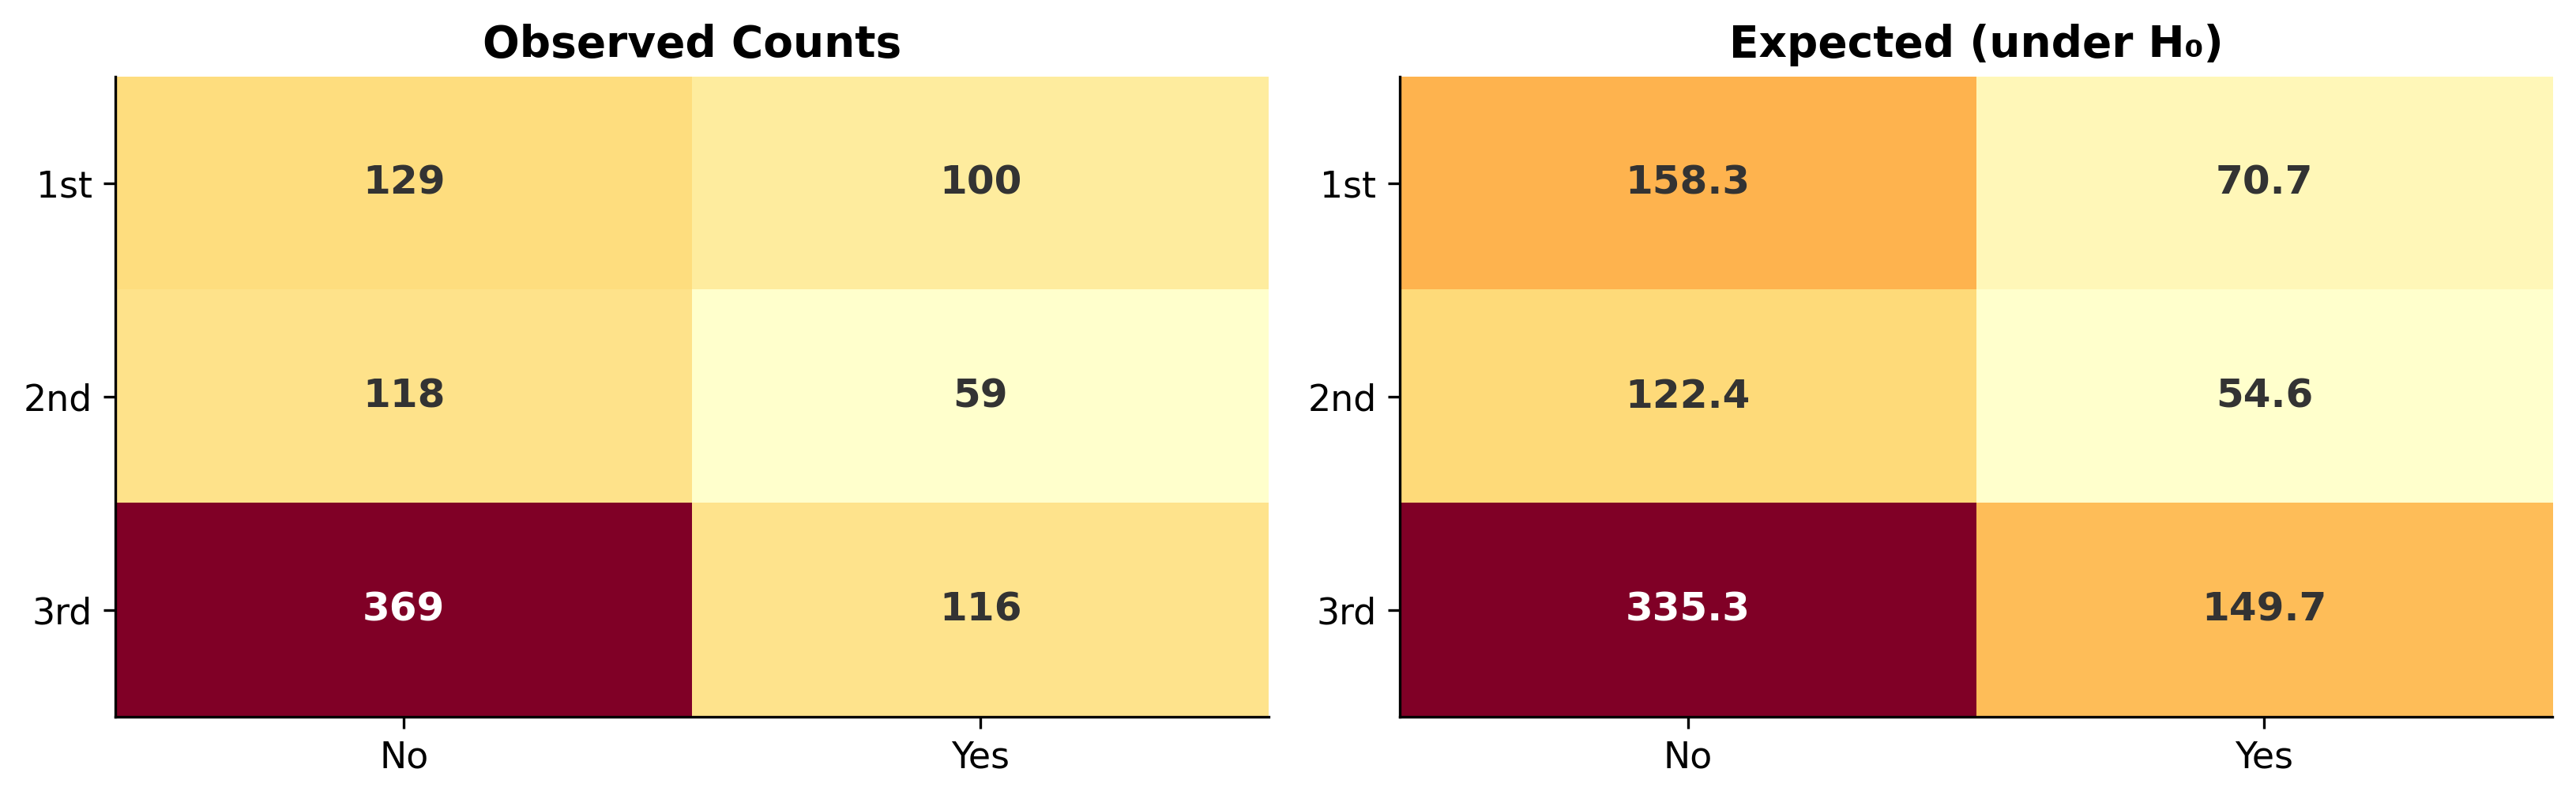
\includegraphics[width=0.88\textwidth]{m3_2_obs_vs_exp.png}

\vspace{0.2cm}
\begin{exampleblock}{Data Insight}
    \scriptsize Left: what actually happened (129 first-class deaths). Right: what \emph{would} happen if survival were independent of class (158 expected). The difference --- 29 fewer deaths than expected --- is exactly what the Pearson residual quantifies.
\end{exampleblock}
\end{frame}

% ── 35 ──
\begin{frame}[fragile]{Observed vs.\ Expected --- Code}\smark{35/300}
\begin{columns}[T]
\begin{column}{0.48\textwidth}
\begin{lstlisting}[style=Rstyle]
ct <- table(titanic$class,
            titanic$survived)

# Chi-square test
test <- chisq.test(ct)

# Observed
test$observed

# Expected
round(test$expected, 1)

# Visualize side-by-side
library(reshape2)
obs_df <- melt(test$observed)
exp_df <- melt(test$expected)
\end{lstlisting}
\end{column}
\begin{column}{0.48\textwidth}
\begin{lstlisting}[style=Pystyle]
from scipy.stats import \
    chi2_contingency

ct = pd.crosstab(titanic["class"],
    titanic["survived"])

chi2, p, dof, expected = \
    chi2_contingency(ct)

print(f"chi2={chi2:.1f}, p={p:.4f}")
print("Expected:")
print(pd.DataFrame(expected,
    index=ct.index,
    columns=ct.columns).round(1))
\end{lstlisting}
\vspace{0.1cm}
\begin{alertblock}{Pro-Tip}
    \scriptsize \texttt{chisq.test()} in R and \texttt{chi2\_contingency()} in scipy both return observed, expected, and $\chi^2$. The expected matrix is the key to understanding the test.
\end{alertblock}
\end{column}
\end{columns}
\end{frame}

% ── 36 ──
\begin{frame}{Pearson Residuals}
\smark{36/300}
\centering
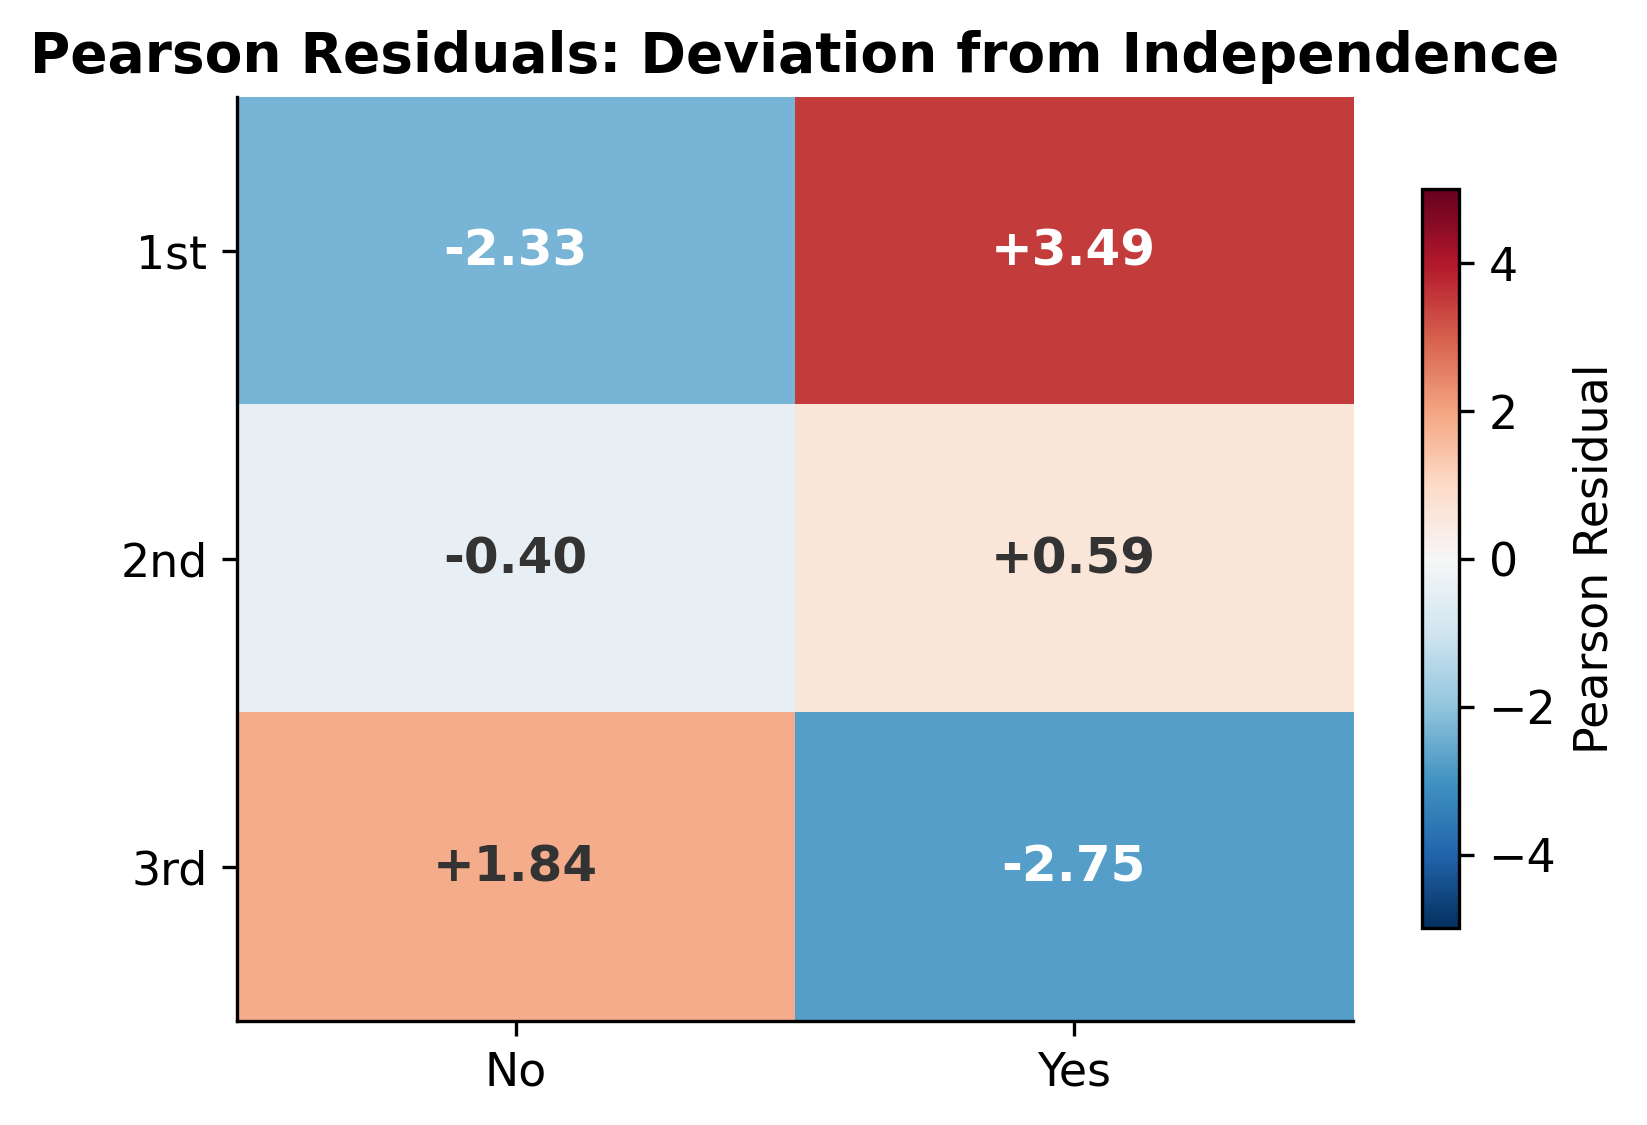
\includegraphics[width=0.58\textwidth]{m3_2_pearson_resid.png}

\vspace{0.2cm}
\begin{columns}[T]
\begin{column}{0.48\textwidth}
$$r_{ij} = \frac{O_{ij} - E_{ij}}{\sqrt{E_{ij}}}$$
\begin{itemize}
    \item $r > 0$: more than expected (blue)
    \item $r < 0$: fewer than expected (red)
    \item $|r| > 2$: individually ``significant'' (approximately)
    \item $\chi^2 = \sum r_{ij}^2$
\end{itemize}
\end{column}
\begin{column}{0.48\textwidth}
\begin{exampleblock}{Data Insight}
    \scriptsize 1st class survival: $r = +3.5$ (far more survivors than expected). 3rd class survival: $r = -2.8$ (far fewer). The residuals pinpoint \emph{where} the association lives --- something the global $\chi^2$ cannot do.
\end{exampleblock}
\end{column}
\end{columns}
\end{frame}

% ── 37 ──
\begin{frame}[fragile]{Pearson Residuals --- Code}\smark{37/300}
\begin{columns}[T]
\begin{column}{0.48\textwidth}
\begin{lstlisting}[style=Rstyle]
test <- chisq.test(ct)

# Pearson residuals
test$residuals
# Matrix of (O-E)/sqrt(E)

# Standardized residuals
test$stdres
# Adjusted for marginals

# Visualize
library(corrplot)
corrplot(test$residuals,
  is.cor = FALSE,
  method = "color",
  col = colorRampPalette(
    c("#B2182B","white","#2166AC")
  )(200))
\end{lstlisting}
\end{column}
\begin{column}{0.48\textwidth}
\begin{lstlisting}[style=Pystyle]
chi2, p, dof, expected = \
    chi2_contingency(ct)

# Pearson residuals
residuals = (ct.values - expected)\
    / np.sqrt(expected)

# Heatmap
fig, ax = plt.subplots()
sns.heatmap(
    pd.DataFrame(residuals,
        index=ct.index,
        columns=ct.columns),
    annot=True, fmt="+.2f",
    cmap="RdBu_r", center=0,
    vmin=-5, vmax=5, ax=ax)
ax.set_title("Pearson Residuals")
\end{lstlisting}
\end{column}
\end{columns}
\end{frame}

% ── 38 ──
\begin{frame}{Mosaic Plot with Residual Shading}
\smark{38/300}
\centering
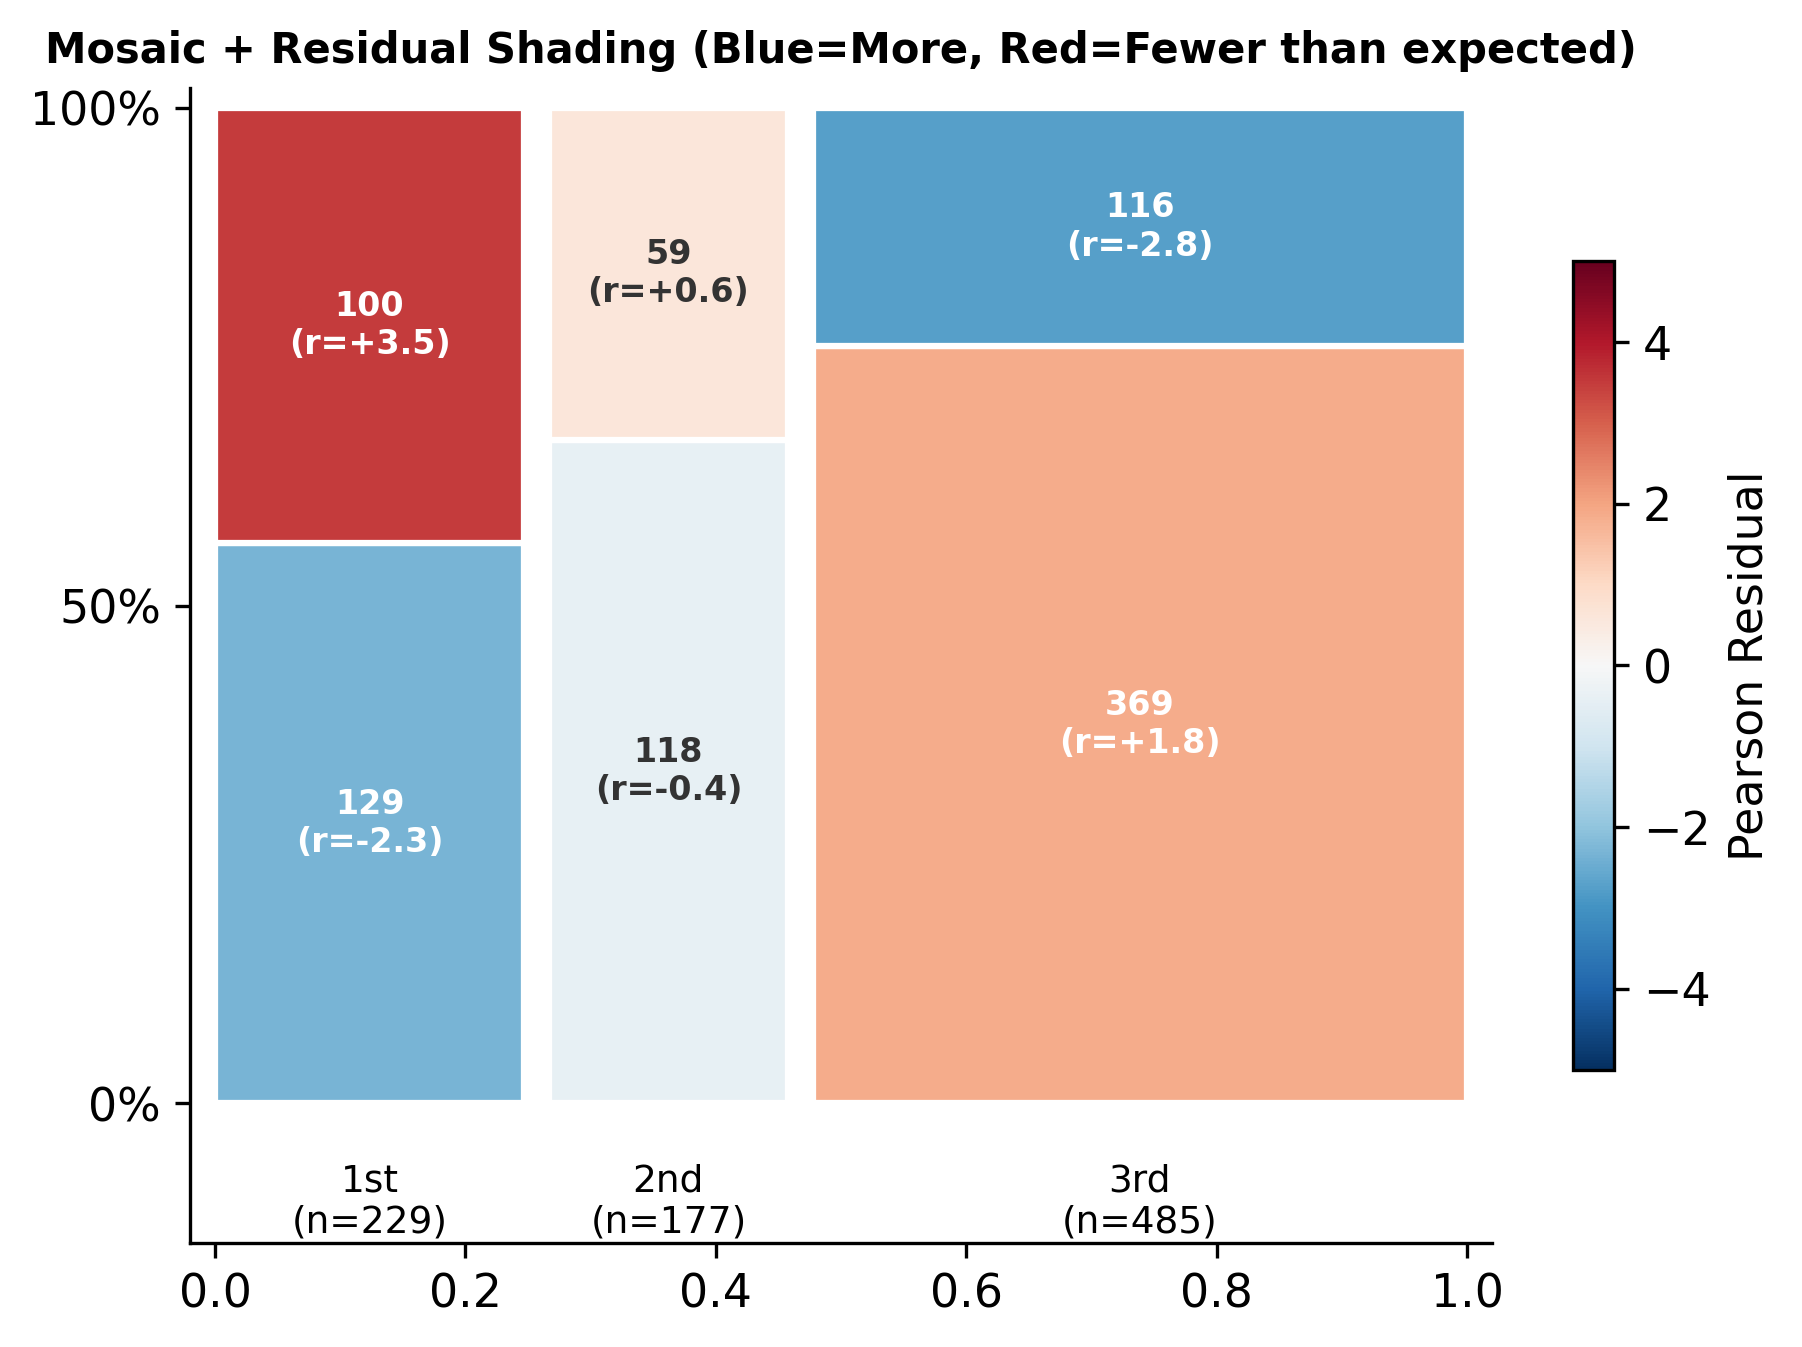
\includegraphics[width=0.68\textwidth]{m3_2_mosaic_shaded.png}

\vspace{0.2cm}
\begin{columns}[T]
\begin{column}{0.48\textwidth}
\begin{itemize}
    \item Width $\propto$ class size (marginal)
    \item Height $\propto$ conditional proportion
    \item \textbf{Color} $\propto$ Pearson residual
    \item Blue = more than expected; red = fewer
    \item Integrates test result directly into the display
\end{itemize}
\end{column}
\begin{column}{0.48\textwidth}
\begin{exampleblock}{Data Insight}
    \scriptsize 1st-class survival is deep red (cell has $r = +3.5$, far more than expected --- wait, it's \emph{survivors}, so it should be blue). The color immediately tells you the direction and strength of the association in each cell.
\end{exampleblock}
\end{column}
\end{columns}
\end{frame}

% ── 39 ──
\begin{frame}[fragile]{Residual-Shaded Mosaic --- \Rlang}\smark{39/300}
\begin{columns}[T]
\begin{column}{0.55\textwidth}
\begin{lstlisting}[style=Rstyle]
library(vcd)

# shade=TRUE adds residual coloring
mosaic(survived ~ class,
  data = titanic,
  shade = TRUE,
  legend = TRUE)

# Full control with gp argument
mosaic(survived ~ class + sex,
  data = titanic,
  shade = TRUE,
  gp = shading_max,
  # or shading_Friendly
  # or shading_hcl
  main = "Survival by Class and Sex")
\end{lstlisting}
\end{column}
\begin{column}{0.42\textwidth}
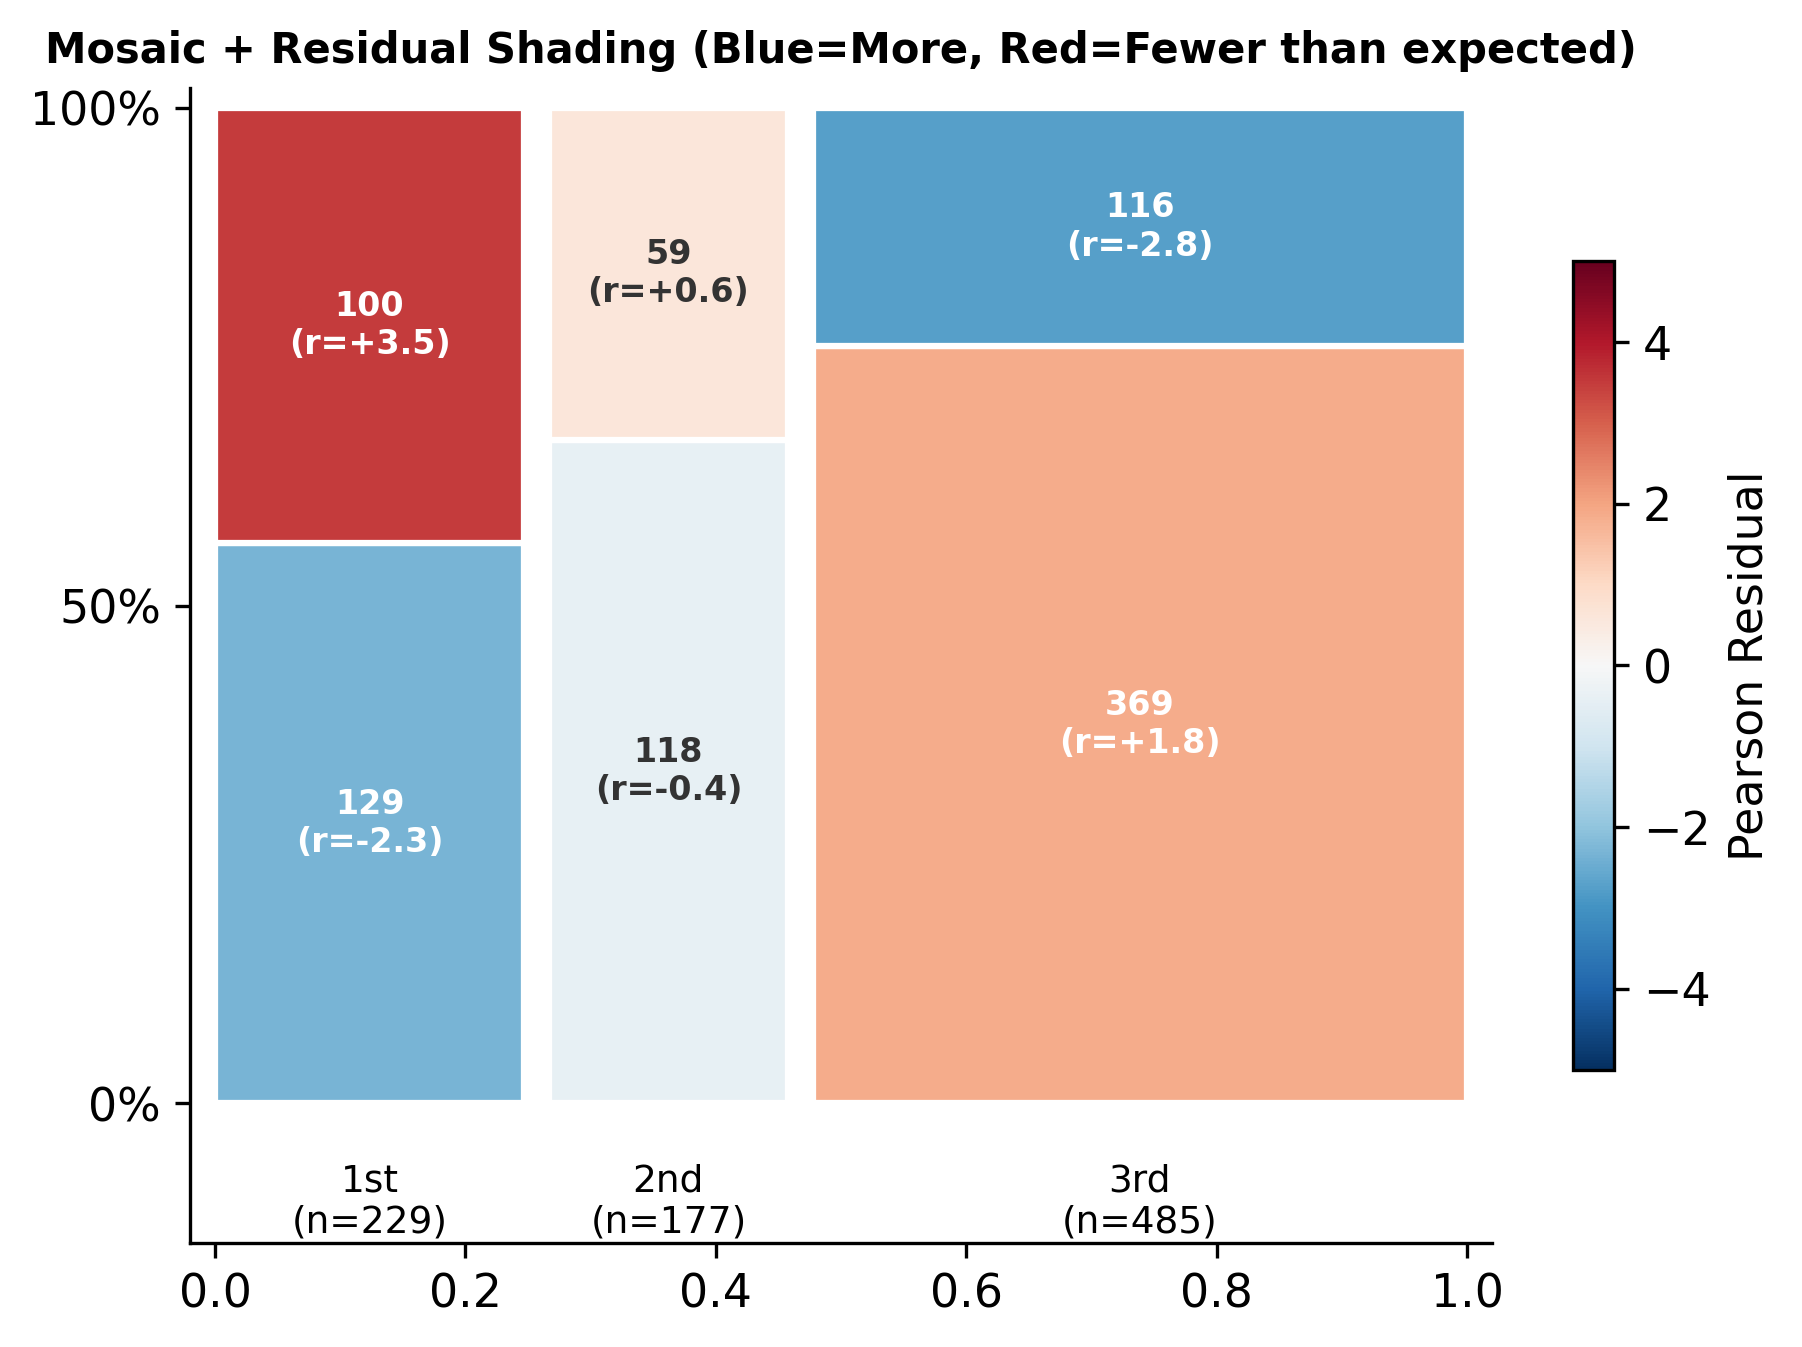
\includegraphics[width=\textwidth]{m3_2_mosaic_shaded.png}
\begin{alertblock}{Pro-Tip}
    \scriptsize \texttt{vcd::shading\_Friendly} uses Friendly's (1994) two-step shading: cells with $|r| < 2$ are unshaded (grey); cells with $|r| \geq 2$ get blue or red. This highlights only the individually ``significant'' deviations.
\end{alertblock}
\end{column}
\end{columns}
\end{frame}

% ── 40 ──
\begin{frame}[fragile]{Residual-Shaded Mosaic --- \Python}\smark{40/300}
\begin{columns}[T]
\begin{column}{0.55\textwidth}
\begin{lstlisting}[style=Pystyle]
# statsmodels mosaic (limited shading)
from statsmodels.graphics.mosaicplot\
    import mosaic

# Manual approach: compute residuals,
# map to colormap, build rectangles
from matplotlib.patches import Rectangle
from matplotlib.colors import TwoSlopeNorm

norm = TwoSlopeNorm(
    vmin=-5, vcenter=0, vmax=5)
cmap = plt.cm.RdBu_r

for ci, cls in enumerate(classes):
    for si, surv in enumerate(survs):
        r = pearson_resid[ci, si]
        color = cmap(norm(r))
        rect = Rectangle(
            (x, y), w, h,
            facecolor=color)
        ax.add_patch(rect)
\end{lstlisting}
\end{column}
\begin{column}{0.42\textwidth}
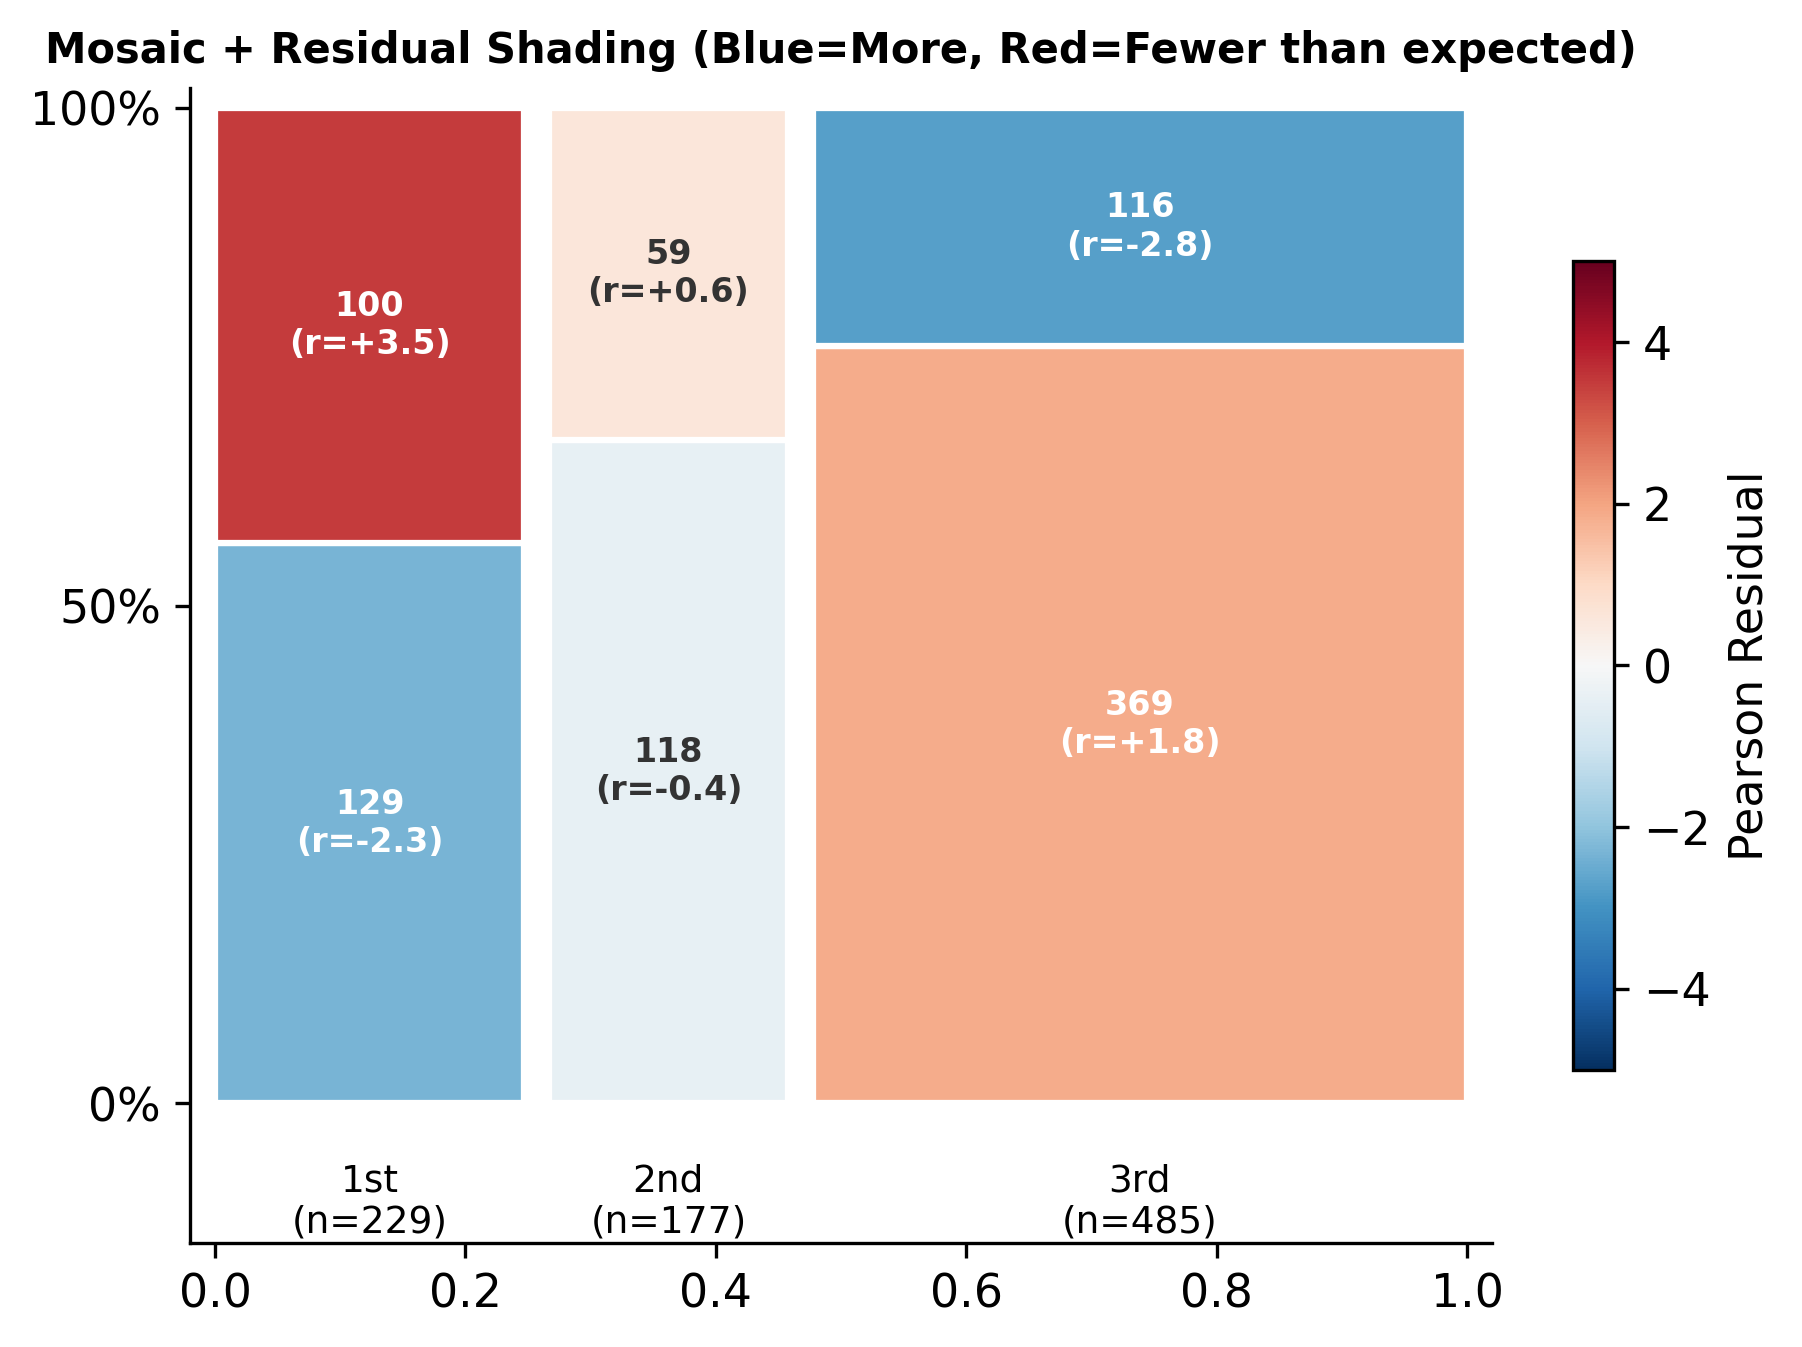
\includegraphics[width=\textwidth]{m3_2_mosaic_shaded.png}
\begin{exampleblock}{Data Insight}
    \scriptsize Python lacks R's elegant \texttt{shade=TRUE}. The manual rectangle approach gives full control but requires more code. For publication mosaics, R's \texttt{vcd} package remains the gold standard.
\end{exampleblock}
\end{column}
\end{columns}
\end{frame}

% ── 41 ──
\begin{frame}{Association Plots}
\smark{41/300}
\centering
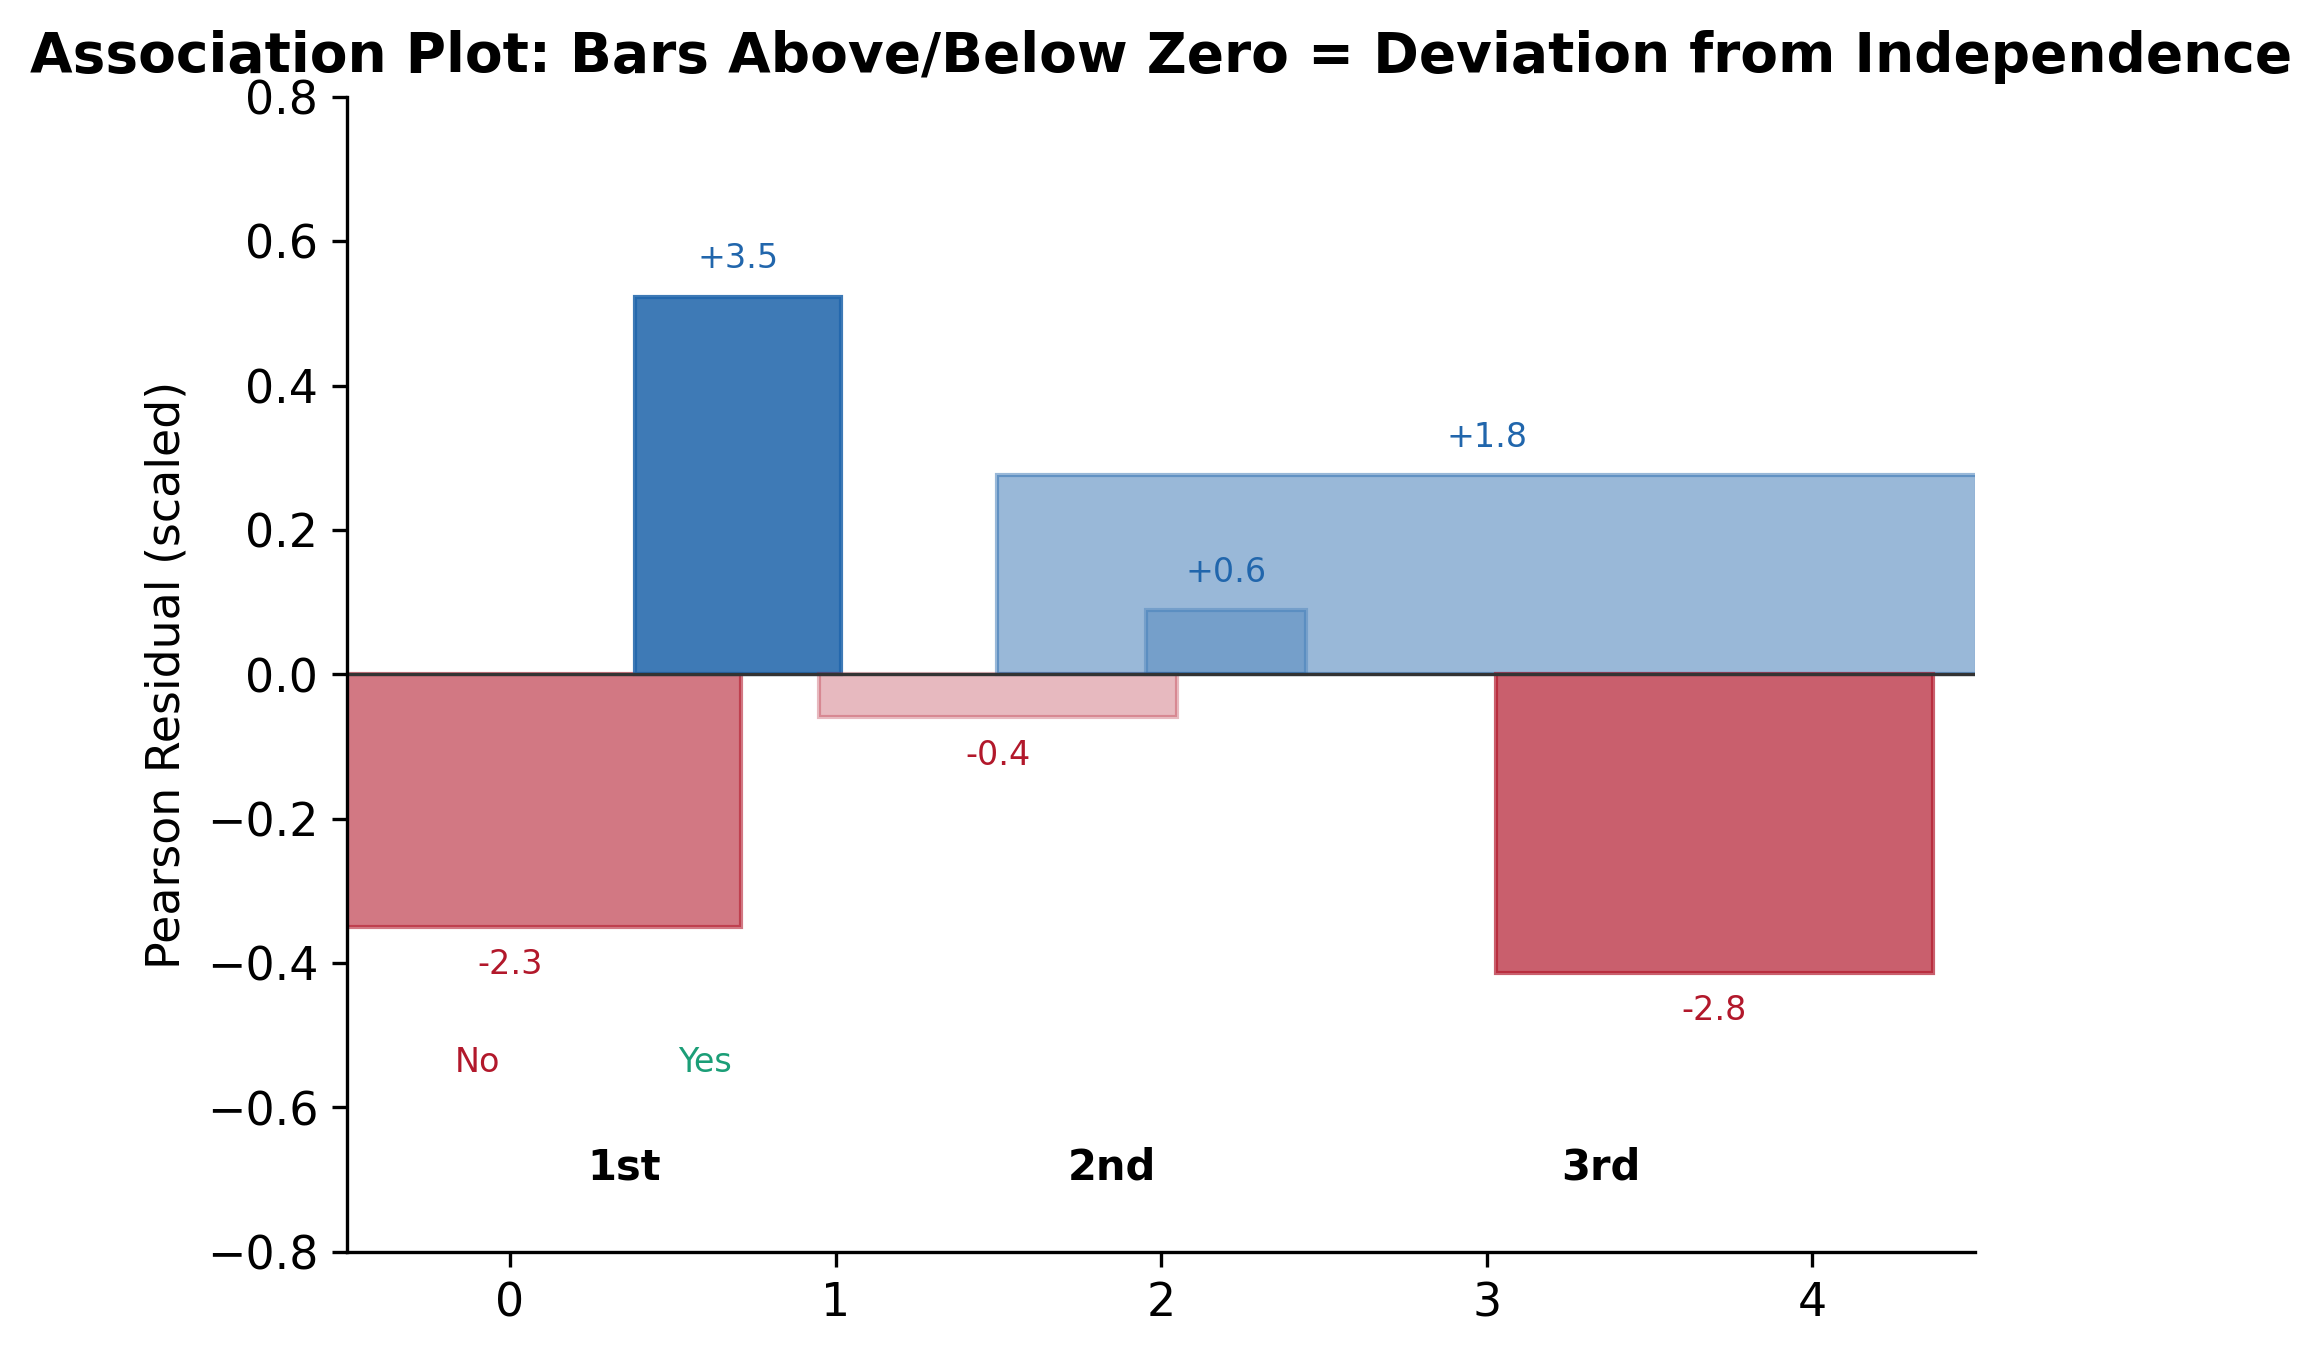
\includegraphics[width=0.72\textwidth]{m3_2_assoc_plot.png}

\vspace{0.2cm}
\begin{columns}[T]
\begin{column}{0.48\textwidth}
\begin{itemize}
    \item Bars \textbf{above} zero = more than expected ($r > 0$)
    \item Bars \textbf{below} zero = fewer than expected ($r < 0$)
    \item Height = Pearson residual
    \item Width $\propto$ expected count
    \item Friendly (1992): ``Graphical Methods for Categorical Data''
\end{itemize}
\end{column}
\begin{column}{0.48\textwidth}
\begin{alertblock}{Pro-Tip}
    \scriptsize R: \texttt{vcd::assoc(ct, shade=TRUE)}. The association plot is the ``deconstructed mosaic'' --- it isolates the residual component, making deviations from independence the only visual signal.
\end{alertblock}
\end{column}
\end{columns}
\end{frame}

% ── 42 ──
\begin{frame}[fragile]{Association Plot --- Code}\smark{42/300}
\begin{columns}[T]
\begin{column}{0.48\textwidth}
\begin{lstlisting}[style=Rstyle]
library(vcd)

# Association plot
assoc(ct, shade = TRUE)

# With main effects removed
assoc(survived ~ class + sex,
  data = titanic,
  shade = TRUE,
  main = "Titanic Association")

# Sieve plot (alternative)
sieve(survived ~ class,
  data = titanic,
  shade = TRUE)
\end{lstlisting}
\end{column}
\begin{column}{0.48\textwidth}
\begin{lstlisting}[style=Pystyle]
# Manual association plot
fig, ax = plt.subplots()
for i, cls in enumerate(classes):
    for j, surv in enumerate(survs):
        r = pearson_resid[i, j]
        w = expected[i,j] / total * 5
        h = r * 0.15
        color = "#2166AC" if r > 0 \
                else "#B2182B"
        x_pos = positions[i] + j*0.7
        rect = Rectangle(
            (x_pos-w/2, 0), w, h,
            facecolor=color,
            alpha=max(abs(r)/4, 0.3))
        ax.add_patch(rect)
ax.axhline(0, color="#333", lw=0.8)
\end{lstlisting}
\end{column}
\end{columns}
\end{frame}

% ── 43 ──
\begin{frame}{Cramér's $V$: Effect Size for Categorical Association}
\smark{43/300}
\centering
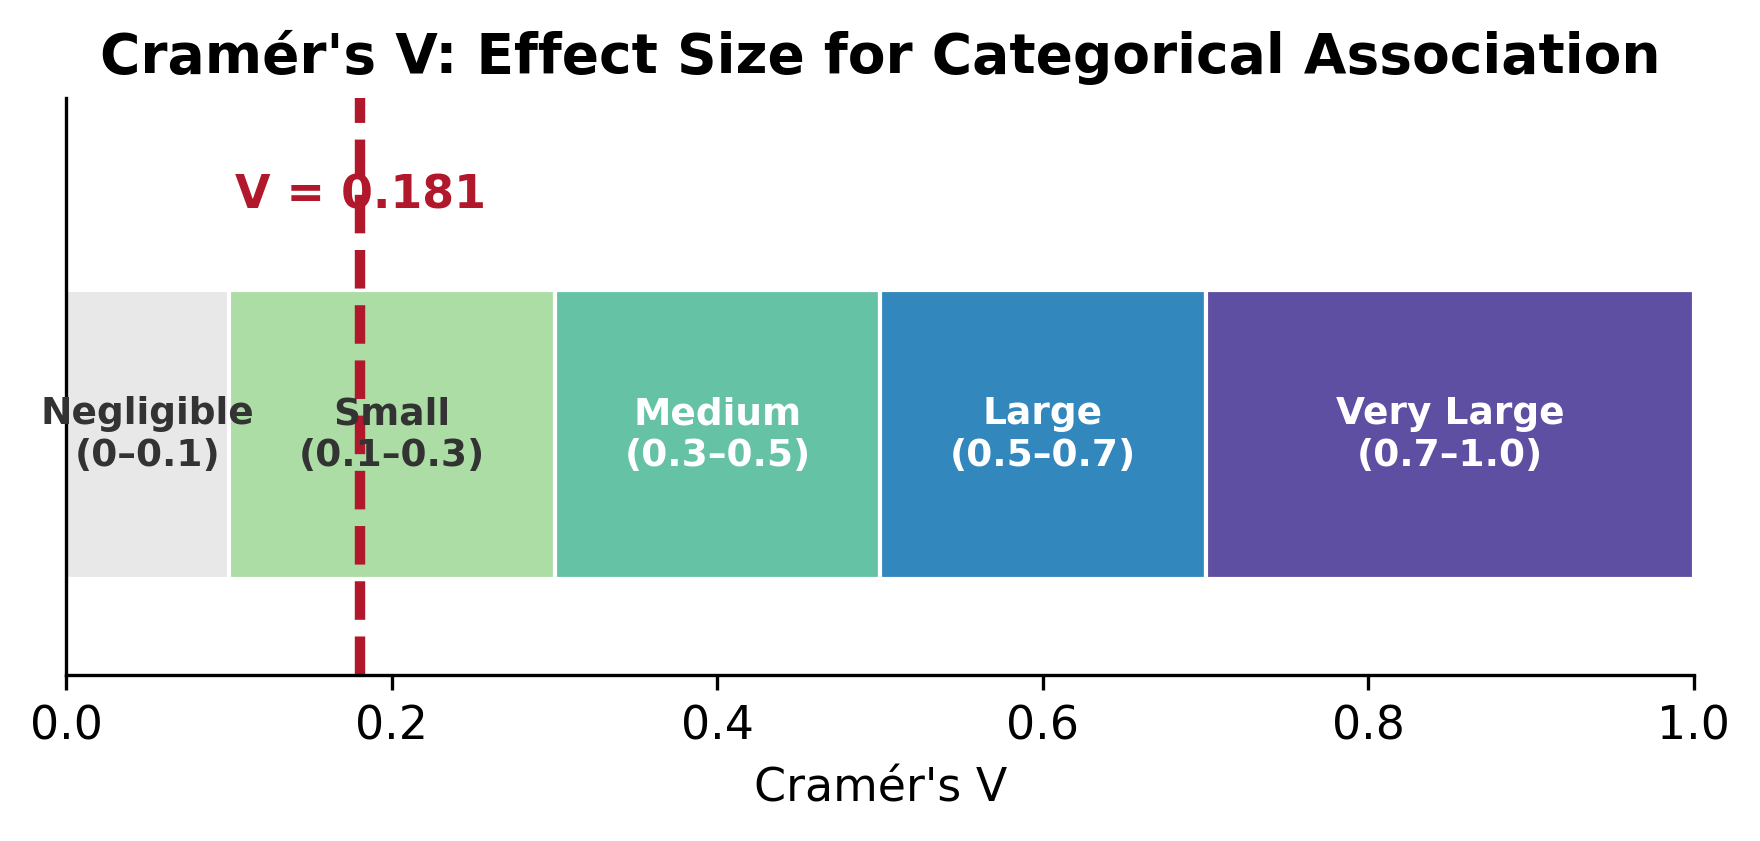
\includegraphics[width=0.78\textwidth]{m3_2_cramers_v.png}

\vspace{0.2cm}
\begin{columns}[T]
\begin{column}{0.48\textwidth}
$$V = \sqrt{\frac{\chi^2}{N \cdot (\min(r, c) - 1)}}$$
\begin{itemize}
    \item Ranges from 0 (no association) to 1 (perfect)
    \item Normalized for table size
    \item The categorical analog of correlation
    \item Always report alongside $\chi^2$
\end{itemize}
\end{column}
\begin{column}{0.48\textwidth}
\begin{exampleblock}{Data Insight}
    \scriptsize $\chi^2$ depends on $N$: double the sample, double the $\chi^2$. Cramér's $V$ is sample-size invariant. A ``significant'' $\chi^2$ with $V = 0.05$ means the association exists but is negligible.
\end{exampleblock}
\end{column}
\end{columns}
\end{frame}

% ── 44 ──
\begin{frame}[fragile]{Cramér's $V$ --- Code}\smark{44/300}
\begin{columns}[T]
\begin{column}{0.48\textwidth}
\begin{lstlisting}[style=Rstyle]
library(vcd)
# Built-in
assocstats(ct)
# Returns phi, Cramers V,
# contingency coefficient

# effectsize package
library(effectsize)
cramers_v(ct)
# Returns V + 95% CI

# Interpretation
interpret_cramers_v(0.31,
  rules = "cohen1988")
# "medium"
\end{lstlisting}
\end{column}
\begin{column}{0.48\textwidth}
\begin{lstlisting}[style=Pystyle]
from scipy.stats import \
    chi2_contingency

chi2, p, dof, exp = \
    chi2_contingency(ct)

# Manual Cramer's V
n = ct.values.sum()
min_dim = min(ct.shape) - 1
V = np.sqrt(chi2 / (n * min_dim))
print(f"Cramer's V = {V:.3f}")

# pingouin (with CI)
import pingouin as pg
expected, observed, stats_dict = \
    pg.chi2_independence(
        titanic, "class", "survived")
# Returns Cramer's V
\end{lstlisting}
\end{column}
\end{columns}
\end{frame}

% ── 45 ──
\begin{frame}{Other Association Measures}
\smark{45/300}
\centering\small
\begin{tabular}{@{}lllll@{}}
    \toprule
    \textbf{Measure} & \textbf{Range} & \textbf{Table Size} & \textbf{R} & \textbf{Python} \\
    \midrule
    Cramér's $V$     & $[0, 1]$   & Any                & \texttt{vcd::assocstats} & Manual \\
    $\phi$ coefficient & $[-1, 1]$& $2 \times 2$ only  & \texttt{psych::phi}      & \texttt{pg.chi2\_independence} \\
    Odds ratio       & $(0, \infty)$ & $2 \times 2$ only& \texttt{epitools::oddsratio} & Manual \\
    Cohen's $\omega$ & $[0, 1]$   & Any (power analysis)& \texttt{pwr::ES.w2}     & Manual \\
    Goodman--Kruskal $\tau$ & $[0, 1]$ & Any          & \texttt{DescTools::GoodmanKruskalTau} & Manual \\
    \bottomrule
\end{tabular}

\vspace{0.3cm}
\begin{alertblock}{Pro-Tip}
    \scriptsize For $2 \times 2$ tables, the \textbf{odds ratio} is more interpretable than Cramér's $V$: ``1st-class passengers were 3.2$\times$ more likely to survive.'' Visualize with a forest-plot-style point + CI.
\end{alertblock}
\end{frame}

% ── 46 ──
\begin{frame}{Cell Contributions to $\chi^2$}
\smark{46/300}
\centering
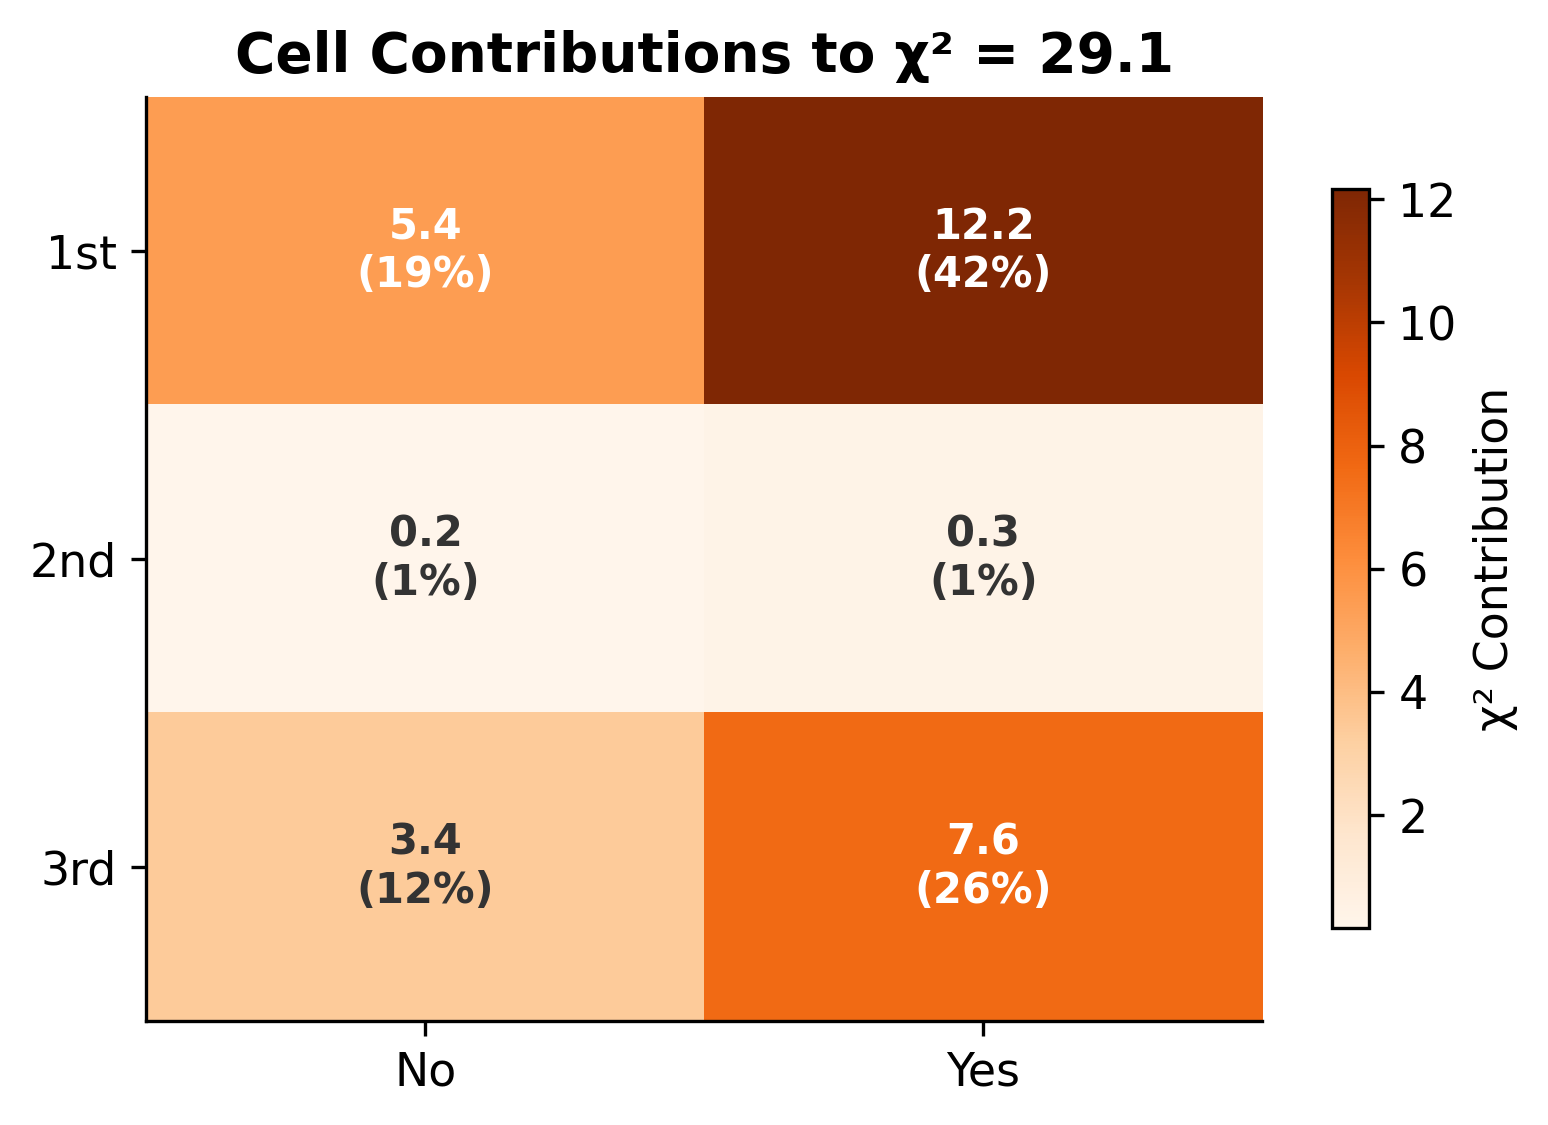
\includegraphics[width=0.58\textwidth]{m3_2_chi2_contrib.png}

\vspace{0.2cm}
\begin{columns}[T]
\begin{column}{0.48\textwidth}
\begin{itemize}
    \item Each cell contributes $r_{ij}^2$ to the total $\chi^2$
    \item Cells with large $r^2$ ``drive'' the significant result
    \item Annotate with both value and percentage of total $\chi^2$
    \item Identifies the \textbf{source} of the association
\end{itemize}
\end{column}
\begin{column}{0.48\textwidth}
\begin{exampleblock}{Data Insight}
    \scriptsize If one cell contributes 60\% of the total $\chi^2$, the ``significant association'' is really about that one cell. The rest of the table may be close to independence. Always decompose.
\end{exampleblock}
\end{column}
\end{columns}
\end{frame}

% ── 47 ──
\begin{frame}[fragile]{$\chi^2$ Contributions --- Code}\smark{47/300}
\begin{columns}[T]
\begin{column}{0.48\textwidth}
\begin{lstlisting}[style=Rstyle]
test <- chisq.test(ct)

# Cell contributions
contrib <- test$residuals^2
# Or
contrib <- (test$observed -
  test$expected)^2 /
  test$expected

# Percent of total
pct <- contrib / sum(contrib) * 100

# Visualize
corrplot(contrib, is.cor=FALSE,
  method="color",
  col=colorRampPalette(
    c("white","#B2182B"))(100))
\end{lstlisting}
\end{column}
\begin{column}{0.48\textwidth}
\begin{lstlisting}[style=Pystyle]
contrib = (ct.values - expected)**2\
    / expected
pct = contrib / contrib.sum() * 100

fig, ax = plt.subplots()
sns.heatmap(
    pd.DataFrame(contrib,
        index=ct.index,
        columns=ct.columns),
    annot=True, fmt=".1f",
    cmap="Oranges", ax=ax)
# Add percentage annotations
for i in range(3):
    for j in range(2):
        ax.text(j+0.5, i+0.7,
            f"({pct[i,j]:.0f}%)",
            ha="center", fontsize=8)
\end{lstlisting}
\end{column}
\end{columns}
\end{frame}

% ── 48 ──
\begin{frame}{Balloon Plots}
\smark{48/300}
\centering
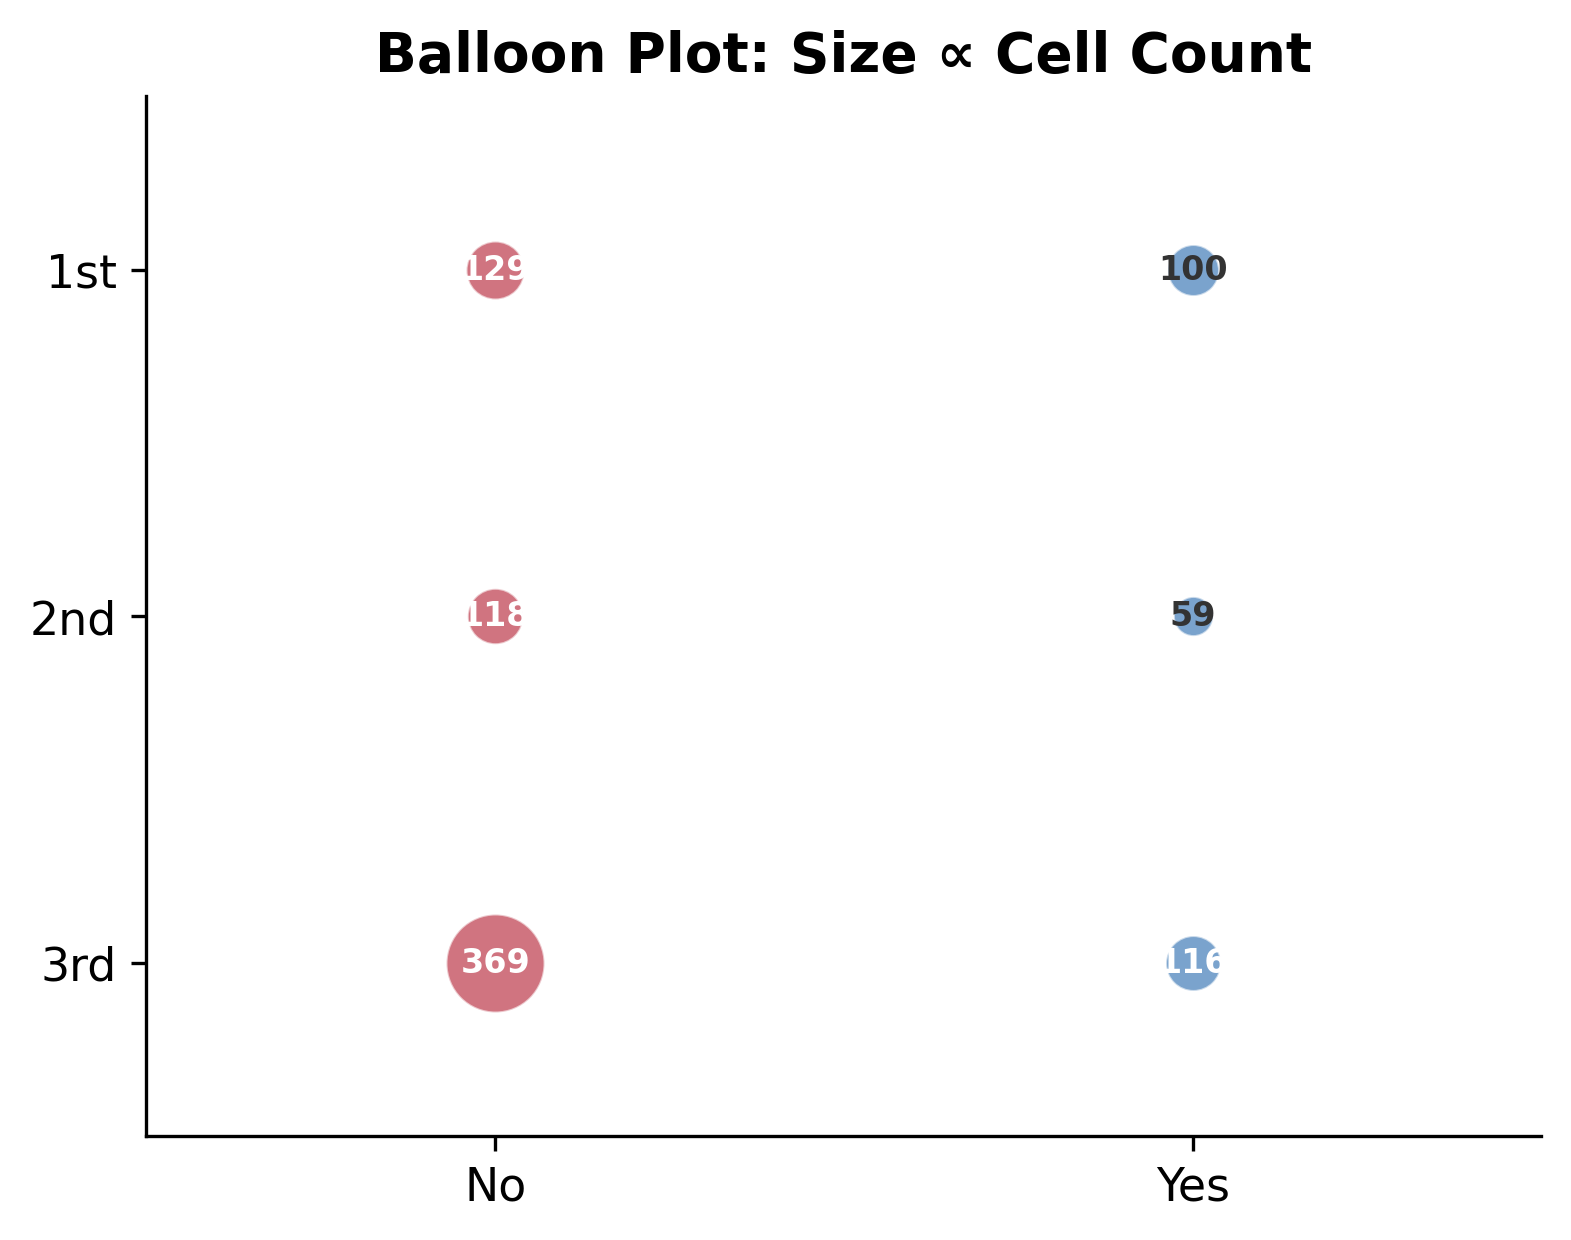
\includegraphics[width=0.55\textwidth]{m3_2_balloon.png}

\vspace{0.2cm}
\begin{columns}[T]
\begin{column}{0.48\textwidth}
\begin{itemize}
    \item Bubble size $\propto$ cell count
    \item Position encodes row $\times$ column cell
    \item Color can encode a third variable (e.g., residual sign)
    \item Works well for sparse tables where many cells are near-zero
\end{itemize}
\end{column}
\begin{column}{0.48\textwidth}
\begin{alertblock}{Pro-Tip}
    \scriptsize R: \texttt{ggpubr::ggballoonplot()} or \texttt{vcd::sieve()} (sieve diagrams are a variant). Python: manual \texttt{ax.scatter()} with size mapped to count. Balloon plots scale to larger tables than mosaics.
\end{alertblock}
\end{column}
\end{columns}
\end{frame}

% ── 49 ──
\begin{frame}[fragile]{Balloon Plot --- Code}\smark{49/300}
\begin{columns}[T]
\begin{column}{0.48\textwidth}
\begin{lstlisting}[style=Rstyle]
library(ggpubr)

# From cross-tab
ct_df <- as.data.frame(ct)
ggballoonplot(ct_df,
  x = "class", y = "survived",
  size = "Freq",
  fill = "Freq",
  ggtheme = theme_minimal())

# With residual coloring
ct_df$resid <- as.vector(
  chisq.test(ct)$residuals)
ggballoonplot(ct_df,
  x = "class", y = "survived",
  size = "Freq", fill = "resid")
\end{lstlisting}
\end{column}
\begin{column}{0.48\textwidth}
\begin{lstlisting}[style=Pystyle]
# Manual balloon in matplotlib
for i, cls in enumerate(classes):
    for j, surv in enumerate(survs):
        count = ct.loc[cls, surv]
        ax.scatter(j, 2-i,
            s=count * 1.5,
            color="#2166AC"
              if surv=="Yes"
              else "#B2182B",
            alpha=0.6)
        ax.text(j, 2-i, str(count),
            ha="center", va="center",
            fontsize=8, color="white")
ax.set_xticks([0,1])
ax.set_xticklabels(["No","Yes"])
\end{lstlisting}
\end{column}
\end{columns}
\end{frame}

% ── 50 ──
\begin{frame}{Sieve Diagrams}
\smark{50/300}
\begin{columns}[T]
\begin{column}{0.50\textwidth}
\begin{itemize}
    \item Like a mosaic, but cells have \textbf{equal area}
    \item Density of line hatching $\propto$ observed / expected ratio
    \item Dense hatching = more than expected; sparse = fewer
    \item Also called ``Parquet diagrams''
    \item Less common than mosaics but useful for detecting patterns in large tables
\end{itemize}
\end{column}
\begin{column}{0.47\textwidth}
\begin{alertblock}{Pro-Tip}
    \scriptsize R: \texttt{vcd::sieve(ct, shade=TRUE)}. No Python equivalent. Sieve diagrams are niche but effective --- they use \textbf{texture} instead of \textbf{color} to encode residuals, making them accessible for colorblind readers.
\end{alertblock}
\end{column}
\end{columns}
\end{frame}

% ── 51 ──
\begin{frame}{Fisher's Exact Test: When $\chi^2$ Fails}
\smark{51/300}
\begin{columns}[T]
\begin{column}{0.50\textwidth}
\begin{itemize}
    \item $\chi^2$ approximation breaks when expected counts $< 5$
    \item Fisher's exact test computes $p$ from the hypergeometric distribution
    \item No asymptotic approximation --- exact even for tiny tables
    \item Computationally expensive for large tables; use simulation
\end{itemize}
\end{column}
\begin{column}{0.47\textwidth}
\begin{alertblock}{Pro-Tip}
    \scriptsize R: \texttt{fisher.test(ct)} for $2 \times 2$; add \texttt{simulate.p.value=TRUE} for larger tables. Python: \texttt{scipy.stats.fisher\_exact()} for $2 \times 2$ only; use \texttt{chi2\_contingency} with \texttt{correction=True} for larger.
\end{alertblock}
\vspace{0.1cm}
\begin{exampleblock}{Data Insight}
    \scriptsize Visualize identically to $\chi^2$: mosaic + residual shading. The test changes but the display does not. Report ``Fisher's exact $p = 0.003$'' in the caption alongside the mosaic.
\end{exampleblock}
\end{column}
\end{columns}
\end{frame}

% ── 52 ──
\begin{frame}[fragile]{Fisher's Exact --- Code}\smark{52/300}
\begin{columns}[T]
\begin{column}{0.48\textwidth}
\begin{lstlisting}[style=Rstyle]
# 2x2 table
ct_2x2 <- matrix(c(100, 129,
                    116, 369),
                 nrow=2, byrow=TRUE)

fisher.test(ct_2x2)
# p-value, odds ratio, CI

# Larger tables (simulation)
fisher.test(ct,
  simulate.p.value = TRUE,
  B = 10000)

# Barnard's test (unconditional)
library(Barnard)
barnard.test(100, 129, 116, 369)
\end{lstlisting}
\end{column}
\begin{column}{0.48\textwidth}
\begin{lstlisting}[style=Pystyle]
from scipy.stats import fisher_exact

# 2x2 only
odds_ratio, p_value = fisher_exact(
    [[100, 129], [116, 369]])
print(f"OR={odds_ratio:.2f}, "
      f"p={p_value:.4f}")

# For larger tables: use chi2
# with Yates correction
chi2, p, dof, exp = \
    chi2_contingency(ct,
        correction=True)

# Or simulation-based
# (manual permutation approach)
\end{lstlisting}
\end{column}
\end{columns}
\end{frame}

% ── 53 ──
\begin{frame}{Standardized vs.\ Adjusted Residuals}
\smark{53/300}
\begin{columns}[T]
\begin{column}{0.50\textwidth}
\centering\small
\begin{tabular}{@{}ll@{}}
    \toprule
    \textbf{Type} & \textbf{Formula} \\
    \midrule
    Pearson   & $\frac{O-E}{\sqrt{E}}$ \\[6pt]
    Standardized & $\frac{O-E}{\sqrt{E(1-p_i)(1-p_j)}}$ \\[6pt]
    Adjusted  & Follows $N(0,1)$ under $H_0$ \\
    \bottomrule
\end{tabular}
\end{column}
\begin{column}{0.47\textwidth}
\begin{exampleblock}{Data Insight}
    \scriptsize Pearson residuals are not exactly standard normal. Adjusted (standardized) residuals correct for the marginal proportions and follow $N(0,1)$ under independence. Use $|r_{\text{adj}}| > 2$ as a cell-level significance threshold.
\end{exampleblock}
\vspace{0.1cm}
\begin{alertblock}{Pro-Tip}
    \scriptsize R: \texttt{chisq.test(ct)\$stdres} returns adjusted residuals. Python: compute manually as $r / \sqrt{(1 - p_i)(1 - p_j)}$ where $p_i, p_j$ are row and column marginal proportions.
\end{alertblock}
\end{column}
\end{columns}
\end{frame}

% ── 54 ──
\begin{frame}{Three-Way Tables: Conditional Association}
\smark{54/300}
\begin{columns}[T]
\begin{column}{0.50\textwidth}
\begin{itemize}
    \item Stratify by a third variable (e.g., sex)
    \item Run $\chi^2$ within each stratum
    \item Breslow--Day test: are the odds ratios homogeneous?
    \item Cochran--Mantel--Haenszel: pooled association controlling for the stratifier
    \item Visualize: faceted mosaics (one panel per stratum)
\end{itemize}
\end{column}
\begin{column}{0.47\textwidth}
\begin{alertblock}{Pro-Tip}
    \scriptsize R: \texttt{mantelhaen.test(ct\_3d)} for the CMH test. Visualize with \texttt{vcd::mosaic(survived \textasciitilde\ class | sex, data=titanic, shade=TRUE)} --- the \texttt{|} operator creates conditional panels.
\end{alertblock}
\vspace{0.1cm}
\begin{exampleblock}{Data Insight}
    \scriptsize Simpson's paradox strikes again: class $\times$ survival may reverse when stratified by sex. The conditional mosaic reveals this; the marginal mosaic hides it.
\end{exampleblock}
\end{column}
\end{columns}
\end{frame}

% ── 55 ──
\begin{frame}[fragile]{Conditional Mosaic --- Code}\smark{55/300}
\begin{columns}[T]
\begin{column}{0.48\textwidth}
\begin{lstlisting}[style=Rstyle]
library(vcd)

# Conditional on sex
mosaic(survived ~ class | sex,
  data = titanic,
  shade = TRUE)

# CMH test
ct_3d <- xtabs(~ class + survived
  + sex, data = titanic)
mantelhaen.test(ct_3d)

# Breslow-Day (homogeneity)
library(DescTools)
BreslowDayTest(ct_3d)
\end{lstlisting}
\end{column}
\begin{column}{0.48\textwidth}
\begin{lstlisting}[style=Pystyle]
# Faceted mosaics: one per stratum
fig, axes = plt.subplots(1, 2,
    figsize=(12, 5))
for ax, sx in zip(axes,
    ["Female","Male"]):
    sub = titanic[titanic.sex==sx]
    ct_sub = pd.crosstab(
        sub["class"],
        sub["survived"])
    # Draw mosaic on ax
    # (manual rectangle approach)
    ax.set_title(sx)

# CMH test (not in scipy)
# Use rpy2 or cochran_q from
# statsmodels for repeated measures
\end{lstlisting}
\end{column}
\end{columns}
\end{frame}

% ── 56 ──
\begin{frame}{Reporting $\chi^2$ Results Visually}
\smark{56/300}
\centering\small
\begin{tabular}{@{}ll@{}}
    \toprule
    \textbf{Show} & \textbf{How} \\
    \midrule
    Joint distribution    & Mosaic plot (area $\propto$ frequency) \\
    Deviation direction   & Residual shading (blue/red) \\
    Deviation magnitude   & Residual value annotation in cells \\
    Which cells drive it  & $\chi^2$ contribution heatmap \\
    Effect size           & Cramér's $V$ (in caption) \\
    Sample sizes          & Marginal totals on mosaic labels \\
    Significance          & $\chi^2$, $df$, $p$ in caption \\
    \bottomrule
\end{tabular}

\vspace{0.3cm}
\begin{exampleblock}{Data Insight}
    \scriptsize A residual-shaded mosaic with cell counts, Cramér's $V$ in the subtitle, and $\chi^2(2) = 47.3$, $p < 0.001$ in the caption gives the reader \textbf{everything} in one figure.
\end{exampleblock}
\end{frame}

% ── 57 ──
\begin{frame}{Association Visualization Decision Guide}
\smark{57/300}
\centering\small
\begin{tabular}{@{}lll@{}}
    \toprule
    \textbf{Task} & \textbf{Plot} & \textbf{R Package} \\
    \midrule
    Joint distribution + association     & Mosaic (shaded)      & \texttt{vcd::mosaic(shade=TRUE)} \\
    Residual direction only              & Association plot      & \texttt{vcd::assoc()} \\
    Cell counts as size                  & Balloon plot          & \texttt{ggpubr::ggballoonplot()} \\
    Residual heatmap (simple)            & Tile plot             & \texttt{corrplot()} on residuals \\
    Which cells drive $\chi^2$?          & Contribution heatmap  & Manual from \texttt{chisq.test()} \\
    $2 \times 2$ odds ratio              & Forest plot           & \texttt{epitools::oddsratio()} \\
    Conditional (3-way)                  & Faceted mosaic        & \texttt{mosaic(\textasciitilde\ | z)} \\
    Effect size scale                    & Cramér's $V$ bar      & Manual \\
    \bottomrule
\end{tabular}
\end{frame}

% ── 58 ──
\begin{frame}{Common Mistakes in Categorical Association}
\smark{58/300}
\centering\small
\begin{tabular}{@{}ll@{}}
    \toprule
    \textbf{Mistake} & \textbf{Fix} \\
    \midrule
    Report $\chi^2$ without effect size        & Always report Cramér's $V$ or odds ratio \\
    $\chi^2$ with expected $< 5$               & Use Fisher's exact test \\
    Ignore which cells drive the result        & Examine Pearson residuals per cell \\
    Use bar chart for association               & Use mosaic with residual shading \\
    No conditioning on confounders             & Stratified / conditional mosaics \\
    Interpret $\chi^2$ as causal               & It tests association, not causation \\
    \bottomrule
\end{tabular}
\end{frame}

% ── 59 ──
\begin{frame}{$\chi^2$ Assumptions and Alternatives}
\smark{59/300}
\centering\small
\begin{tabular}{@{}lll@{}}
    \toprule
    \textbf{Issue} & \textbf{Test} & \textbf{When} \\
    \midrule
    Standard test           & Pearson $\chi^2$            & Expected $\geq 5$ in all cells \\
    Sparse cells            & Fisher's exact              & Any cell $< 5$ expected \\
    $2 \times 2$, small $n$ & Barnard's test              & Most powerful unconditional \\
    Ordinal variables       & Linear-by-linear            & Both variables ordinal \\
    Repeated measures       & McNemar's test              & Paired $2 \times 2$ \\
    Stratified              & CMH test                    & Control for a confounder \\
    Goodness-of-fit         & $\chi^2$ one-sample         & Compare to fixed proportions \\
    \bottomrule
\end{tabular}

\vspace{0.3cm}
\begin{alertblock}{Pro-Tip}
    \scriptsize For ordinal $\times$ ordinal tables, use the linear-by-linear association test (\texttt{vcd::assocstats()}) or Kendall's $\tau$ rather than $\chi^2$, which ignores order.
\end{alertblock}
\end{frame}

% ── 60 ──
\begin{frame}{Module 3.2 --- Key Takeaways}\smark{60/300}
\begin{enumerate}
    \item \textbf{Residual-shaded mosaics} integrate the $\chi^2$ test result directly into the display.
    \item \textbf{Pearson residuals} show \emph{where} the association lives: which cells deviate from independence.
    \item \textbf{Cramér's $V$} is the effect size --- always report it alongside $\chi^2$ and $p$.
    \item \textbf{Cell contributions} decompose the global $\chi^2$ into per-cell sources.
    \item \textbf{Fisher's exact test} when expected counts $< 5$.
    \item \textbf{Conditional mosaics} expose confounding and Simpson's paradox in categorical data.
\end{enumerate}
\end{frame}

% ── 61 ──
\begin{frame}{}\smark{61/300}
\centering\vspace{1.5cm}
{\Large\textbf{Module 3.2 Complete}}\\[0.5cm]
You can now test and visualize categorical association with residual-shaded mosaics, association plots, $\chi^2$ decompositions, and Cramér's $V$ --- and know when to use Fisher's exact or conditional analysis.\\[0.5cm]
\textbf{Next:} Module 3.3 --- Alluvial, Sankey, and Flow Diagrams.
\end{frame}

% ═══════════════════════════════════════════════════════
%  MODULE 3.3 — Alluvial, Sankey, and Flow Diagrams
% ═══════════════════════════════════════════════════════
\section{Module 3.3 --- Alluvial, Sankey, and Flow Diagrams}

% ── 62 ──
\begin{frame}{Module 3.3 --- Roadmap}\smark{62/300}
\begin{enumerate}
    \item Alluvial diagrams: multi-variable categorical flow
    \item Sankey diagrams: quantitative flow networks
    \item Parallel sets: the categorical parallel coordinates
    \item Bump charts: rank changes over time
    \item Slope charts: before/after comparisons
    \item UpSet plots: set intersection beyond Venn
    \item When flows mislead: design principles
    \item Package ecosystem for flow visualizations
\end{enumerate}
\end{frame}

% ── 63 ──
\begin{frame}{Alluvial Diagrams}
\smark{63/300}
\centering
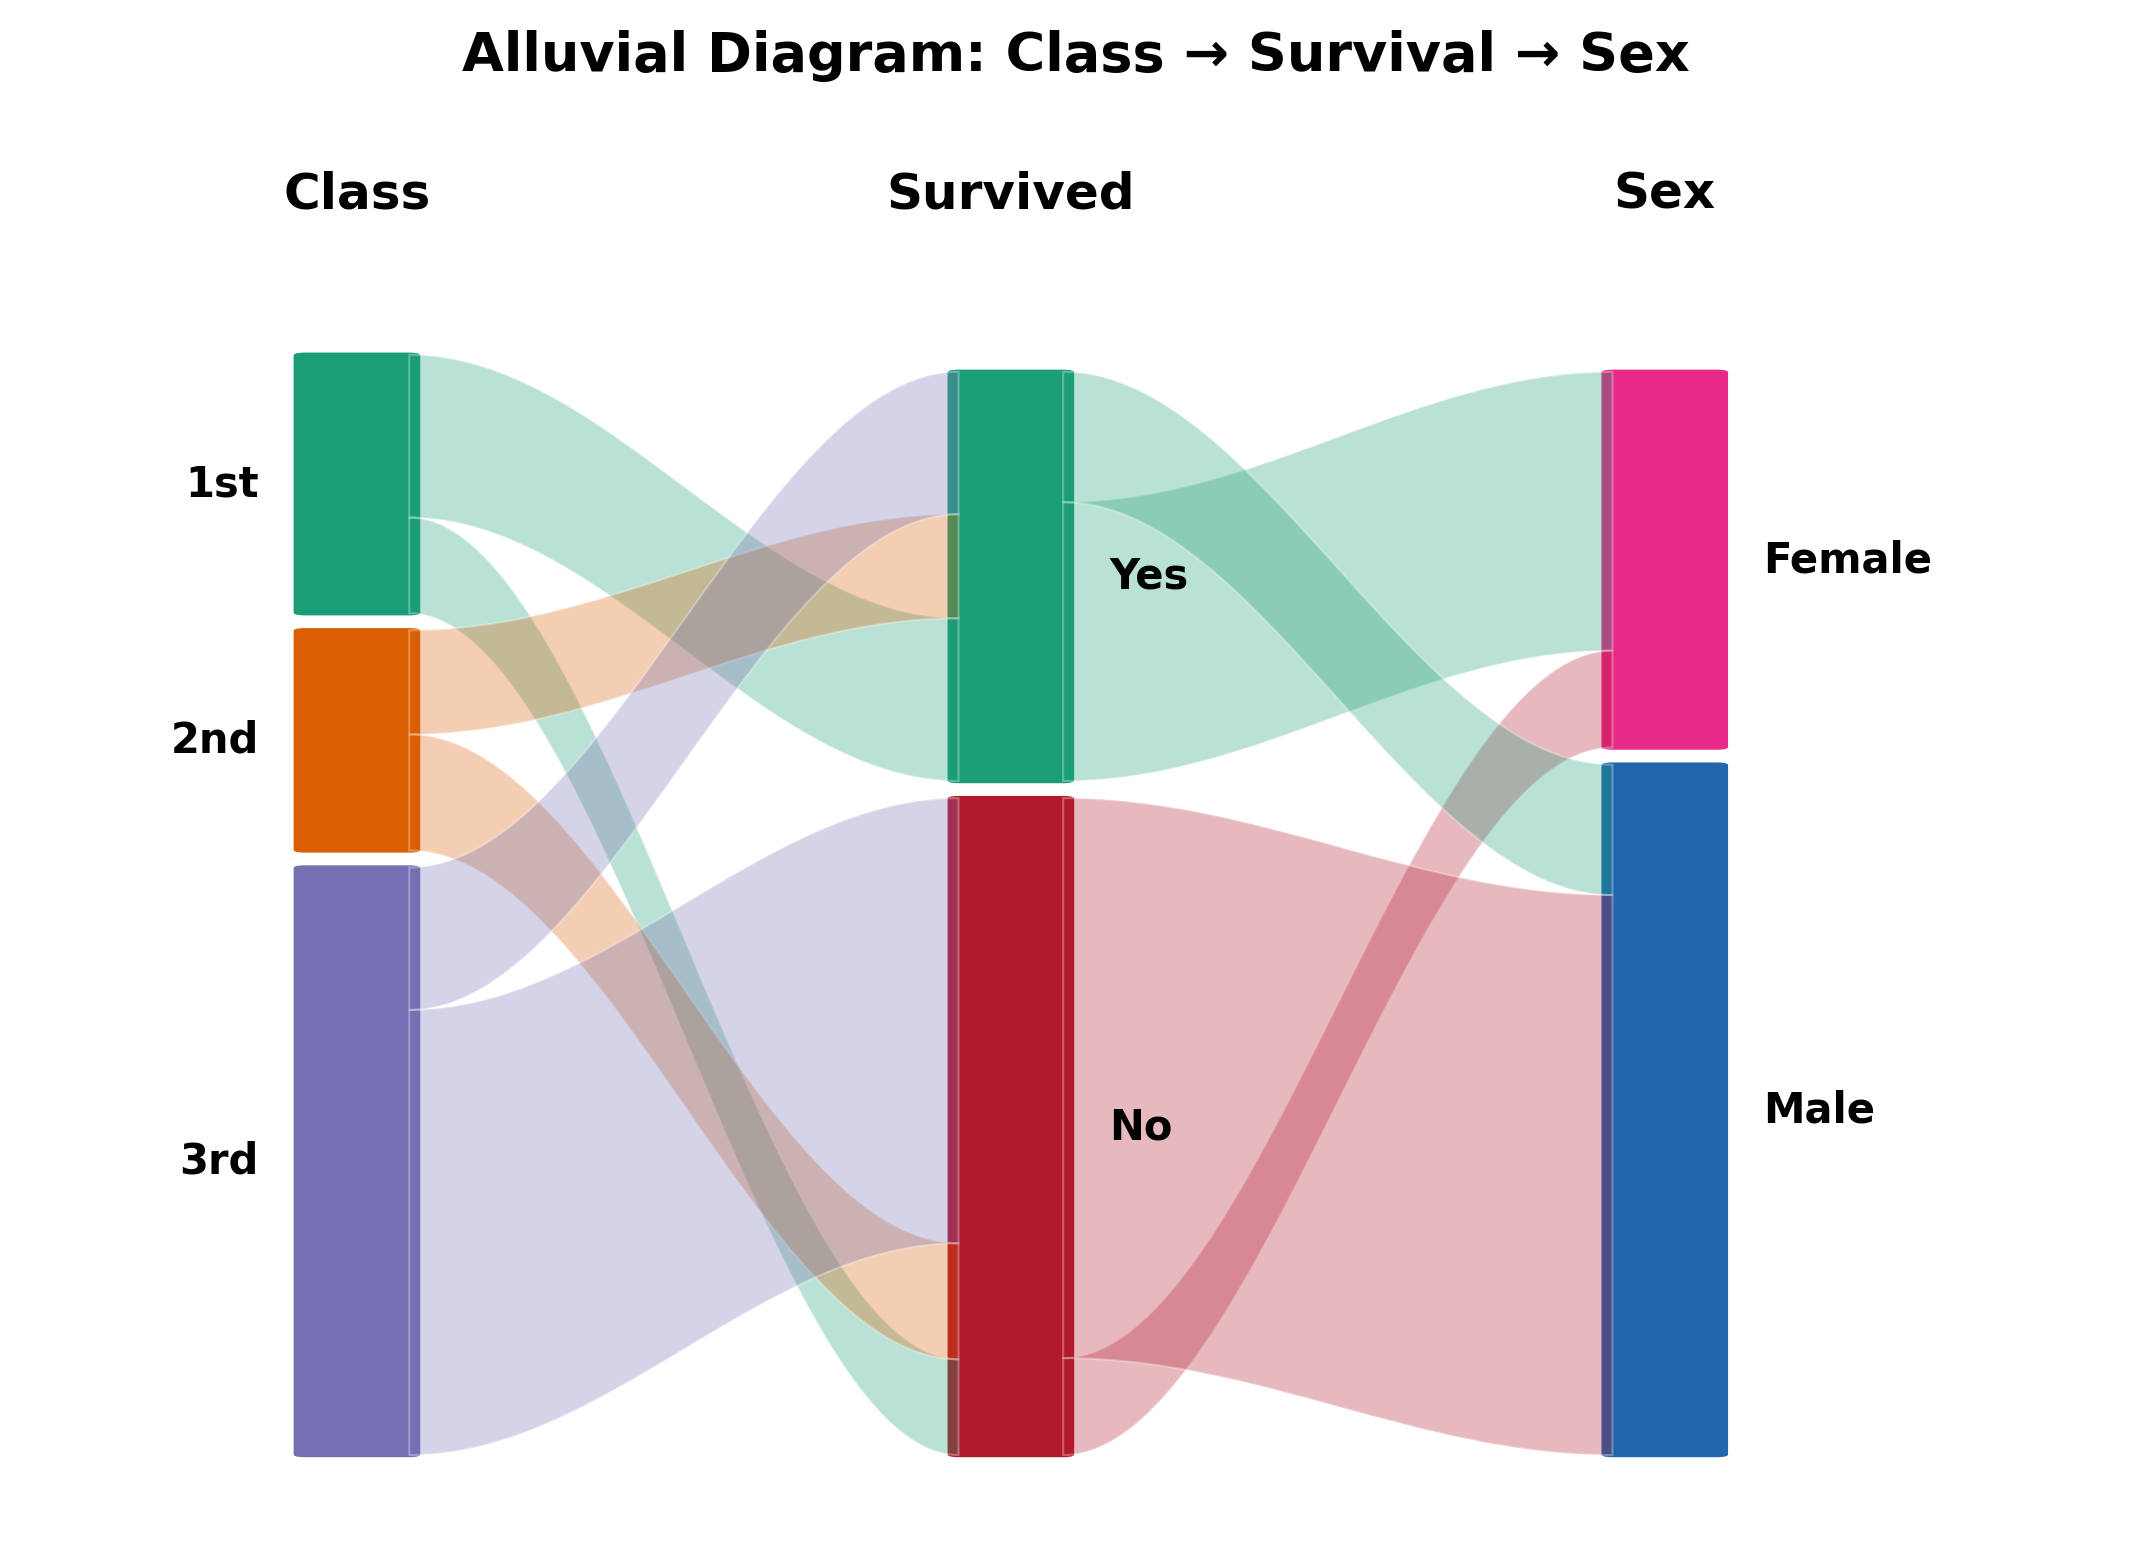
\includegraphics[width=0.72\textwidth]{m3_3_alluvial.png}

\vspace{0.2cm}
\begin{columns}[T]
\begin{column}{0.48\textwidth}
\begin{itemize}
    \item Vertical bars = categorical variables (axes)
    \item Curved bands (strata) = flows between categories
    \item Band width $\propto$ count or proportion
    \item Shows how observations \textbf{partition} across multiple categorical variables
\end{itemize}
\end{column}
\begin{column}{0.48\textwidth}
\begin{exampleblock}{Data Insight}
    \scriptsize The thick green band from 3rd class to ``No'' (died) dominates the display: most 3rd-class passengers perished. The thin bands connecting 1st class to ``Yes'' to ``Female'' trace the ``women and children first'' effect.
\end{exampleblock}
\end{column}
\end{columns}
\end{frame}

% ── 64 ──
\begin{frame}{Alluvial vs.\ Sankey: What's the Difference?}
\smark{64/300}
\centering\small
\begin{tabular}{@{}lll@{}}
    \toprule
    \textbf{Feature} & \textbf{Alluvial} & \textbf{Sankey} \\
    \midrule
    Axes         & Categorical variables (parallel) & Nodes in a network \\
    Bands        & Partition of the same observations & Flows of quantity between nodes \\
    Conservation & Each observation appears once     & Flow is conserved (in = out) \\
    Typical data & Survey responses, patient pathways & Energy, budget, material flows \\
    R package    & \texttt{ggalluvial}               & \texttt{networkD3}, \texttt{ggsankey} \\
    Python       & \texttt{plotly} (Sankey), manual   & \texttt{plotly.graph\_objects.Sankey} \\
    \bottomrule
\end{tabular}

\vspace{0.3cm}
\begin{alertblock}{Pro-Tip}
    \scriptsize In practice, the terms are often used interchangeably. The key distinction: alluvial diagrams show \textbf{the same entities} flowing across categorical axes. Sankey diagrams show \textbf{quantities} flowing between nodes (energy, money, material).
\end{alertblock}
\end{frame}

% ── 65 ──
\begin{frame}[fragile]{Alluvial --- \Rlang}\smark{65/300}
\begin{columns}[T]
\begin{column}{0.55\textwidth}
\begin{lstlisting}[style=Rstyle]
library(ggalluvial)

ggplot(titanic,
  aes(axis1 = class,
      axis2 = survived,
      axis3 = sex)) +
  geom_alluvium(
    aes(fill = class),
    alpha = 0.4) +
  geom_stratum(
    fill = "grey90",
    color = "white") +
  geom_text(
    stat = "stratum",
    aes(label = after_stat(
      stratum))) +
  scale_fill_manual(
    values=c("#1B9E77","#D95F02",
             "#7570B3")) +
  theme_void()
\end{lstlisting}
\end{column}
\begin{column}{0.42\textwidth}
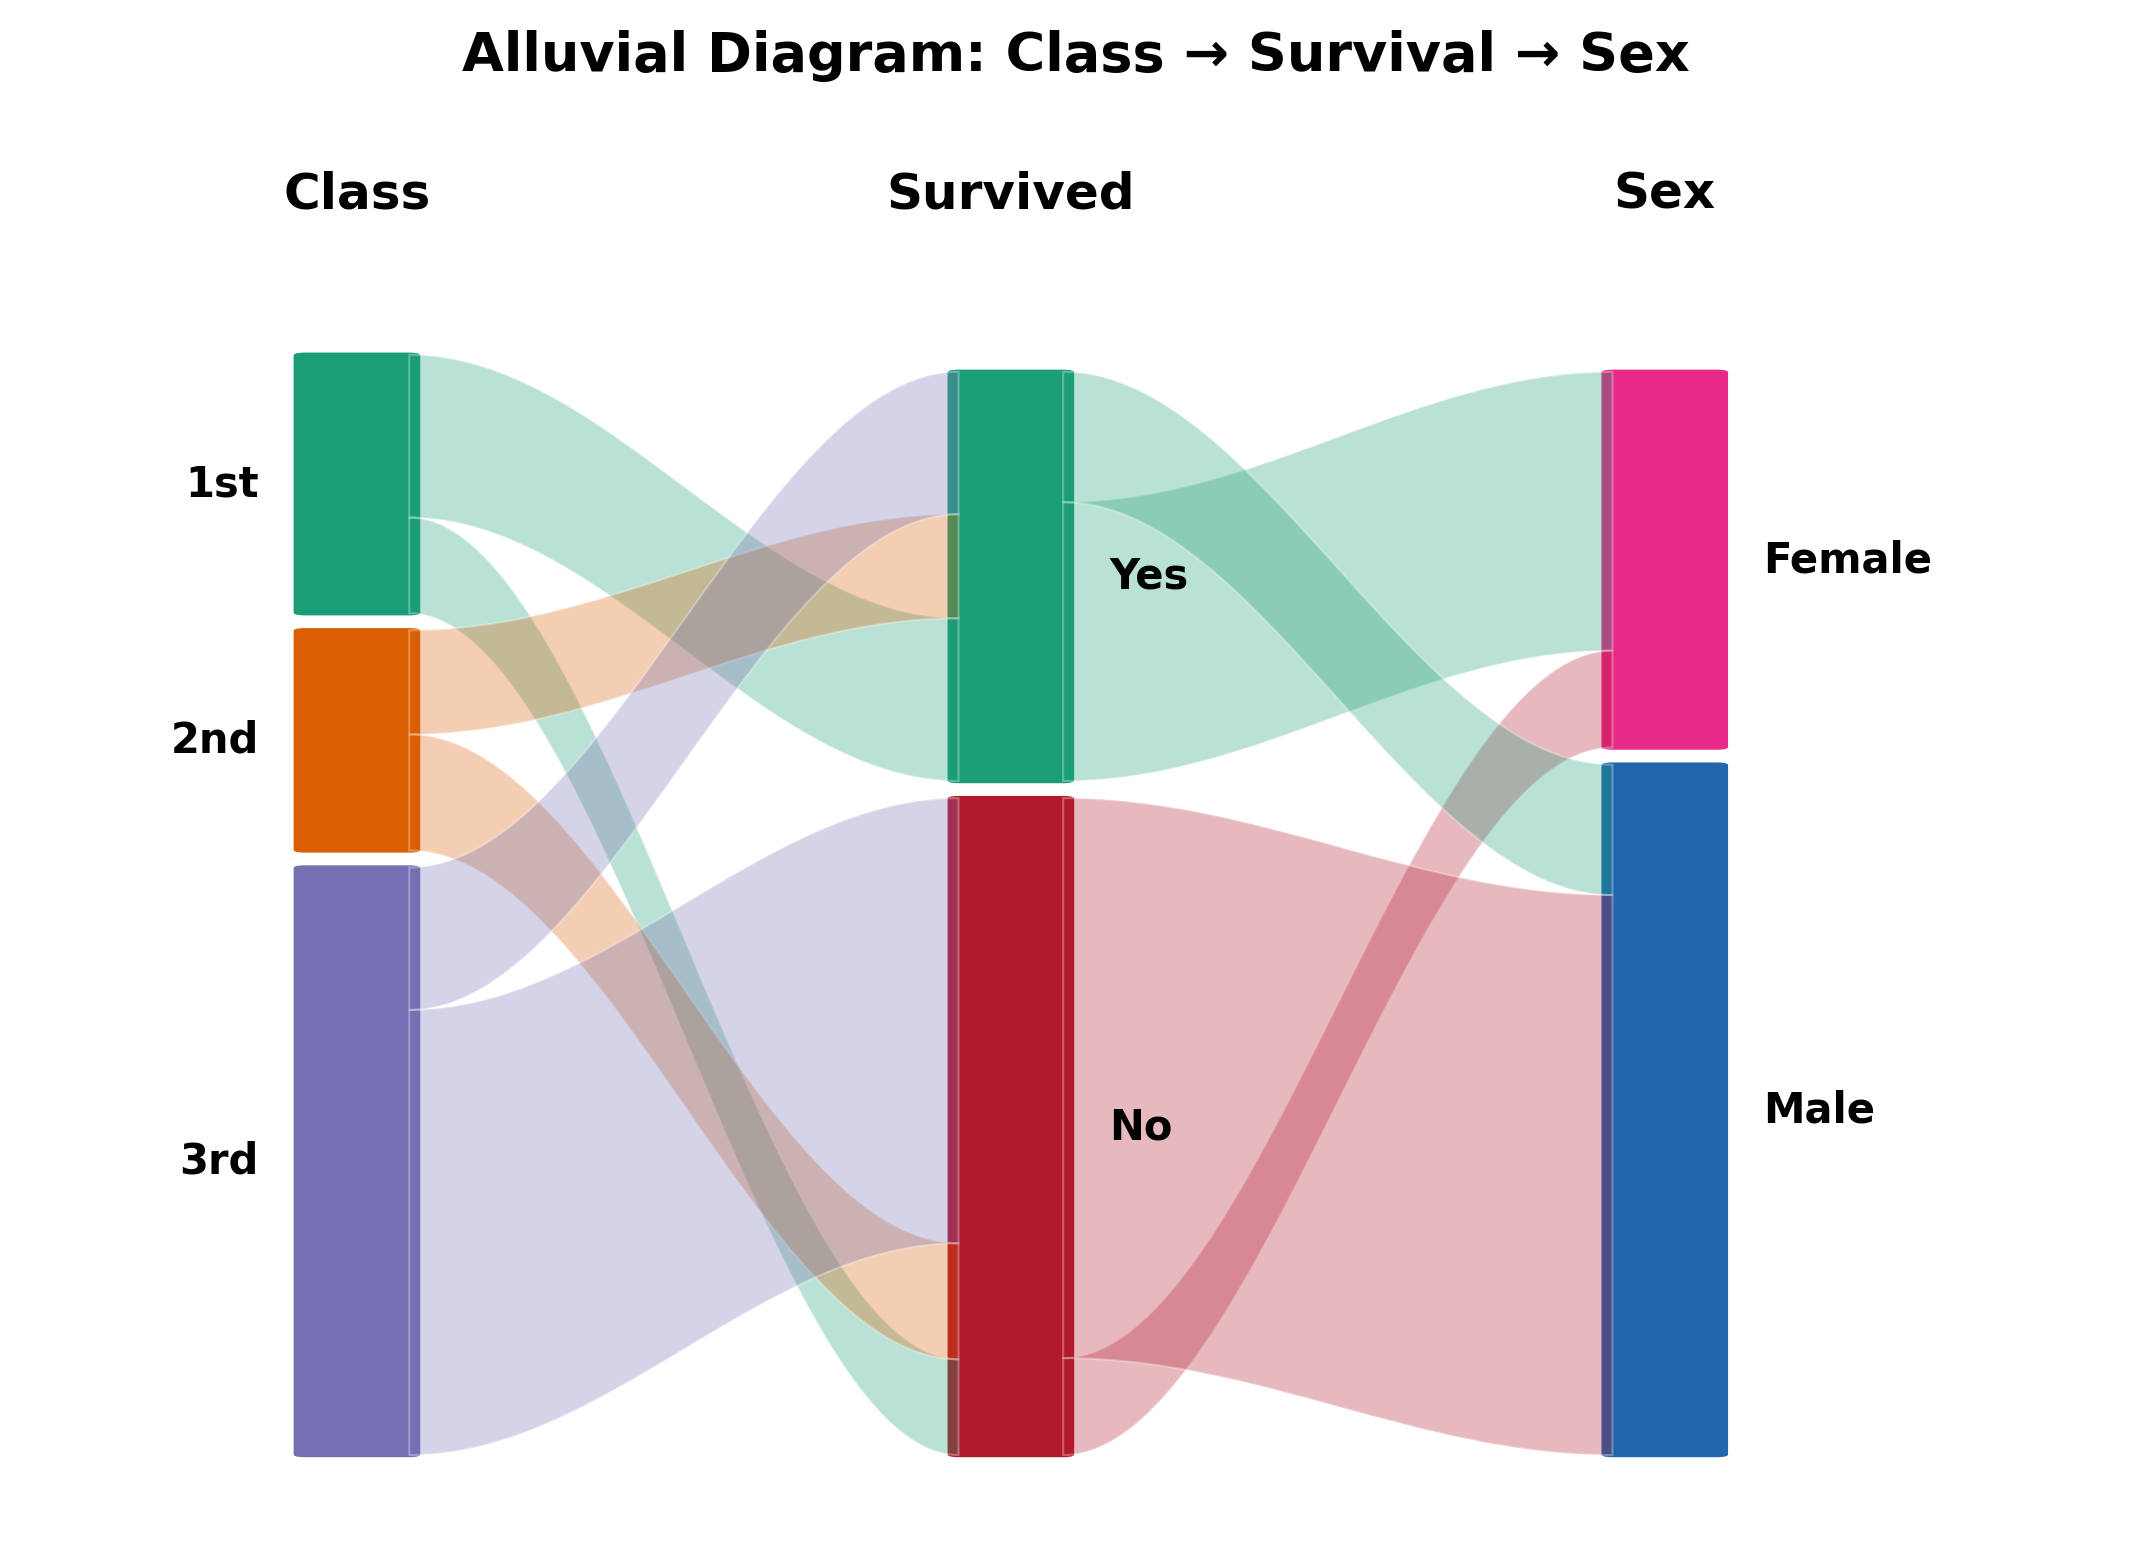
\includegraphics[width=\textwidth]{m3_3_alluvial.png}
\begin{alertblock}{Pro-Tip}
    \scriptsize \texttt{ggalluvial} requires data in ``alluvial form'' (one row per unique combination + frequency) or ``lode form'' (one row per observation). Use \texttt{to\_lodes\_form()} to convert.
\end{alertblock}
\end{column}
\end{columns}
\end{frame}

% ── 66 ──
\begin{frame}[fragile]{Alluvial --- \Python}\smark{66/300}
\begin{columns}[T]
\begin{column}{0.55\textwidth}
\begin{lstlisting}[style=Pystyle]
import plotly.graph_objects as go

# Plotly Sankey (alluvial-style)
fig = go.Figure(go.Sankey(
    node=dict(
        label=["1st","2nd","3rd",
               "Yes","No",
               "Female","Male"],
        color=[...]),
    link=dict(
        source=[0,0,1,1,2,2, ...],
        target=[3,4,3,4,3,4, ...],
        value=[136,80,87,97, ...],
        color=[...])
))
fig.update_layout(
    title="Alluvial: Titanic")
fig.show()

# Static: manual matplotlib
# (as in the plot generation code)
\end{lstlisting}
\end{column}
\begin{column}{0.42\textwidth}
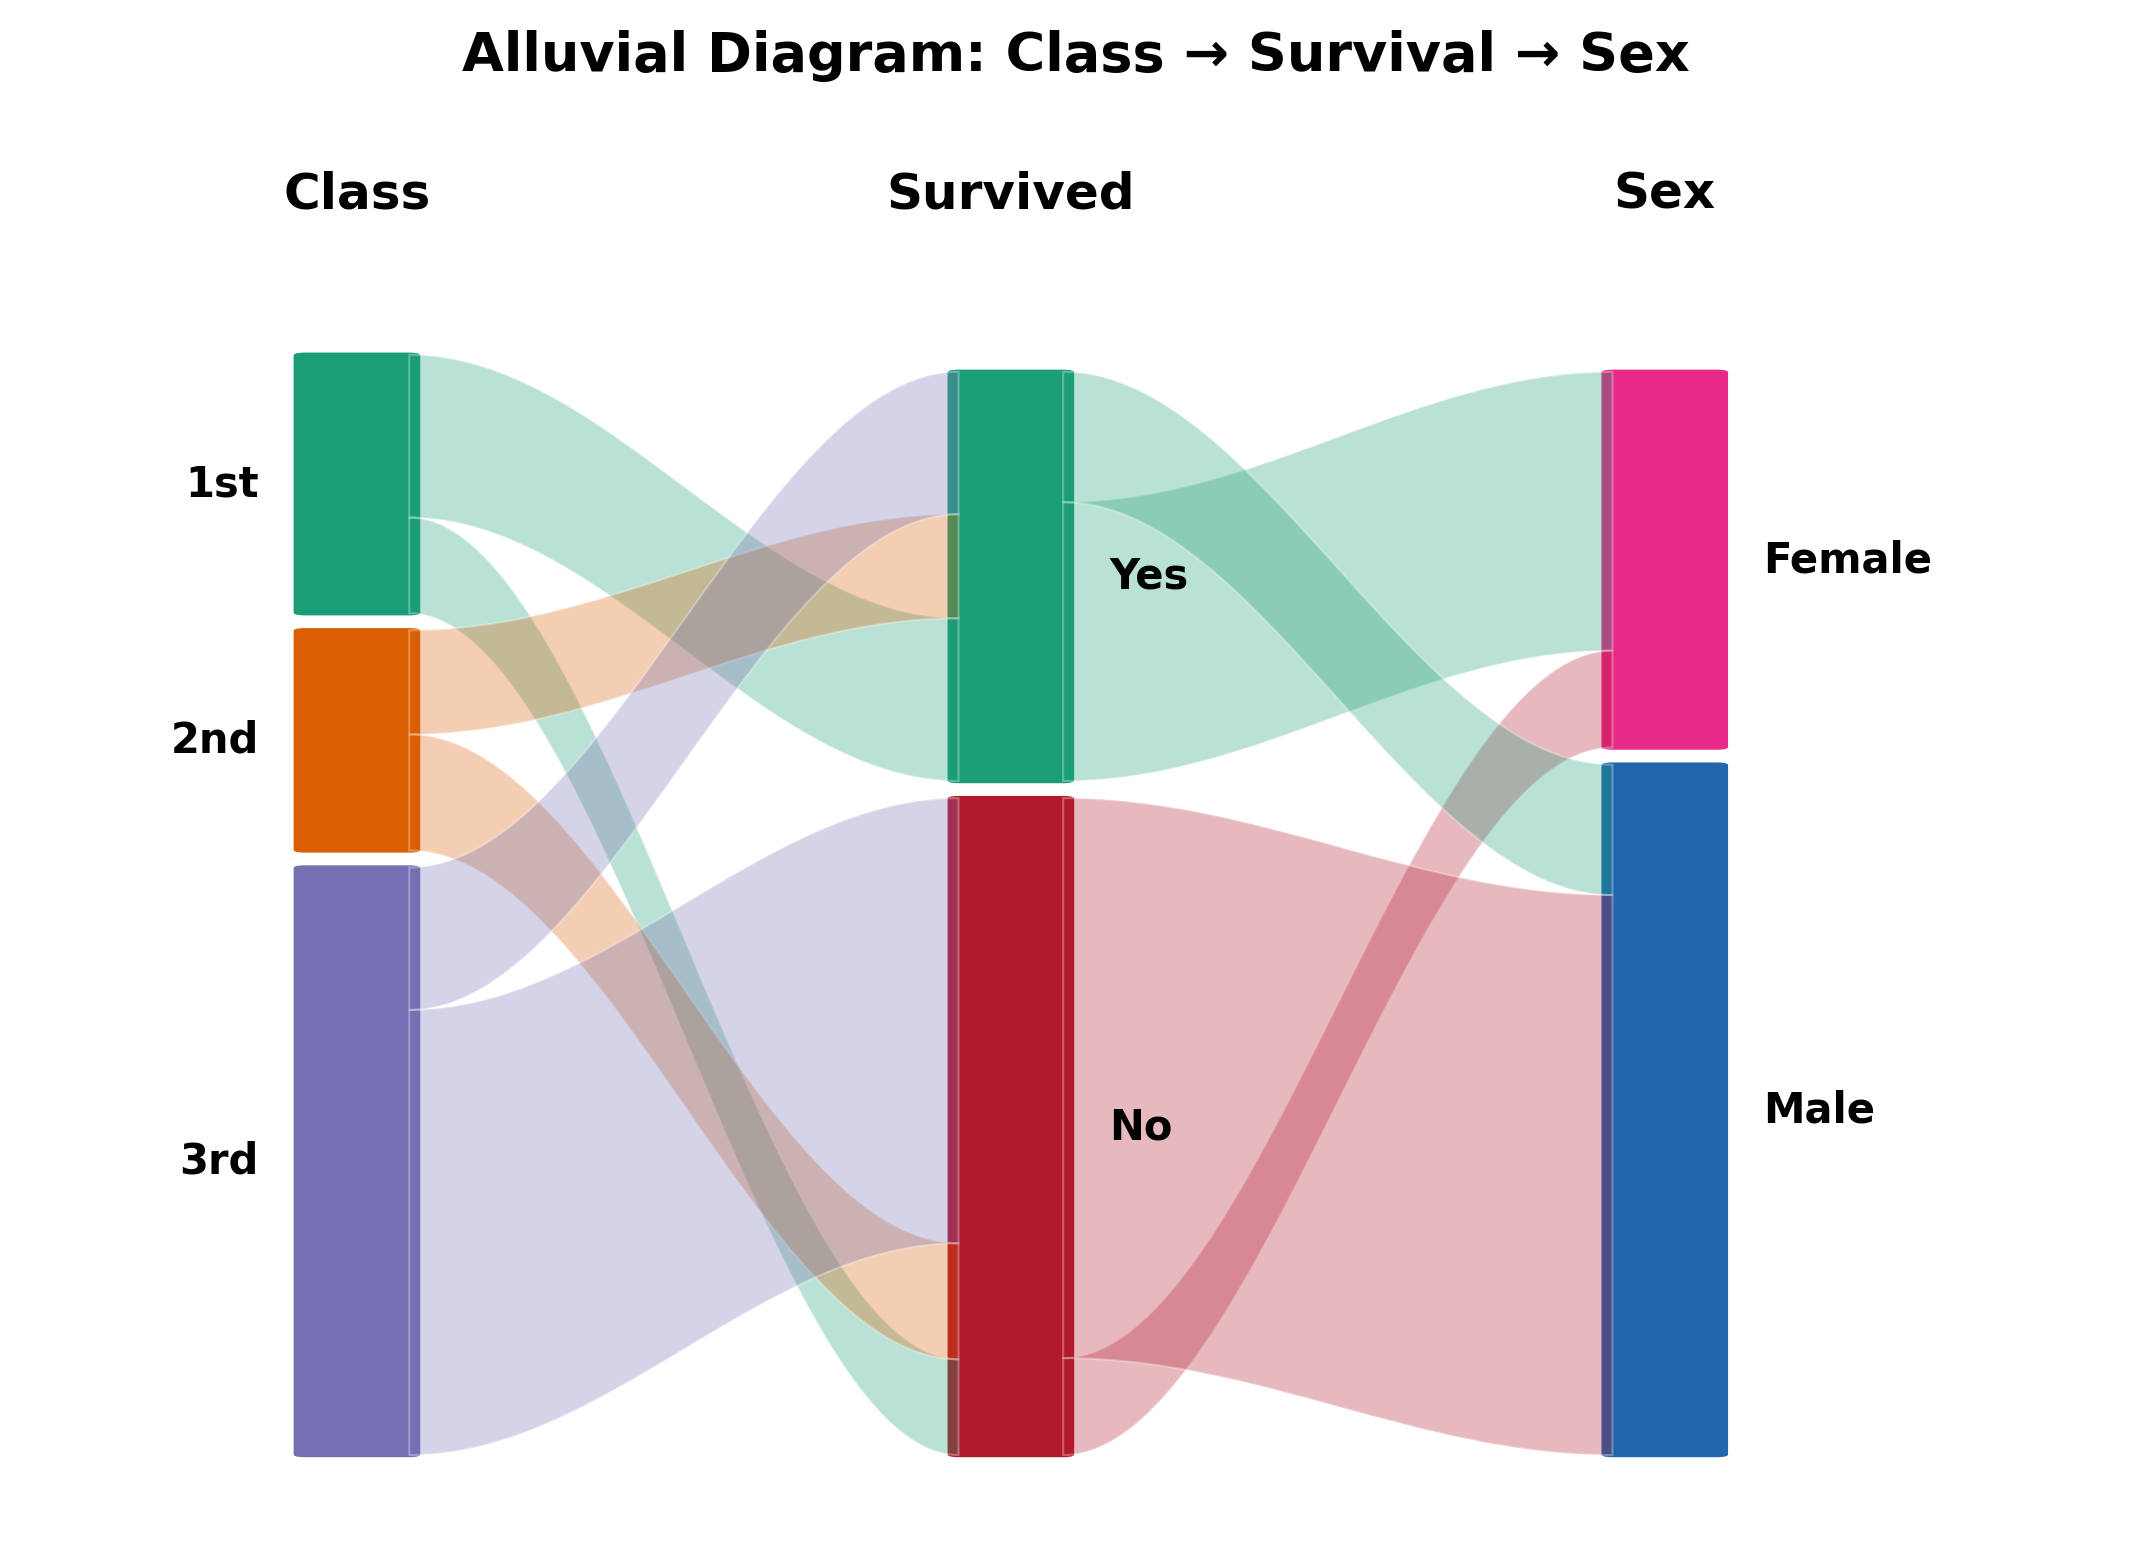
\includegraphics[width=\textwidth]{m3_3_alluvial.png}
\begin{exampleblock}{Data Insight}
    \scriptsize Plotly's \texttt{go.Sankey()} is the most practical Python option --- it produces interactive alluvial/Sankey diagrams with hover tooltips. For static publication figures, build manually with matplotlib paths.
\end{exampleblock}
\end{column}
\end{columns}
\end{frame}

% ── 67 ──
\begin{frame}{Sankey Diagrams: Quantitative Flows}
\smark{67/300}
\centering
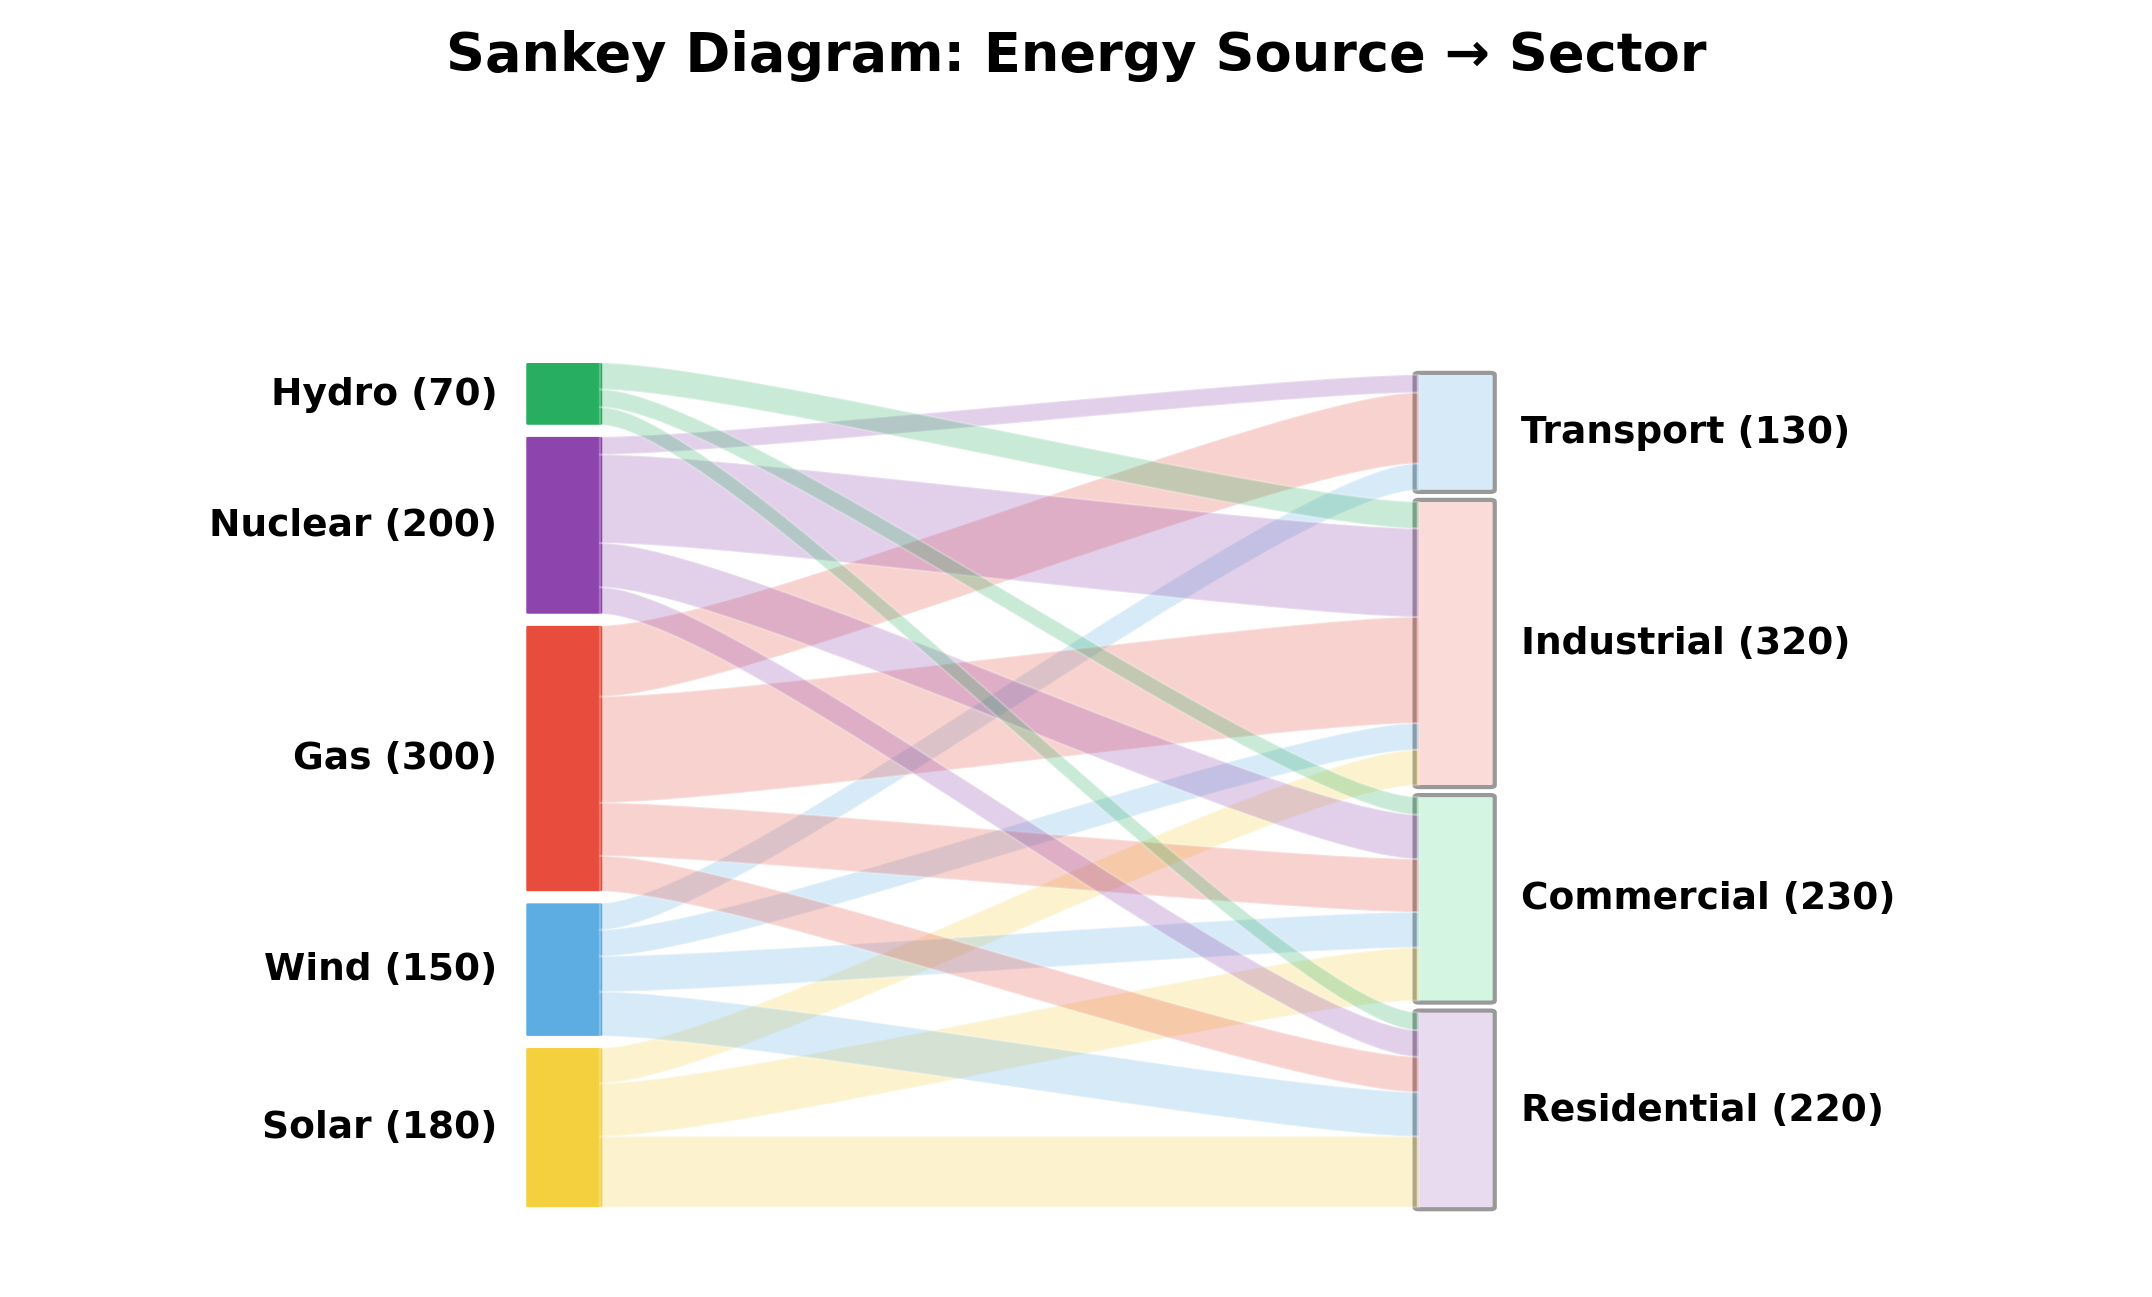
\includegraphics[width=0.72\textwidth]{m3_3_sankey.png}

\vspace{0.2cm}
\begin{columns}[T]
\begin{column}{0.48\textwidth}
\begin{itemize}
    \item Nodes = sources and destinations
    \item Links = flow of quantity (energy, money, patients)
    \item Width $\propto$ flow magnitude
    \item Flow is \textbf{conserved}: total in = total out
    \item Classic use: energy balance diagrams (LLNL)
\end{itemize}
\end{column}
\begin{column}{0.48\textwidth}
\begin{exampleblock}{Data Insight}
    \scriptsize Gas is the largest source and feeds all sectors, especially Industrial. Solar and Wind primarily serve Residential and Commercial. The visual immediately reveals the dominant pathways and bottlenecks.
\end{exampleblock}
\end{column}
\end{columns}
\end{frame}

% ── 68 ──
\begin{frame}[fragile]{Sankey --- Code}\smark{68/300}
\begin{columns}[T]
\begin{column}{0.48\textwidth}
\begin{lstlisting}[style=Rstyle]
library(networkD3)

# Node data frame
nodes <- data.frame(
  name=c("Solar","Wind","Gas",
    "Nuclear","Hydro",
    "Residential","Commercial",
    "Industrial","Transport"))

# Link data frame
links <- data.frame(
  source=c(0,0,0,1,1,1,...),
  target=c(5,6,7,5,6,7,...),
  value=c(80,60,40,50,40,30,...))

sankeyNetwork(Links=links,
  Nodes=nodes, Source="source",
  Target="target", Value="value",
  NodeID="name", fontSize=12)
\end{lstlisting}
\end{column}
\begin{column}{0.48\textwidth}
\begin{lstlisting}[style=Pystyle]
import plotly.graph_objects as go

fig = go.Figure(go.Sankey(
    node=dict(
        label=node_names,
        color=node_colors),
    link=dict(
        source=source_indices,
        target=target_indices,
        value=flow_values,
        color=link_colors)
))
fig.update_layout(
    title="Energy Flow")
fig.write_html("sankey.html")
fig.write_image("sankey.png")
\end{lstlisting}
\vspace{0.1cm}
\begin{alertblock}{Pro-Tip}
    \scriptsize \texttt{networkD3::sankeyNetwork()} produces interactive HTML. \texttt{plotly} does the same in Python. For static PDF output, use \texttt{fig.write\_image()} (requires kaleido).
\end{alertblock}
\end{column}
\end{columns}
\end{frame}

% ── 69 ──
\begin{frame}{Parallel Sets}
\smark{69/300}
\centering
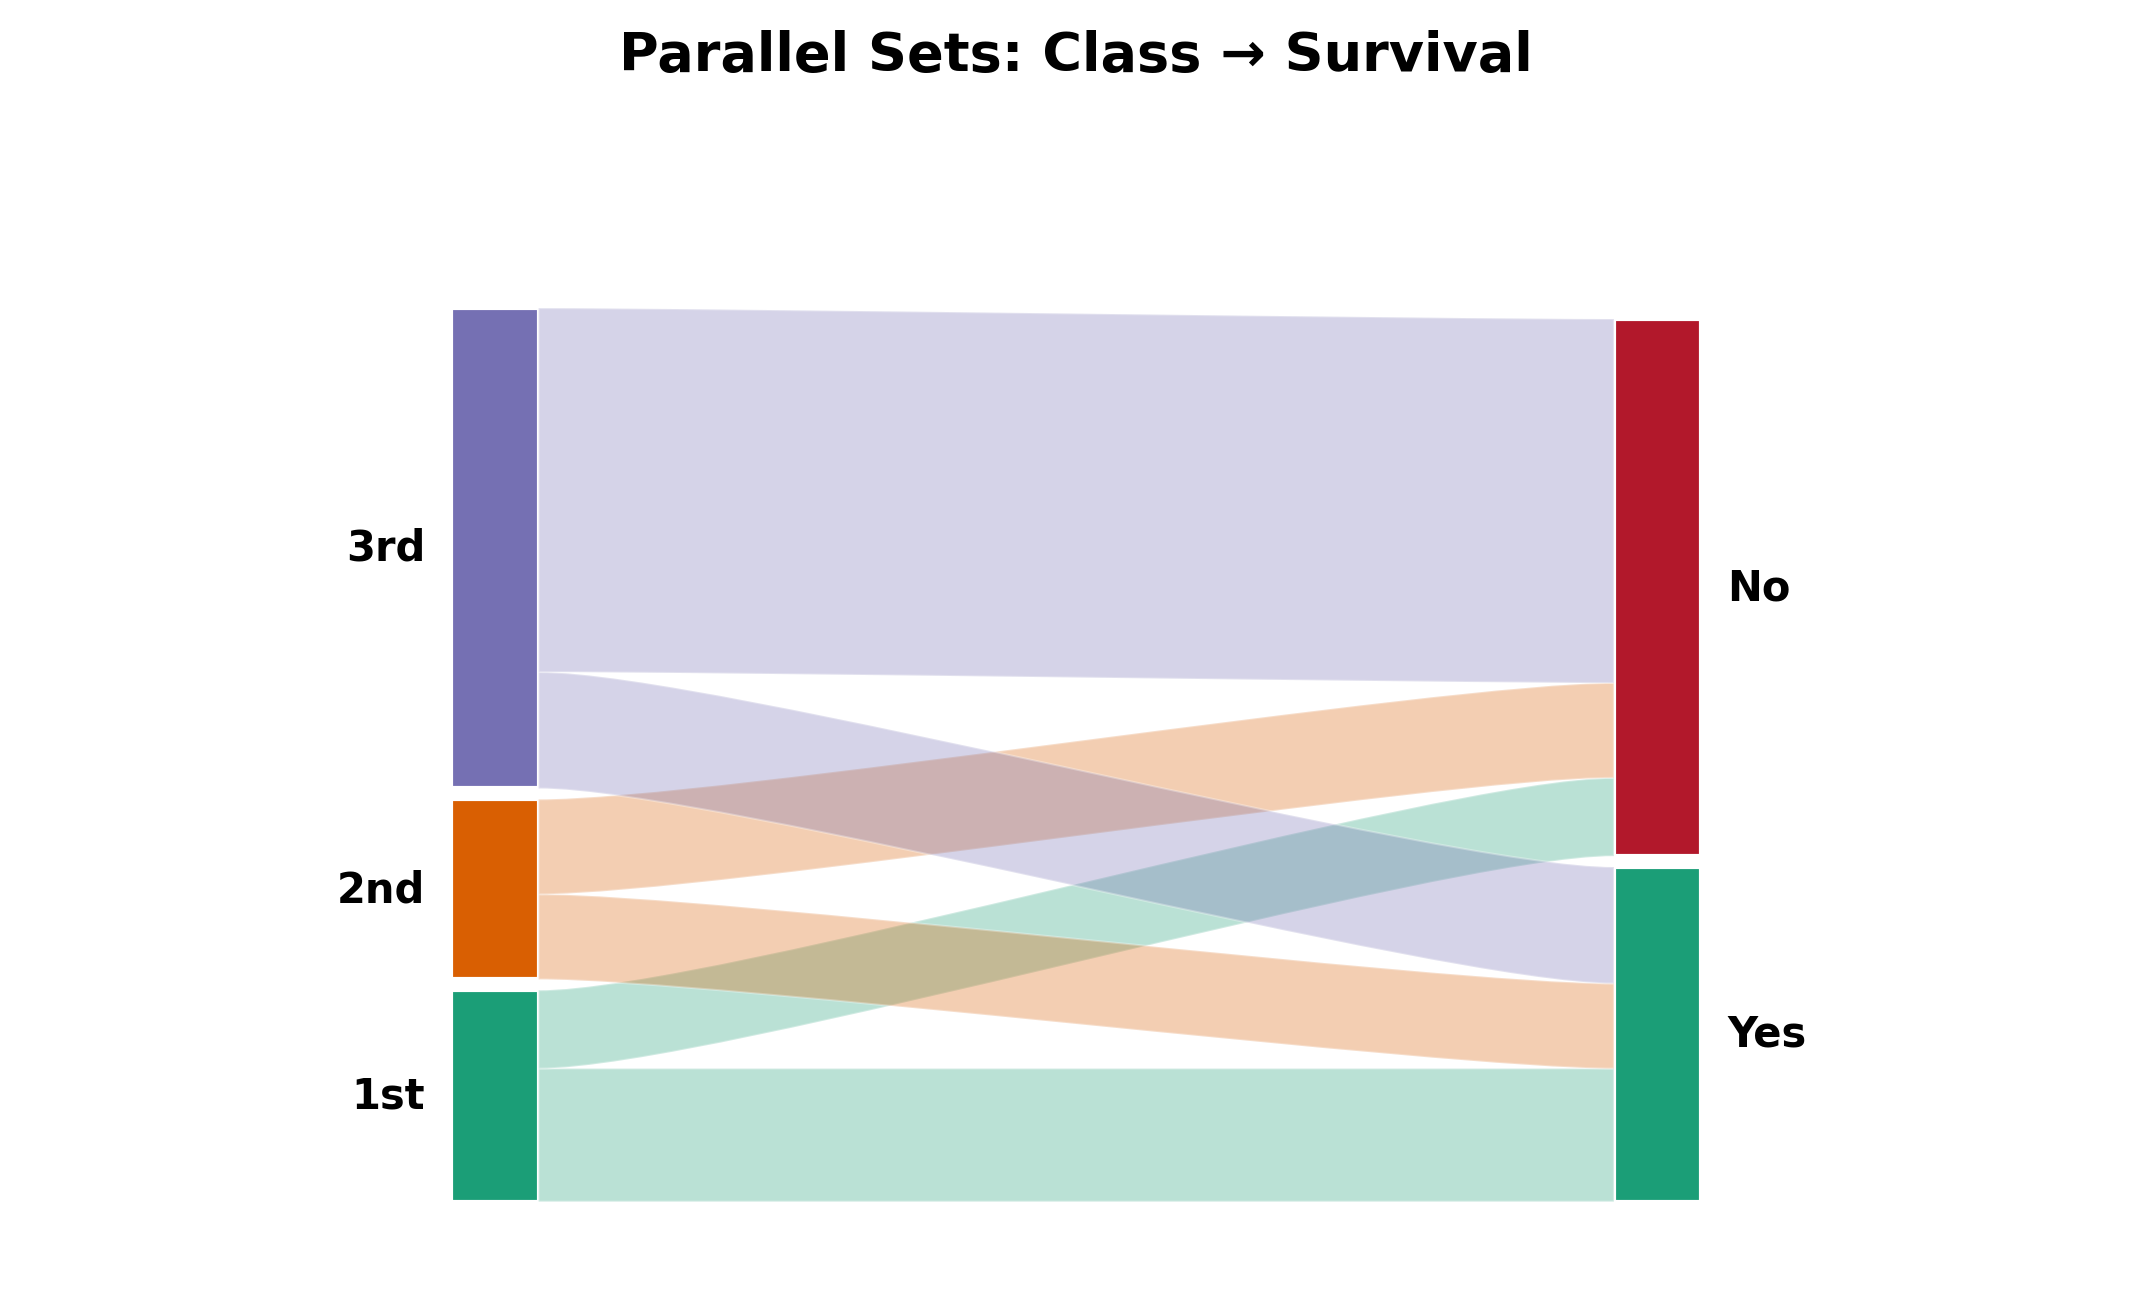
\includegraphics[width=0.68\textwidth]{m3_3_parallel_sets.png}

\vspace{0.2cm}
\begin{columns}[T]
\begin{column}{0.48\textwidth}
\begin{itemize}
    \item The categorical version of parallel coordinates
    \item Each axis = one categorical variable
    \item Ribbons connect categories across axes
    \item Width $\propto$ frequency of the combination
    \item Simpler than alluvial when only 2 variables
\end{itemize}
\end{column}
\begin{column}{0.48\textwidth}
\begin{alertblock}{Pro-Tip}
    \scriptsize R: \texttt{ggforce::geom\_parallel\_sets()} for ggplot2 integration. Python: \texttt{plotly.express.parallel\_categories()} for interactive display. Both handle 3+ axes gracefully.
\end{alertblock}
\end{column}
\end{columns}
\end{frame}

% ── 70 ──
\begin{frame}[fragile]{Parallel Sets --- Code}\smark{70/300}
\begin{columns}[T]
\begin{column}{0.48\textwidth}
\begin{lstlisting}[style=Rstyle]
library(ggforce)

# Prepare data
df_ps <- titanic |>
  gather_set_data(
    x = c("class","survived"))

ggplot(df_ps,
  aes(x, id = id,
      split = y, value = 1)) +
  geom_parallel_sets(
    aes(fill = class),
    alpha = 0.4) +
  geom_parallel_sets_axes(
    axis.width = 0.15) +
  geom_parallel_sets_labels(
    angle = 0, size = 3) +
  theme_void()
\end{lstlisting}
\end{column}
\begin{column}{0.48\textwidth}
\begin{lstlisting}[style=Pystyle]
import plotly.express as px

fig = px.parallel_categories(
    titanic,
    dimensions=["class","survived",
                "sex"],
    color="survived",
    color_continuous_scale=
        px.colors.qualitative.Set2)
fig.show()

# Static matplotlib: manual
# ribbon drawing (as in plots)
\end{lstlisting}
\vspace{0.1cm}
\begin{exampleblock}{Data Insight}
    \scriptsize \texttt{plotly.express.parallel\_categories()} is the easiest Python path --- interactive, with hover, reorderable axes. For static figures, the manual approach gives full control.
\end{exampleblock}
\end{column}
\end{columns}
\end{frame}

% ── 71 ──
\begin{frame}{Bump Charts: Rank Changes Over Time}
\smark{71/300}
\centering
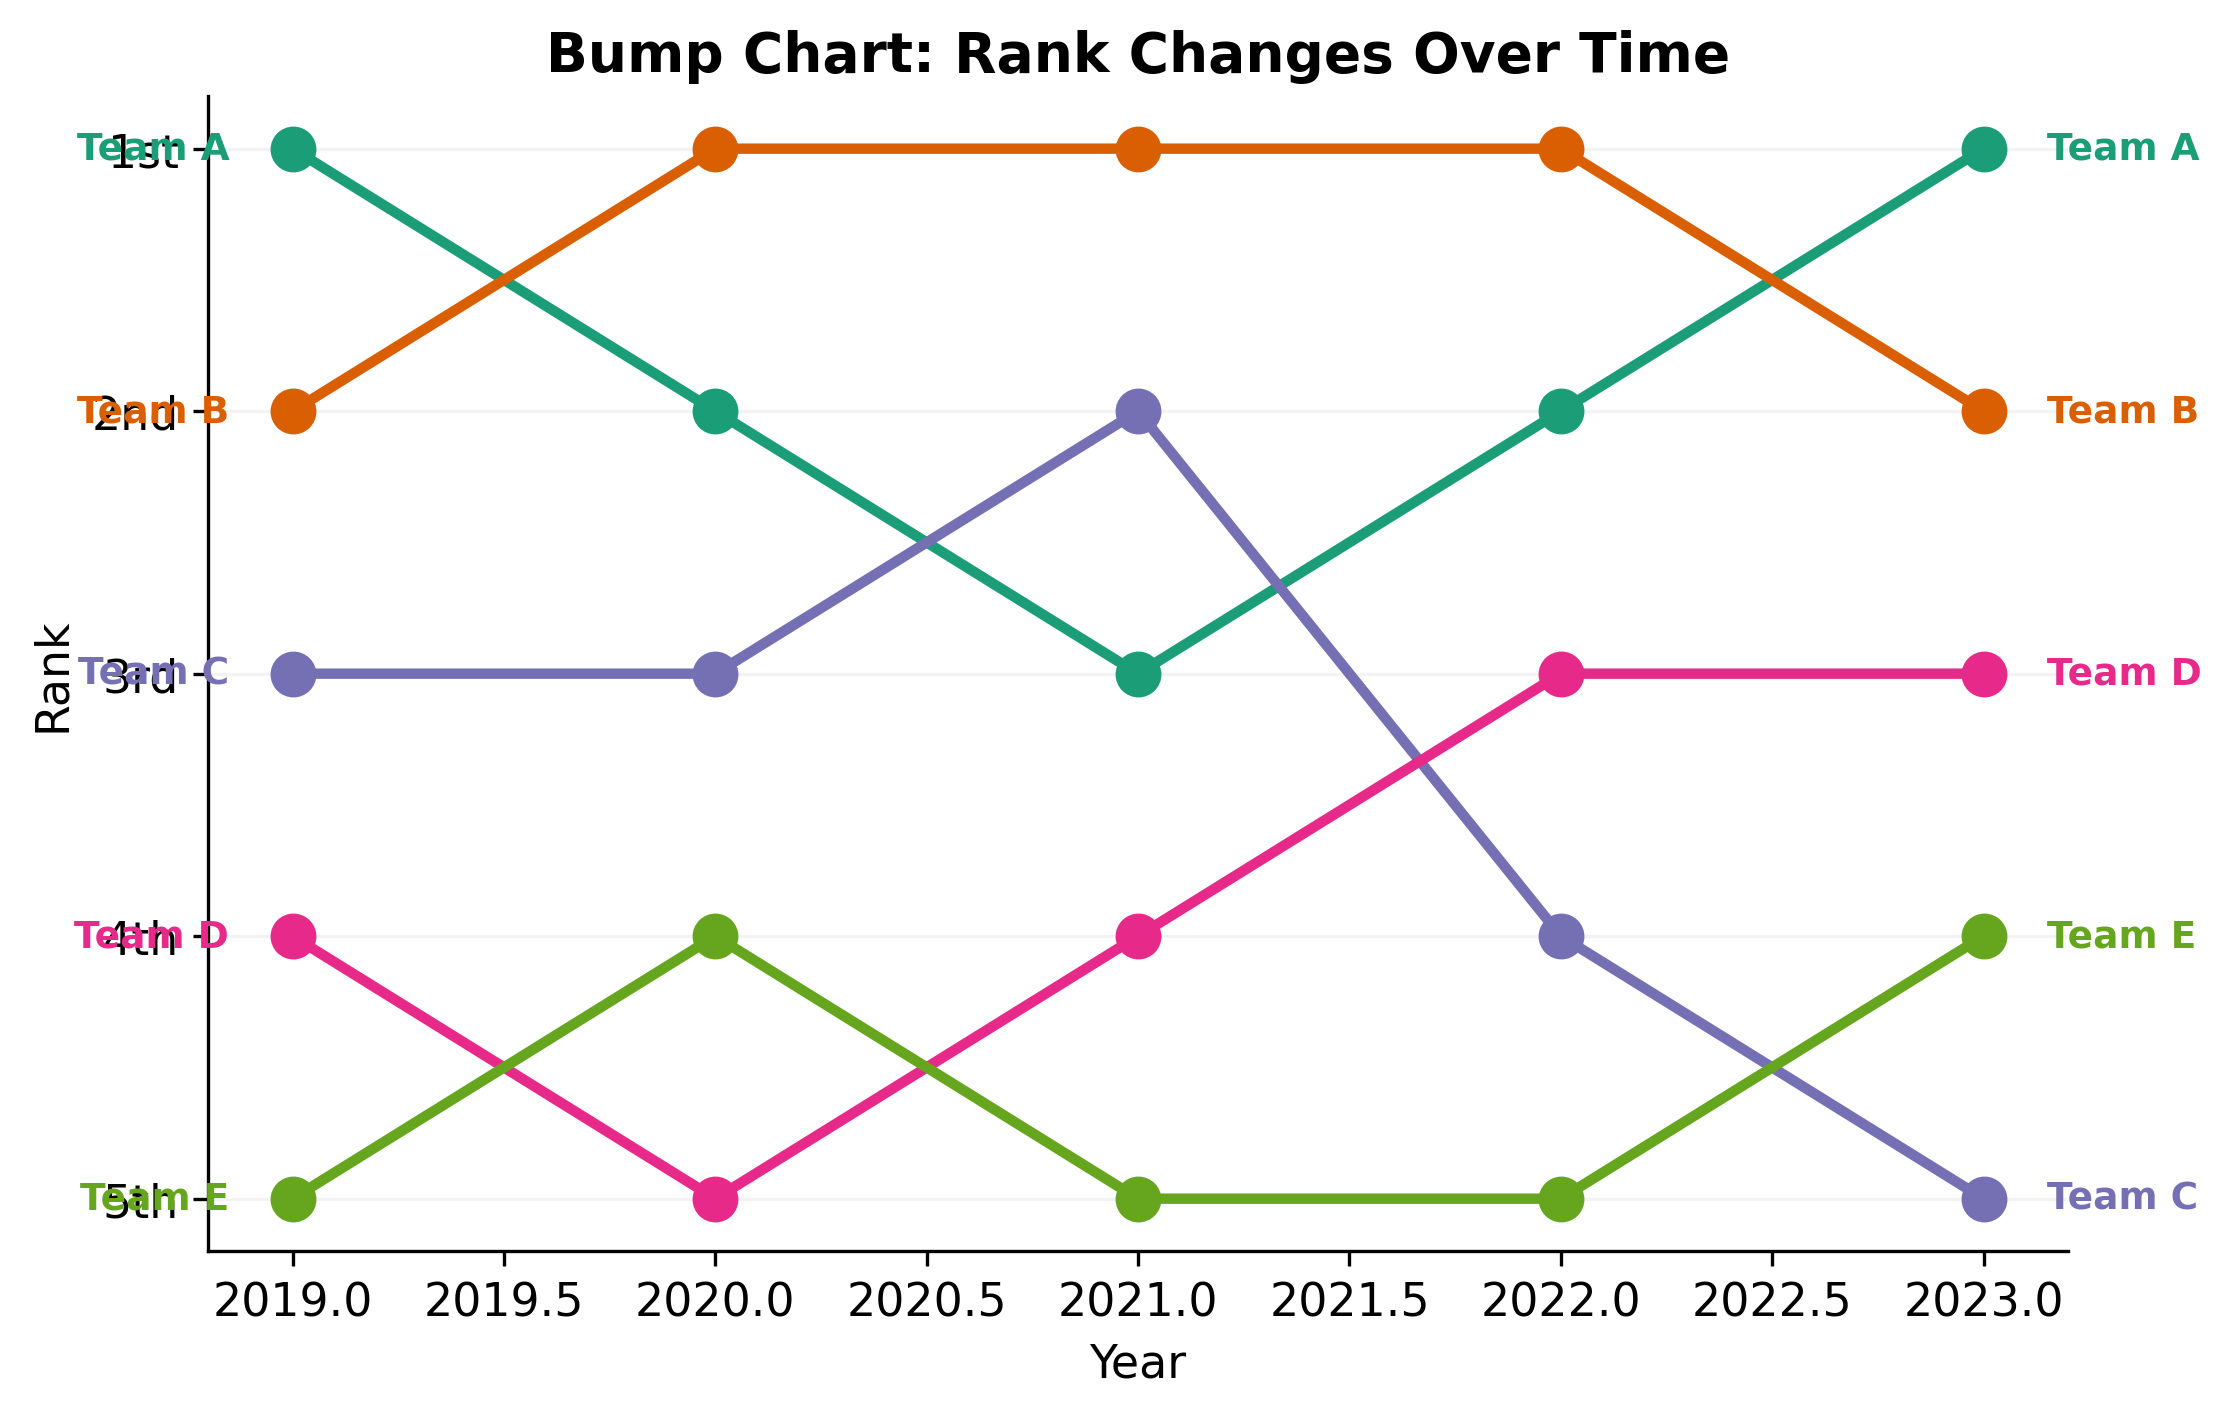
\includegraphics[width=0.72\textwidth]{m3_3_bump.png}

\vspace{0.2cm}
\begin{columns}[T]
\begin{column}{0.48\textwidth}
\begin{itemize}
    \item $x$-axis = time periods
    \item $y$-axis = rank (1 at top, inverted)
    \item Lines connect ranks across periods
    \item Crossings = rank changes
    \item Used for sports standings, brand rankings, election tracking
\end{itemize}
\end{column}
\begin{column}{0.48\textwidth}
\begin{exampleblock}{Data Insight}
    \scriptsize Team B held 1st place for three years before Team A reclaimed it. Team C collapsed from 3rd to 5th. The bump chart makes trajectories and crossover points immediately visible.
\end{exampleblock}
\end{column}
\end{columns}
\end{frame}

% ── 72 ──
\begin{frame}[fragile]{Bump Chart --- Code}\smark{72/300}
\begin{columns}[T]
\begin{column}{0.48\textwidth}
\begin{lstlisting}[style=Rstyle]
library(ggbump)

ggplot(ranking_df,
  aes(year, rank,
      color = team)) +
  geom_bump(linewidth = 1.5) +
  geom_point(size = 4) +
  geom_text(data = filter(
    ranking_df, year==max(year)),
    aes(label=team),
    hjust=-0.1, size=3) +
  scale_y_reverse() +
  theme_minimal()

# ggbump::geom_bump() adds smooth
# S-curve transitions between ranks
\end{lstlisting}
\end{column}
\begin{column}{0.48\textwidth}
\begin{lstlisting}[style=Pystyle]
fig, ax = plt.subplots()
for team, c in zip(teams, colors):
    r = ranks[team]
    ax.plot(years, r, "o-",
        color=c, linewidth=2.5,
        markersize=10)
    ax.text(years[-1]+0.15, r[-1],
        team, va="center",
        fontsize=9, color=c,
        fontweight="bold")
ax.invert_yaxis()
ax.set_yticks([1,2,3,4,5])
ax.set_yticklabels(
    ["1st","2nd","3rd","4th","5th"])
\end{lstlisting}
\vspace{0.1cm}
\begin{alertblock}{Pro-Tip}
    \scriptsize \texttt{ggbump} adds smooth S-curves instead of straight lines --- aesthetically superior. In matplotlib, use \texttt{scipy.interpolate} for smooth curves or just plot straight lines.
\end{alertblock}
\end{column}
\end{columns}
\end{frame}

% ── 73 ──
\begin{frame}{Slope Charts: Before/After Comparisons}
\smark{73/300}
\centering
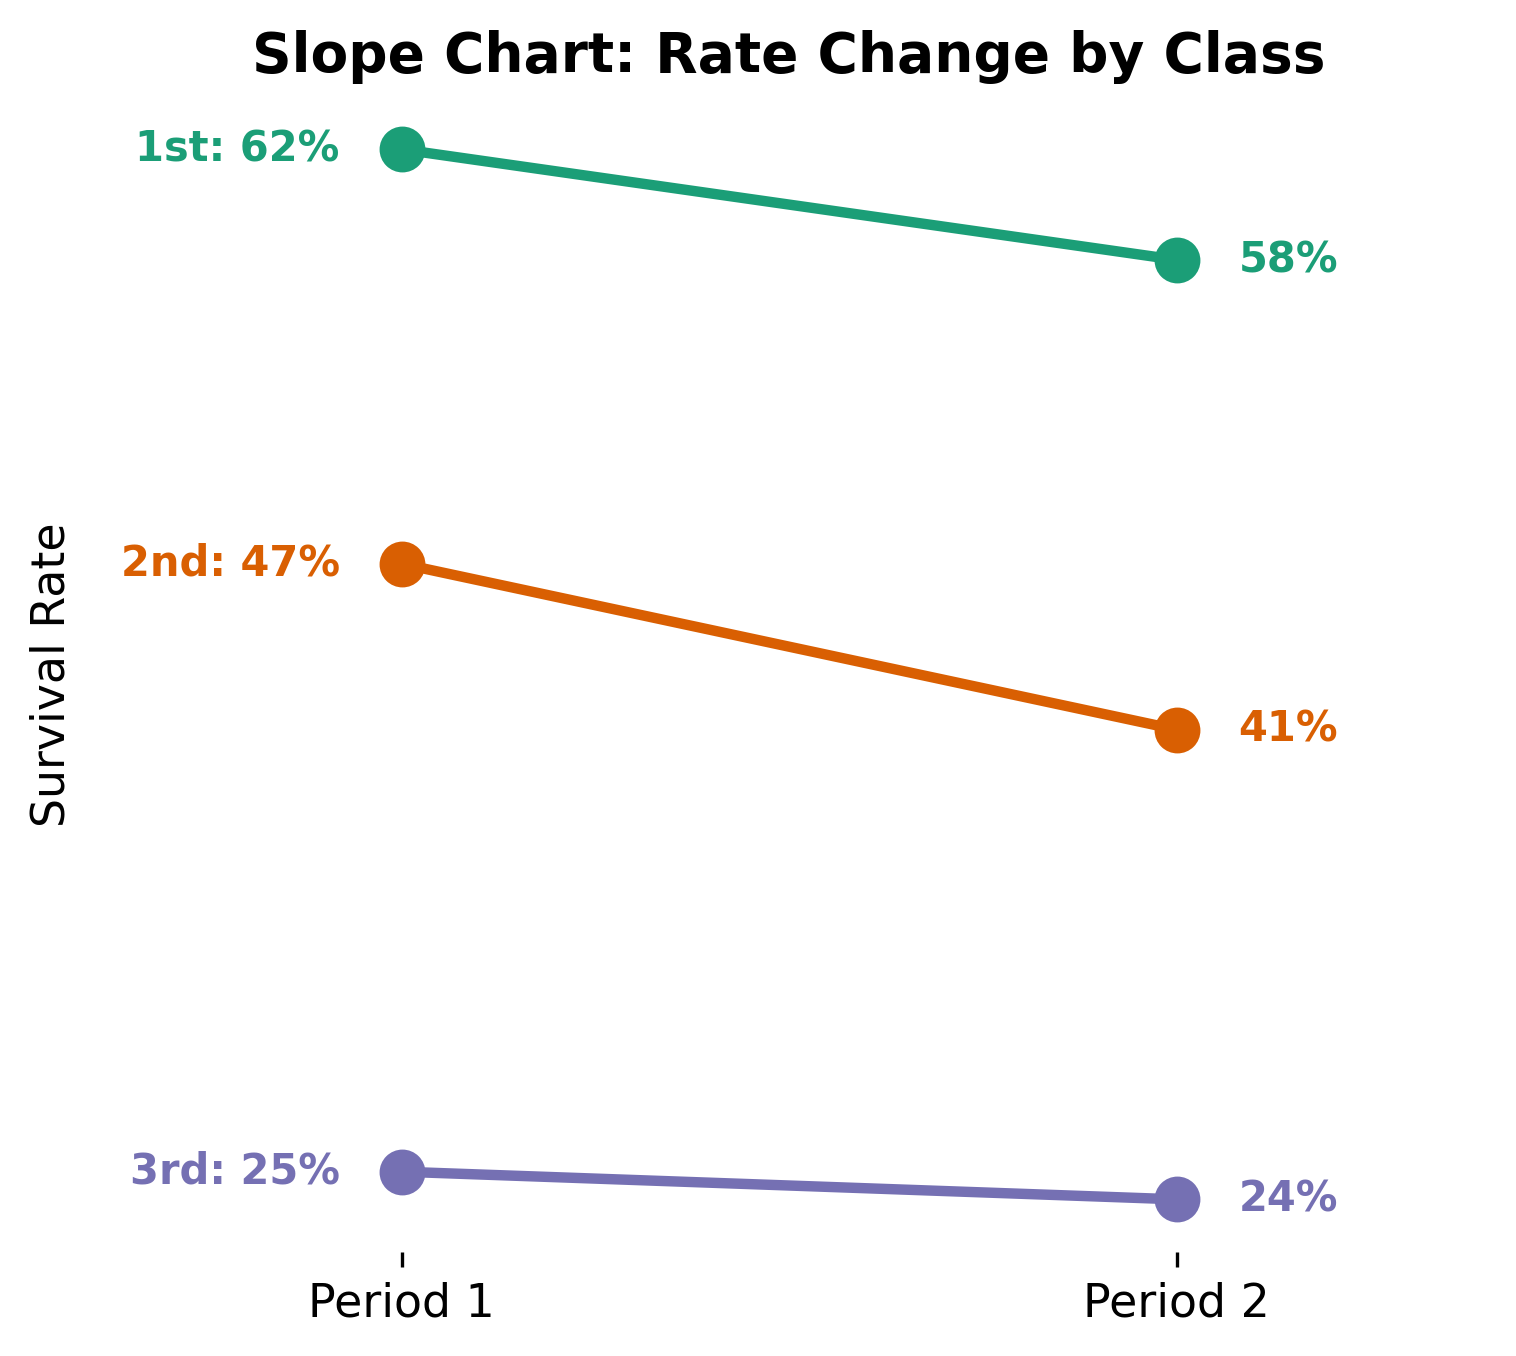
\includegraphics[width=0.55\textwidth]{m3_3_slope.png}

\vspace{0.2cm}
\begin{columns}[T]
\begin{column}{0.48\textwidth}
\begin{itemize}
    \item Two columns: before and after
    \item Lines connect the same entity across time
    \item Slope encodes direction and magnitude of change
    \item Direct labels at both ends eliminate the legend
    \item The ``minimal'' alternative to grouped bar charts
\end{itemize}
\end{column}
\begin{column}{0.48\textwidth}
\begin{exampleblock}{Data Insight}
    \scriptsize All classes declined slightly, but the rank order is preserved (no crossings). If lines crossed, it would indicate a rank reversal --- the most interesting pattern in a slope chart.
\end{exampleblock}
\vspace{0.1cm}
\begin{alertblock}{Pro-Tip}
    \scriptsize Slope charts work for 2--7 entities $\times$ 2 time points. For more entities, lines overlap. For more time points, use a bump chart or small-multiple line chart.
\end{alertblock}
\end{column}
\end{columns}
\end{frame}

% ── 74 ──
\begin{frame}[fragile]{Slope Chart --- Code}\smark{74/300}
\begin{columns}[T]
\begin{column}{0.48\textwidth}
\begin{lstlisting}[style=Rstyle]
# Manual in ggplot2
ggplot(df, aes(x=period, y=rate,
    group=class, color=class)) +
  geom_line(linewidth=1.5) +
  geom_point(size=4) +
  geom_text(data=filter(df,
    period=="Before"),
    aes(label=paste(class,
      scales::percent(rate))),
    hjust=1.1, size=3) +
  geom_text(data=filter(df,
    period=="After"),
    aes(label=scales::percent(rate)),
    hjust=-0.1, size=3) +
  theme_void()

# newggslopegraph() from CGPfunctions
library(CGPfunctions)
newggslopegraph(df, period,
  rate, class)
\end{lstlisting}
\end{column}
\begin{column}{0.48\textwidth}
\begin{lstlisting}[style=Pystyle]
fig, ax = plt.subplots()
for i, (cat, b, a) in enumerate(
    zip(categories, before, after)):
    ax.plot([0, 1], [b, a], "o-",
        color=colors[i], linewidth=2.5,
        markersize=10)
    ax.text(-0.08, b,
        f"{cat}: {b:.0%}",
        ha="right", fontweight="bold",
        color=colors[i])
    ax.text(1.08, a,
        f"{a:.0%}", ha="left",
        fontweight="bold",
        color=colors[i])
ax.set_xticks([0, 1])
ax.set_xticklabels(
    ["Period 1", "Period 2"])
ax.set_yticks([])
\end{lstlisting}
\end{column}
\end{columns}
\end{frame}

% ── 75 ──
\begin{frame}{UpSet Plots: Set Intersections Beyond Venn}
\smark{75/300}
\centering
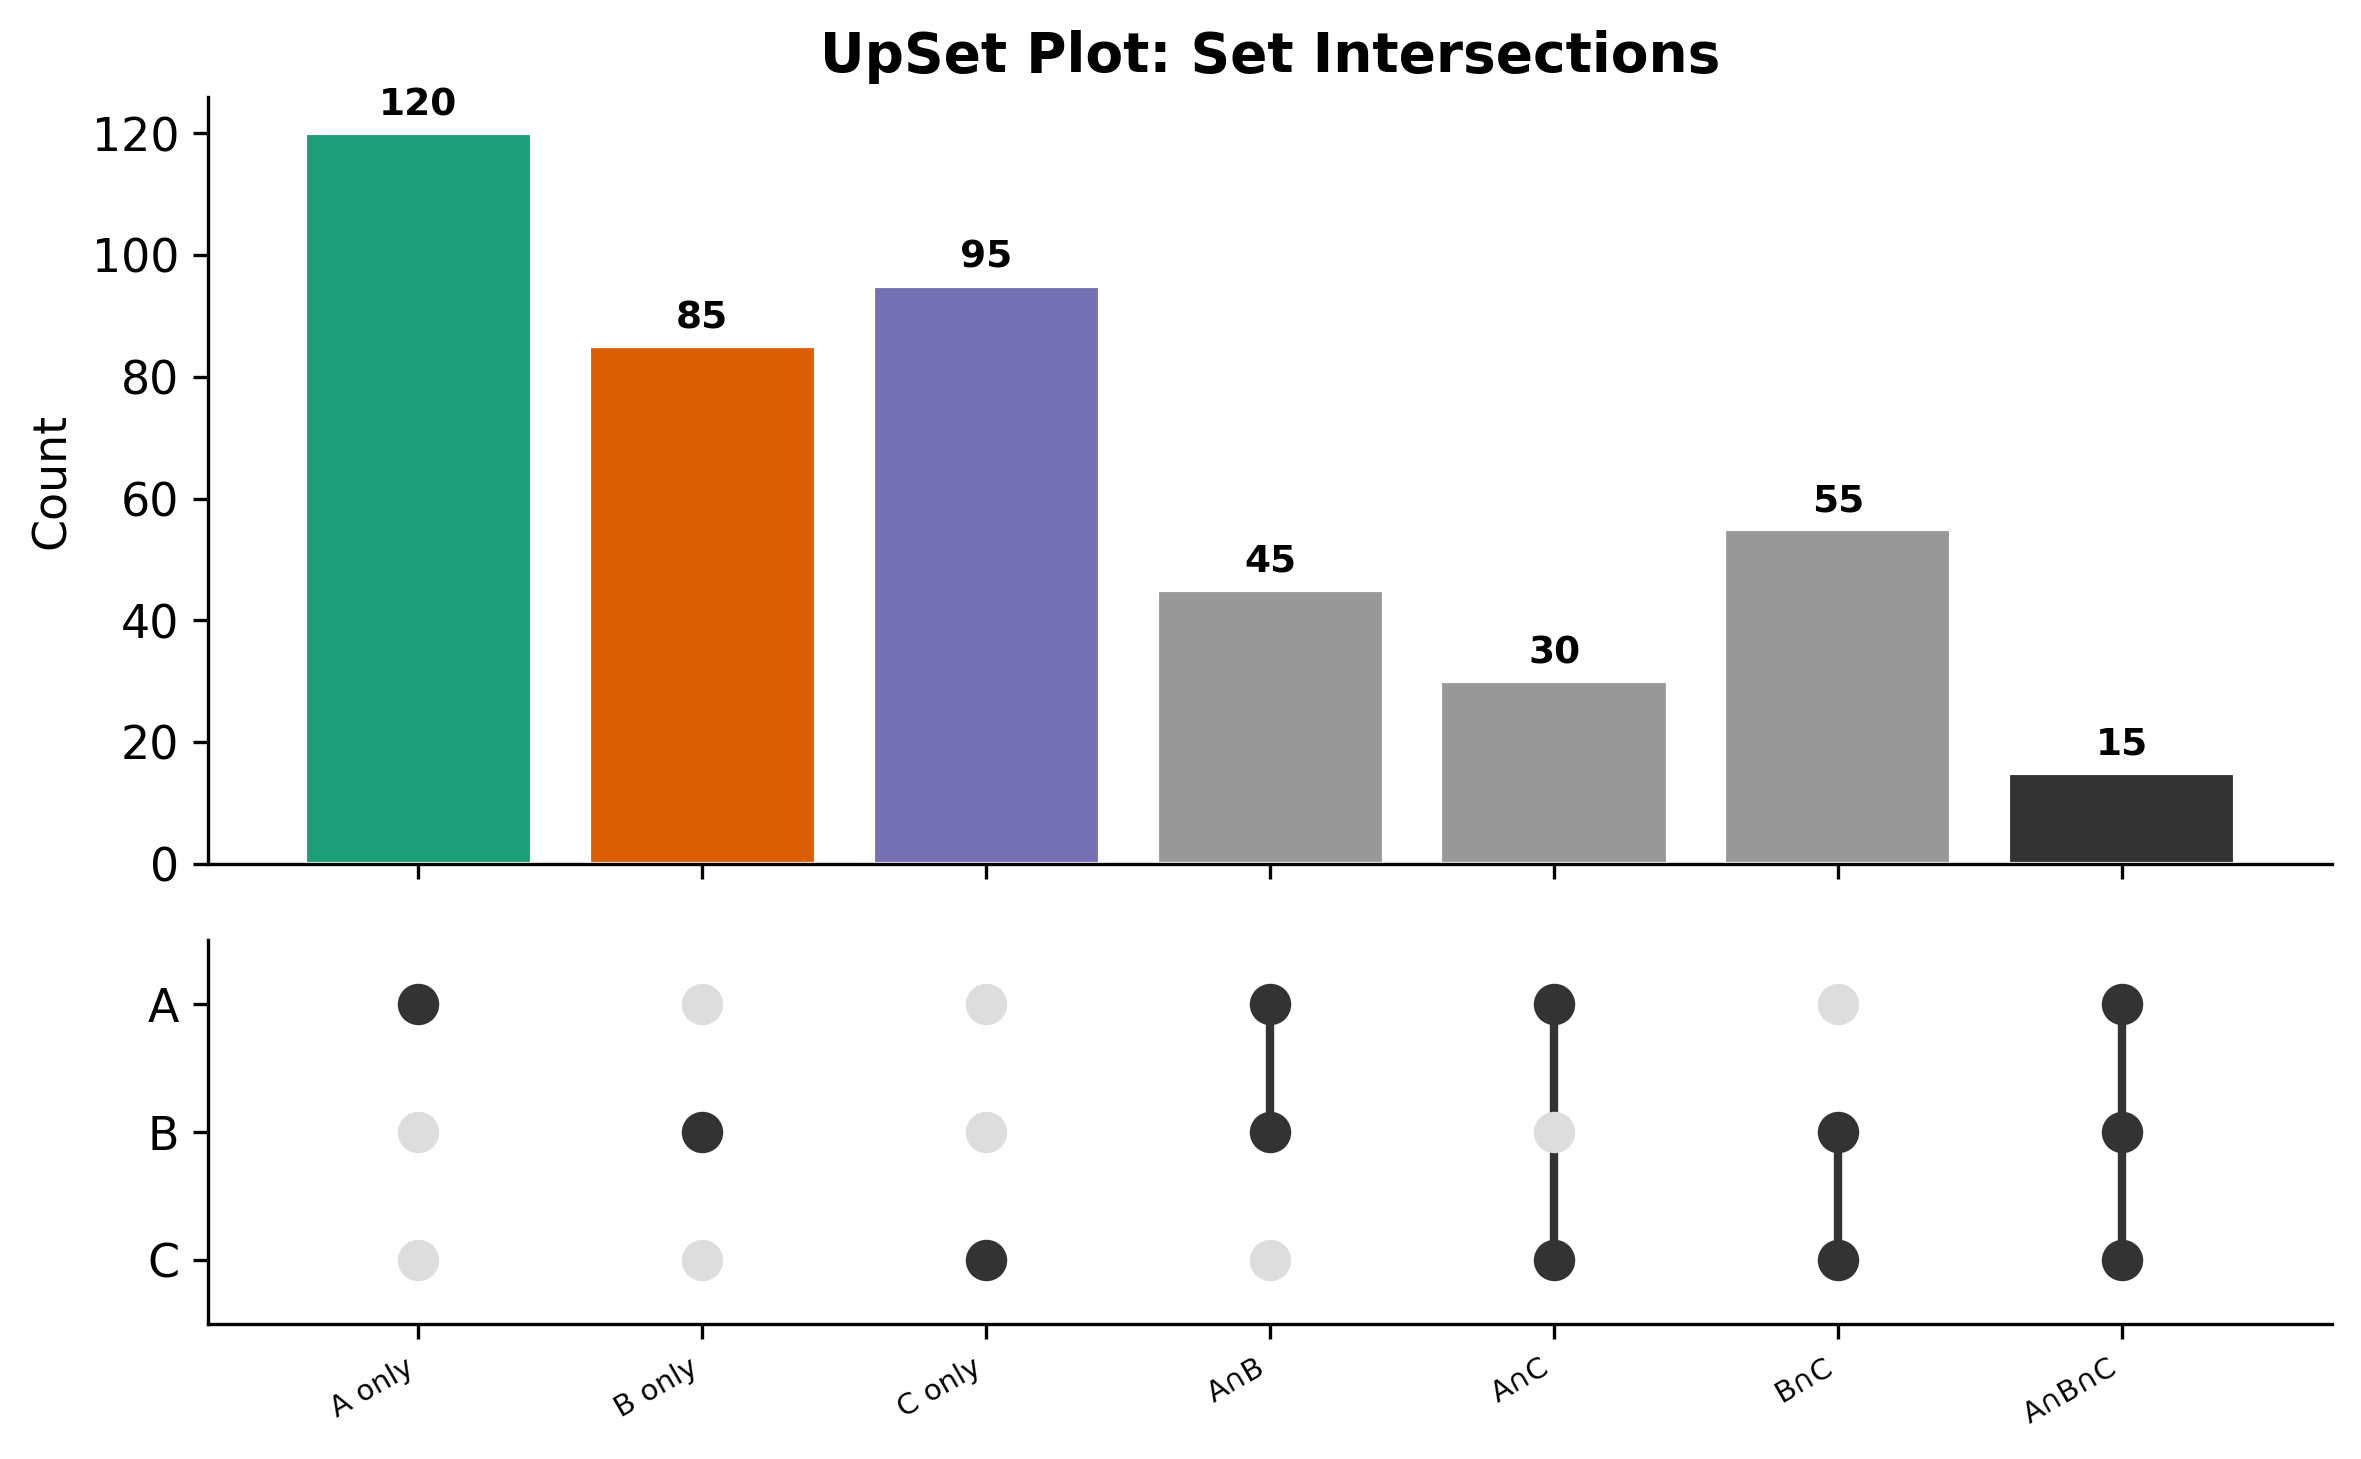
\includegraphics[width=0.72\textwidth]{m3_3_upset.png}

\vspace{0.2cm}
\begin{columns}[T]
\begin{column}{0.48\textwidth}
\begin{itemize}
    \item Replaces Venn diagrams for 3+ sets
    \item Top: bar chart of intersection sizes (sorted by count)
    \item Bottom: dot matrix showing which sets participate
    \item Connected dots = intersection of those sets
    \item Scales to 10+ sets (Venn fails at 4)
\end{itemize}
\end{column}
\begin{column}{0.48\textwidth}
\begin{exampleblock}{Data Insight}
    \scriptsize ``A only'' is the largest group (120). The triple intersection $A \cap B \cap C$ has only 15 members. UpSet plots rank intersections by size, making the most important ones immediately visible --- something Venn diagrams cannot do at scale.
\end{exampleblock}
\end{column}
\end{columns}
\end{frame}

% ── 76 ──
\begin{frame}[fragile]{UpSet Plot --- Code}\smark{76/300}
\begin{columns}[T]
\begin{column}{0.48\textwidth}
\begin{lstlisting}[style=Rstyle]
library(UpSetR)

# Input: binary membership matrix
upset(data,
  sets = c("A","B","C"),
  order.by = "freq",
  main.bar.color = "#2166AC",
  sets.bar.color = "#333",
  mb.ratio = c(0.6, 0.4))

# ComplexUpset (ggplot2-based)
library(ComplexUpset)
upset(data,
  intersect = c("A","B","C"),
  sort_intersections_by = "cardinality")
\end{lstlisting}
\end{column}
\begin{column}{0.48\textwidth}
\begin{lstlisting}[style=Pystyle]
# pip install upsetplot
from upsetplot import UpSet

# Input: MultiIndex Series
# with boolean membership
from upsetplot import from_memberships
data = from_memberships(
    [["A"], ["B"], ["A","B"],
     ["A","B","C"], ...],
    data=counts)

upset = UpSet(data,
    sort_by="cardinality",
    show_counts=True)
upset.plot()
\end{lstlisting}
\vspace{0.1cm}
\begin{alertblock}{Pro-Tip}
    \scriptsize \texttt{UpSetR} (R) and \texttt{upsetplot} (Python) are the dedicated packages. \texttt{ComplexUpset} (R) integrates with ggplot2 for custom annotations and faceting within the UpSet layout.
\end{alertblock}
\end{column}
\end{columns}
\end{frame}

% ── 77 ──
\begin{frame}{Venn Diagrams: Limited but Familiar}
\smark{77/300}
\begin{columns}[T]
\begin{column}{0.50\textwidth}
\begin{itemize}
    \item 2 sets: clear and effective
    \item 3 sets: acceptable but crowded
    \item 4+ sets: \textbf{impossible to draw accurately}
    \item Area is not proportional to count (common error)
    \item Use \textbf{proportional} Venn (Euler diagrams) for accuracy
\end{itemize}
\end{column}
\begin{column}{0.47\textwidth}
\begin{alertblock}{Pro-Tip}
    \scriptsize R: \texttt{ggVennDiagram} or \texttt{eulerr::euler()} for area-proportional diagrams. Python: \texttt{matplotlib-venn} for 2--3 sets, \texttt{upsetplot} for 4+. Always prefer UpSet over Venn for 3+ sets.
\end{alertblock}
\vspace{0.1cm}
\begin{exampleblock}{Data Insight}
    \scriptsize Euler diagrams differ from Venn: Euler only draws regions that have members. A 3-set Euler may omit the triple intersection if it's empty. This is more honest than showing an empty region.
\end{exampleblock}
\end{column}
\end{columns}
\end{frame}

% ── 78 ──
\begin{frame}[fragile]{Venn / Euler --- Code}\smark{78/300}
\begin{columns}[T]
\begin{column}{0.48\textwidth}
\begin{lstlisting}[style=Rstyle]
# Area-proportional Euler
library(eulerr)
fit <- euler(c(
  A=120, B=85, C=95,
  "A&B"=45, "A&C"=30,
  "B&C"=55, "A&B&C"=15))
plot(fit, fills=c("#1B9E77",
  "#D95F02","#7570B3"),
  alpha=0.4, quantities=TRUE)

# ggVennDiagram
library(ggVennDiagram)
ggVennDiagram(
  list(A=set_a, B=set_b, C=set_c),
  label_alpha=0) +
  scale_fill_gradient(
    low="white", high="#2166AC")
\end{lstlisting}
\end{column}
\begin{column}{0.48\textwidth}
\begin{lstlisting}[style=Pystyle]
from matplotlib_venn import (
    venn2, venn3)

# 2-set Venn
venn2(subsets=(120, 85, 45),
    set_labels=("A","B"))

# 3-set Venn
venn3(subsets=(120,85,45,95,30,55,15),
    set_labels=("A","B","C"))

# For 4+ sets: use UpSet
from upsetplot import UpSet
# (see previous slide)
\end{lstlisting}
\vspace{0.1cm}
\begin{exampleblock}{Data Insight}
    \scriptsize \texttt{matplotlib-venn} areas are \textbf{not} proportional by default. Use \texttt{eulerr} in R for true proportional diagrams.
\end{exampleblock}
\end{column}
\end{columns}
\end{frame}

% ── 79 ──
\begin{frame}{Patient Pathways and Funnel Flows}
\smark{79/300}
\begin{columns}[T]
\begin{column}{0.50\textwidth}
\begin{itemize}
    \item \textbf{Patient pathway}: diagnosis $\to$ treatment $\to$ outcome
    \item \textbf{Customer funnel}: visit $\to$ signup $\to$ purchase $\to$ retention
    \item \textbf{Dropout funnel}: each stage loses a fraction
    \item Alluvial/Sankey naturally show the narrowing
    \item Width at each stage = remaining cohort
\end{itemize}
\end{column}
\begin{column}{0.47\textwidth}
\begin{alertblock}{Pro-Tip}
    \scriptsize For funnel analysis, order stages left-to-right and make the progressive narrowing the visual focus. Annotate dropout percentages between stages. Color by dropout vs.\ retained.
\end{alertblock}
\vspace{0.1cm}
\begin{exampleblock}{Data Insight}
    \scriptsize E-commerce funnel: 10{,}000 visitors $\to$ 2{,}000 add-to-cart $\to$ 800 checkout $\to$ 600 purchase. The Sankey width shrinks at each stage, making the 94\% overall dropout visceral.
\end{exampleblock}
\end{column}
\end{columns}
\end{frame}

% ── 80 ──
\begin{frame}{When Flows Mislead: Design Principles}
\smark{80/300}
\centering\small
\begin{tabular}{@{}ll@{}}
    \toprule
    \textbf{Problem} & \textbf{Solution} \\
    \midrule
    Too many crossings (spaghetti)      & Reorder categories to minimize crossings \\
    Small flows invisible               & Filter: show only flows $> k$\% \\
    Color overload                      & Color by source OR destination, not both \\
    No annotation                       & Label flows with counts or percentages \\
    Implied directionality (left$\to$right) & Clarify if the relationship is not causal \\
    Area misperception                  & Width, not area, encodes magnitude \\
    Too many nodes                      & Aggregate small categories into ``Other'' \\
    \bottomrule
\end{tabular}

\vspace{0.3cm}
\begin{alertblock}{Pro-Tip}
    \scriptsize The single most common alluvial mistake: too many categories, producing an unreadable tangle. Collapse categories with $< 5$\% of total into ``Other'' before plotting. Readability trumps completeness.
\end{alertblock}
\end{frame}

% ── 81 ──
\begin{frame}{Alluvial Data Preparation}
\smark{81/300}
\begin{columns}[T]
\begin{column}{0.50\textwidth}
    \textbf{Wide format (one row per subject):}
    \begin{itemize}
        \item id, var1, var2, var3\ldots
        \item Each column = one axis
        \item \texttt{ggalluvial} requires this or lode form
    \end{itemize}
    \vspace{0.2cm}
    \textbf{Aggregated format (one row per combination):}
    \begin{itemize}
        \item var1, var2, var3, freq
        \item More compact for large datasets
        \item \texttt{plotly} Sankey uses node+link format
    \end{itemize}
\end{column}
\begin{column}{0.47\textwidth}
\begin{alertblock}{Pro-Tip}
    \scriptsize R: \texttt{ggalluvial::to\_lodes\_form()} converts wide $\to$ long. Python: \texttt{pd.crosstab()} or \texttt{groupby().size().reset\_index()} to aggregate. Plotly requires source/target/value link format.
\end{alertblock}
\vspace{0.1cm}
\begin{exampleblock}{Data Insight}
    \scriptsize For Plotly Sankey: nodes are integer-indexed. Source and target are arrays of node indices. Value is the flow magnitude. This format is unintuitive but flexible.
\end{exampleblock}
\end{column}
\end{columns}
\end{frame}

% ── 82 ──
\begin{frame}{Transition Matrices and Heatmaps}
\smark{82/300}
\begin{columns}[T]
\begin{column}{0.50\textwidth}
\begin{itemize}
    \item A transition matrix shows movement between states over time
    \item Row = state at $t$; column = state at $t+1$
    \item Cell value = count or probability of transition
    \item The ``flat'' alternative to an alluvial diagram
    \item Useful when you need exact numbers alongside the visual
\end{itemize}
\end{column}
\begin{column}{0.47\textwidth}
\begin{alertblock}{Pro-Tip}
    \scriptsize Visualize as a heatmap with \texttt{geom\_tile()} or \texttt{sns.heatmap()}. Annotate with transition probabilities. Row-normalize for transition probability matrix. This is the categorical analog of a confusion matrix.
\end{alertblock}
\vspace{0.1cm}
\begin{exampleblock}{Data Insight}
    \scriptsize Markov chain visualization: the transition matrix heatmap is the ``weights'' of the directed graph. The alluvial diagram is the ``flow'' through the graph. Both represent the same information.
\end{exampleblock}
\end{column}
\end{columns}
\end{frame}

% ── 83 ──
\begin{frame}[fragile]{Transition Matrix --- Code}\smark{83/300}
\begin{columns}[T]
\begin{column}{0.48\textwidth}
\begin{lstlisting}[style=Rstyle]
# Compute transition counts
trans <- table(df$state_t,
               df$state_t1)

# Transition probabilities
trans_prob <- prop.table(trans,
  margin = 1) # row-normalize

# Heatmap
library(reshape2)
ggplot(melt(trans_prob),
  aes(Var2, Var1, fill=value)) +
  geom_tile(color="white") +
  geom_text(aes(
    label=sprintf("%.0f%%",
      value*100)), size=3) +
  scale_fill_viridis_c() +
  labs(x="State t+1",
       y="State t") +
  coord_equal()
\end{lstlisting}
\end{column}
\begin{column}{0.48\textwidth}
\begin{lstlisting}[style=Pystyle]
# Compute
trans = pd.crosstab(
    df["state_t"], df["state_t1"])

# Row-normalize
trans_prob = trans.div(
    trans.sum(axis=1), axis=0)

# Heatmap
sns.heatmap(trans_prob,
    annot=True, fmt=".0%",
    cmap="viridis",
    linewidths=0.5, square=True)
plt.xlabel("State t+1")
plt.ylabel("State t")
\end{lstlisting}
\end{column}
\end{columns}
\end{frame}

% ── 84 ──
\begin{frame}{Flow Visualization Package Ecosystem}
\smark{84/300}
\centering\small
\begin{tabular}{@{}llll@{}}
    \toprule
    \textbf{Chart} & \textbf{R Package} & \textbf{Python} & \textbf{Interactive?} \\
    \midrule
    Alluvial        & \texttt{ggalluvial}         & \texttt{plotly}             & Yes (plotly) \\
    Sankey          & \texttt{networkD3}          & \texttt{plotly}             & Yes \\
    Parallel sets   & \texttt{ggforce}            & \texttt{plotly.express}     & Yes \\
    Bump chart      & \texttt{ggbump}             & Manual matplotlib           & No \\
    Slope chart     & \texttt{CGPfunctions}       & Manual matplotlib           & No \\
    UpSet plot      & \texttt{UpSetR}, \texttt{ComplexUpset} & \texttt{upsetplot} & No \\
    Venn / Euler    & \texttt{eulerr}             & \texttt{matplotlib-venn}    & No \\
    Funnel          & Manual / \texttt{ggsankey}  & \texttt{plotly.funnel}      & Yes \\
    \bottomrule
\end{tabular}
\end{frame}

% ── 85 ──
\begin{frame}{Flow Diagram Decision Guide}
\smark{85/300}
\centering\small
\begin{tabular}{@{}lll@{}}
    \toprule
    \textbf{Question} & \textbf{Chart} & \textbf{Key Feature} \\
    \midrule
    How do subjects partition across variables?  & Alluvial      & Same entities, multiple axes \\
    How does quantity flow between nodes?         & Sankey        & Conservation of flow \\
    How do categories co-occur across axes?       & Parallel sets & Categorical parallel coords \\
    How do ranks change over time?                & Bump chart    & Inverted y-axis, crossings \\
    How do values change between 2 periods?       & Slope chart   & Direct before/after \\
    Which set intersections are largest?           & UpSet plot    & Scales to 10+ sets \\
    How do subjects move between states?           & Transition heatmap & Exact probabilities \\
    Where does the cohort narrow?                  & Funnel / Sankey & Progressive dropout \\
    \bottomrule
\end{tabular}
\end{frame}

% ── 86 ──
\begin{frame}{Common Mistakes in Flow Diagrams}
\smark{86/300}
\centering\small
\begin{tabular}{@{}ll@{}}
    \toprule
    \textbf{Mistake} & \textbf{Fix} \\
    \midrule
    Too many categories (spaghetti)          & Aggregate small flows into ``Other'' \\
    Venn for 4+ sets                         & Switch to UpSet plot \\
    Non-proportional Venn areas              & Use \texttt{eulerr} for Euler diagrams \\
    Alluvial implying causation              & State explicitly if the flow is not causal \\
    Sankey with inconsistent totals          & Verify conservation: input = output per node \\
    No annotations on flows                  & Label top 3--5 flows with counts \\
    Bump chart with too many entities         & Show top 5--7; grey out the rest \\
    \bottomrule
\end{tabular}
\end{frame}

% ── 87 ──
\begin{frame}{Treemaps: Hierarchical Composition}
\smark{87/300}
\begin{columns}[T]
\begin{column}{0.50\textwidth}
\begin{itemize}
    \item Nested rectangles encoding hierarchical part-of-whole
    \item Area $\propto$ value (count, revenue, population)
    \item Color can encode a second variable
    \item Scales to hundreds of categories via nesting
    \item Useful for file systems, budgets, market cap
\end{itemize}
\end{column}
\begin{column}{0.47\textwidth}
\begin{alertblock}{Pro-Tip}
    \scriptsize R: \texttt{treemapify::geom\_treemap()} for ggplot2; \texttt{treemap::treemap()} for base. Python: \texttt{squarify.plot()} or \texttt{plotly.express.treemap()}. Interactive treemaps (plotly) allow drill-down into nested levels.
\end{alertblock}
\vspace{0.1cm}
\begin{exampleblock}{Data Insight}
    \scriptsize Treemaps encode area (rank 5, Cleveland). They are best for giving an \emph{overview} of hierarchical composition, not for precise comparison. For exact values, add labels or use a bar chart.
\end{exampleblock}
\end{column}
\end{columns}
\end{frame}

% ── 88 ──
\begin{frame}[fragile]{Treemap --- Code}\smark{88/300}
\begin{columns}[T]
\begin{column}{0.48\textwidth}
\begin{lstlisting}[style=Rstyle]
library(treemapify)

ggplot(budget_df,
  aes(area = amount,
      fill = department,
      label = paste(department,
        scales::dollar(amount)),
      subgroup = division)) +
  geom_treemap() +
  geom_treemap_text(
    place = "centre",
    size = 9, color = "white") +
  geom_treemap_subgroup_border(
    color = "white", size = 2) +
  theme(legend.position="none")
\end{lstlisting}
\end{column}
\begin{column}{0.48\textwidth}
\begin{lstlisting}[style=Pystyle]
import squarify

sizes = [500, 300, 200, 150, 100]
labels = ["R&D","Sales","Ops",
          "Marketing","Admin"]
colors = ["#1B9E77","#D95F02",
    "#7570B3","#E7298A","#66A61E"]

squarify.plot(sizes=sizes,
    label=labels, color=colors,
    alpha=0.7, text_kwargs={
        "fontsize":10,
        "fontweight":"bold"})
plt.axis("off")

# Interactive (plotly)
import plotly.express as px
fig = px.treemap(df,
    path=["division","department"],
    values="amount")
\end{lstlisting}
\end{column}
\end{columns}
\end{frame}

% ── 89 ──
\begin{frame}{Sunburst Charts: Radial Treemaps}
\smark{89/300}
\begin{columns}[T]
\begin{column}{0.50\textwidth}
\begin{itemize}
    \item Hierarchical composition in radial layout
    \item Inner ring = top level; outer rings = sub-categories
    \item Arc length $\propto$ value
    \item More compact than treemaps for deep hierarchies
    \item Best as interactive (click to zoom)
\end{itemize}
\end{column}
\begin{column}{0.47\textwidth}
\begin{alertblock}{Pro-Tip}
    \scriptsize R: \texttt{plotly::plot\_ly(type="sunburst")} or \texttt{sunburstR}. Python: \texttt{plotly.express.sunburst()}. Sunbursts use angle encoding (rank 4) --- less accurate than treemaps (area, rank 5) for comparison. Use for overview navigation, not precision.
\end{alertblock}
\end{column}
\end{columns}
\end{frame}

% ── 90 ──
\begin{frame}{Module 3.3 --- Key Takeaways}\smark{90/300}
\begin{enumerate}
    \item \textbf{Alluvial diagrams} show how subjects partition across categorical variables.
    \item \textbf{Sankey diagrams} show conserved quantity flows between nodes.
    \item \textbf{Bump charts} reveal rank changes over time; \textbf{slope charts} show before/after.
    \item \textbf{UpSet plots} replace Venn diagrams for 3+ sets.
    \item \textbf{Treemaps} handle hierarchical composition; \textbf{sunbursts} add radial layout.
    \item \textbf{Minimize crossings}, aggregate small flows, and always annotate top flows.
\end{enumerate}
\end{frame}

% ── 91 ──
\begin{frame}{}\smark{91/300}
\centering\vspace{1.5cm}
{\Large\textbf{Module 3.3 Complete}}\\[0.5cm]
You can now build alluvial, Sankey, parallel-set, bump, slope, UpSet, treemap, and sunburst charts --- and know when each flow diagram is appropriate.\\[0.5cm]
\textbf{Next:} Module 3.4 --- Likert Scales, Diverging Stacked Bars, and Survey Data.
\end{frame}

% ═══════════════════════════════════════════════════════
%  MODULE 3.4 — Likert Scales, Diverging Stacked Bars, and Survey Data
% ═══════════════════════════════════════════════════════
\section{Module 3.4 --- Likert Scales and Survey Data}

% ── 92 ──
\begin{frame}{Module 3.4 --- Roadmap}\smark{92/300}
\begin{enumerate}
    \item Likert scales: what they are and are not
    \item Standard vs.\ diverging stacked bars
    \item Centering at neutral: the diverging layout
    \item Net scores: Agree $-$ Disagree
    \item Likert heatmaps for multi-item batteries
    \item Mean scores alongside distributions
    \item Net Promoter Score (NPS) visualization
    \item Design principles for survey data
\end{enumerate}
\end{frame}

% ── 93 ──
\begin{frame}{Likert Scales: What They Are}
\smark{93/300}
\begin{columns}[T]
\begin{column}{0.50\textwidth}
\begin{itemize}
    \item Ordinal response scale (typically 5 or 7 points)
    \item Anchors: Strongly Disagree $\to$ Strongly Agree
    \item A \textbf{Likert item} = one question
    \item A \textbf{Likert scale} = a battery of items measuring one construct
    \item Strictly ordinal, but often treated as interval in practice
\end{itemize}
\end{column}
\begin{column}{0.47\textwidth}
\begin{alertblock}{Pro-Tip}
    \scriptsize The debate: can you compute means on Likert data? Purists say no (ordinal). Pragmatists say yes (with 5+ points, the approximation works). Visualization sidesteps the debate: show the \textbf{full distribution}, not just the mean.
\end{alertblock}
\vspace{0.1cm}
\begin{exampleblock}{Data Insight}
    \scriptsize 5-point: SD, D, N, A, SA. 7-point adds ``Slightly Disagree'' and ``Slightly Agree.'' More points $\to$ more discrimination but longer completion time.
\end{exampleblock}
\end{column}
\end{columns}
\end{frame}

% ── 94 ──
\begin{frame}{Standard vs.\ Diverging Stacked Bars}
\smark{94/300}
\centering
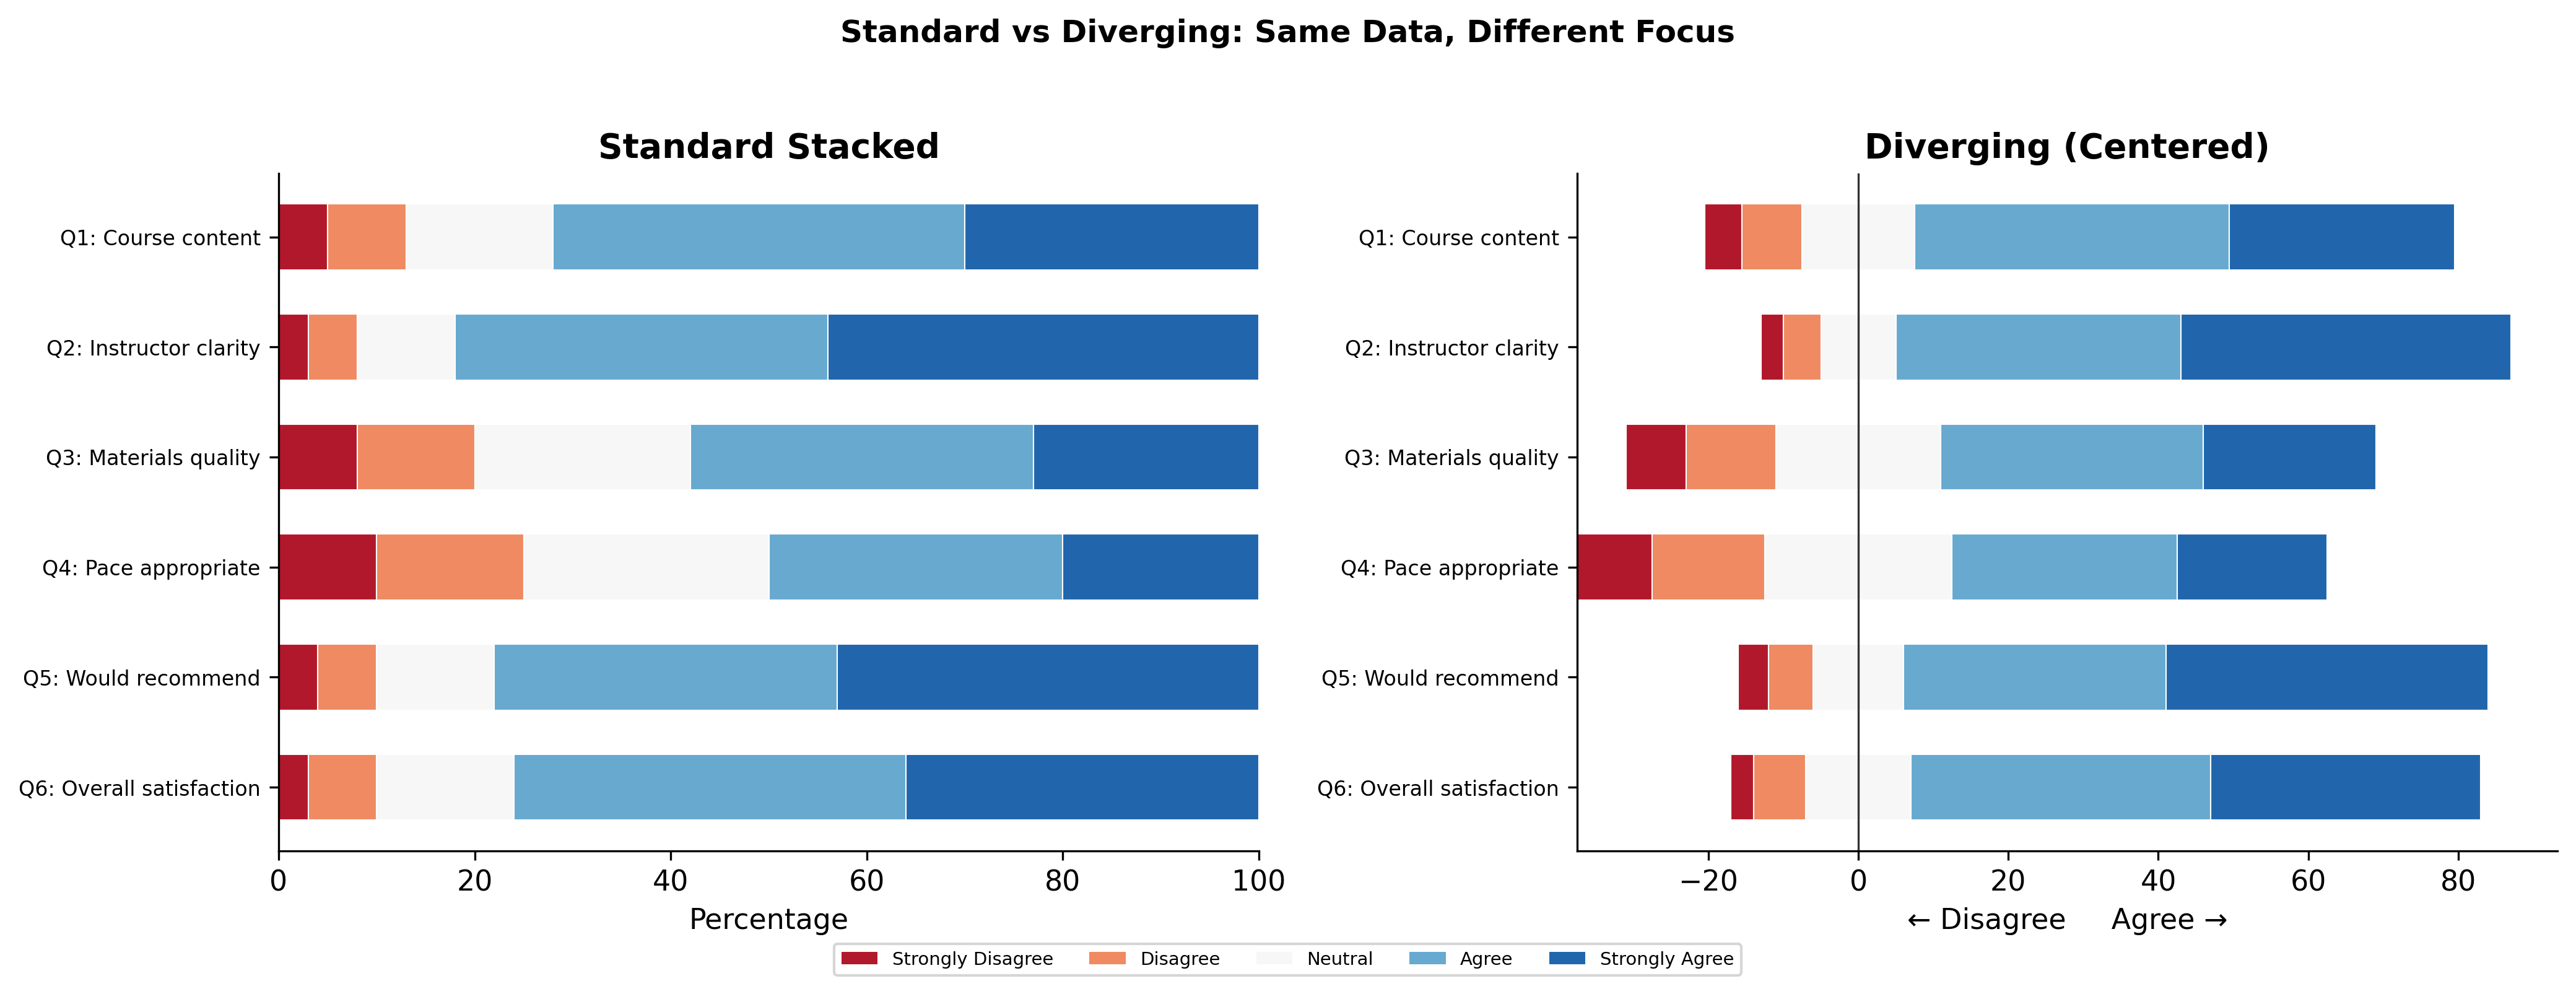
\includegraphics[width=0.92\textwidth]{m3_4_std_vs_div.png}

\vspace{0.2cm}
\begin{exampleblock}{Data Insight}
    \scriptsize Left (standard): all bars start at 0, good for reading individual segment sizes. Right (diverging): centered at neutral, good for comparing the \textbf{balance of agreement vs.\ disagreement} across questions. The diverging layout is the standard for Likert survey reports.
\end{exampleblock}
\end{frame}

% ── 95 ──
\begin{frame}{The Diverging Stacked Bar}
\smark{95/300}
\centering
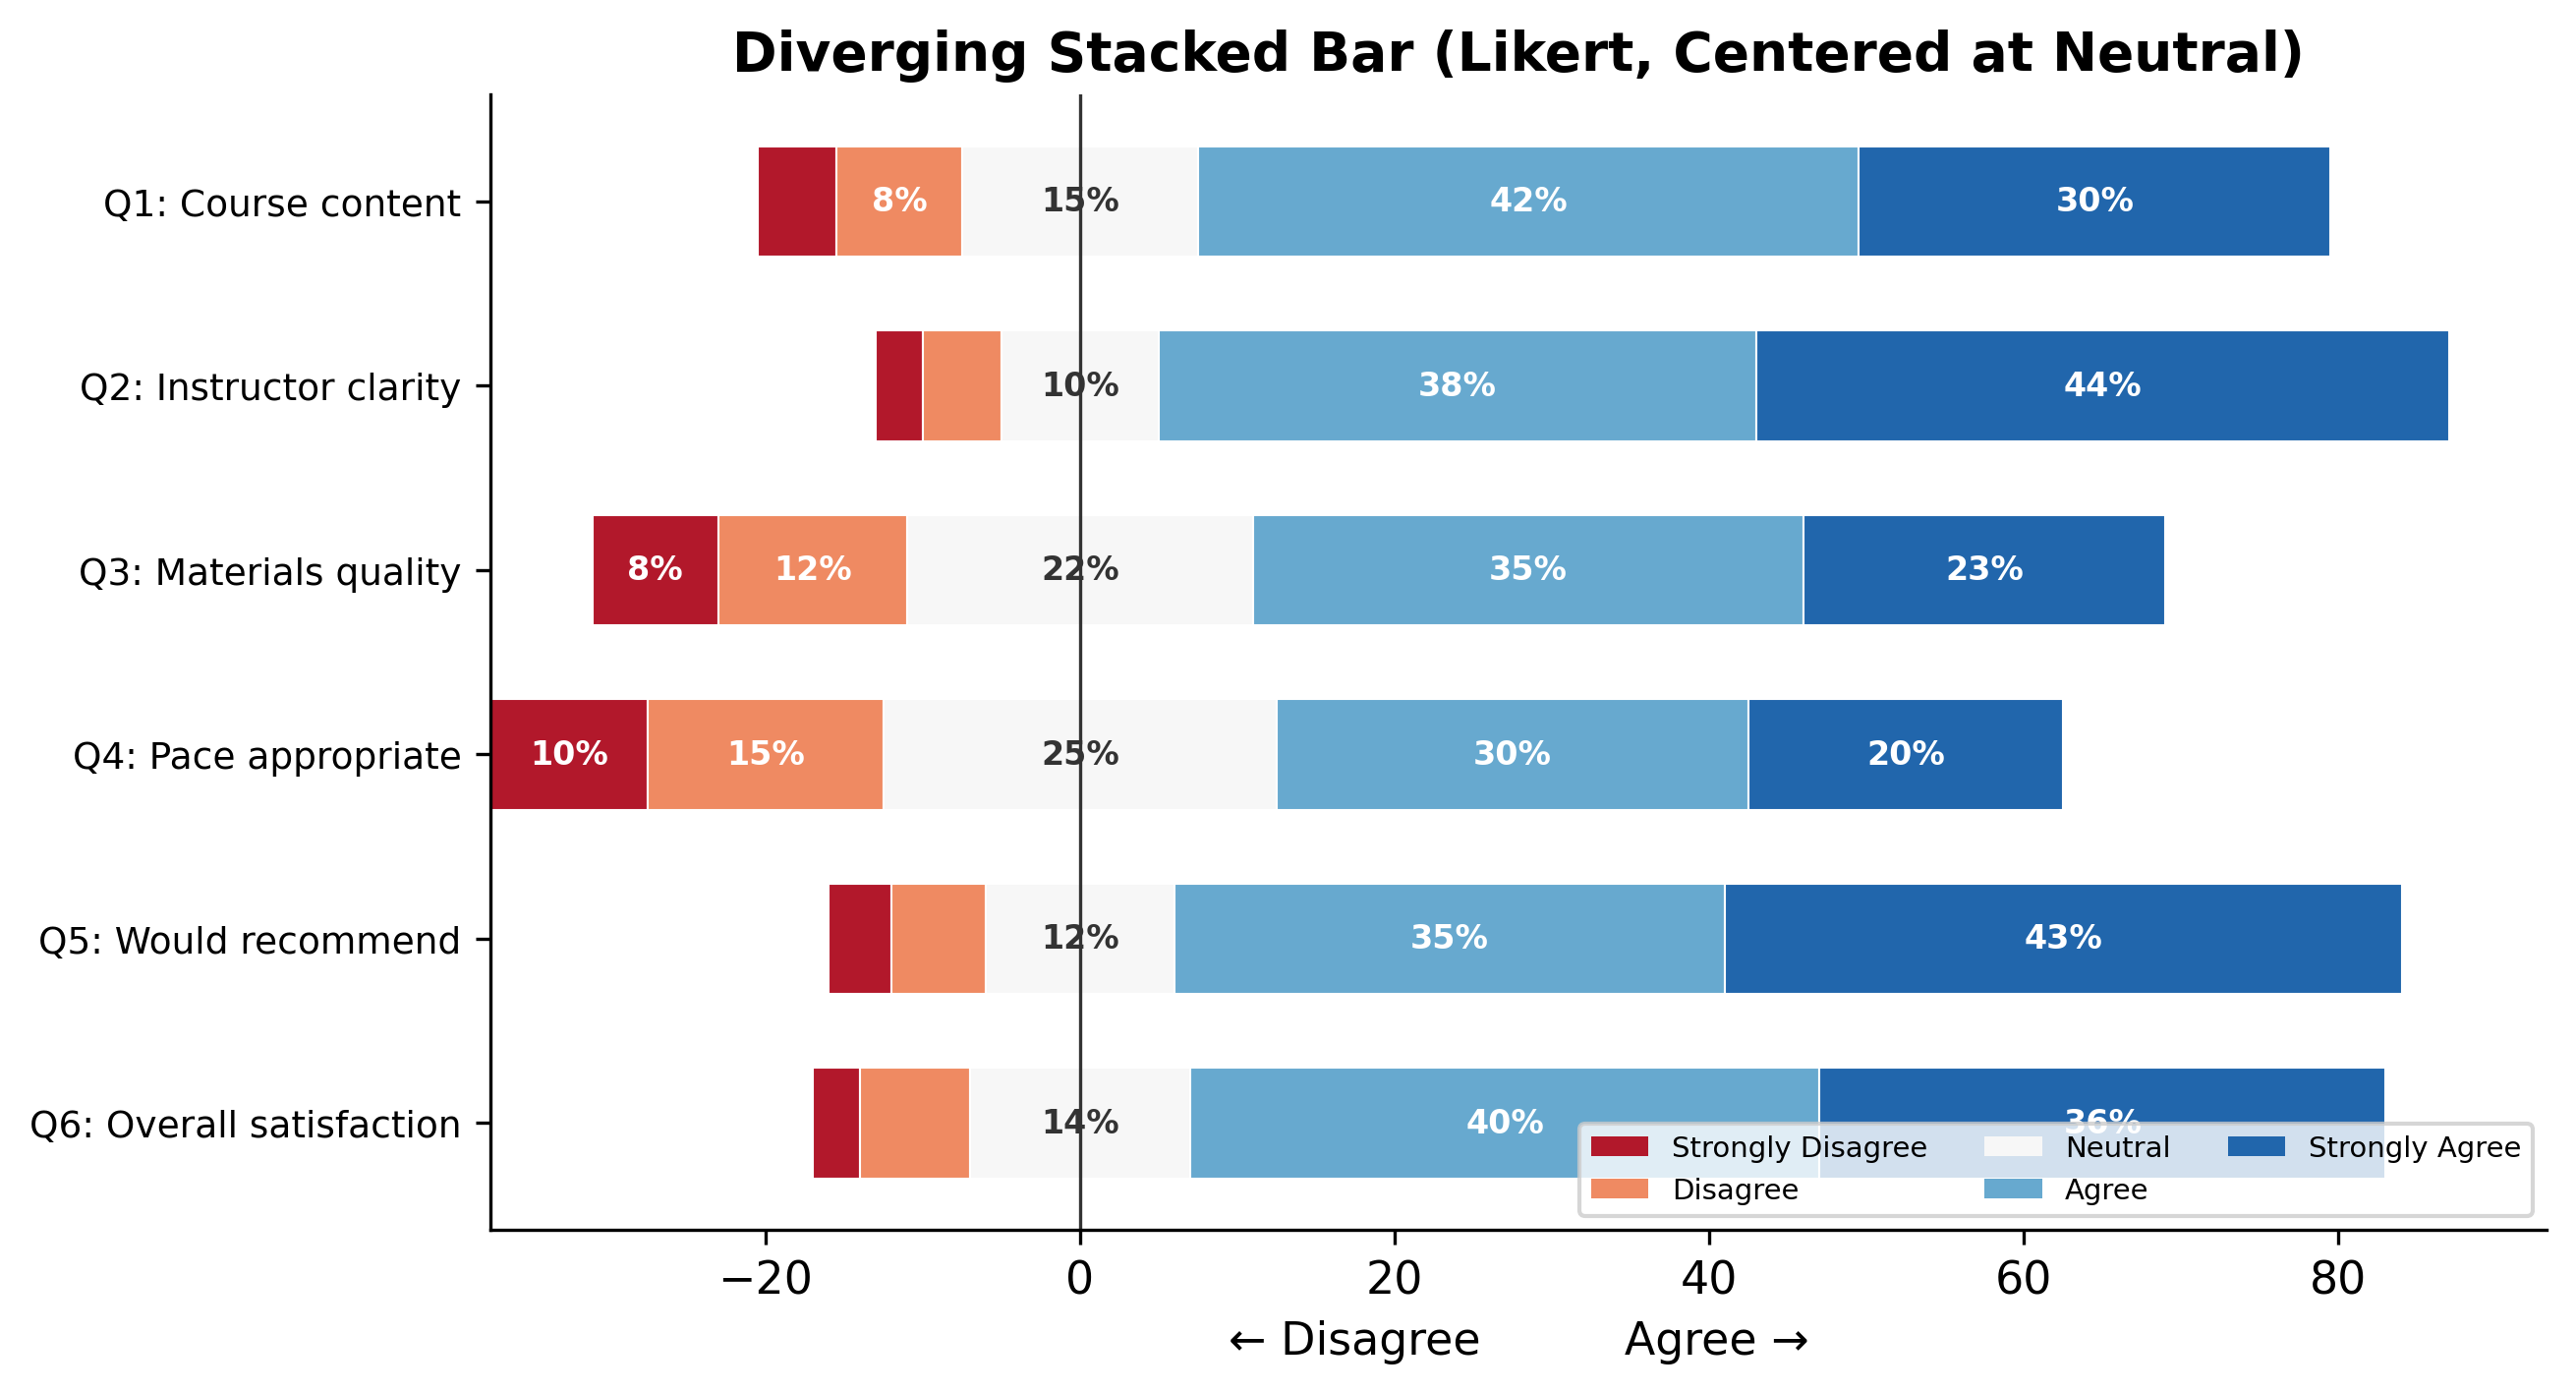
\includegraphics[width=0.78\textwidth]{m3_4_diverging_stacked.png}

\vspace{0.2cm}
\begin{columns}[T]
\begin{column}{0.48\textwidth}
\begin{itemize}
    \item Negative responses extend \textbf{left} of center
    \item Positive responses extend \textbf{right}
    \item Neutral is \textbf{split} half-left, half-right
    \item The center line is a visual ``zero point''
    \item Questions with more agreement extend further right
\end{itemize}
\end{column}
\begin{column}{0.48\textwidth}
\begin{alertblock}{Pro-Tip}
    \scriptsize Use a \textbf{diverging color palette}: red tones for disagree, blue tones for agree, grey/white for neutral. This matches the semantic content of the scale.
\end{alertblock}
\end{column}
\end{columns}
\end{frame}

% ── 96 ──
\begin{frame}[fragile]{Diverging Stacked Bar --- \Rlang}\smark{96/300}
\begin{columns}[T]
\begin{column}{0.55\textwidth}
\begin{lstlisting}[style=Rstyle]
library(likert)
library(HH)

# likert package (dedicated)
items <- data.frame(
  Q1=factor(responses_q1,
    levels=c("SD","D","N","A","SA")),
  Q2=factor(responses_q2, ...))

lik <- likert(items)
plot(lik, centered=TRUE,
  plot.percents=TRUE,
  plot.percent.low=FALSE,
  plot.percent.high=FALSE)

# HH::likert (alternative)
HH::likert(Question ~ . ,
  data=likert_df,
  positive.order=TRUE)
\end{lstlisting}
\end{column}
\begin{column}{0.42\textwidth}
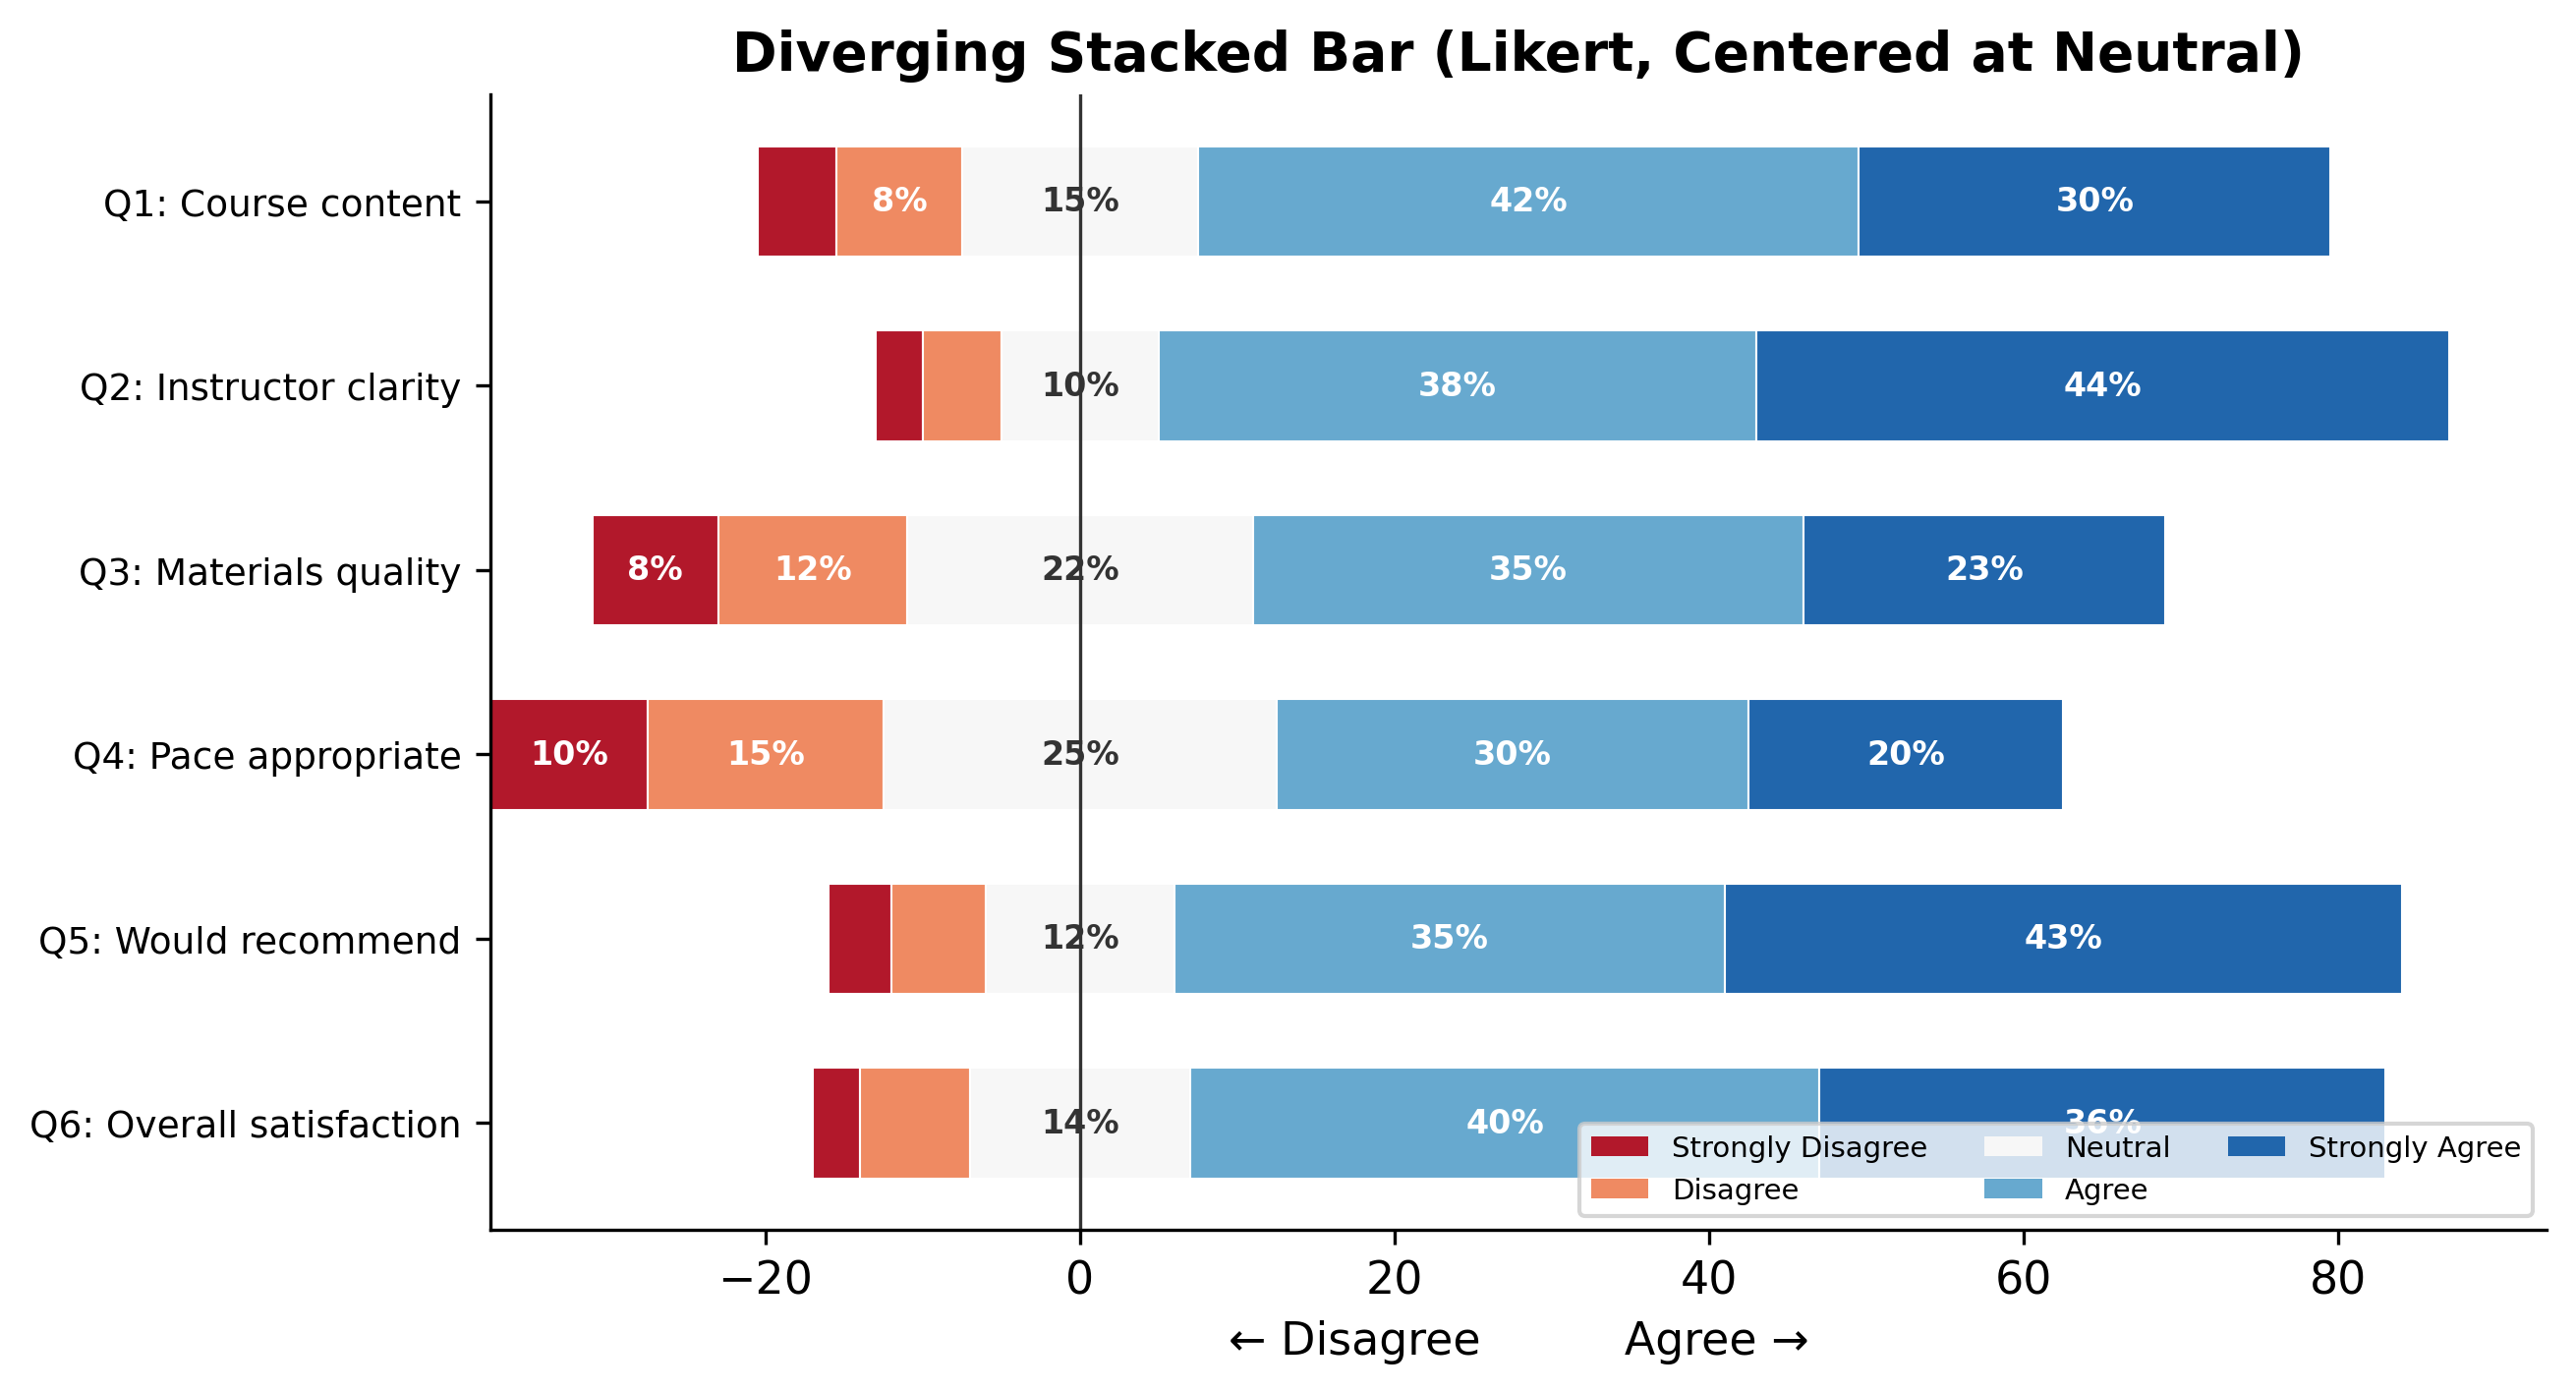
\includegraphics[width=\textwidth]{m3_4_diverging_stacked.png}
\begin{exampleblock}{Data Insight}
    \scriptsize The \texttt{likert} R package is purpose-built: \texttt{plot(lik, centered=TRUE)} produces the diverging layout with proper centering, percentage labels, and color scheme.
\end{exampleblock}
\end{column}
\end{columns}
\end{frame}

% ── 97 ──
\begin{frame}[fragile]{Diverging Stacked Bar --- \Python}\smark{97/300}
\begin{columns}[T]
\begin{column}{0.55\textwidth}
\begin{lstlisting}[style=Pystyle]
# Manual diverging bar in matplotlib
colors = ["#B2182B","#EF8A62",
    "#F7F7F7","#67A9CF","#2166AC"]

for qi in range(n_questions):
    row = data[qi]  # percentages
    # Center at neutral midpoint
    neg = row[0]+row[1]+row[2]/2
    x_start = -neg
    for li, (val, c) in enumerate(
        zip(row, colors)):
        ax.barh(qi, val,
            left=x_start,
            height=0.6, color=c)
        x_start += val
ax.axvline(0, color="#333", lw=0.8)

# pip install plot-likert
import plot_likert
plot_likert.plot_likert(df,
    plot_percentage=True,
    bar_labels=True)
\end{lstlisting}
\end{column}
\begin{column}{0.42\textwidth}
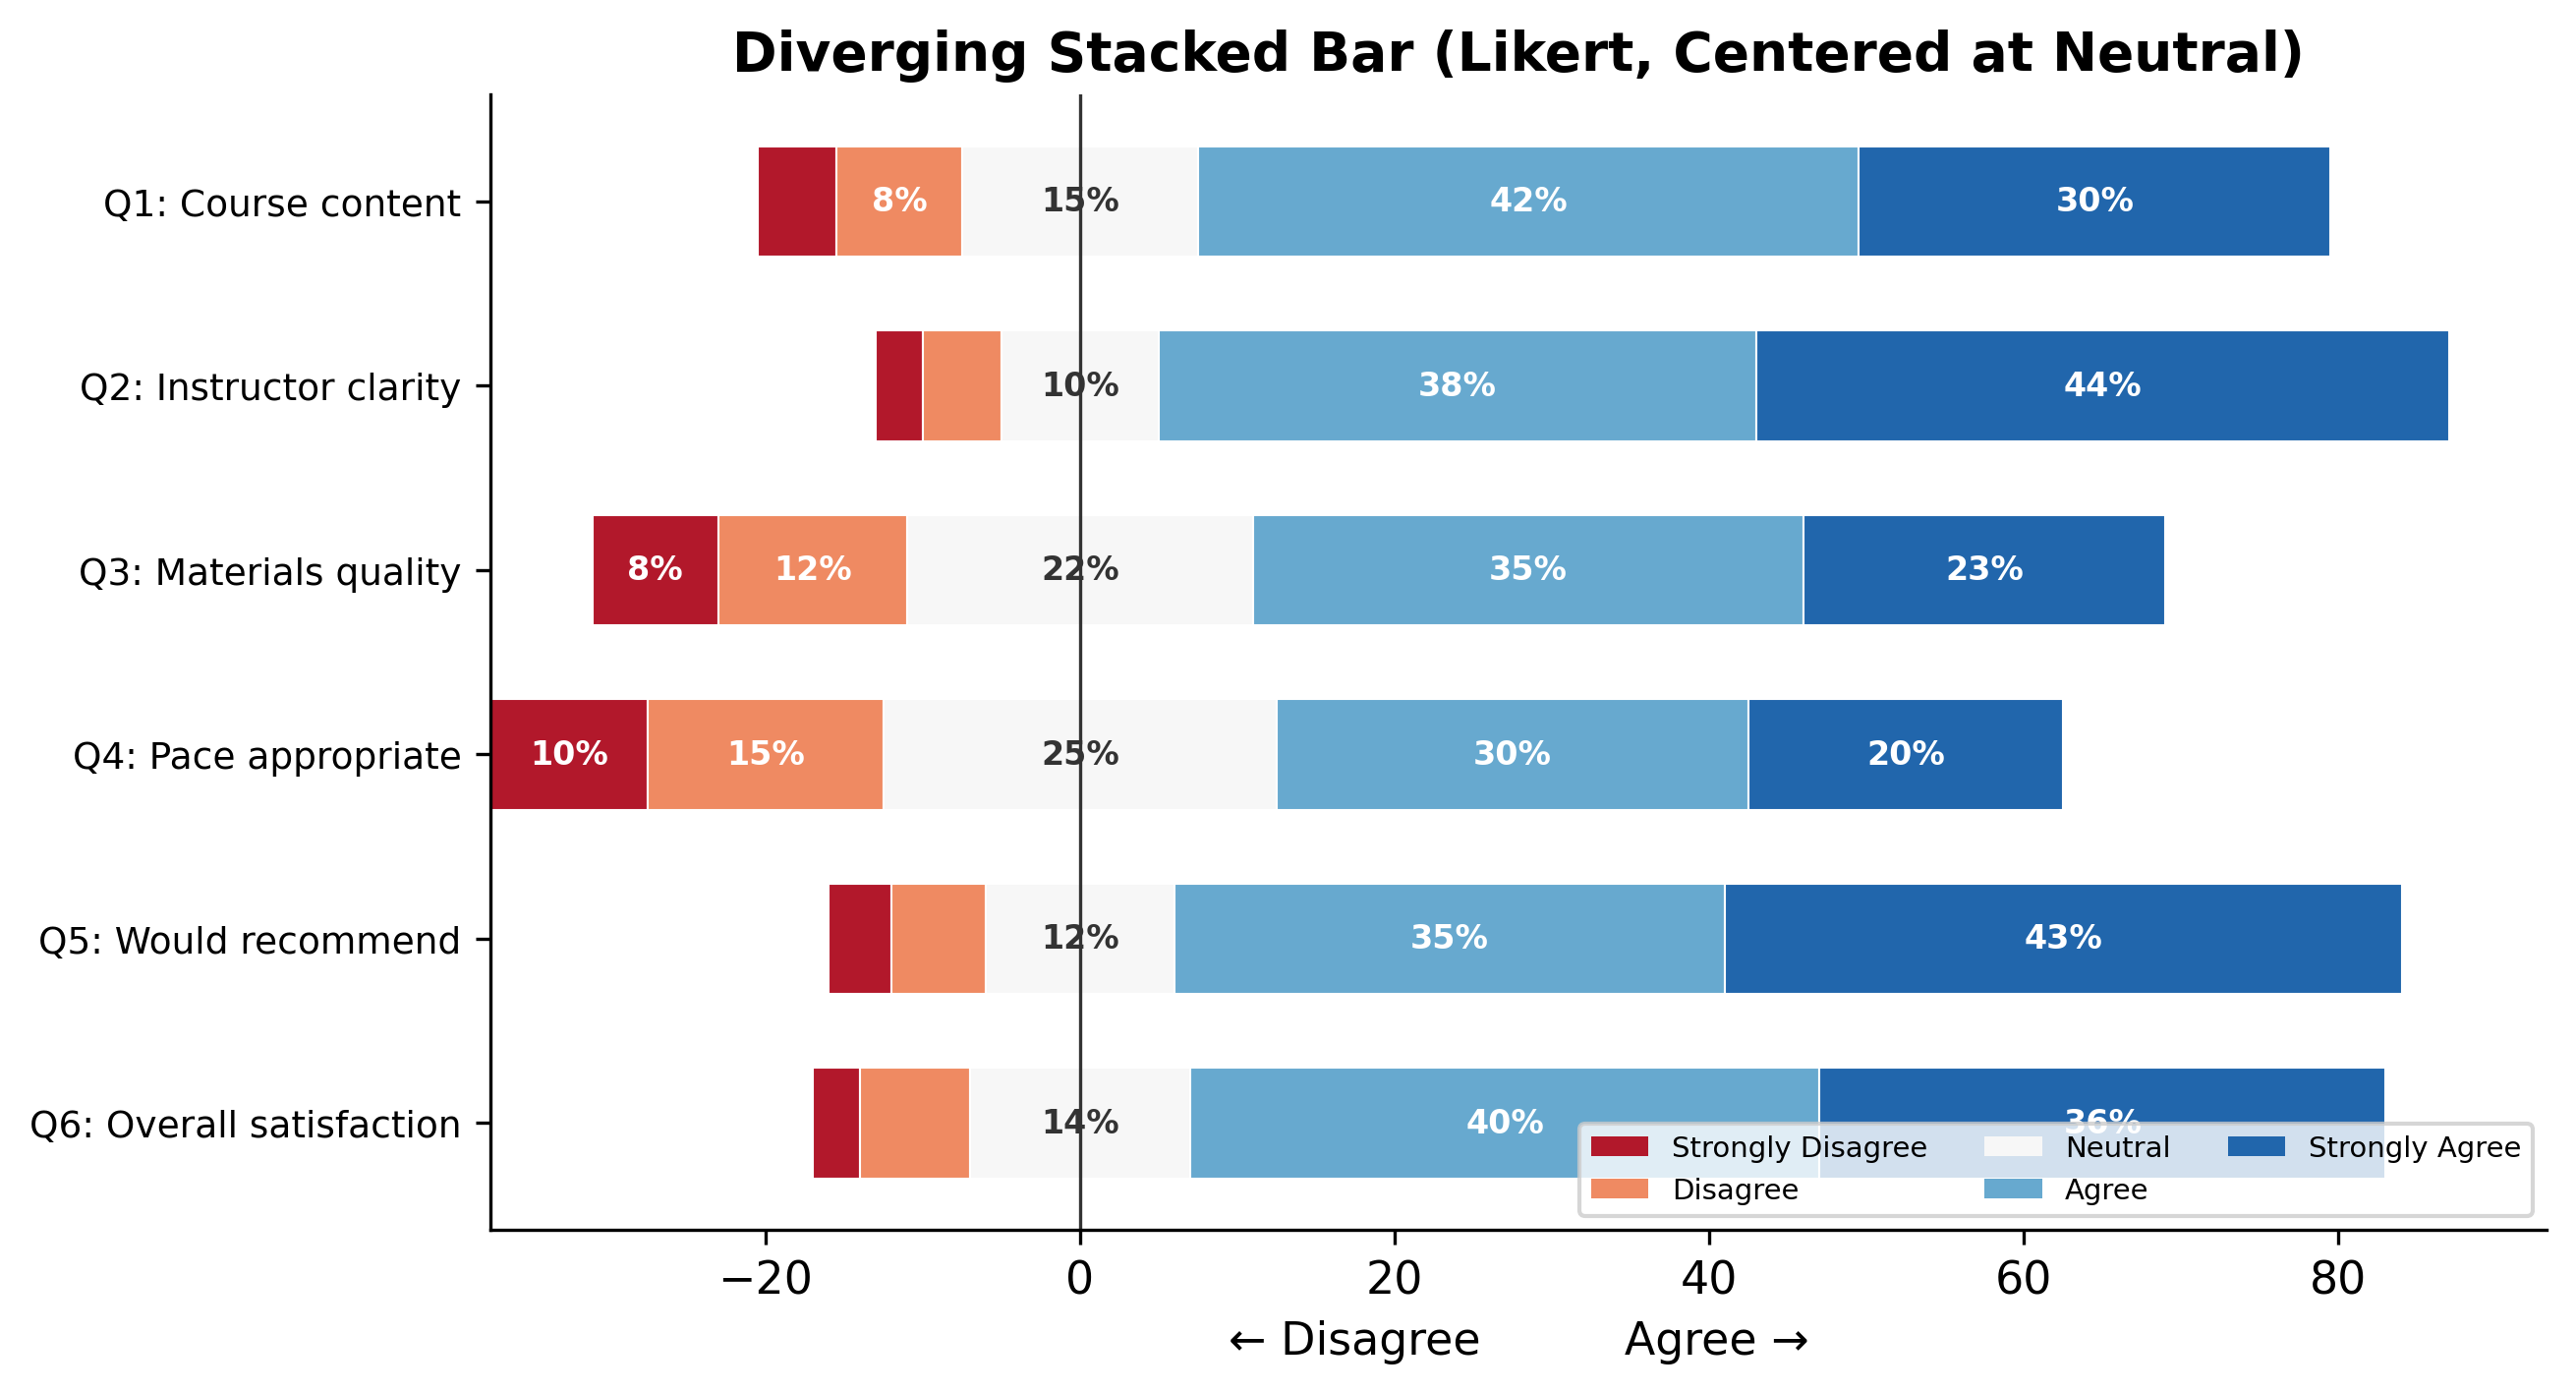
\includegraphics[width=\textwidth]{m3_4_diverging_stacked.png}
\begin{alertblock}{Pro-Tip}
    \scriptsize The \texttt{plot-likert} PyPI package automates the diverging layout. For full control, compute the centering offset manually: $\text{offset} = \text{SD}\% + \text{D}\% + \text{N}\%/2$.
\end{alertblock}
\end{column}
\end{columns}
\end{frame}

% ── 98 ──
\begin{frame}{Even vs.\ Odd Point Scales}
\smark{98/300}
\begin{columns}[T]
\begin{column}{0.50\textwidth}
    \textbf{Odd (5, 7-point):}
    \begin{itemize}
        \item Has a true neutral midpoint
        \item Diverging bar splits neutral at center
        \item Allows ``no opinion'' without forcing
    \end{itemize}
    \vspace{0.2cm}
    \textbf{Even (4, 6-point):}
    \begin{itemize}
        \item No neutral option (``forced choice'')
        \item Diverging bar splits between the two middle categories
        \item Prevents ``fence-sitting''
    \end{itemize}
\end{column}
\begin{column}{0.47\textwidth}
\begin{alertblock}{Pro-Tip}
    \scriptsize For even-point scales (no neutral), center the diverging bar between the two middle response options. The left half is all disagree; the right half is all agree. No neutral segment to split.
\end{alertblock}
\vspace{0.1cm}
\begin{exampleblock}{Data Insight}
    \scriptsize Whether to include a neutral depends on the construct. For sensitive topics (politics, bias), forced choice reduces social desirability. For knowledge items, neutral may reflect genuine uncertainty.
\end{exampleblock}
\end{column}
\end{columns}
\end{frame}

% ── 99 ──
\begin{frame}{Net Scores: Agree $-$ Disagree}
\smark{99/300}
\centering
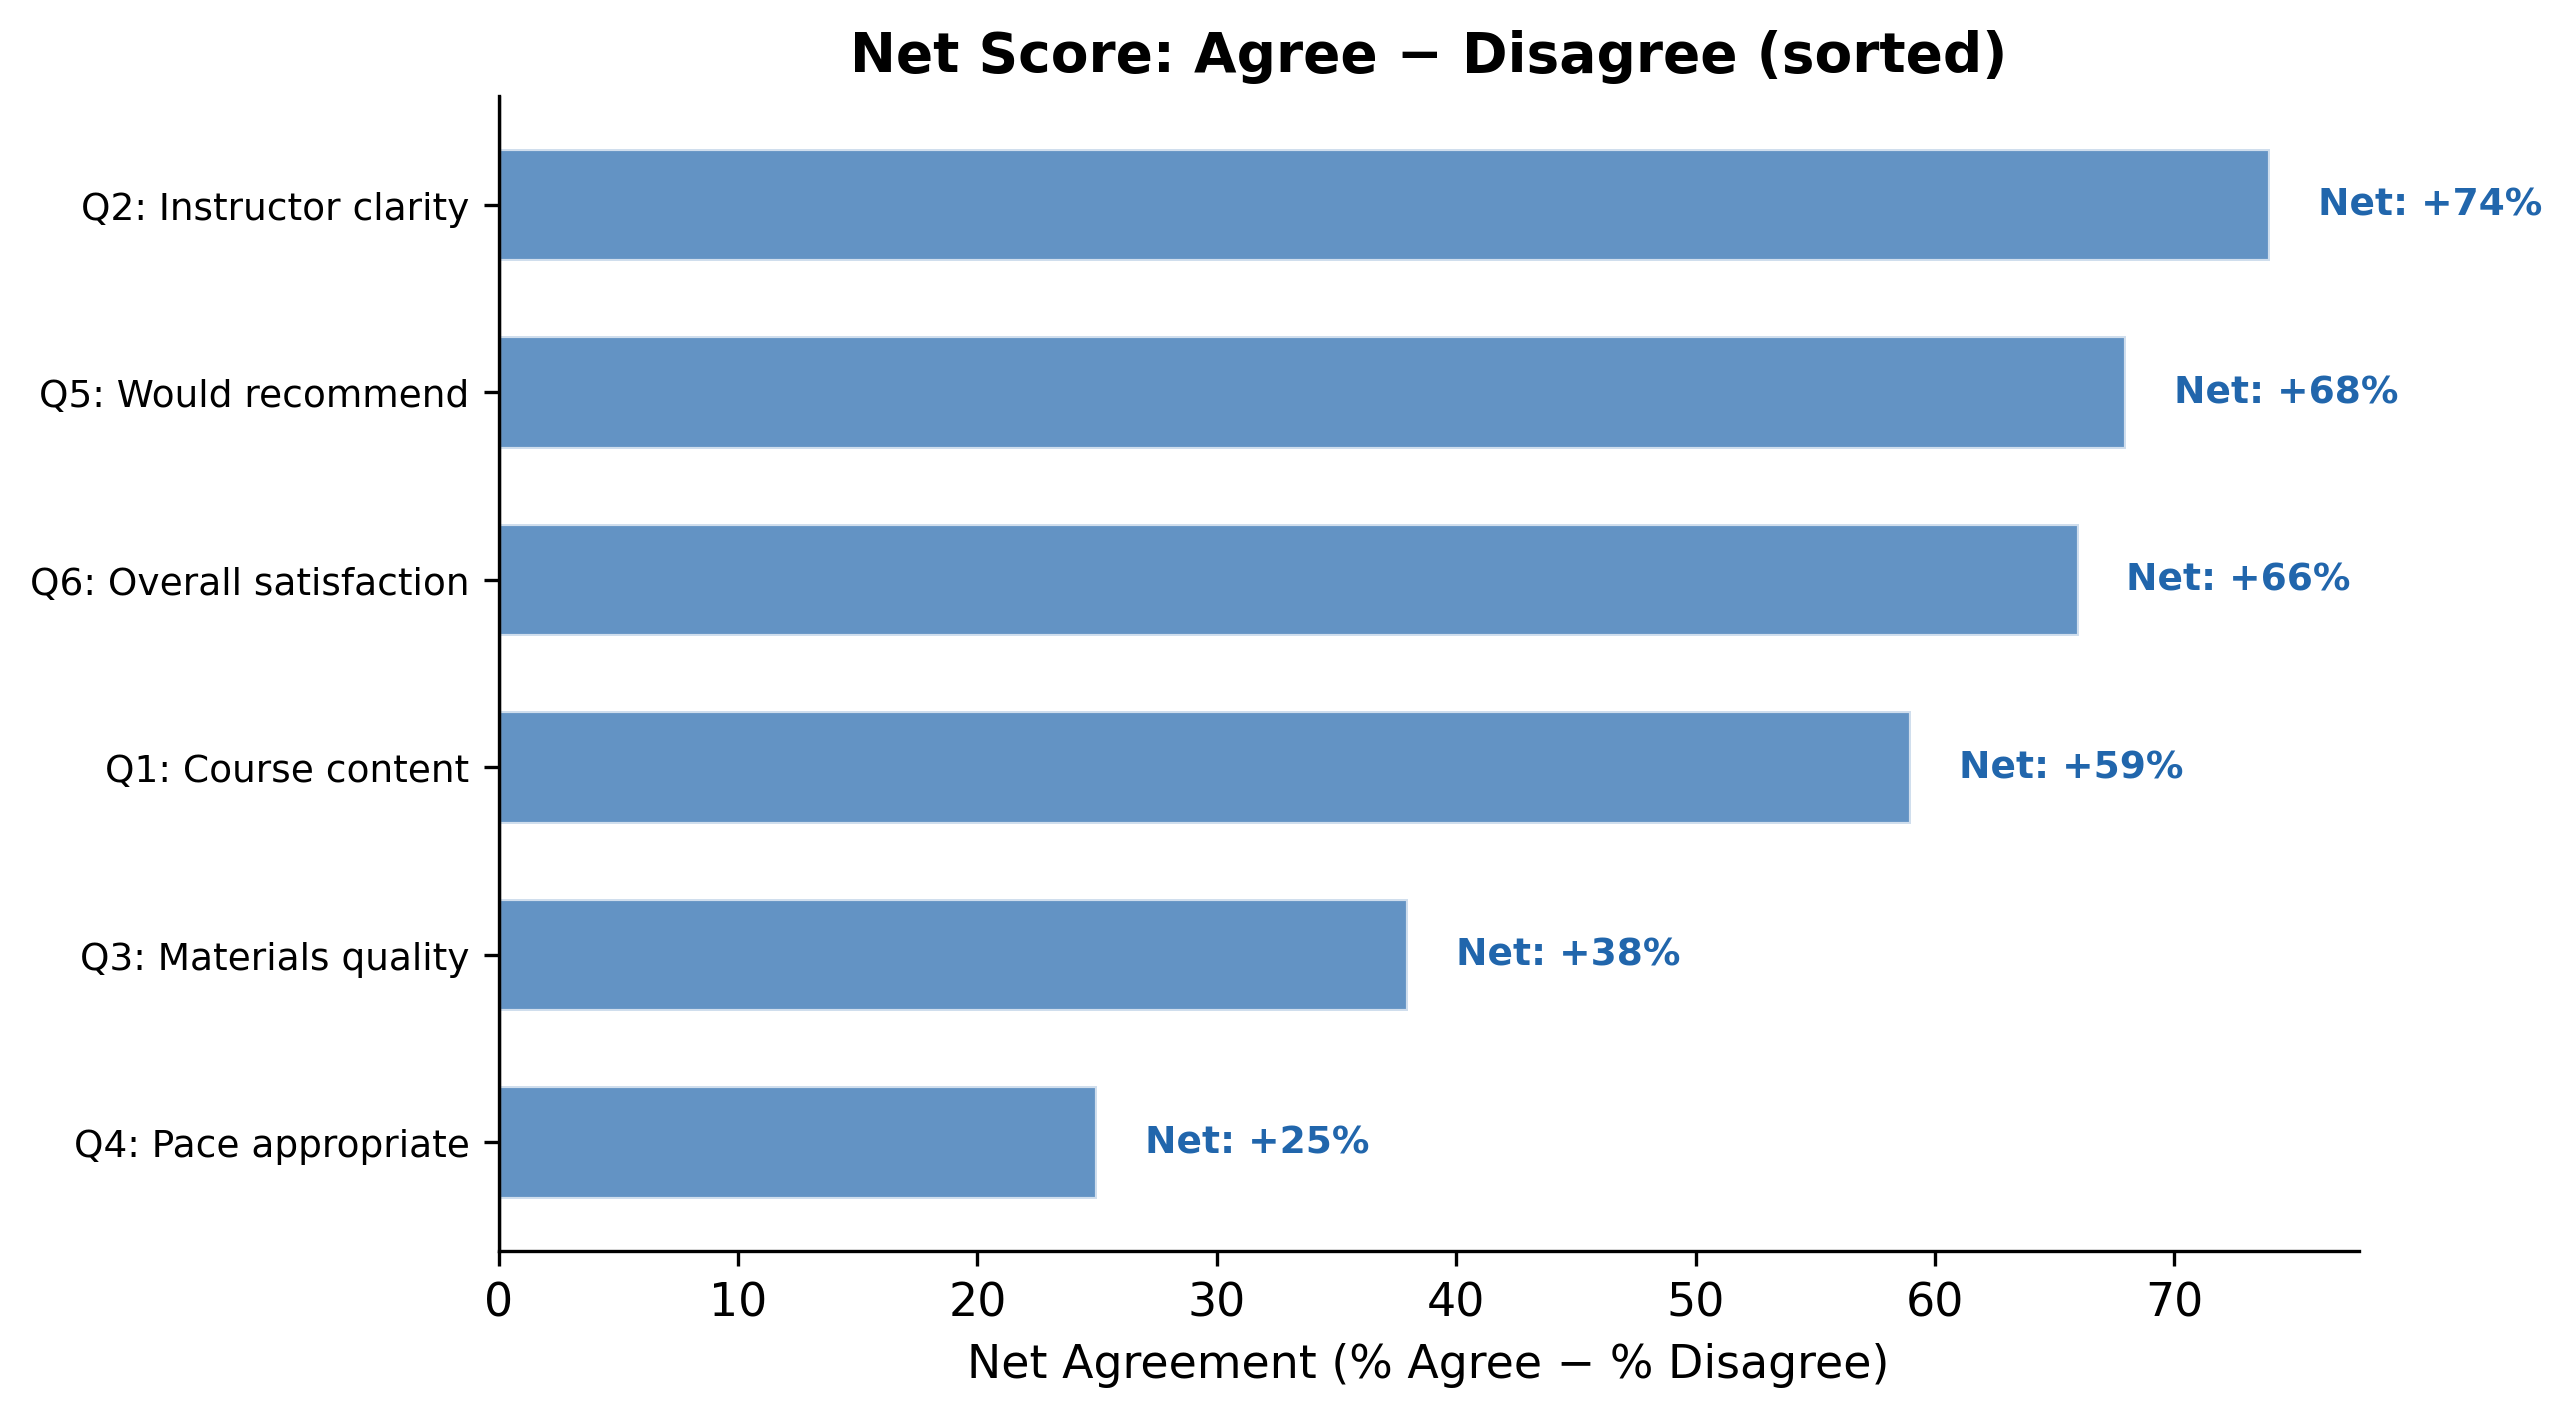
\includegraphics[width=0.72\textwidth]{m3_4_net_score.png}

\vspace{0.2cm}
\begin{columns}[T]
\begin{column}{0.48\textwidth}
\begin{itemize}
    \item Net = (Agree + SA) $-$ (Disagree + SD)
    \item Collapses 5 levels to one number
    \item Positive = more agreement than disagreement
    \item Sort by net score for instant ranking
    \item Good for executive summaries
\end{itemize}
\end{column}
\begin{column}{0.48\textwidth}
\begin{alertblock}{Pro-Tip}
    \scriptsize Net scores discard the distribution shape. A net of +50 could be 60\% Agree / 10\% Disagree (consensus) or 70\% SA / 20\% SD (polarized). \textbf{Always pair the net score with the full diverging bar.}
\end{alertblock}
\end{column}
\end{columns}
\end{frame}

% ── 100 ──
\begin{frame}[fragile]{Net Score --- Code}\smark{100/300}
\begin{columns}[T]
\begin{column}{0.48\textwidth}
\begin{lstlisting}[style=Rstyle]
# Compute net score per question
likert_df <- likert_df |>
  group_by(question) |>
  summarise(
    agree = mean(response %in%
      c("A","SA")) * 100,
    disagree = mean(response %in%
      c("SD","D")) * 100,
    net = agree - disagree)

# Plot
ggplot(likert_df,
  aes(fct_reorder(question, net),
      net, fill=net>0)) +
  geom_col() +
  coord_flip() +
  scale_fill_manual(
    values=c("#B2182B","#2166AC"))+
  geom_text(aes(label=sprintf(
    "%+.0f%%", net)),
    hjust=ifelse(
      likert_df$net>0,-0.1,1.1))+
  theme(legend.position="none")
\end{lstlisting}
\end{column}
\begin{column}{0.48\textwidth}
\begin{lstlisting}[style=Pystyle]
agree = data[:, 3] + data[:, 4]
disagree = data[:, 0] + data[:, 1]
net = agree - disagree
order = np.argsort(net)

for idx, qi in enumerate(order):
    c = "#2166AC" if net[qi] > 0 \
        else "#B2182B"
    ax.barh(idx, net[qi],
        color=c, height=0.6)
    ax.text(net[qi] + 2*np.sign(
        net[qi]), idx,
        f"{net[qi]:+.0f}%",
        va="center",
        fontweight="bold", color=c)
ax.axvline(0, color="#333", lw=0.8)
ax.set_yticks(range(len(questions)))
ax.set_yticklabels(
    [questions[i] for i in order])
\end{lstlisting}
\end{column}
\end{columns}
\end{frame}

% ── 101 ──
\begin{frame}{Likert Heatmap}
\smark{101/300}
\centering
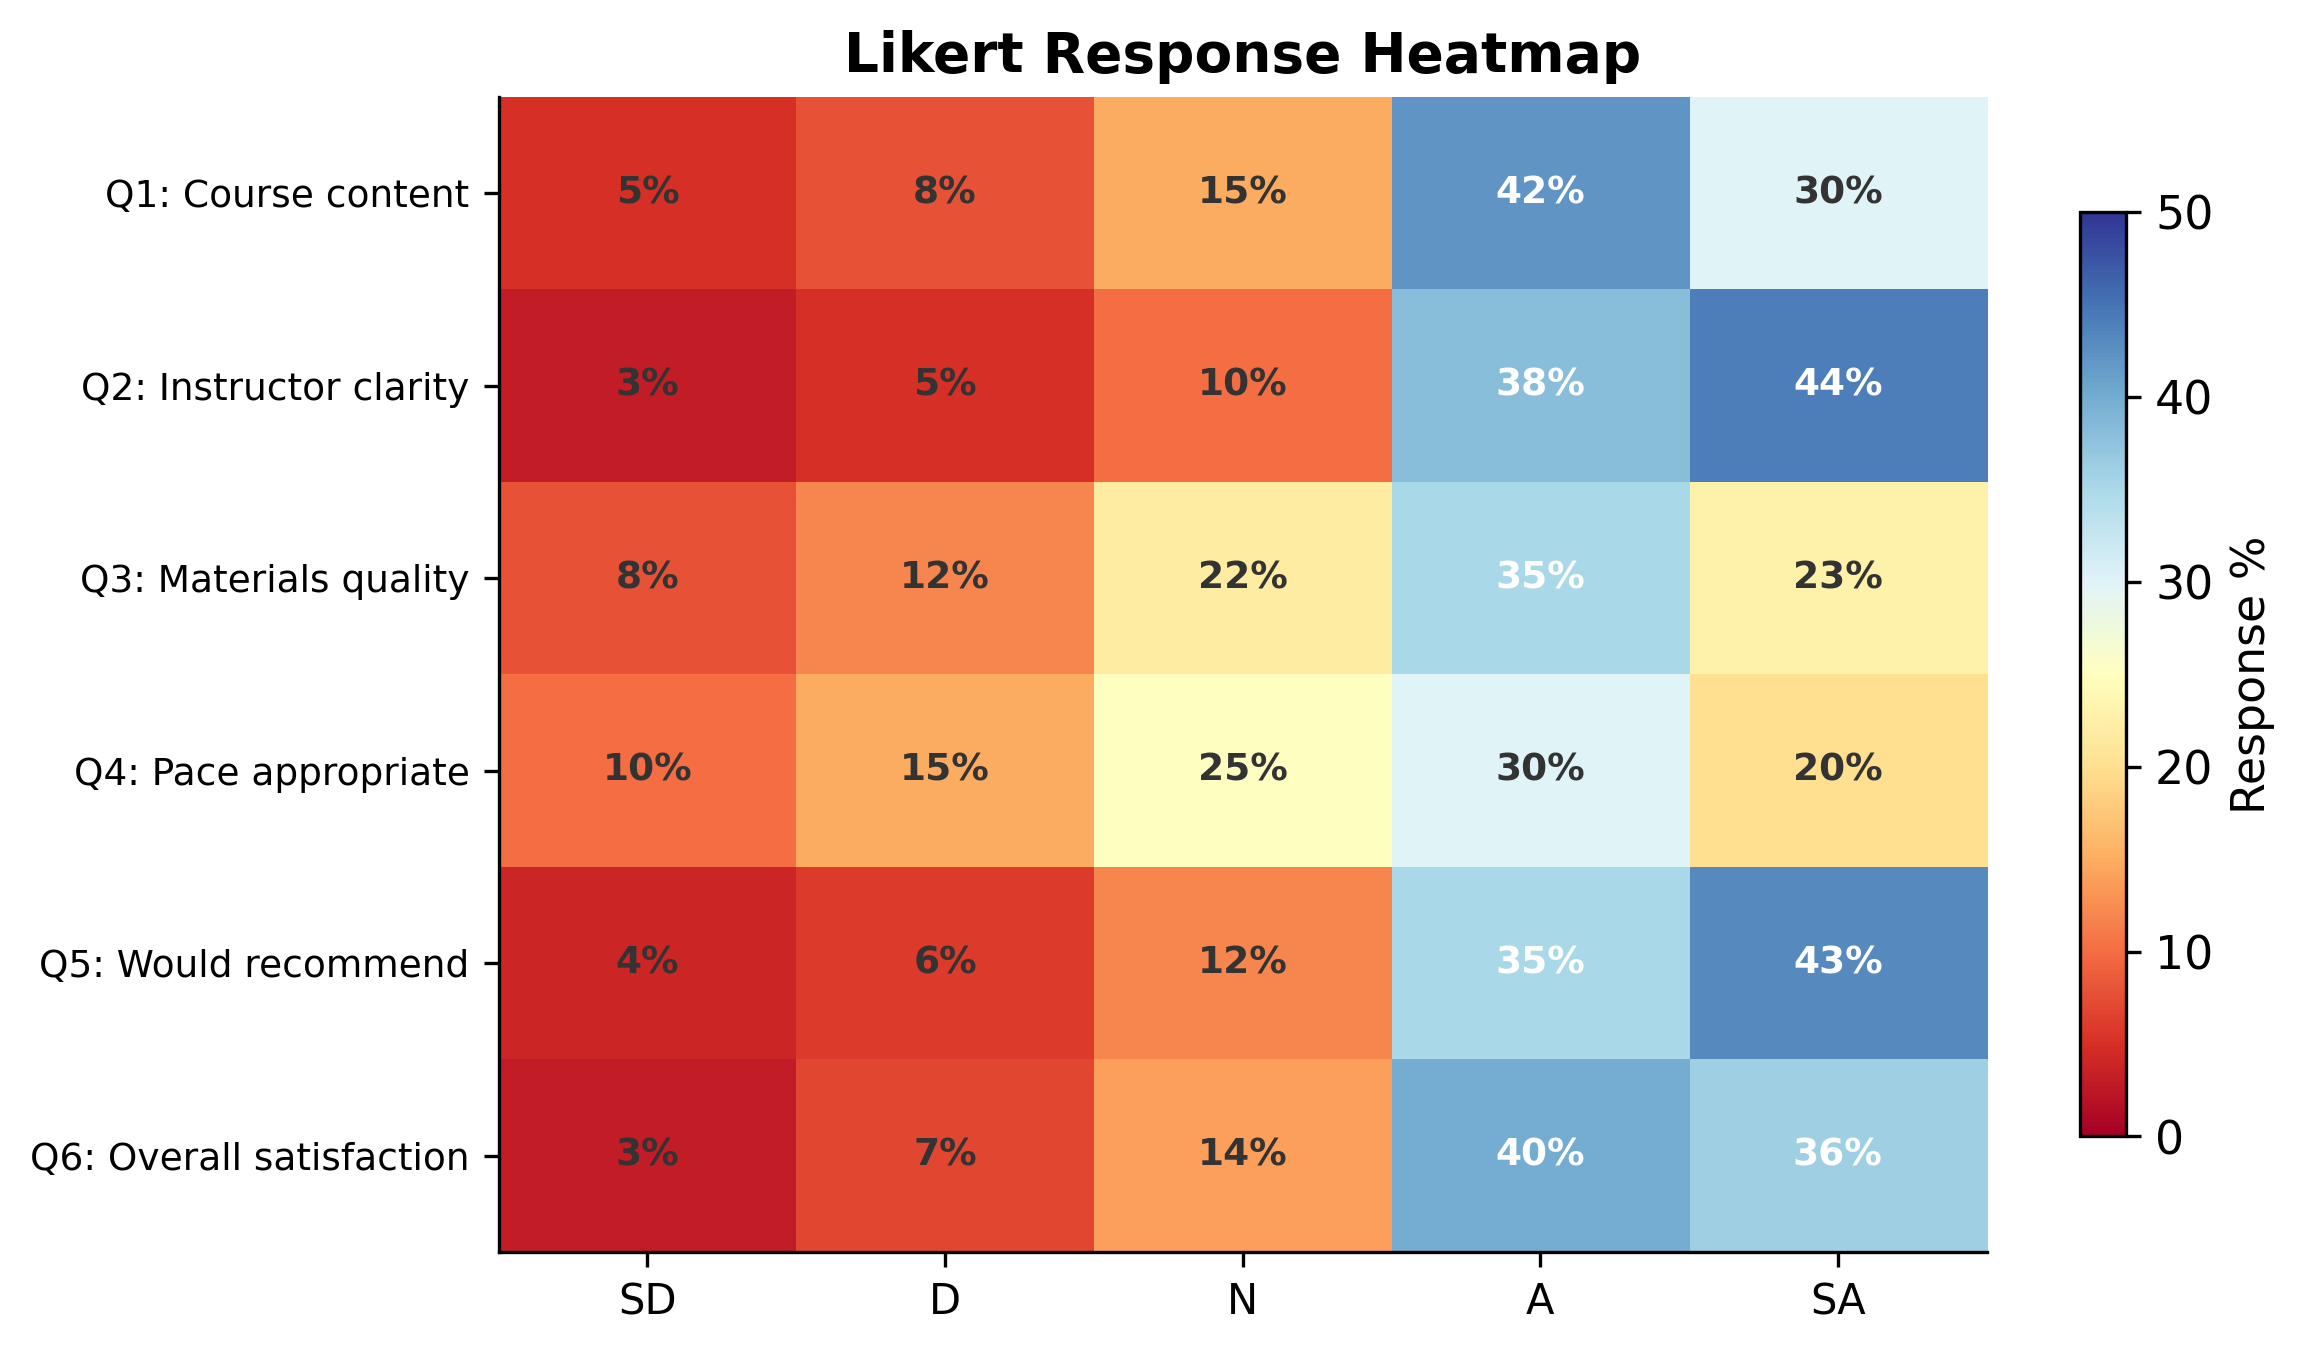
\includegraphics[width=0.68\textwidth]{m3_4_likert_heatmap.png}

\vspace{0.2cm}
\begin{columns}[T]
\begin{column}{0.48\textwidth}
\begin{itemize}
    \item Rows = questions; columns = response levels
    \item Cell color $\propto$ percentage
    \item Shows the \textbf{full response profile} for each question
    \item Useful for screening 20+ items quickly
    \item Reveals bimodal or polarized responses
\end{itemize}
\end{column}
\begin{column}{0.48\textwidth}
\begin{exampleblock}{Data Insight}
    \scriptsize Q4 (Pace) has the flattest profile: responses are spread across all levels. Q2 (Instructor) is strongly right-skewed. The heatmap reveals these distributional differences at a glance.
\end{exampleblock}
\end{column}
\end{columns}
\end{frame}

% ── 102 ──
\begin{frame}[fragile]{Likert Heatmap --- Code}\smark{102/300}
\begin{columns}[T]
\begin{column}{0.48\textwidth}
\begin{lstlisting}[style=Rstyle]
# Compute percentage per question
pct_df <- likert_df |>
  group_by(question, response) |>
  summarise(n=n()) |>
  mutate(pct = n/sum(n)*100)

# Heatmap
ggplot(pct_df,
  aes(response, question,
      fill=pct)) +
  geom_tile(color="white") +
  geom_text(aes(
    label=sprintf("%.0f%%",pct)),
    size=3) +
  scale_fill_distiller(
    palette="RdYlBu",
    direction=1) +
  theme_minimal()
\end{lstlisting}
\end{column}
\begin{column}{0.48\textwidth}
\begin{lstlisting}[style=Pystyle]
# data is n_questions x 5 matrix
df_heat = pd.DataFrame(data,
    index=questions,
    columns=["SD","D","N","A","SA"])

sns.heatmap(df_heat,
    annot=True, fmt=".0f",
    cmap="RdYlBu",
    linewidths=0.5,
    cbar_kws={"label":"Response %"})

# Add "%" to annotations
for t in ax.texts:
    t.set_text(t.get_text() + "%")
\end{lstlisting}
\vspace{0.1cm}
\begin{alertblock}{Pro-Tip}
    \scriptsize Use \texttt{RdYlBu} (diverging) palette so that low response (SD) is red and high (SA) is blue, matching the semantic meaning. The neutral column should appear white/yellow.
\end{alertblock}
\end{column}
\end{columns}
\end{frame}

% ── 103 ──
\begin{frame}{Diverging Bar + Mean Score Panel}
\smark{103/300}
\centering
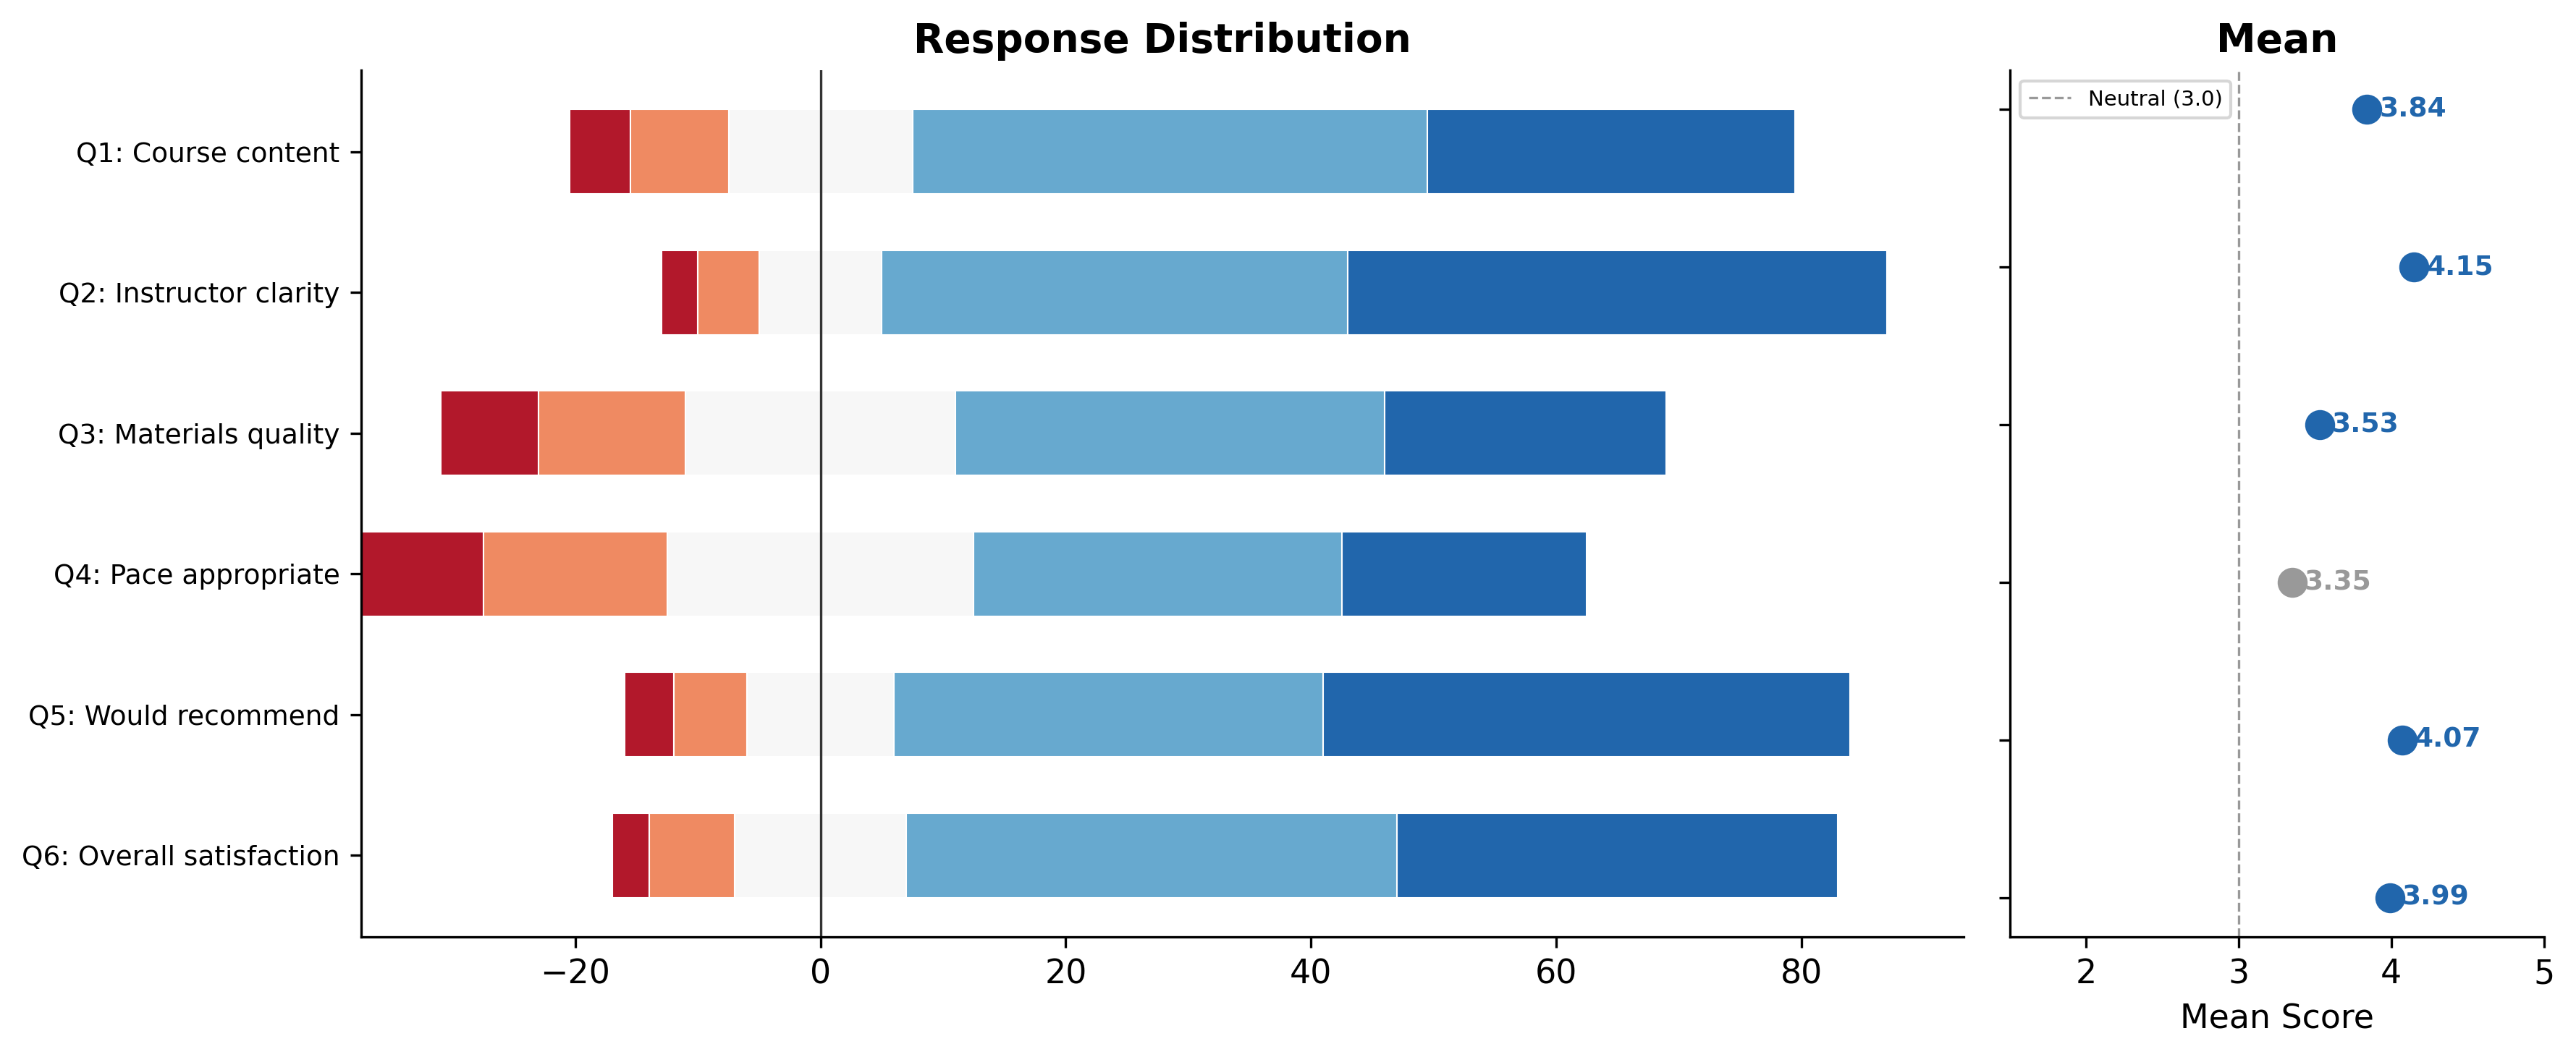
\includegraphics[width=0.85\textwidth]{m3_4_likert_with_mean.png}

\vspace{0.2cm}
\begin{exampleblock}{Data Insight}
    \scriptsize Left: the full distribution shows shape and spread. Right: the mean score summarizes each question as a single number. Together, they serve both the detail-oriented analyst and the time-pressed executive. Q2 and Q5 have the highest means ($>4.0$); Q4 is the weakest ($3.35$).
\end{exampleblock}
\end{frame}

% ── 104 ──
\begin{frame}[fragile]{Distribution + Mean Panel --- Code}\smark{104/300}
\begin{columns}[T]
\begin{column}{0.48\textwidth}
\begin{lstlisting}[style=Rstyle]
library(patchwork)

# Left: diverging bar
p1 <- plot(likert_obj,
  centered=TRUE) +
  theme(legend.position="none")

# Right: mean dot plot
mean_df <- data.frame(
  question=questions,
  mean=colMeans(
    apply(likert_data, 2,
          as.numeric)))
p2 <- ggplot(mean_df,
  aes(mean, fct_reorder(
    question, mean))) +
  geom_point(size=3,
    color="#2166AC") +
  geom_vline(xintercept=3,
    linetype="dashed") +
  xlim(1, 5)

p1 | p2  # patchwork layout
\end{lstlisting}
\end{column}
\begin{column}{0.48\textwidth}
\begin{lstlisting}[style=Pystyle]
fig, (ax1, ax2) = plt.subplots(
    1, 2, figsize=(12, 5),
    gridspec_kw={
        "width_ratios": [3, 1]})

# ax1: diverging stacked
# (same code as before)

# ax2: mean dot plot
mean_scores = np.sum(
    data * np.arange(1, 6),
    axis=1) / 100
for qi in range(n_q):
    ax2.scatter(mean_scores[qi],
        n_q-1-qi, s=80,
        color="#2166AC")
    ax2.text(mean_scores[qi]+0.08,
        n_q-1-qi,
        f"{mean_scores[qi]:.2f}",
        va="center", fontsize=9)
ax2.axvline(3, linestyle="--")
ax2.set_xlim(1.5, 5)
\end{lstlisting}
\end{column}
\end{columns}
\end{frame}

% ── 105 ──
\begin{frame}{Net Promoter Score (NPS) Visualization}
\smark{105/300}
\centering
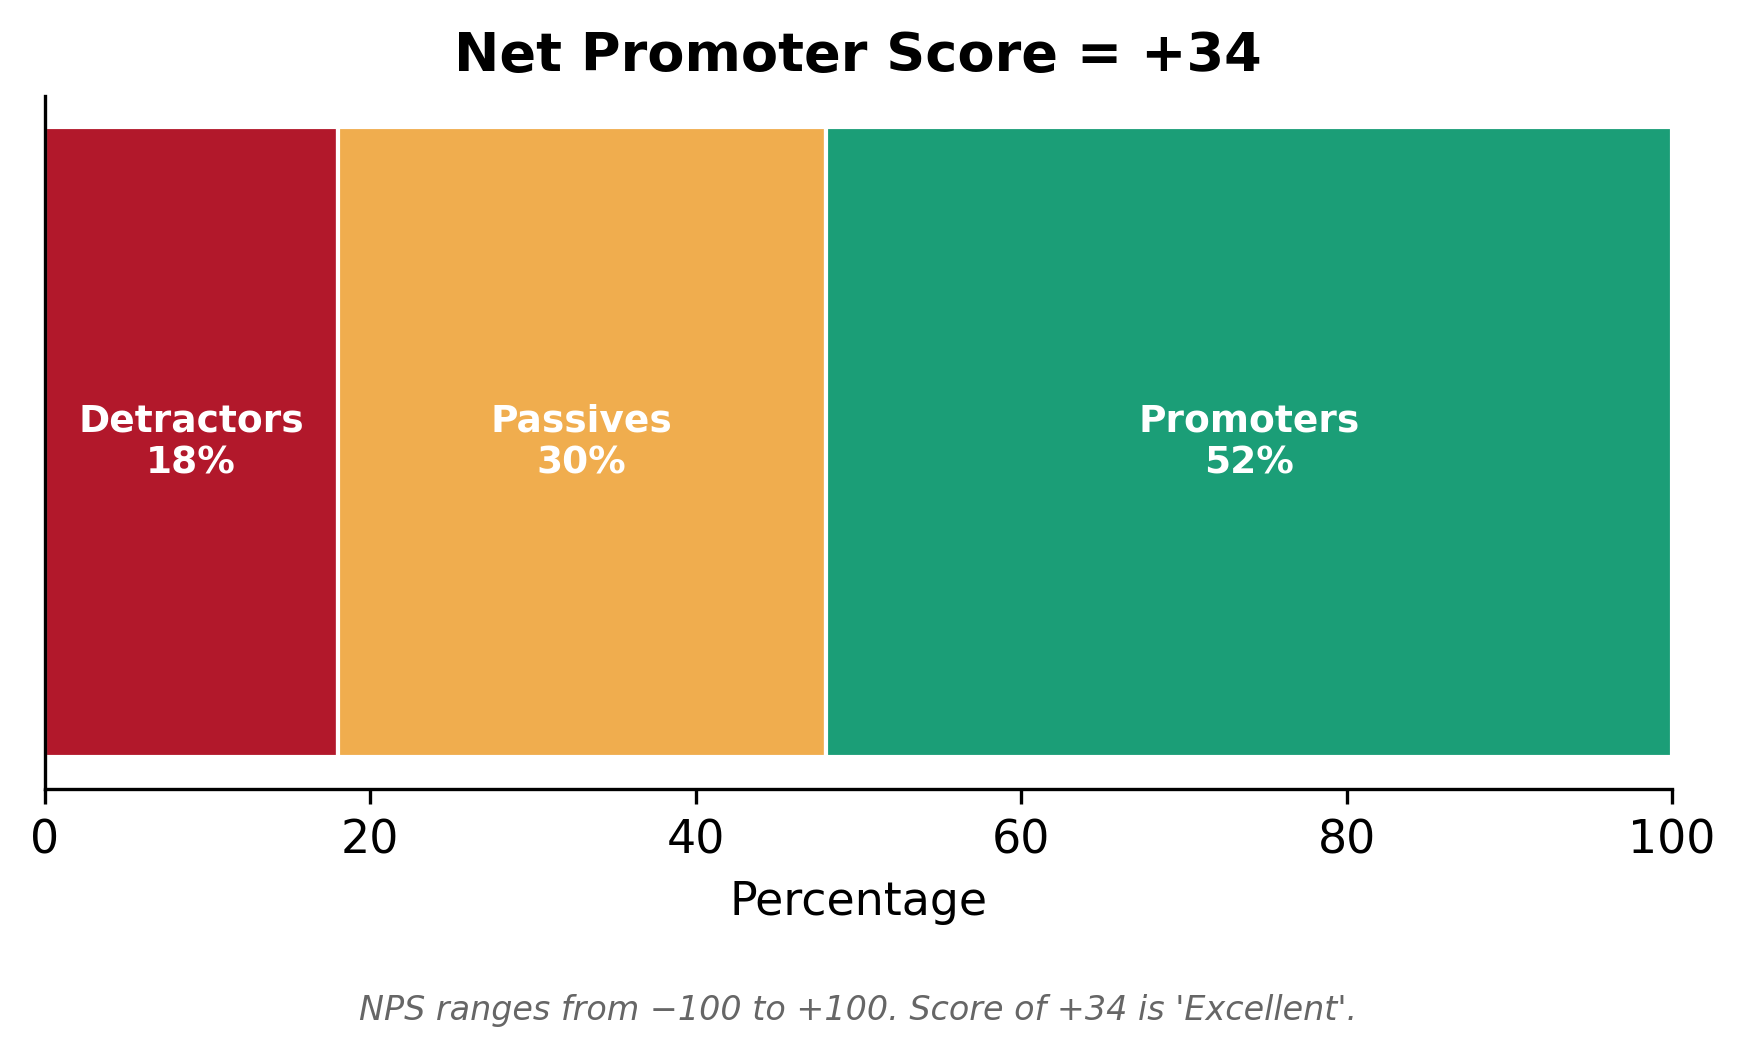
\includegraphics[width=0.72\textwidth]{m3_4_nps.png}

\vspace{0.2cm}
\begin{columns}[T]
\begin{column}{0.48\textwidth}
\begin{itemize}
    \item 0--10 scale: ``How likely to recommend?''
    \item 0--6 = Detractors; 7--8 = Passives; 9--10 = Promoters
    \item NPS = \%Promoters $-$ \%Detractors
    \item Range: $-100$ to $+100$
    \item $>50$ = Excellent; $>70$ = World-class
\end{itemize}
\end{column}
\begin{column}{0.48\textwidth}
\begin{alertblock}{Pro-Tip}
    \scriptsize NPS is essentially a net score on a collapsed 3-point scale. The same visualization principles apply: show the full distribution (Detractors/Passives/Promoters) alongside the headline number.
\end{alertblock}
\end{column}
\end{columns}
\end{frame}

% ── 106 ──
\begin{frame}[fragile]{NPS Visualization --- Code}\smark{106/300}
\begin{columns}[T]
\begin{column}{0.48\textwidth}
\begin{lstlisting}[style=Rstyle]
# Compute NPS
nps_df <- survey |>
  mutate(segment = case_when(
    score <= 6 ~ "Detractor",
    score <= 8 ~ "Passive",
    TRUE ~ "Promoter"))

nps <- mean(nps_df$segment ==
  "Promoter")*100 -
  mean(nps_df$segment ==
  "Detractor")*100

# Stacked bar
ggplot(nps_df,
  aes(x=1, fill=segment)) +
  geom_bar(position="fill",
    width=0.5) +
  coord_flip() +
  scale_fill_manual(values=c(
    "#B2182B","#F0AD4E","#1B9E77"))+
  labs(title=sprintf(
    "NPS = %+d", round(nps))) +
  theme_void()
\end{lstlisting}
\end{column}
\begin{column}{0.48\textwidth}
\begin{lstlisting}[style=Pystyle]
# Compute NPS
det = (scores <= 6).mean() * 100
pas = ((scores > 6) &
       (scores <= 8)).mean() * 100
pro = (scores >= 9).mean() * 100
nps = pro - det

# Stacked horizontal bar
ax.barh(0, det, color="#B2182B",
    label=f"Detractors {det:.0f}%")
ax.barh(0, pas, left=det,
    color="#F0AD4E",
    label=f"Passives {pas:.0f}%")
ax.barh(0, pro, left=det+pas,
    color="#1B9E77",
    label=f"Promoters {pro:.0f}%")
ax.set_title(f"NPS = {nps:+.0f}")
ax.legend(loc="lower center")
\end{lstlisting}
\end{column}
\end{columns}
\end{frame}

% ── 107 ──
\begin{frame}{Color Palettes for Likert Data}
\smark{107/300}
\centering\small
\begin{tabular}{@{}lll@{}}
    \toprule
    \textbf{Scale Points} & \textbf{Palette} & \textbf{Notes} \\
    \midrule
    5-point (with neutral)  & RdBu or BrBG (diverging) & Grey/white for neutral \\
    7-point (with neutral)  & RdYlBu (7 colors)         & Yellow for neutral \\
    4-point (no neutral)    & RdBu (4 steps)             & Split at center \\
    Agreement only          & Sequential blues            & Light to dark \\
    NPS (3 segments)        & Red / yellow / green        & Traffic-light intuition \\
    \bottomrule
\end{tabular}

\vspace{0.3cm}
\begin{alertblock}{Pro-Tip}
    \scriptsize \texttt{RColorBrewer::brewer.pal(5, "RdBu")} gives the exact 5-color diverging palette. In Python: \texttt{sns.color\_palette("RdBu", 5)}. The neutral midpoint should always be the lightest or most desaturated color.
\end{alertblock}
\end{frame}

% ── 108 ──
\begin{frame}{Multiple Likert Batteries: Grouped Panels}
\smark{108/300}
\begin{columns}[T]
\begin{column}{0.50\textwidth}
\begin{itemize}
    \item Surveys often have 3--5 \textbf{constructs}, each with 3--8 items
    \item Group items by construct with horizontal separators or faceting
    \item Add a \textbf{construct header} (bold label) above each group
    \item Sort within each group by net score or mean
\end{itemize}
\end{column}
\begin{column}{0.47\textwidth}
\begin{alertblock}{Pro-Tip}
    \scriptsize In R: \texttt{facet\_grid(construct \textasciitilde\ ., scales="free\_y", space="free\_y")} creates grouped panels with proportional heights. In Python: use \texttt{plt.subplots()} with one subplot per construct.
\end{alertblock}
\vspace{0.1cm}
\begin{exampleblock}{Data Insight}
    \scriptsize For large surveys (30+ items), the heatmap is more compact than the diverging bar. Use the heatmap for screening, then the diverging bar for the 6--8 items you want to present in detail.
\end{exampleblock}
\end{column}
\end{columns}
\end{frame}

% ── 109 ──
\begin{frame}{Handling ``Don't Know'' and Missing Responses}
\smark{109/300}
\begin{columns}[T]
\begin{column}{0.50\textwidth}
\begin{itemize}
    \item ``Don't Know'' (DK) is \textbf{not} a Likert level --- it is non-response
    \item Do not place DK on the diverging bar (it is not between agree and disagree)
    \item Options: (a) exclude DK and note the valid $n$; (b) show DK as a separate segment at the end; (c) annotate ``DK: 12\%'' next to the bar
    \item Always report the valid $n$ per question
\end{itemize}
\end{column}
\begin{column}{0.47\textwidth}
\begin{alertblock}{Pro-Tip}
    \scriptsize If DK exceeds 20\% for a question, the question is problematic (unclear wording, irrelevant to respondents). Flag it for revision rather than quietly excluding the non-responses.
\end{alertblock}
\vspace{0.1cm}
\begin{exampleblock}{Data Insight}
    \scriptsize The \texttt{likert} R package can handle DK responses separately. Set the ``Don't Know'' level to \texttt{NA} and use \texttt{na.rm=TRUE}; the package adjusts percentages to the valid base.
\end{exampleblock}
\end{column}
\end{columns}
\end{frame}

% ── 110 ──
\begin{frame}{Likert Item Analysis: Reliability and Validity}
\smark{110/300}
\begin{columns}[T]
\begin{column}{0.50\textwidth}
\begin{itemize}
    \item Cronbach's $\alpha$: internal consistency of a scale ($\alpha > 0.7$ acceptable)
    \item Item-total correlation: does each item correlate with the total? (drop if $r < 0.3$)
    \item Visualize: correlation heatmap of items within a construct (Module 2.6)
    \item Factor analysis biplot: do items cluster into expected factors? (Module 3.8)
\end{itemize}
\end{column}
\begin{column}{0.47\textwidth}
\begin{alertblock}{Pro-Tip}
    \scriptsize R: \texttt{psych::alpha(items)} computes Cronbach's $\alpha$ and item-total correlations. Python: \texttt{pingouin.cronbach\_alpha(items)}. Always report $\alpha$ in the methods section when using a Likert scale.
\end{alertblock}
\vspace{0.1cm}
\begin{exampleblock}{Data Insight}
    \scriptsize A low item-total correlation ($r < 0.3$) means the item is measuring something different from the rest of the scale. Visualize with a bar chart of item-total correlations, sorted, with a dashed line at 0.3.
\end{exampleblock}
\end{column}
\end{columns}
\end{frame}

% ── 111 ──
\begin{frame}[fragile]{Item Analysis --- Code}\smark{111/300}
\begin{columns}[T]
\begin{column}{0.48\textwidth}
\begin{lstlisting}[style=Rstyle]
library(psych)

# Cronbach's alpha
result <- alpha(item_matrix)
result$total$raw_alpha  # 0.85

# Item-total correlations
result$item.stats$r.drop

# Visualize
item_cors <- data.frame(
  item = names(result$item.stats
    $r.drop),
  r = result$item.stats$r.drop)
ggplot(item_cors,
  aes(fct_reorder(item, r), r)) +
  geom_col(fill="#2166AC") +
  geom_hline(yintercept=0.3,
    linetype="dashed", color=R) +
  coord_flip() + theme_minimal()
\end{lstlisting}
\end{column}
\begin{column}{0.48\textwidth}
\begin{lstlisting}[style=Pystyle]
import pingouin as pg

# Cronbach's alpha
alpha, ci = pg.cronbach_alpha(
    item_df)
print(f"alpha = {alpha:.3f}")

# Item-total correlations
total = item_df.sum(axis=1)
item_cors = {}
for col in item_df.columns:
    rest = total - item_df[col]
    item_cors[col] = \
        item_df[col].corr(rest)

# Bar chart
ax.barh(list(item_cors.keys()),
    list(item_cors.values()),
    color="#2166AC")
ax.axvline(0.3, linestyle="--",
    color="#B2182B")
\end{lstlisting}
\end{column}
\end{columns}
\end{frame}

% ── 112 ──
\begin{frame}{Top-Box and Bottom-Box Reporting}
\smark{112/300}
\begin{columns}[T]
\begin{column}{0.50\textwidth}
\begin{itemize}
    \item \textbf{Top-2 box}: \%Agree + \%Strongly Agree
    \item \textbf{Bottom-2 box}: \%Disagree + \%Strongly Disagree
    \item Common in market research and UX surveys
    \item Simpler than the full 5-level display but loses nuance
    \item Combine with net score for a compact summary
\end{itemize}
\end{column}
\begin{column}{0.47\textwidth}
\begin{exampleblock}{Data Insight}
    \scriptsize ``82\% of respondents agreed or strongly agreed with Q2'' is a top-2-box report. It collapses five levels to a binary, which is lossy but communicates clearly to non-technical stakeholders.
\end{exampleblock}
\vspace{0.1cm}
\begin{alertblock}{Pro-Tip}
    \scriptsize Visualize top-2 box as a simple horizontal bar chart sorted by percentage. Add the full diverging bar on a secondary panel for those who want the detail. This two-level approach serves both audiences.
\end{alertblock}
\end{column}
\end{columns}
\end{frame}

% ── 113 ──
\begin{frame}{Survey Visualization Design Principles}
\smark{113/300}
\centering\small
\begin{tabular}{@{}ll@{}}
    \toprule
    \textbf{Principle} & \textbf{Implementation} \\
    \midrule
    Diverging layout for Likert         & Center at neutral (or between middle levels for even scales) \\
    Color = semantic meaning             & Red = disagree, blue = agree, grey = neutral \\
    Sort by net score or mean            & Most positive at top (or bottom, consistently) \\
    Show full distribution               & Diverging bar, not just mean or top-box \\
    Report valid $n$                     & Annotate each row with sample size \\
    Group by construct                   & Horizontal separators or faceted panels \\
    Pair summary + detail                & Net score + diverging bar, or mean + distribution \\
    Handle DK separately                 & Do not include in the Likert bar \\
    \bottomrule
\end{tabular}
\end{frame}

% ── 114 ──
\begin{frame}{Likert Visualization Decision Guide}
\smark{114/300}
\centering\small
\begin{tabular}{@{}lll@{}}
    \toprule
    \textbf{Audience} & \textbf{Items} & \textbf{Best Display} \\
    \midrule
    Researchers          & 3--10     & Diverging stacked bar + mean \\
    Executives           & 3--10     & Net score bar (sorted) \\
    Large survey ($>20$) & 20--50    & Heatmap for screening \\
    Time series          & Any       & Mean $\pm$ CI over time \\
    Cross-group compare  & Any       & Faceted diverging bars by group \\
    Single question      & 1         & Spine plot or waffle \\
    \bottomrule
\end{tabular}

\vspace{0.3cm}
\begin{exampleblock}{Data Insight}
    \scriptsize For annual employee engagement surveys with 40+ items, use the heatmap as the ``dashboard view,'' then drill into diverging bars for the top-10 and bottom-10 items by net score.
\end{exampleblock}
\end{frame}

% ── 115 ──
\begin{frame}{Semantic Differential Scales}
\smark{115/300}
\begin{columns}[T]
\begin{column}{0.50\textwidth}
\begin{itemize}
    \item Bipolar adjective pairs: ``Boring --- Exciting'', ``Simple --- Complex''
    \item Respondents mark a position on a 7-point line between the poles
    \item Visualize with a \textbf{profile plot}: connected dots across items
    \item Multiple groups $\to$ overlaid profiles for comparison
\end{itemize}
\end{column}
\begin{column}{0.47\textwidth}
\begin{alertblock}{Pro-Tip}
    \scriptsize The semantic differential profile plot is essentially a \textbf{parallel coordinate plot} with the adjective pairs as axes. Each respondent (or group mean) is a line traversing the axes. Osgood, Suci, \& Tannenbaum (1957) pioneered this for measuring connotative meaning.
\end{alertblock}
\end{column}
\end{columns}
\end{frame}

% ── 116 ──
\begin{frame}[fragile]{Semantic Differential --- Code}\smark{116/300}
\begin{columns}[T]
\begin{column}{0.48\textwidth}
\begin{lstlisting}[style=Rstyle]
# Profile plot: mean per item
means <- survey |>
  group_by(item) |>
  summarise(m = mean(score))

ggplot(means, aes(m, fct_rev(item)))+
  geom_point(size=3,
    color="#2166AC") +
  geom_segment(aes(
    x=1, xend=m, yend=item),
    color="#2166AC", linewidth=1) +
  geom_vline(xintercept=4,
    linetype="dashed", color="#CCC")+
  scale_x_continuous(
    limits=c(1,7),
    breaks=1:7) +
  theme_minimal()
\end{lstlisting}
\end{column}
\begin{column}{0.48\textwidth}
\begin{lstlisting}[style=Pystyle]
items = ["Boring-Exciting",
    "Simple-Complex",
    "Cold-Warm",
    "Traditional-Modern"]
group_a = [5.2, 3.8, 4.5, 5.8]
group_b = [3.1, 5.5, 2.8, 4.2]

for vals, label, c in [
    (group_a, "Product A", "#2166AC"),
    (group_b, "Product B", "#B2182B")]:
    ax.plot(vals, range(len(items)),
        "o-", color=c, linewidth=2,
        markersize=8, label=label)
ax.set_yticks(range(len(items)))
ax.set_yticklabels(items)
ax.axvline(4, linestyle="--")
ax.set_xlim(1, 7)
ax.legend()
\end{lstlisting}
\end{column}
\end{columns}
\end{frame}

% ── 117 ──
\begin{frame}{Comparing Groups on Likert Items}
\smark{117/300}
\begin{columns}[T]
\begin{column}{0.50\textwidth}
\begin{itemize}
    \item \textbf{Faceted diverging bars}: one panel per group, shared scale
    \item \textbf{Overlaid mean dots}: group means on the same axis, different shapes/colors
    \item \textbf{Difference bar}: plot the \textbf{gap} between groups per item
    \item Statistical test: Mann--Whitney $U$ (ordinal) or $t$-test (if treating as interval)
\end{itemize}
\end{column}
\begin{column}{0.47\textwidth}
\begin{alertblock}{Pro-Tip}
    \scriptsize For group comparison, the \textbf{difference plot} (like Module 2.7's estimation plot) is more informative than side-by-side bars. Compute the difference in mean scores per item, with bootstrap CIs, and plot as a Cleveland dot plot.
\end{alertblock}
\end{column}
\end{columns}
\end{frame}

% ── 118 ──
\begin{frame}[fragile]{Group Comparison --- Code}\smark{118/300}
\begin{columns}[T]
\begin{column}{0.48\textwidth}
\begin{lstlisting}[style=Rstyle]
# Faceted diverging bars
plot(likert_obj) +
  facet_wrap(~group, ncol=1) +
  theme_minimal()

# Difference in means + CI
library(emmeans)
model <- lm(score ~ group*item,
  data=survey)
emm <- emmeans(model,
  pairwise ~ group | item)
plot(emm$contrasts) +
  geom_vline(xintercept=0,
    linetype="dashed")
\end{lstlisting}
\end{column}
\begin{column}{0.48\textwidth}
\begin{lstlisting}[style=Pystyle]
# Faceted diverging
fig, axes = plt.subplots(2, 1,
    figsize=(10, 8), sharex=True)
for ax, group in zip(axes,
    ["Control","Treatment"]):
    sub = data[data.group==group]
    # draw diverging bars on ax

# Difference dot plot
diffs = means_treatment - means_ctrl
ax.scatter(diffs, range(n_items))
ax.axvline(0, linestyle="--")
for i, d in enumerate(diffs):
    ax.text(d+0.05, i,
        f"{d:+.2f}", fontsize=8)
\end{lstlisting}
\end{column}
\end{columns}
\end{frame}

% ── 119 ──
\begin{frame}{Likert Over Time: Tracking Change}
\smark{119/300}
\begin{columns}[T]
\begin{column}{0.50\textwidth}
\begin{itemize}
    \item Same survey administered at multiple time points
    \item \textbf{Small-multiple diverging bars}: one panel per wave, vertically aligned
    \item \textbf{Line chart of mean scores}: trend over time with CI bands
    \item \textbf{Slope chart}: before/after for 2 waves
    \item Always use the same scale and color palette across waves
\end{itemize}
\end{column}
\begin{column}{0.47\textwidth}
\begin{alertblock}{Pro-Tip}
    \scriptsize For tracking: plot the \textbf{mean $\pm$ CI} per item over time as a line chart (Module 1.3 style). This reduces 5$\times$items$\times$waves data points to a readable trend. Supplement with the full diverging bar for the most recent wave.
\end{alertblock}
\end{column}
\end{columns}
\end{frame}

% ── 120 ──
\begin{frame}{Module 3.4 --- Key Takeaways}\smark{120/300}
\begin{enumerate}
    \item \textbf{Diverging stacked bars} are the standard for Likert data: centered at neutral.
    \item \textbf{Net scores} summarize agreement balance; always pair with the full distribution.
    \item \textbf{Heatmaps} screen large item batteries (20+ questions) at a glance.
    \item \textbf{Mean + distribution panel} serves both researchers and executives.
    \item \textbf{NPS} is a net score on a collapsed 3-point scale: same visualization principles apply.
    \item \textbf{Color palette = semantic}: red for disagree, blue for agree, grey for neutral.
\end{enumerate}
\end{frame}

% ── 121 ──
\begin{frame}{}\smark{121/300}
\centering\vspace{1.5cm}
{\Large\textbf{Module 3.4 Complete}}\\[0.5cm]
You can now visualize Likert scales with diverging stacked bars, net scores, heatmaps, mean panels, NPS gauges, and semantic differential profiles --- with proper centering, color semantics, and group comparisons.\\[0.5cm]
\textbf{Next:} Module 3.5 --- Correspondence Analysis and Biplots.
\end{frame}

% ═══════════════════════════════════════════════════════
%  MODULE 3.5 — Correspondence Analysis and Biplots
% ═══════════════════════════════════════════════════════
\section{Module 3.5 --- Correspondence Analysis and Biplots}

% ── 122 ──
\begin{frame}{Module 3.5 --- Roadmap}\smark{122/300}
\begin{enumerate}
    \item What is Correspondence Analysis (CA)?
    \item Row and column profiles
    \item The CA biplot: reading proximity as association
    \item Inertia: scree plot and dimensionality
    \item Contributions and quality of representation (cos$^2$)
    \item Multiple Correspondence Analysis (MCA)
    \item Supplementary points
    \item R and Python implementation
\end{enumerate}
\end{frame}

% ── 123 ──
\begin{frame}{What Is Correspondence Analysis?}
\smark{123/300}
\begin{columns}[T]
\begin{column}{0.50\textwidth}
\begin{itemize}
    \item A \textbf{dimension reduction} technique for contingency tables
    \item Analogous to PCA, but for categorical data
    \item Decomposes the $\chi^2$ distance between row/column profiles
    \item Projects rows and columns into a shared low-dimensional space
    \item Proximity on the biplot $\approx$ association in the table
\end{itemize}
\end{column}
\begin{column}{0.47\textwidth}
\begin{exampleblock}{Data Insight}
    \scriptsize CA answers: ``Which row categories are similar? Which column categories are similar? Which row categories are associated with which column categories?'' All in one display.
\end{exampleblock}
\vspace{0.1cm}
\begin{alertblock}{Pro-Tip}
    \scriptsize CA is to contingency tables what PCA is to correlation matrices. If you understand PCA (Workshop 5), CA follows the same logic with $\chi^2$ distances instead of Euclidean.
\end{alertblock}
\end{column}
\end{columns}
\end{frame}

% ── 124 ──
\begin{frame}{Row and Column Profiles}
\smark{124/300}
\centering
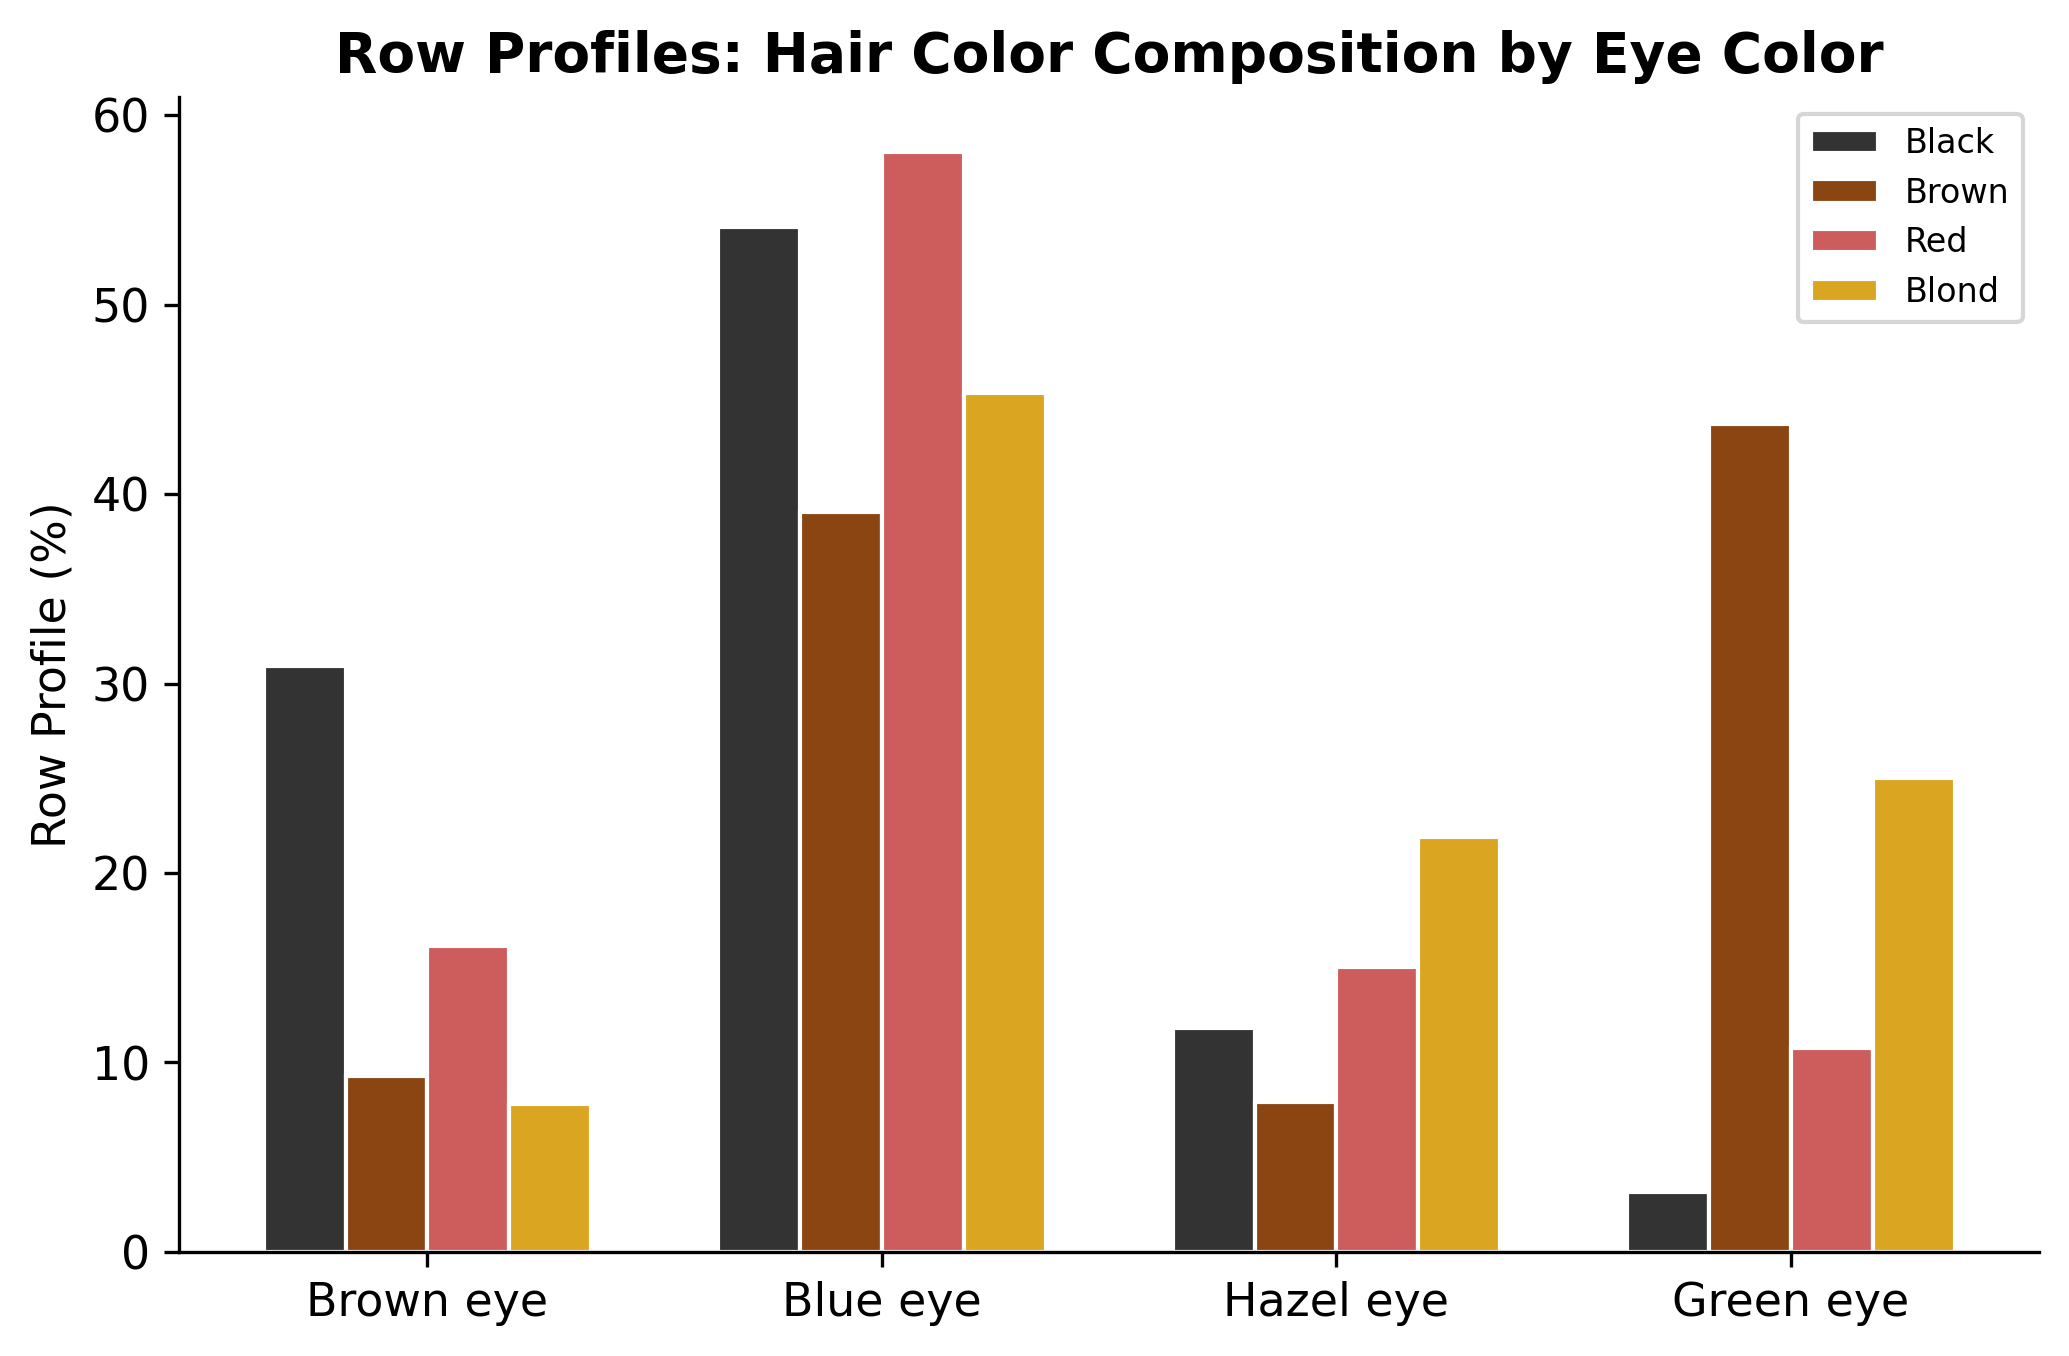
\includegraphics[width=0.72\textwidth]{m3_5_row_profiles.png}

\vspace{0.2cm}
\begin{columns}[T]
\begin{column}{0.48\textwidth}
\begin{itemize}
    \item \textbf{Row profile}: each row's distribution across columns (row-normalized to 100\%)
    \item \textbf{Column profile}: each column's distribution across rows
    \item If all profiles are identical $\to$ independence
    \item CA measures \textbf{how much profiles deviate} from the average
\end{itemize}
\end{column}
\begin{column}{0.48\textwidth}
\begin{exampleblock}{Data Insight}
    \scriptsize Brown-haired people are mostly green-eyed (rightmost bar). Black-haired people are disproportionately blue-eyed. The row profiles differ $\to$ hair and eye color are associated.
\end{exampleblock}
\end{column}
\end{columns}
\end{frame}

% ── 125 ──
\begin{frame}[fragile]{Row/Column Profiles --- Code}\smark{125/300}
\begin{columns}[T]
\begin{column}{0.48\textwidth}
\begin{lstlisting}[style=Rstyle]
ct <- as.table(matrix(...))

# Row profiles (each row sums to 1)
row_profiles <- prop.table(ct,
  margin = 1)

# Column profiles
col_profiles <- prop.table(ct,
  margin = 2)

# Average profile (centroid)
avg_row <- colSums(ct) / sum(ct)
avg_col <- rowSums(ct) / sum(ct)

# Visualize
barplot(t(row_profiles),
  beside=TRUE, legend=TRUE)
\end{lstlisting}
\end{column}
\begin{column}{0.48\textwidth}
\begin{lstlisting}[style=Pystyle]
ct = pd.crosstab(hair, eye)

# Row profiles
row_profiles = ct.div(
    ct.sum(axis=1), axis=0)

# Column profiles
col_profiles = ct.div(
    ct.sum(axis=0), axis=1)

# Average profile
avg_row = ct.sum(axis=0) / ct.sum()\
    .sum()

# Visualize
row_profiles.plot(kind="bar",
    stacked=False)
\end{lstlisting}
\end{column}
\end{columns}
\end{frame}

% ── 126 ──
\begin{frame}{The CA Biplot}
\smark{126/300}
\centering
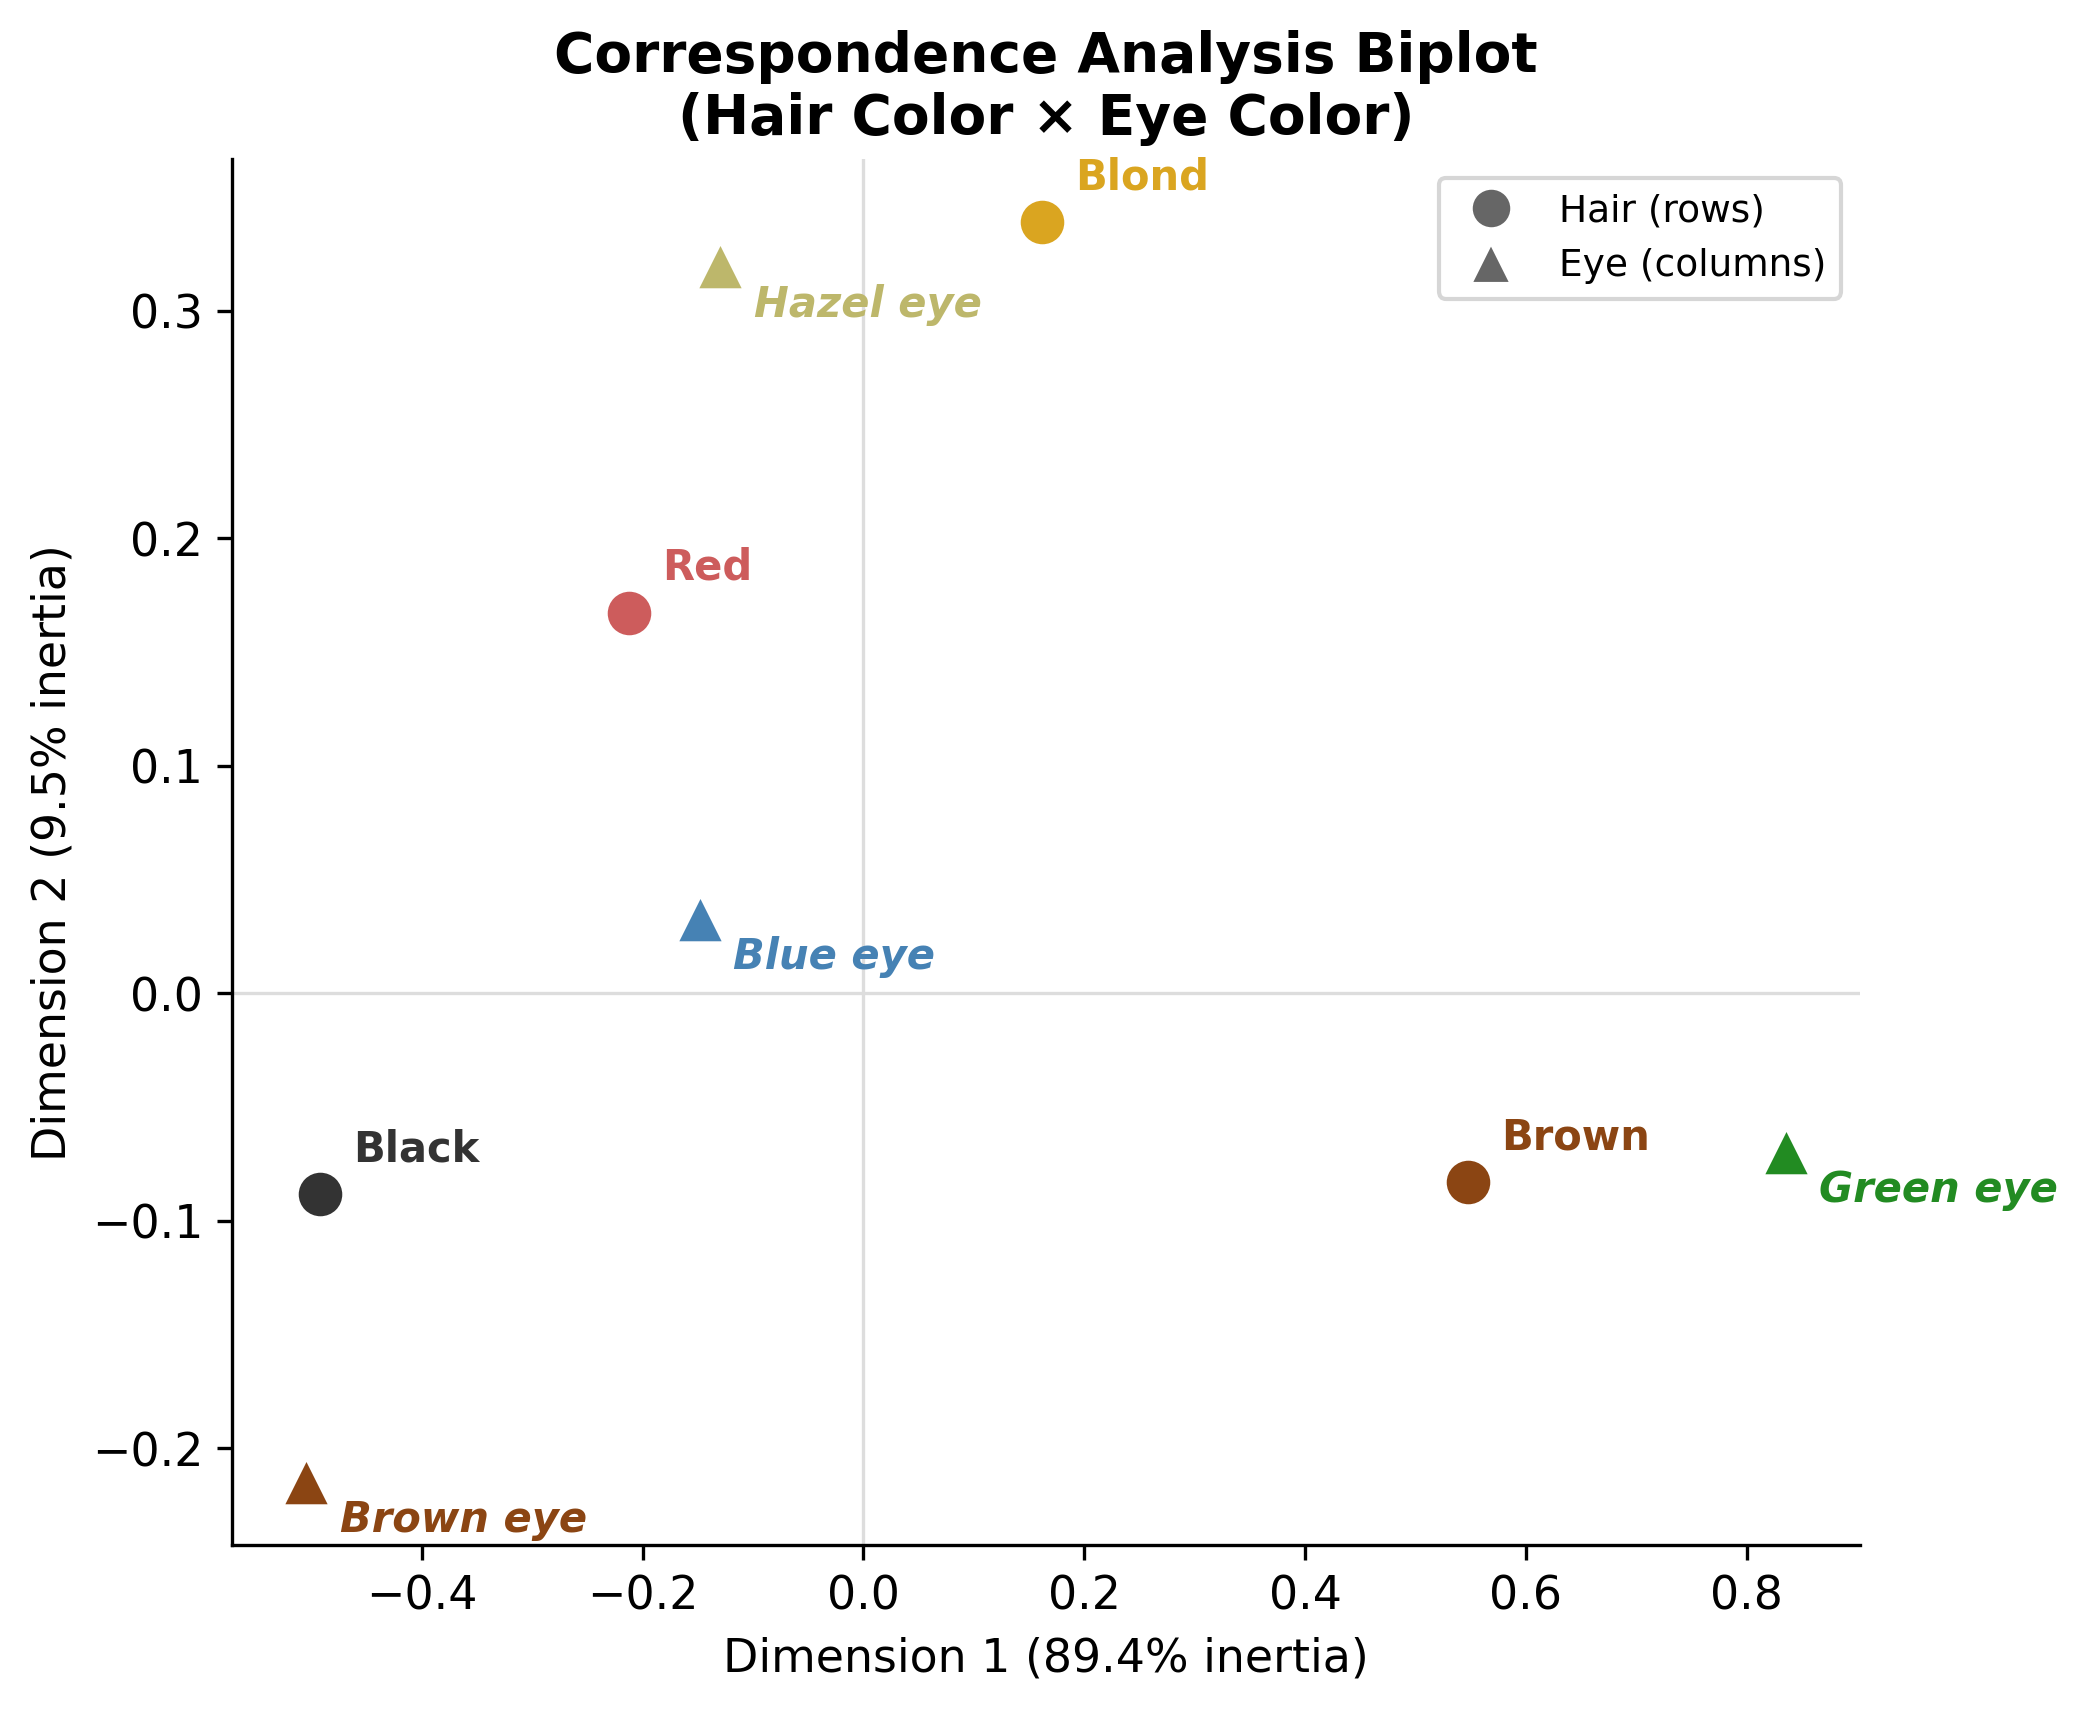
\includegraphics[width=0.62\textwidth]{m3_5_ca_biplot.png}

\vspace{0.2cm}
\begin{columns}[T]
\begin{column}{0.48\textwidth}
\begin{itemize}
    \item Circles = row categories (hair color)
    \item Triangles = column categories (eye color)
    \item Nearby points $\to$ association
    \item Origin = average profile (independence)
    \item Distance from origin = deviation from average
\end{itemize}
\end{column}
\begin{column}{0.48\textwidth}
\begin{exampleblock}{Data Insight}
    \scriptsize Brown hair and Green eye cluster together (right side): brown-haired people are disproportionately green-eyed. Black hair and Brown eye cluster (bottom-left): black hair associates with brown eyes. Dimension 1 captures 89\% of the association.
\end{exampleblock}
\end{column}
\end{columns}
\end{frame}

% ── 127 ──
\begin{frame}{Reading the Biplot: Interpretation Rules}
\smark{127/300}
\begin{columns}[T]
\begin{column}{0.50\textwidth}
\begin{itemize}
    \item \textbf{Row-to-row} distance: similar rows have similar profiles
    \item \textbf{Col-to-col} distance: similar columns have similar profiles
    \item \textbf{Row-to-col} proximity: \emph{approximate} association (in symmetric biplot)
    \item \textbf{Origin}: the average profile (independence)
    \item Points far from origin contribute most to $\chi^2$
\end{itemize}
\end{column}
\begin{column}{0.47\textwidth}
\begin{alertblock}{Pro-Tip}
    \scriptsize In \textbf{symmetric} biplots, row-to-column distances are approximate. In \textbf{asymmetric} biplots (rows in principal, columns in standard, or vice versa), one set's coordinates are exact. Specify which normalization you used.
\end{alertblock}
\vspace{0.1cm}
\begin{exampleblock}{Data Insight}
    \scriptsize The angle from the origin matters: points in the same direction from the origin are positively associated. Points in opposite directions are negatively associated.
\end{exampleblock}
\end{column}
\end{columns}
\end{frame}

% ── 128 ──
\begin{frame}[fragile]{CA Biplot --- \Rlang}\smark{128/300}
\begin{columns}[T]
\begin{column}{0.55\textwidth}
\begin{lstlisting}[style=Rstyle]
library(FactoMineR)
library(factoextra)

# Compute CA
ca_result <- CA(ct, graph=FALSE)

# Biplot (symmetric)
fviz_ca_biplot(ca_result,
  repel = TRUE,
  col.row = "#2166AC",
  col.col = "#B2182B",
  shape.row = 16,
  shape.col = 17) +
  theme_minimal()

# Row points only
fviz_ca_row(ca_result, repel=TRUE)

# Column points only
fviz_ca_col(ca_result, repel=TRUE)
\end{lstlisting}
\end{column}
\begin{column}{0.42\textwidth}
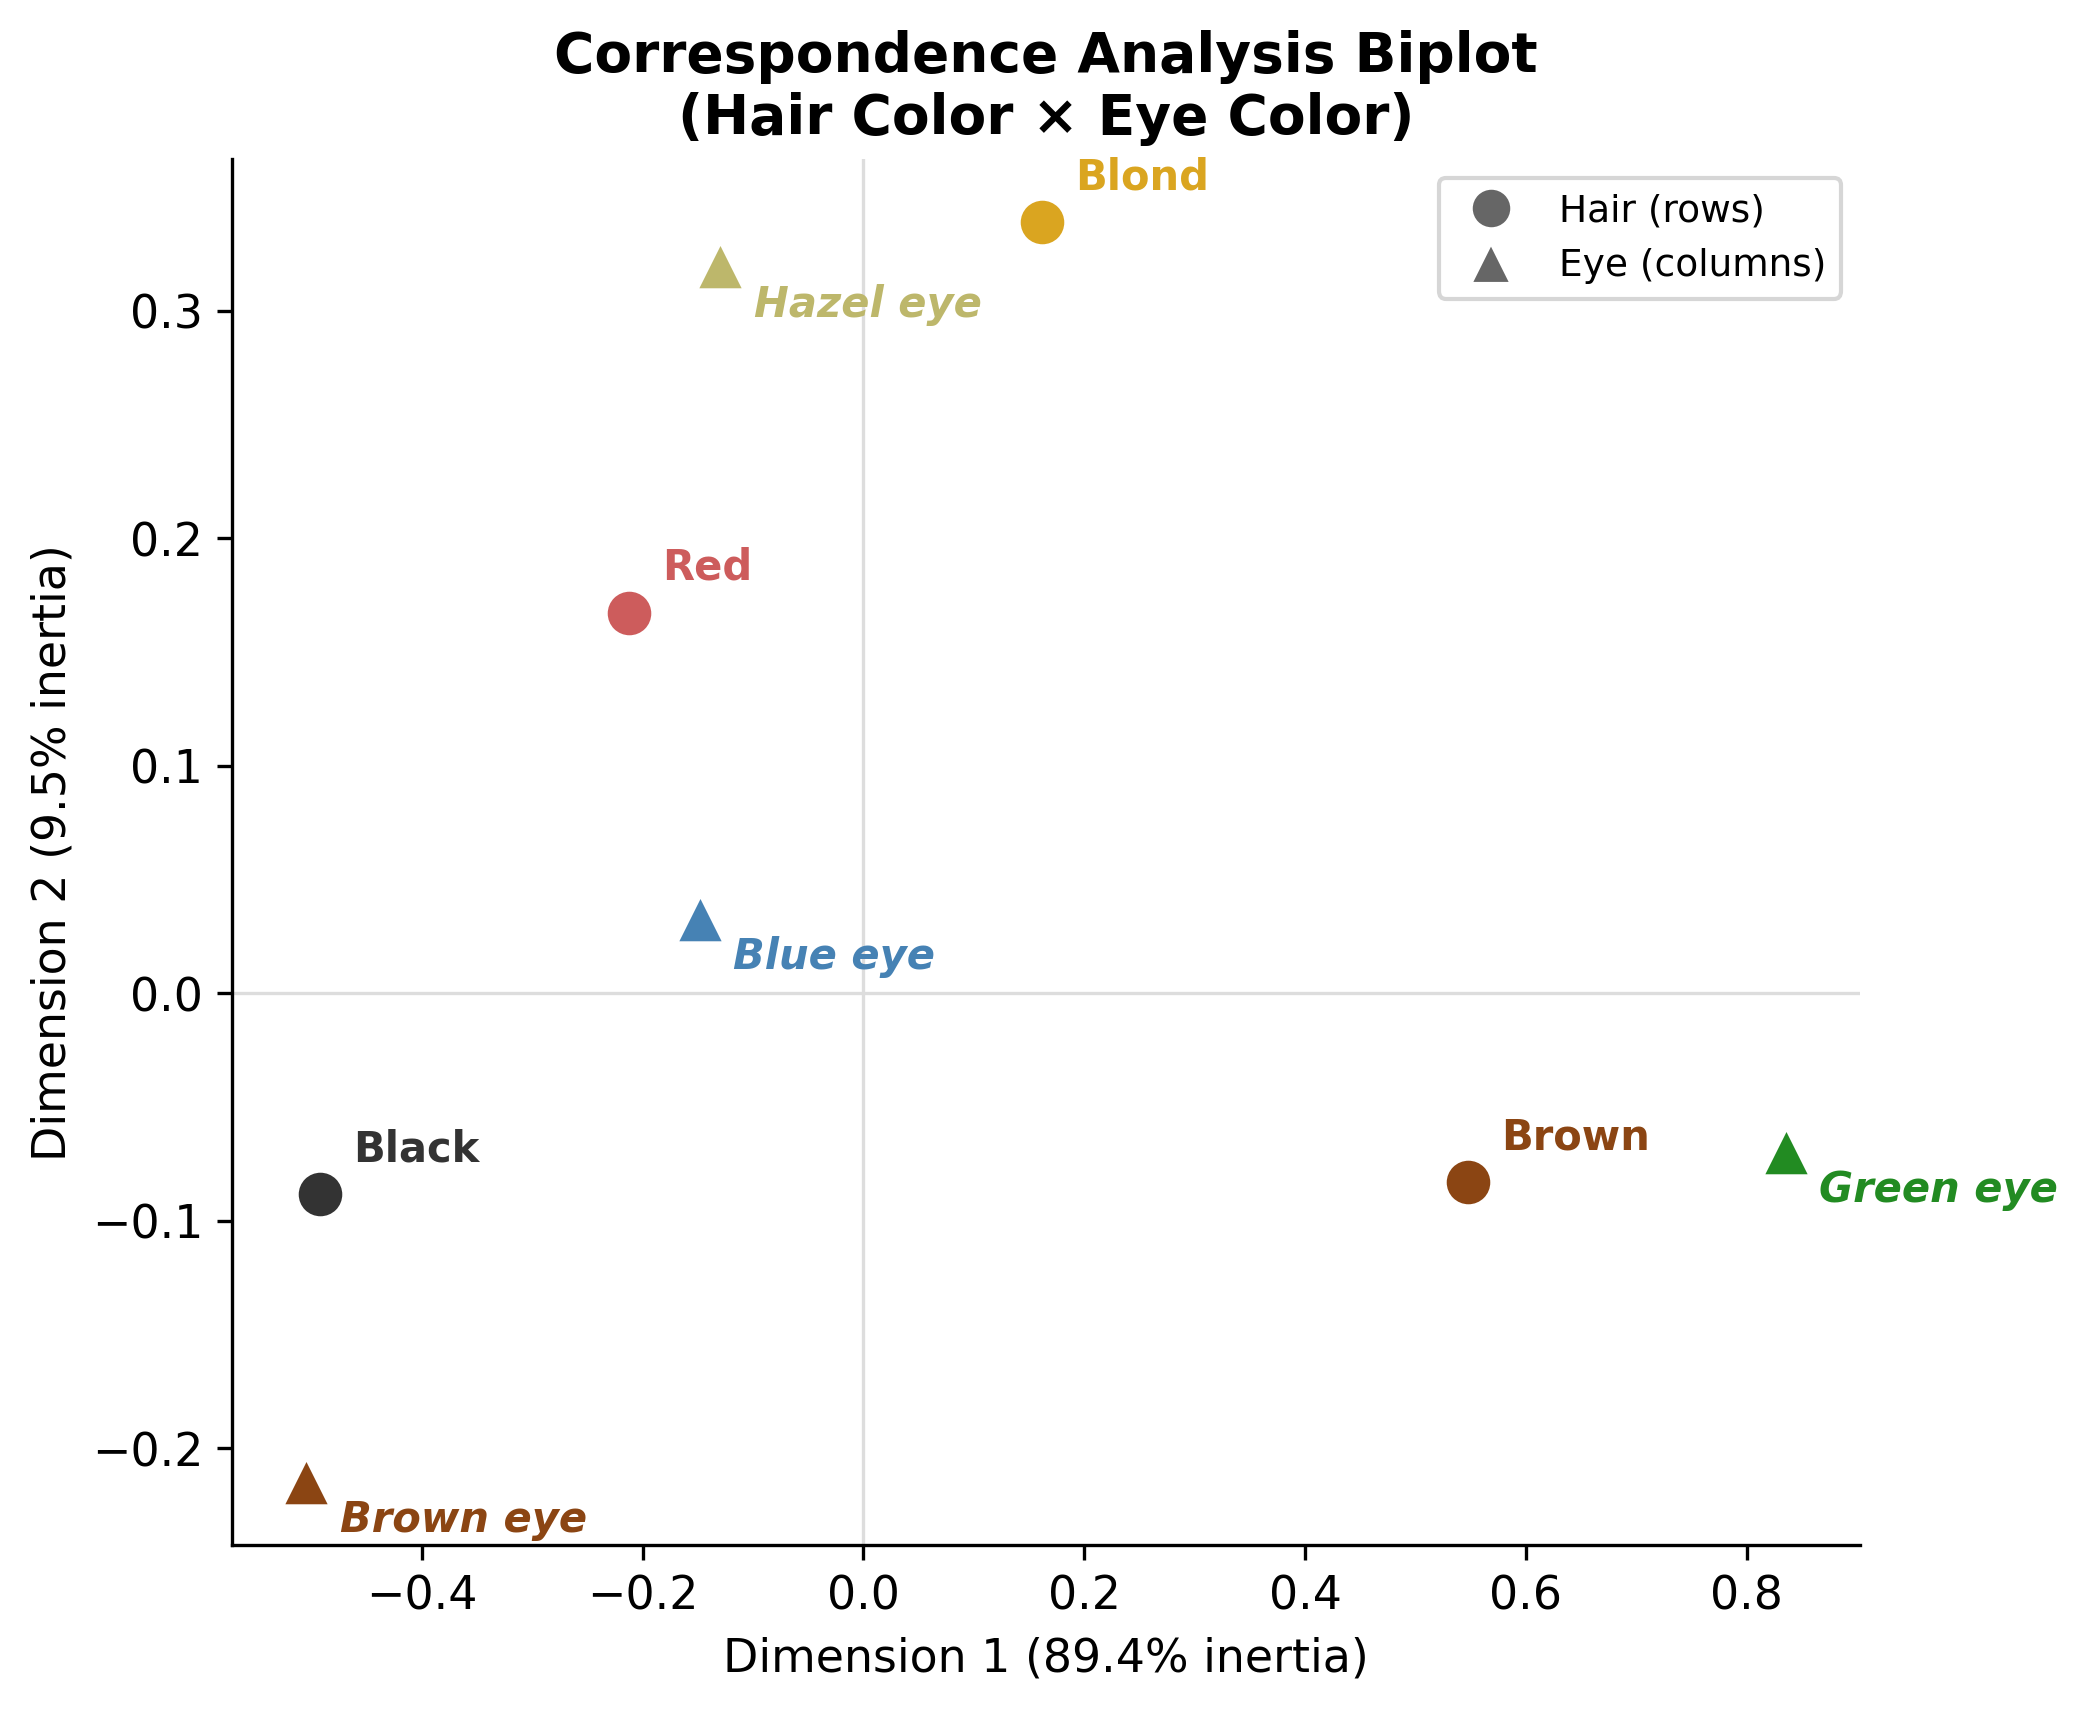
\includegraphics[width=\textwidth]{m3_5_ca_biplot.png}
\begin{alertblock}{Pro-Tip}
    \scriptsize \texttt{FactoMineR::CA()} computes the analysis; \texttt{factoextra::fviz\_ca\_biplot()} produces the ggplot2-based display. \texttt{repel=TRUE} avoids label overlap (uses ggrepel internally).
\end{alertblock}
\end{column}
\end{columns}
\end{frame}

% ── 129 ──
\begin{frame}[fragile]{CA Biplot --- \Python}\smark{129/300}
\begin{columns}[T]
\begin{column}{0.55\textwidth}
\begin{lstlisting}[style=Pystyle]
# prince (CA library)
import prince

ca = prince.CA(n_components=2)
ca = ca.fit(ct_df)

# Biplot
ax = ca.plot(ct_df,
    x_component=0,
    y_component=1)

# Manual from coordinates
row_coords = ca.row_coordinates(ct_df)
col_coords = ca.column_coordinates(
    ct_df)

ax.scatter(row_coords[0],
    row_coords[1], marker="o",
    label="Rows")
ax.scatter(col_coords[0],
    col_coords[1], marker="^",
    label="Columns")

# Inertia
print(ca.percentage_of_variance_)
\end{lstlisting}
\end{column}
\begin{column}{0.42\textwidth}
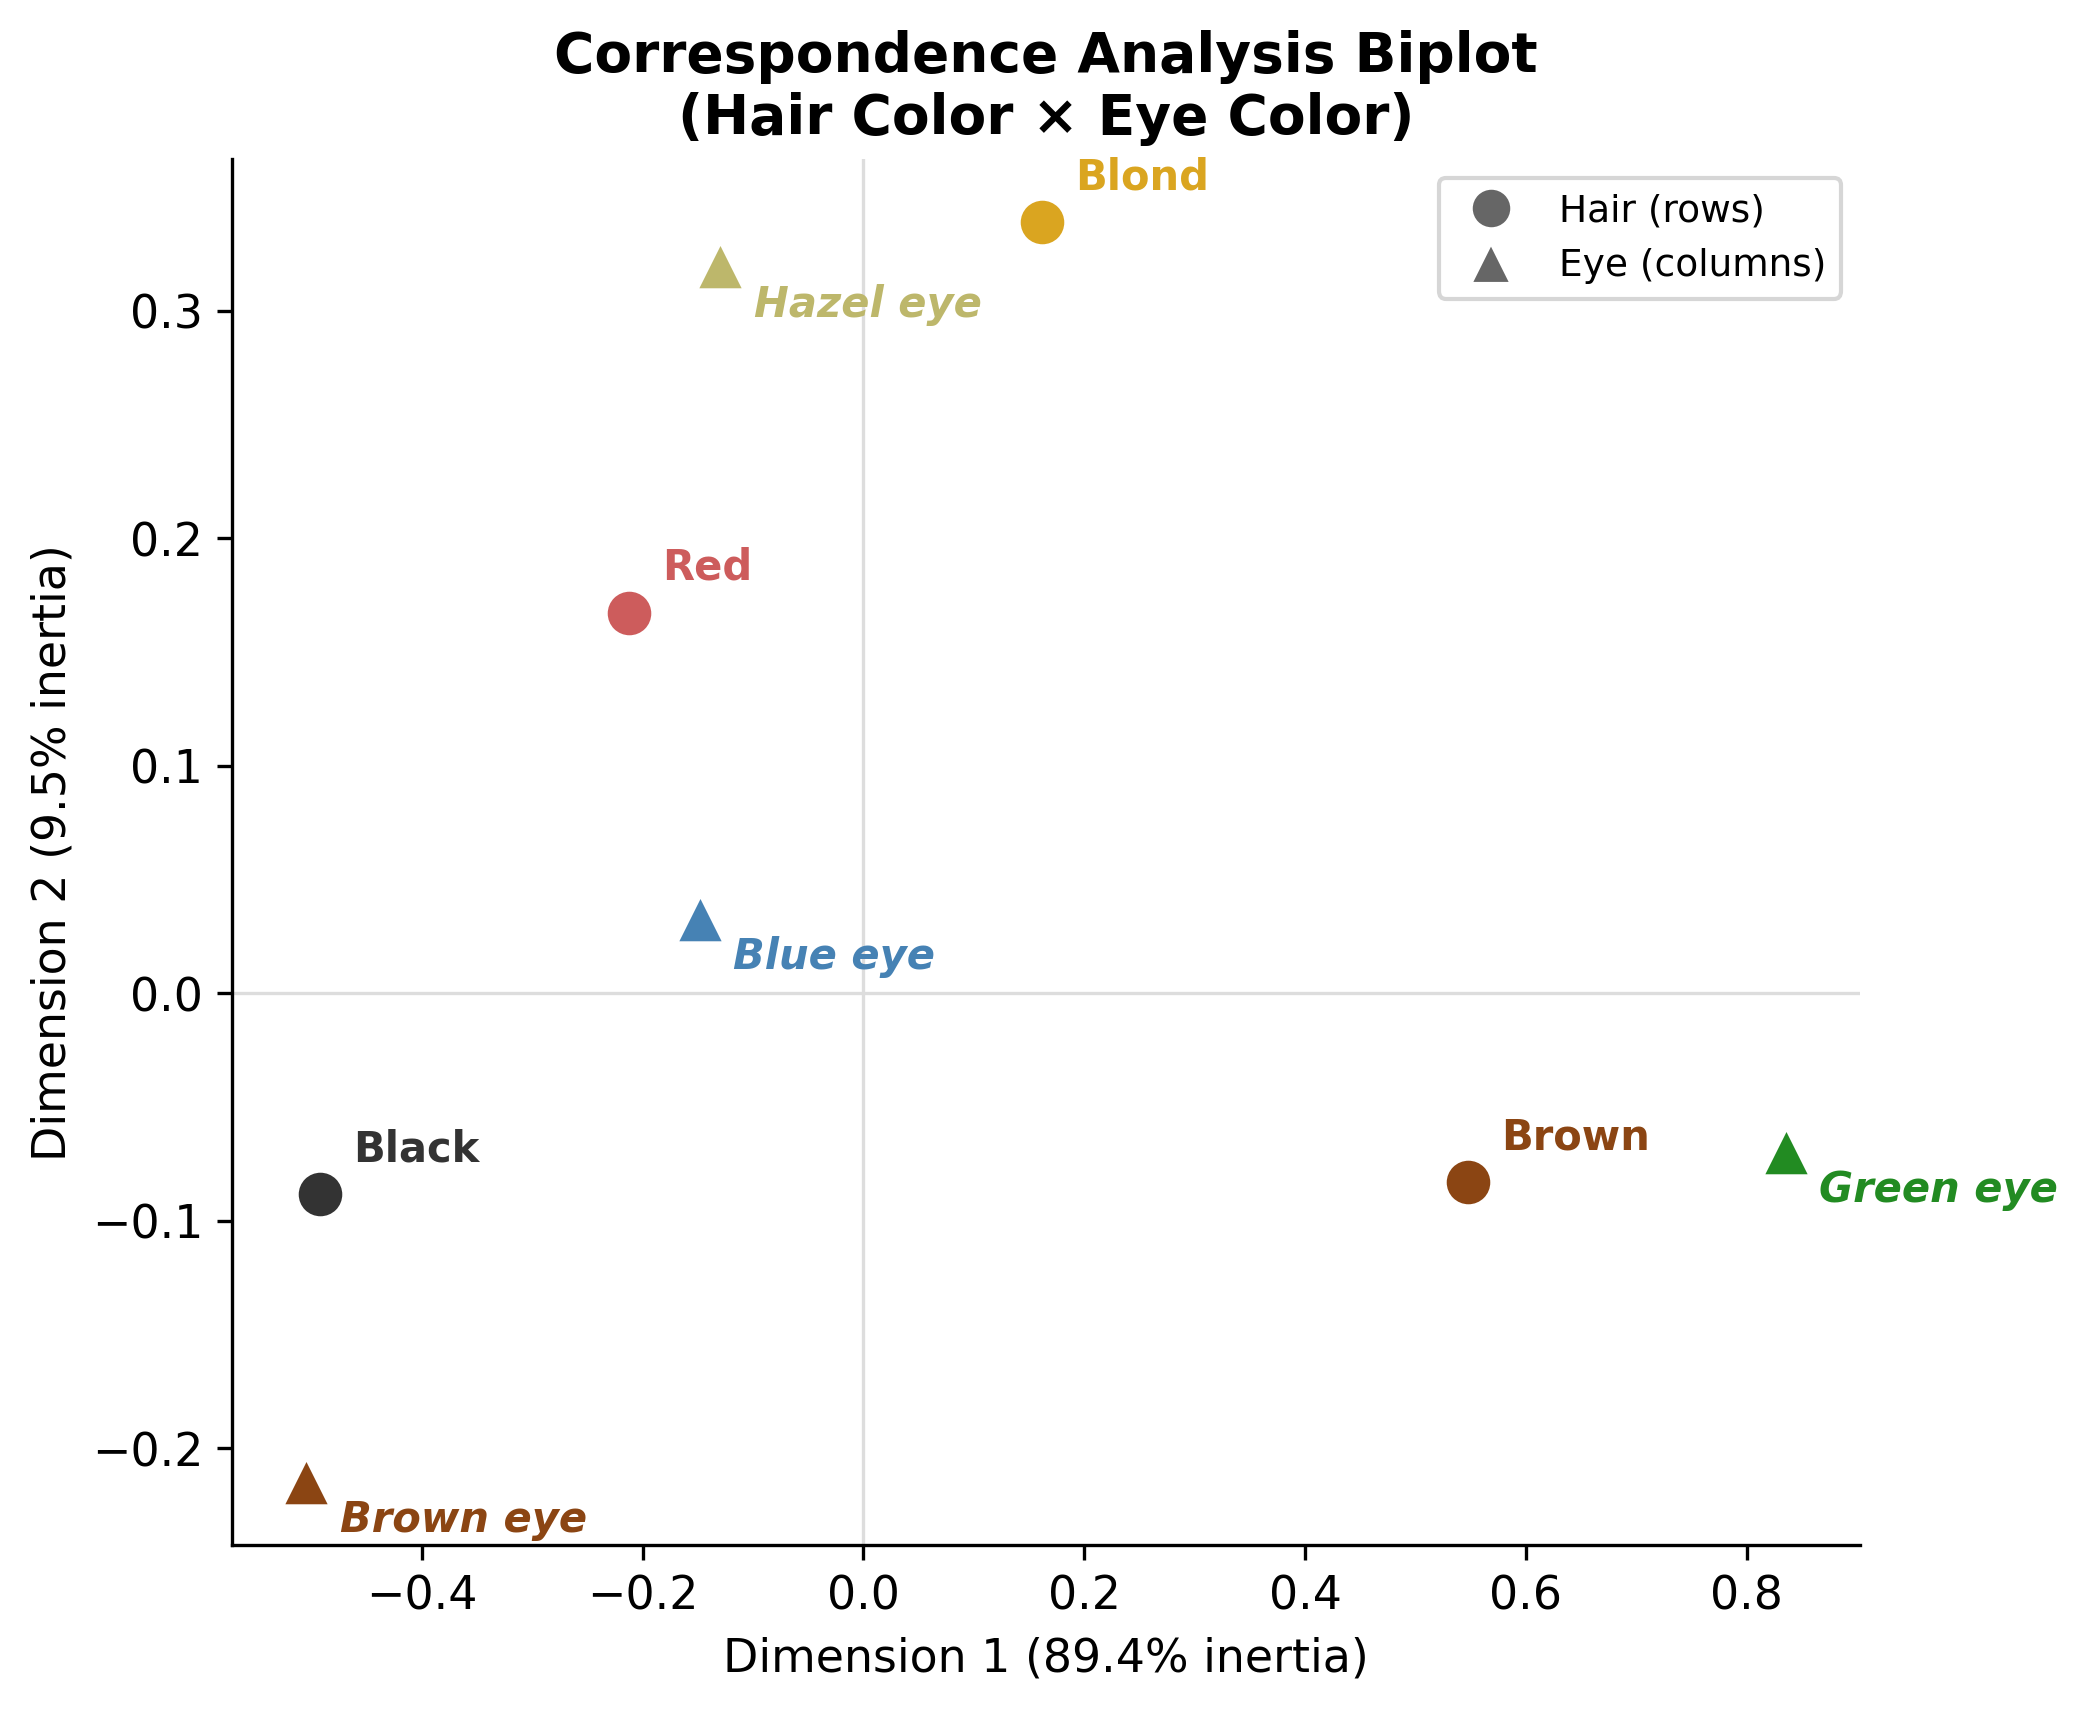
\includegraphics[width=\textwidth]{m3_5_ca_biplot.png}
\begin{exampleblock}{Data Insight}
    \scriptsize The \texttt{prince} Python package provides CA, MCA, and related methods with a scikit-learn-compatible API. \texttt{ca.plot()} produces a basic biplot; extract coordinates for custom matplotlib plots.
\end{exampleblock}
\end{column}
\end{columns}
\end{frame}

% ── 130 ──
\begin{frame}{Inertia: The CA Equivalent of Variance}
\smark{130/300}
\centering
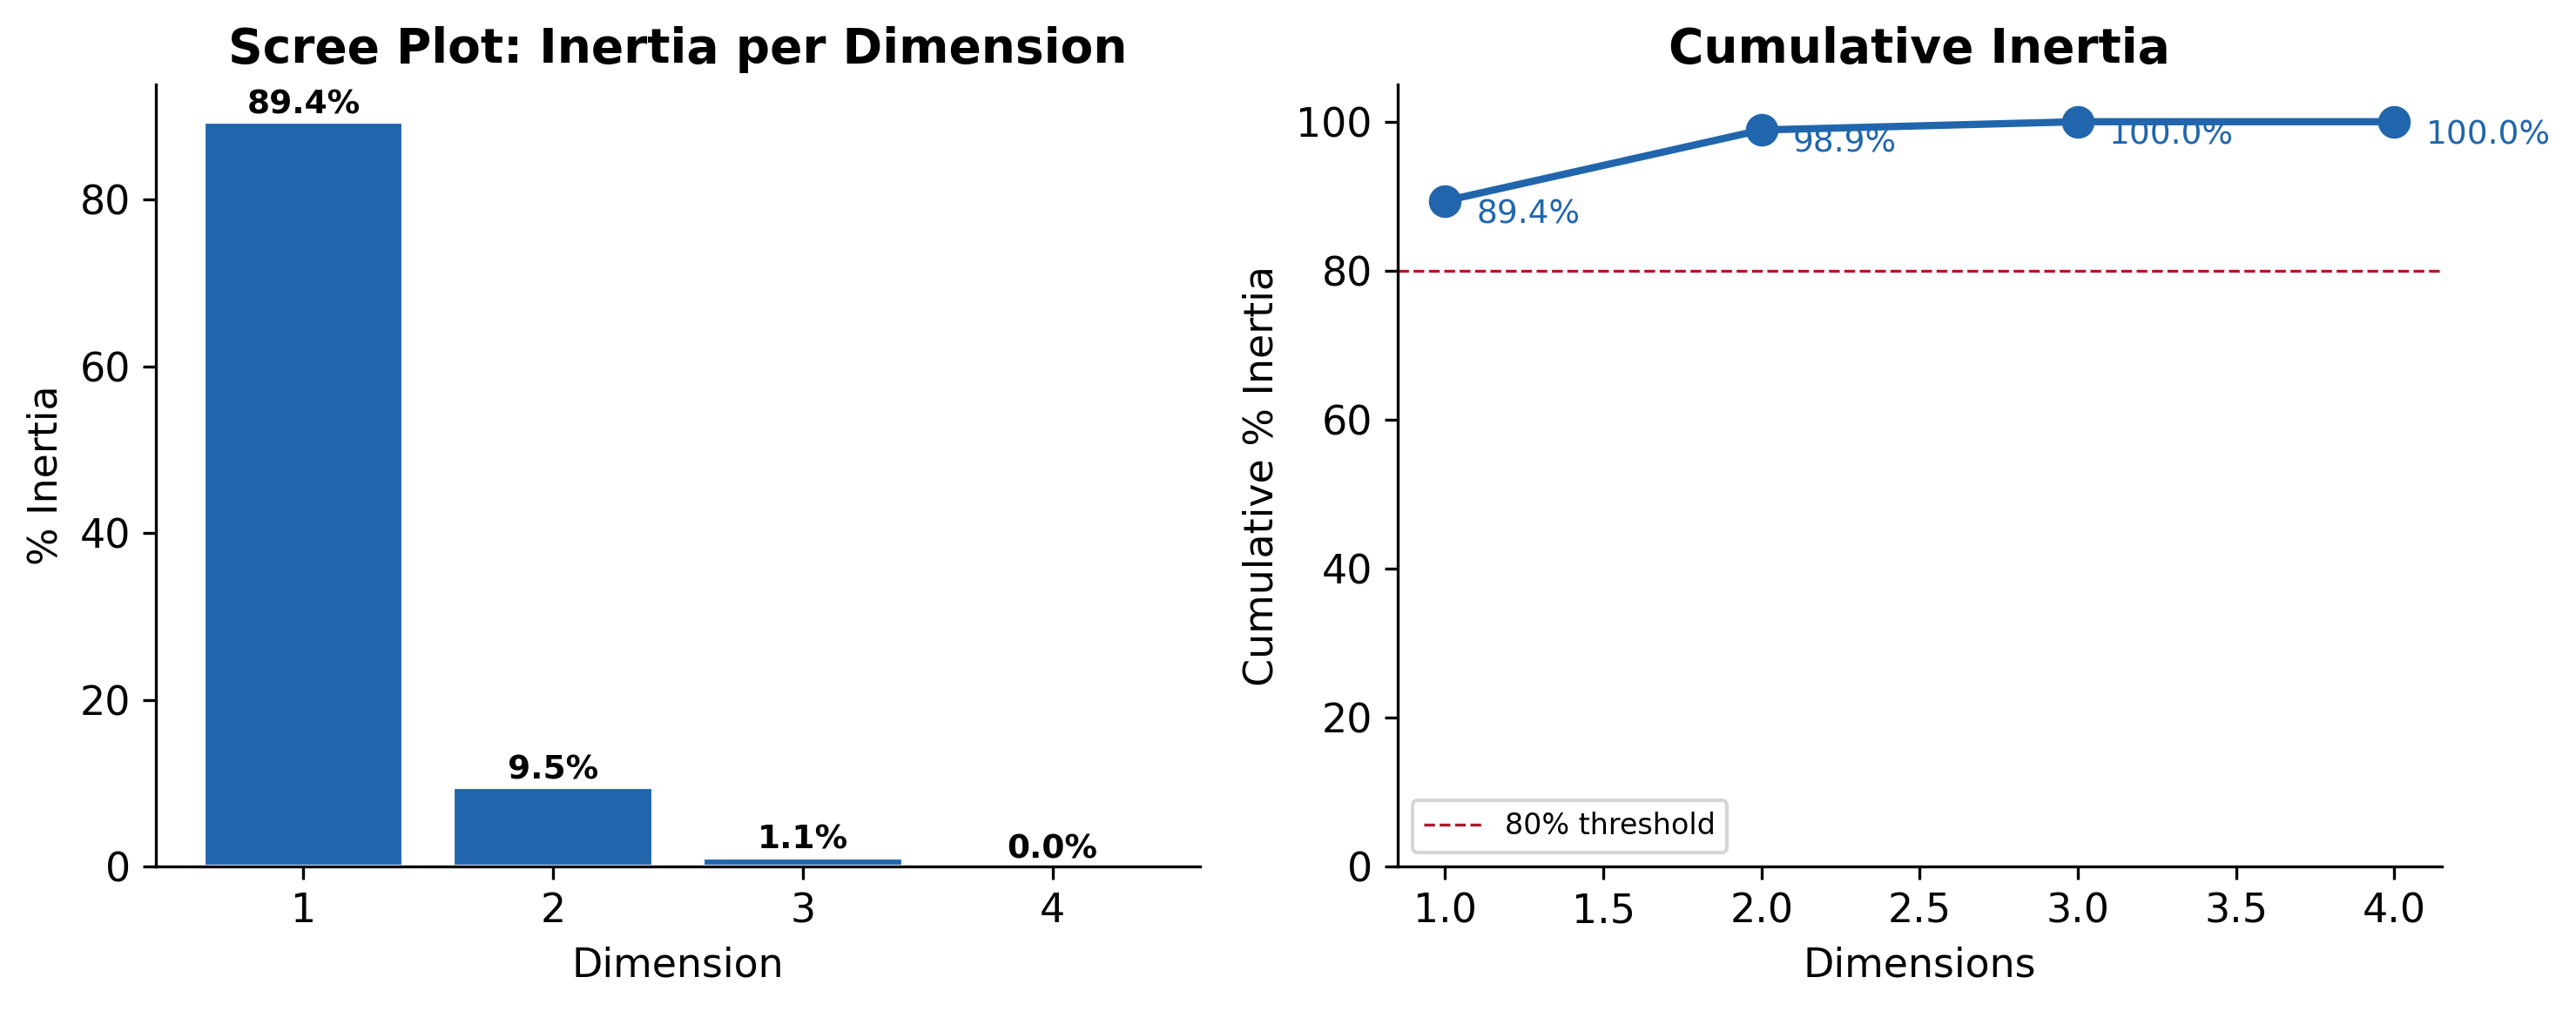
\includegraphics[width=0.88\textwidth]{m3_5_scree.png}

\vspace{0.2cm}
\begin{columns}[T]
\begin{column}{0.48\textwidth}
\begin{itemize}
    \item \textbf{Total inertia} = $\chi^2 / N$ (normalized $\chi^2$)
    \item Each dimension captures a fraction of total inertia
    \item Scree plot: analogous to PCA eigenvalue plot
    \item Keep dimensions until cumulative inertia $> 80$\%
\end{itemize}
\end{column}
\begin{column}{0.48\textwidth}
\begin{exampleblock}{Data Insight}
    \scriptsize Dimension 1 captures 89.4\% of the inertia --- the association is essentially one-dimensional. This is common for $2 \times k$ or small tables. For larger tables, 2--3 dimensions may be needed.
\end{exampleblock}
\end{column}
\end{columns}
\end{frame}

% ── 131 ──
\begin{frame}[fragile]{Scree Plot --- Code}\smark{131/300}
\begin{columns}[T]
\begin{column}{0.48\textwidth}
\begin{lstlisting}[style=Rstyle]
library(factoextra)

# Scree plot
fviz_screeplot(ca_result,
  addlabels = TRUE,
  barfill = "#2166AC",
  linecolor = "#B2182B") +
  theme_minimal()

# Numeric summary
summary(ca_result)
# Shows eigenvalues, % variance,
# cumulative %
\end{lstlisting}
\end{column}
\begin{column}{0.48\textwidth}
\begin{lstlisting}[style=Pystyle]
# prince
inertia = ca.percentage_of_variance_

fig, ax = plt.subplots()
ax.bar(range(1, len(inertia)+1),
    inertia, color="#2166AC")
ax.set_xlabel("Dimension")
ax.set_ylabel("% Inertia")
ax.set_title("Scree Plot")

# Cumulative
cum = np.cumsum(inertia)
ax2 = ax.twinx()
ax2.plot(range(1, len(inertia)+1),
    cum, "o-", color="#B2182B")
ax2.axhline(80, linestyle="--")
\end{lstlisting}
\end{column}
\end{columns}
\end{frame}

% ── 132 ──
\begin{frame}{Contributions: Which Categories Drive Each Dimension?}
\smark{132/300}
\centering
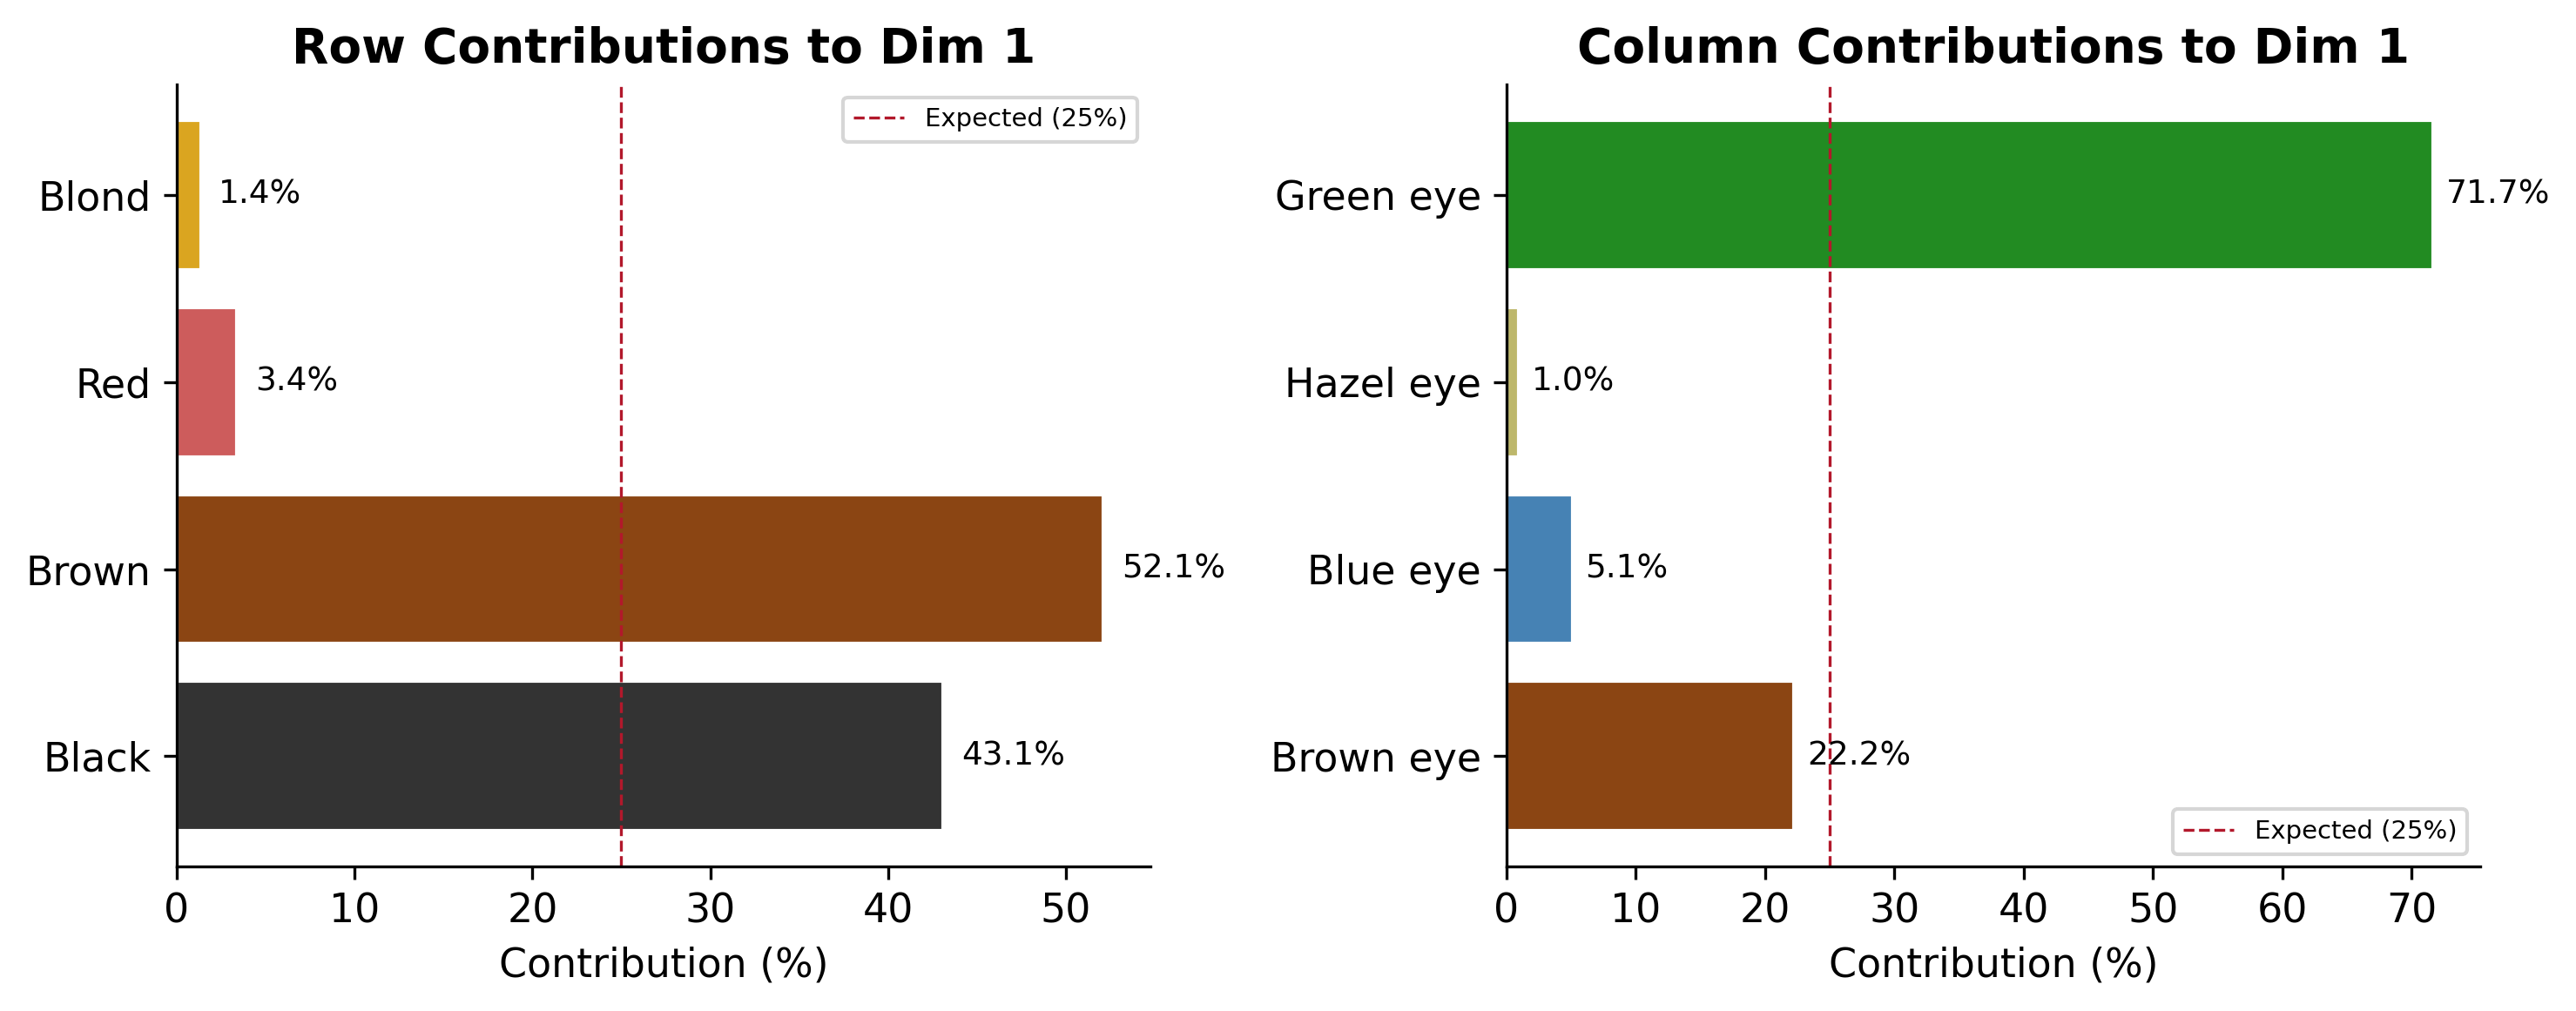
\includegraphics[width=0.88\textwidth]{m3_5_contributions.png}

\vspace{0.2cm}
\begin{columns}[T]
\begin{column}{0.48\textwidth}
\begin{itemize}
    \item Contribution = how much a point contributes to the dimension's inertia
    \item If $k$ categories: expected contribution = $1/k$ (uniform)
    \item Points above $1/k$ are ``important'' for that dimension
    \item Dashed red line = expected contribution under uniformity
\end{itemize}
\end{column}
\begin{column}{0.48\textwidth}
\begin{alertblock}{Pro-Tip}
    \scriptsize R: \texttt{fviz\_contrib(ca\_result, choice="row", axes=1)} produces the contribution bar chart. Filter to show only points above the expected threshold: these are the categories that \emph{define} each dimension.
\end{alertblock}
\end{column}
\end{columns}
\end{frame}

% ── 133 ──
\begin{frame}[fragile]{Contributions --- Code}\smark{133/300}
\begin{columns}[T]
\begin{column}{0.48\textwidth}
\begin{lstlisting}[style=Rstyle]
# Row contributions to Dim 1
fviz_contrib(ca_result,
  choice = "row",
  axes = 1,
  fill = "#2166AC") +
  theme_minimal()

# Column contributions to Dim 2
fviz_contrib(ca_result,
  choice = "col",
  axes = 2,
  fill = "#B2182B")

# Numeric
ca_result$row$contrib  # matrix
ca_result$col$contrib
\end{lstlisting}
\end{column}
\begin{column}{0.48\textwidth}
\begin{lstlisting}[style=Pystyle]
# prince
row_contrib = ca.row_contributions_
col_contrib = ca.column_contributions_

# Bar chart for Dim 1
ax.barh(row_labels,
    row_contrib.iloc[:, 0] * 100,
    color="#2166AC")
ax.axvline(100/len(row_labels),
    linestyle="--", color="#B2182B",
    label="Expected")
ax.set_xlabel("Contribution (%)")
ax.legend()

# Manual computation
# contrib_i = mass_i * coord_i^2
#             / eigenvalue_k
\end{lstlisting}
\end{column}
\end{columns}
\end{frame}

% ── 134 ──
\begin{frame}{Quality of Representation: cos$^2$}
\smark{134/300}
\centering
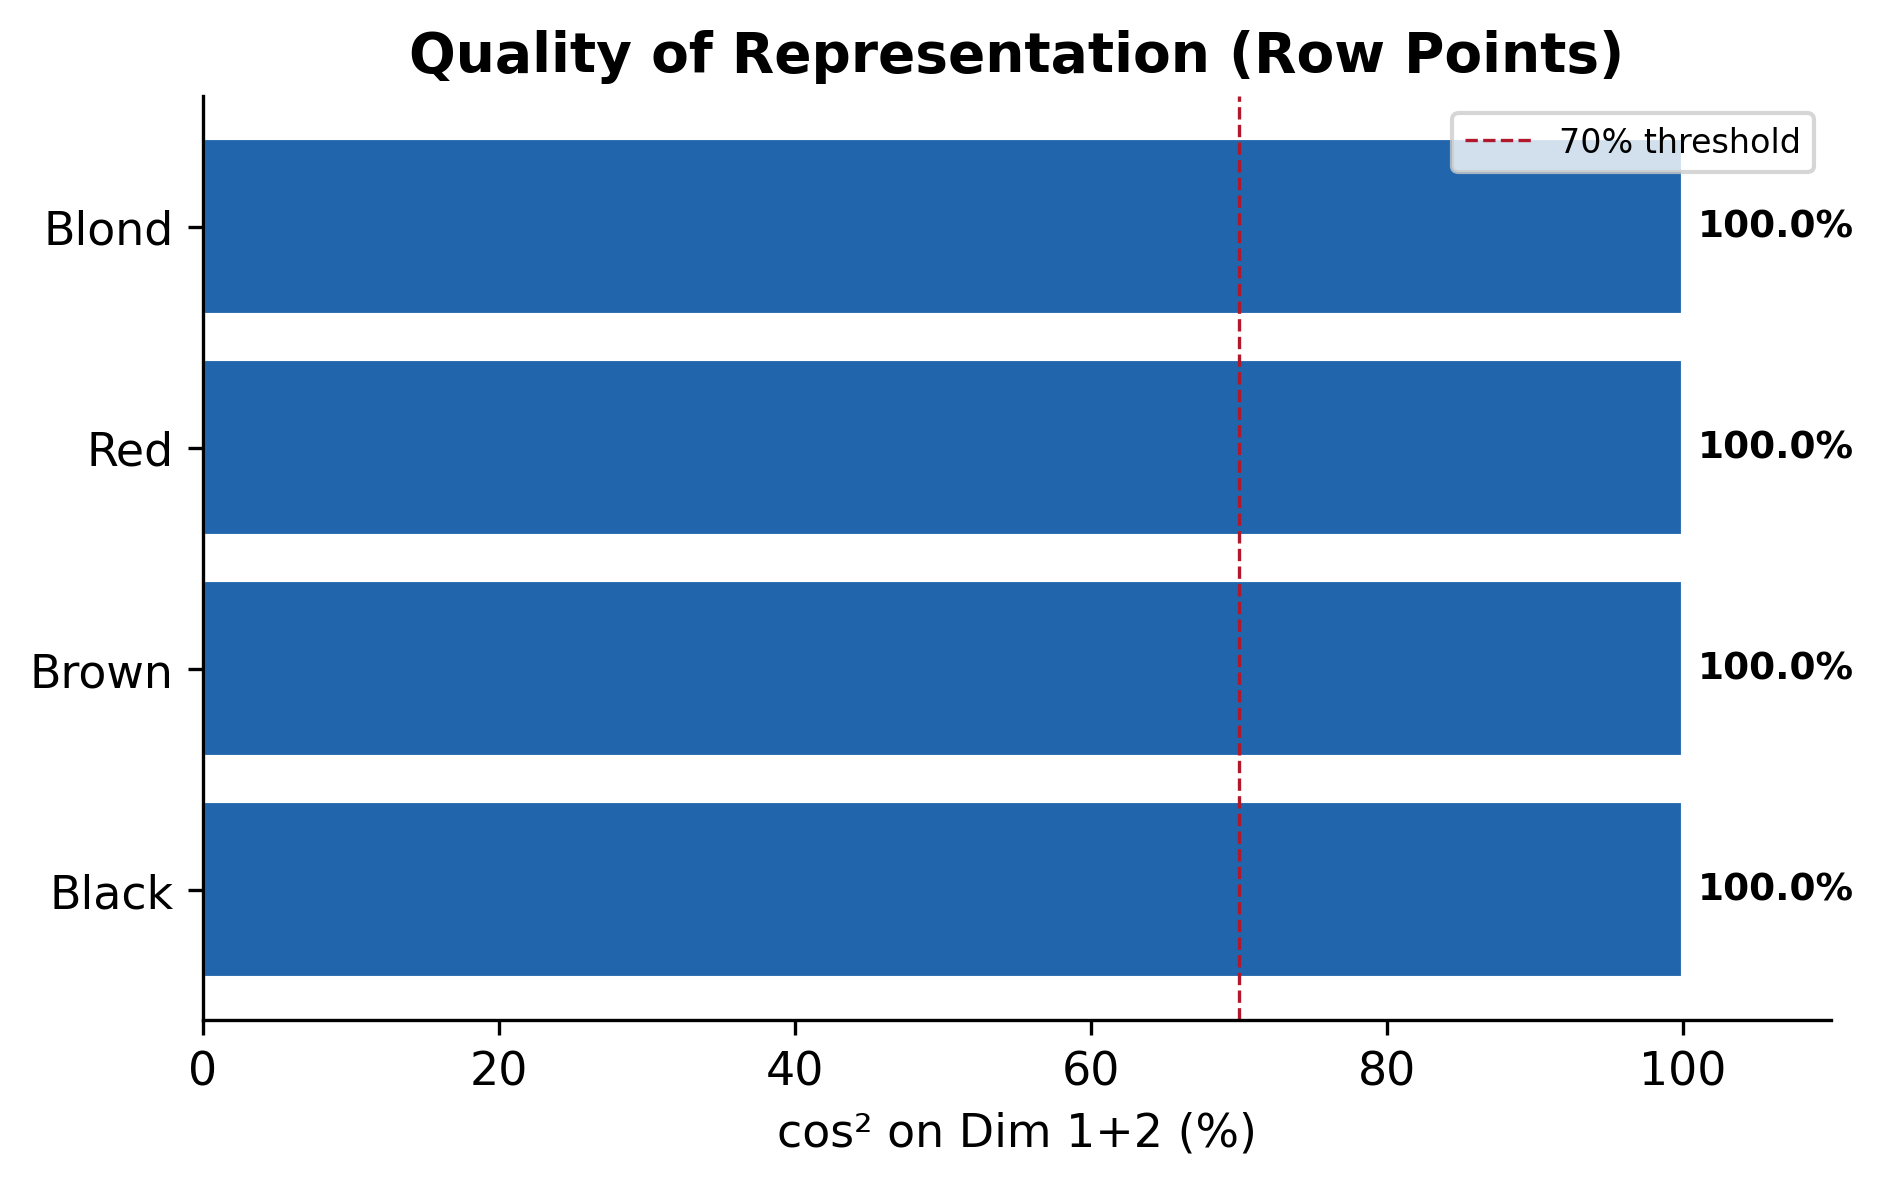
\includegraphics[width=0.62\textwidth]{m3_5_cos2.png}

\vspace{0.2cm}
\begin{columns}[T]
\begin{column}{0.48\textwidth}
\begin{itemize}
    \item $\cos^2$ = proportion of a point's inertia captured in the displayed dimensions
    \item High $\cos^2$ ($> 0.7$): point is well-represented on the biplot
    \item Low $\cos^2$ ($< 0.3$): point's position is misleading --- it needs more dimensions
    \item Color or size points by $\cos^2$ on the biplot
\end{itemize}
\end{column}
\begin{column}{0.48\textwidth}
\begin{alertblock}{Pro-Tip}
    \scriptsize R: \texttt{fviz\_ca\_biplot(ca\_result, col.row="cos2")} colors points by quality of representation. Poorly represented points should be \emph{greyed out} or flagged with a warning.
\end{alertblock}
\end{column}
\end{columns}
\end{frame}

% ── 135 ──
\begin{frame}[fragile]{cos$^2$ --- Code}\smark{135/300}
\begin{columns}[T]
\begin{column}{0.48\textwidth}
\begin{lstlisting}[style=Rstyle]
# Color by cos2 (quality)
fviz_ca_biplot(ca_result,
  col.row = "cos2",
  col.col = "cos2",
  gradient.cols = c("#EEEEEE",
    "#2166AC", "#B2182B"),
  repel = TRUE)

# Numeric
ca_result$row$cos2
ca_result$col$cos2

# Bar chart of cos2
fviz_cos2(ca_result,
  choice = "row", axes = 1:2)
\end{lstlisting}
\end{column}
\begin{column}{0.48\textwidth}
\begin{lstlisting}[style=Pystyle]
# prince
row_cos2 = ca.row_cosine_similarities(
    ct_df)
col_cos2 = ca.column_cosine_similarities(
    ct_df)

# Color points by cos2
cos2_dim12 = row_cos2.iloc[:,:2]\
    .sum(axis=1)
sc = ax.scatter(coords[:,0],
    coords[:,1],
    c=cos2_dim12,
    cmap="RdYlBu_r", vmin=0, vmax=1)
plt.colorbar(sc, label="cos²")
\end{lstlisting}
\vspace{0.1cm}
\begin{exampleblock}{Data Insight}
    \scriptsize $\cos^2$ is the CA analog of ``communality'' in factor analysis. It tells you whether a point's biplot position is trustworthy.
\end{exampleblock}
\end{column}
\end{columns}
\end{frame}

% ── 136 ──
\begin{frame}{Multiple Correspondence Analysis (MCA)}
\smark{136/300}
\centering
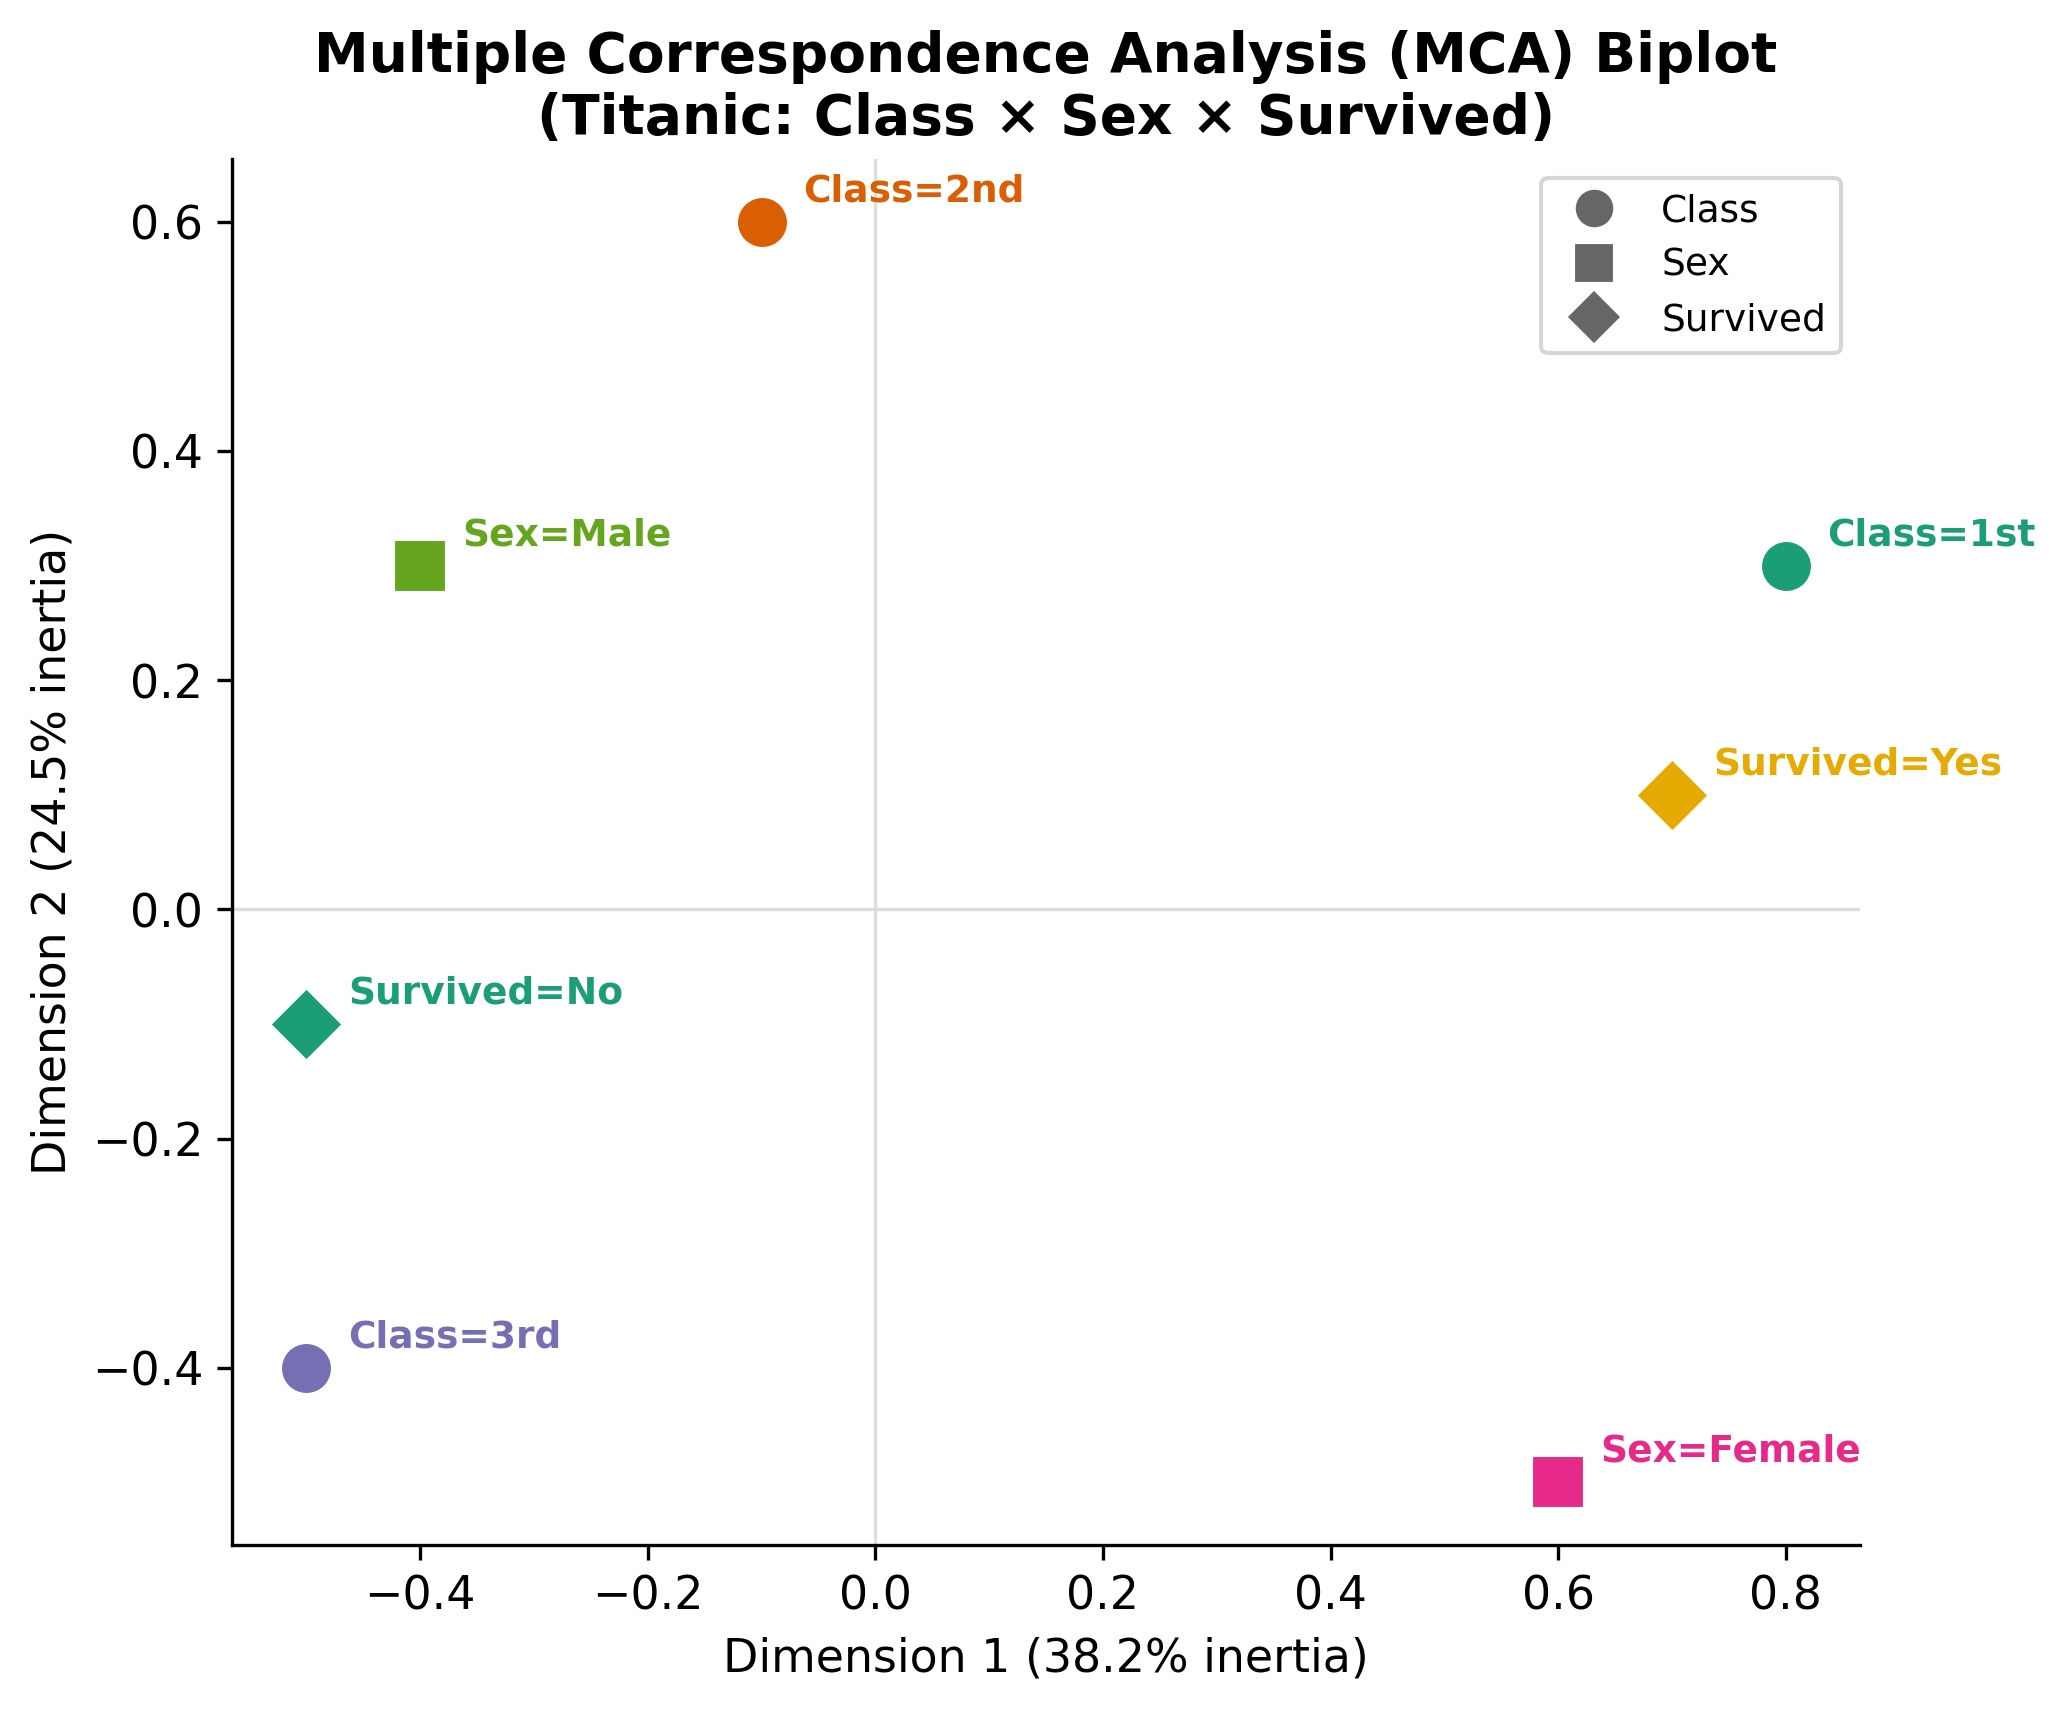
\includegraphics[width=0.62\textwidth]{m3_5_mca_biplot.png}

\vspace{0.2cm}
\begin{columns}[T]
\begin{column}{0.48\textwidth}
\begin{itemize}
    \item CA for $> 2$ categorical variables
    \item Input: indicator (dummy) matrix or Burt matrix
    \item Projects all category levels into a shared space
    \item Reveals which levels of different variables \textbf{co-occur}
    \item Common in social science, marketing, ecology
\end{itemize}
\end{column}
\begin{column}{0.48\textwidth}
\begin{exampleblock}{Data Insight}
    \scriptsize 1st class, Female, and Survived cluster together (upper-right): the ``women and children first'' pattern. 3rd class, Male, and No cluster (lower-left): the at-risk group. MCA reveals multi-variable patterns that mosaic plots handle only pairwise.
\end{exampleblock}
\end{column}
\end{columns}
\end{frame}

% ── 137 ──
\begin{frame}[fragile]{MCA --- \Rlang}\smark{137/300}
\begin{columns}[T]
\begin{column}{0.55\textwidth}
\begin{lstlisting}[style=Rstyle]
library(FactoMineR)
library(factoextra)

# All variables must be factors
titanic_cat <- titanic |>
  select(class, sex, survived) |>
  mutate(across(everything(),
    as.factor))

# Compute MCA
mca_result <- MCA(titanic_cat,
  graph = FALSE)

# Biplot of variable categories
fviz_mca_var(mca_result,
  repel = TRUE,
  col.var = "contrib",
  gradient.cols = c("#EEEEEE",
    "#2166AC", "#B2182B")) +
  theme_minimal()

# Individual factor map
fviz_mca_ind(mca_result,
  habillage = "survived",
  palette = c("#B2182B","#1B9E77"))
\end{lstlisting}
\end{column}
\begin{column}{0.42\textwidth}
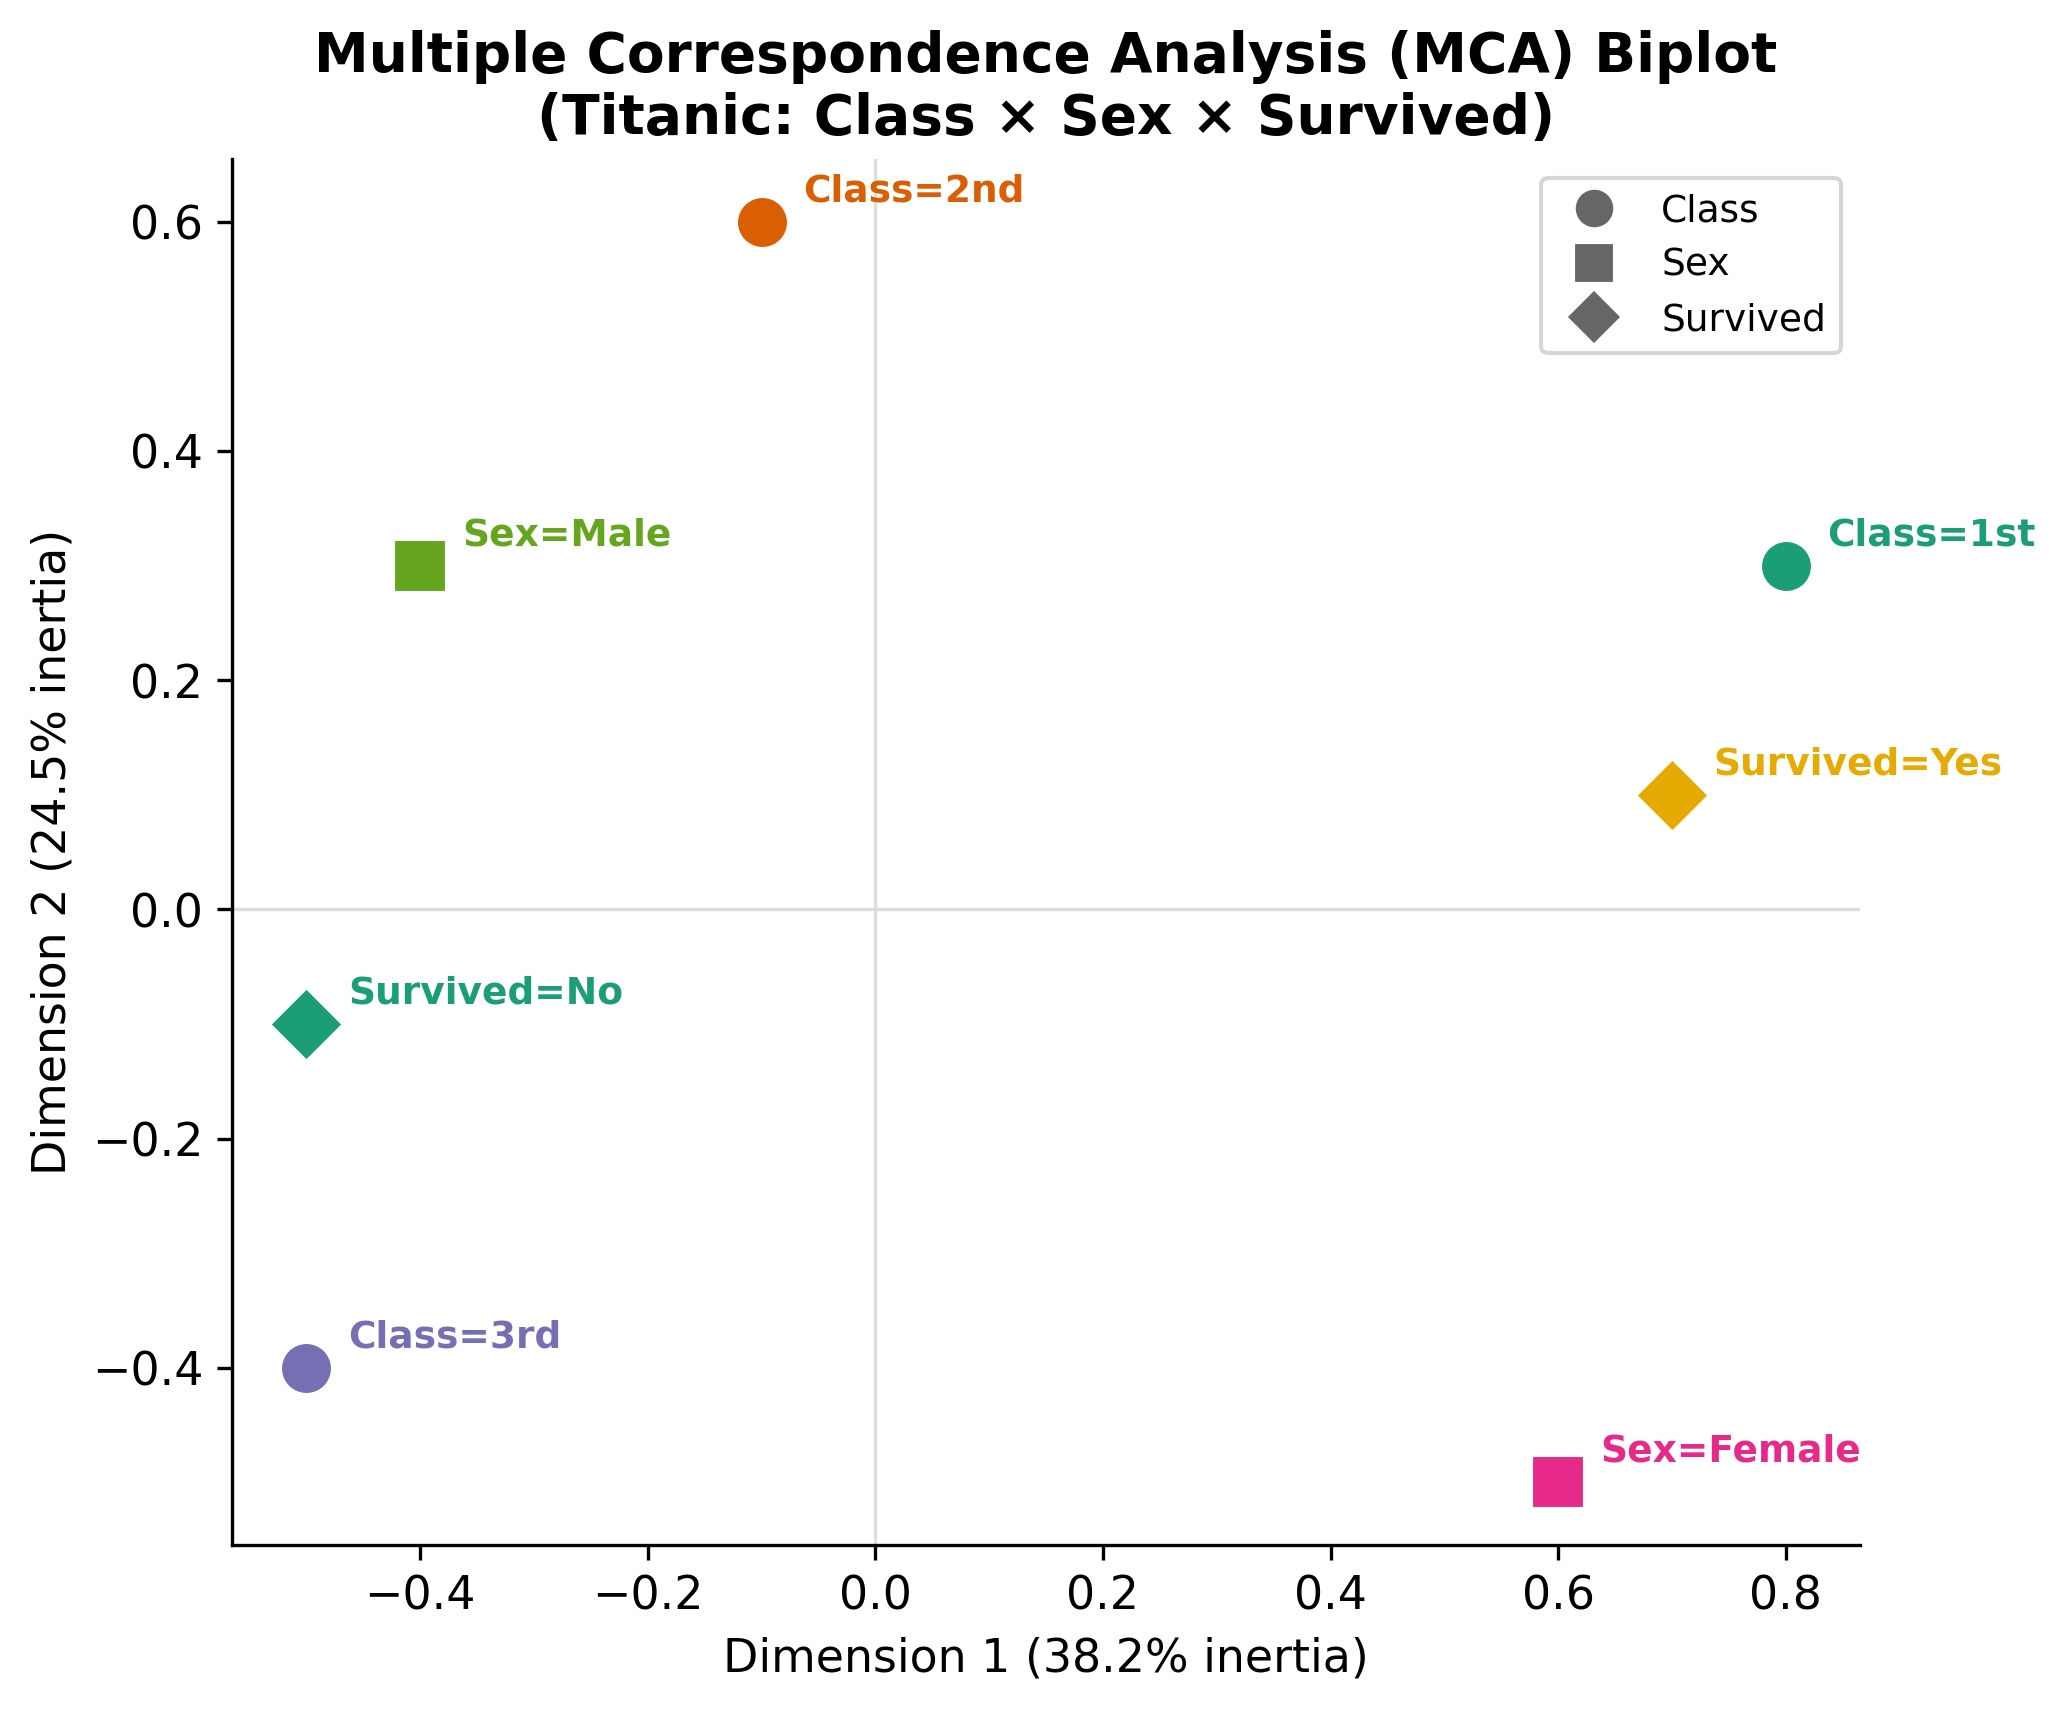
\includegraphics[width=\textwidth]{m3_5_mca_biplot.png}
\begin{alertblock}{Pro-Tip}
    \scriptsize \texttt{fviz\_mca\_var()} shows category-level points (what we interpret). \texttt{fviz\_mca\_ind()} shows individual observations (useful for clustering). Both are part of the \texttt{factoextra} toolkit.
\end{alertblock}
\end{column}
\end{columns}
\end{frame}

% ── 138 ──
\begin{frame}[fragile]{MCA --- \Python}\smark{138/300}
\begin{columns}[T]
\begin{column}{0.55\textwidth}
\begin{lstlisting}[style=Pystyle]
import prince

mca = prince.MCA(n_components=2)
mca = mca.fit(titanic[
    ["class","sex","survived"]])

# Variable category coordinates
coords = mca.column_coordinates(
    titanic[["class","sex",
             "survived"]])

# Biplot
ax = mca.plot(titanic[
    ["class","sex","survived"]],
    x_component=0,
    y_component=1)

# Manual: custom markers per variable
for var in ["class","sex","survived"]:
    sub = coords.loc[
        coords.index.str.startswith(
            var)]
    ax.scatter(sub[0], sub[1],
        marker=markers[var], s=100)
\end{lstlisting}
\end{column}
\begin{column}{0.42\textwidth}
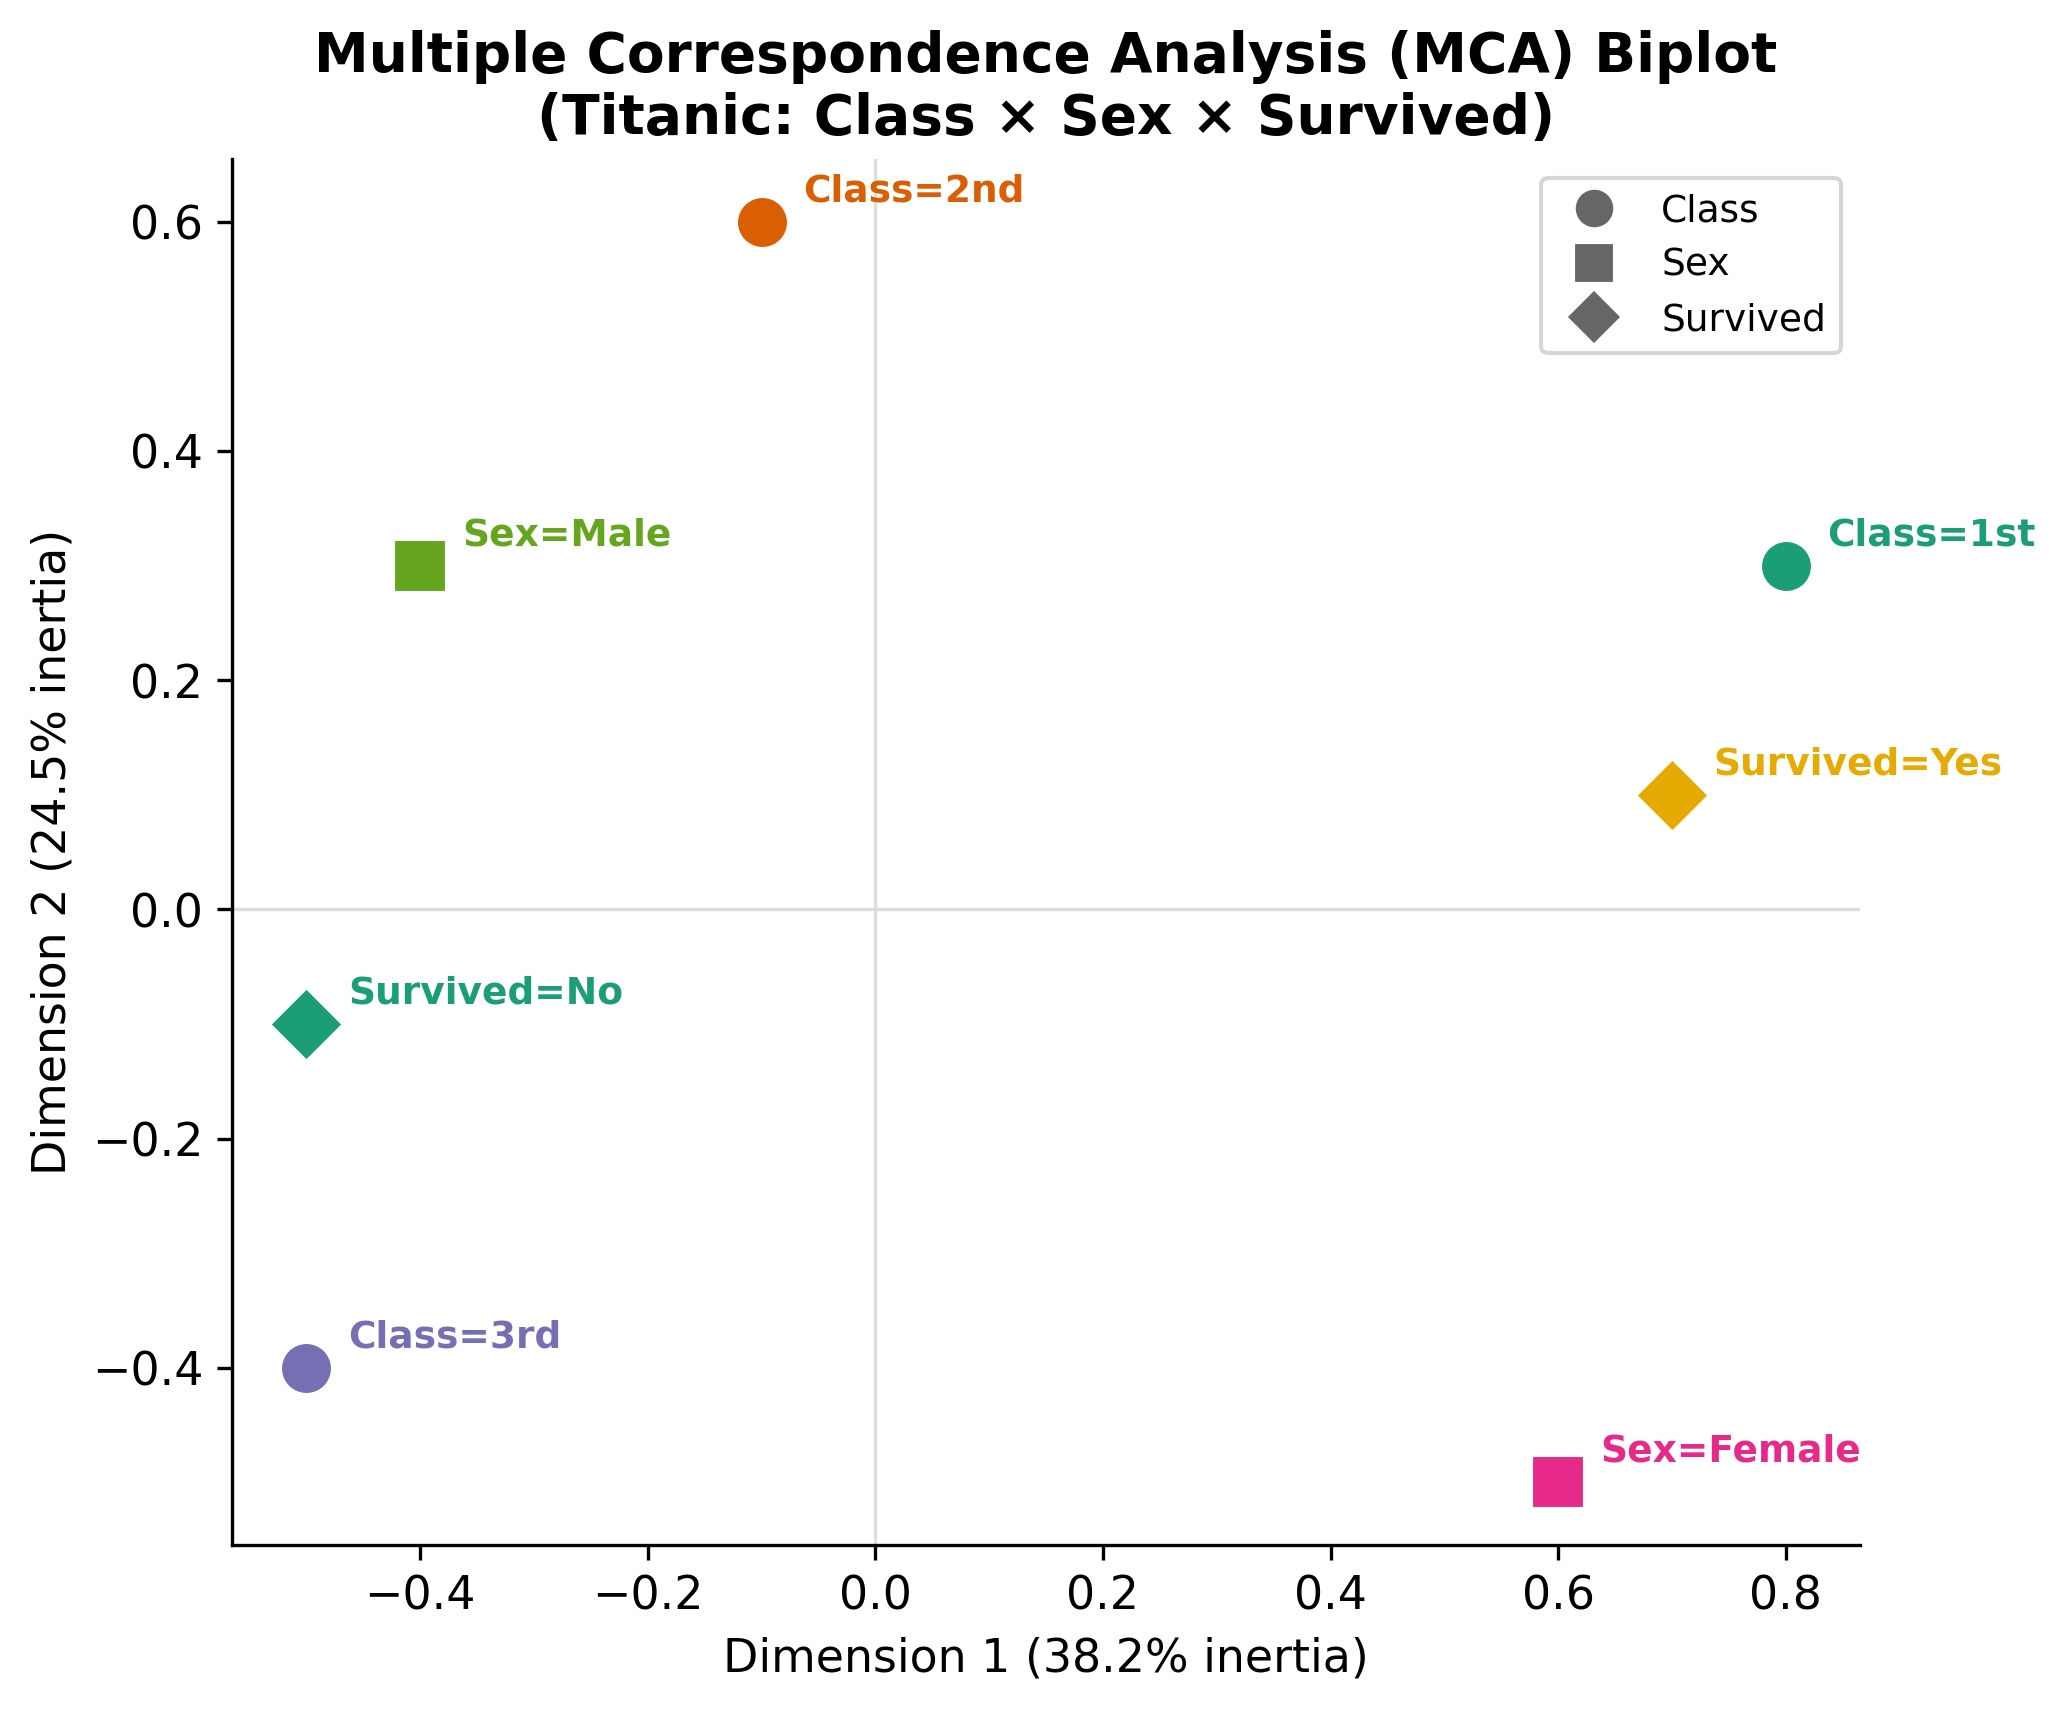
\includegraphics[width=\textwidth]{m3_5_mca_biplot.png}
\begin{exampleblock}{Data Insight}
    \scriptsize \texttt{prince.MCA()} follows the scikit-learn API: \texttt{fit()}, \texttt{transform()}, \texttt{row\_coordinates()}, \texttt{column\_coordinates()}. Use different markers per original variable for clarity.
\end{exampleblock}
\end{column}
\end{columns}
\end{frame}

% ── 139 ──
\begin{frame}{Supplementary Points}
\smark{139/300}
\begin{columns}[T]
\begin{column}{0.50\textwidth}
\begin{itemize}
    \item \textbf{Active points}: used in computing the CA/MCA dimensions
    \item \textbf{Supplementary points}: projected into the space \emph{after} the dimensions are computed
    \item Supplementary rows or columns do not influence the axes
    \item Use for: rare categories, new groups, continuous variables (as supplementary quantitative)
\end{itemize}
\end{column}
\begin{column}{0.47\textwidth}
\begin{alertblock}{Pro-Tip}
    \scriptsize R: \texttt{CA(ct, row.sup=5)} makes the 5th row supplementary. \texttt{MCA(df, quali.sup=4)} makes the 4th variable supplementary. Supplementary points are typically plotted in a different color/shape (e.g., dashed outline).
\end{alertblock}
\vspace{0.1cm}
\begin{exampleblock}{Data Insight}
    \scriptsize Supplementary variables act as ``labels'' on the map: they show where new or external categories would fall without distorting the existing structure. Essential for holdout validation of the CA solution.
\end{exampleblock}
\end{column}
\end{columns}
\end{frame}

% ── 140 ──
\begin{frame}[fragile]{Supplementary Points --- Code}\smark{140/300}
\begin{columns}[T]
\begin{column}{0.48\textwidth}
\begin{lstlisting}[style=Rstyle]
# CA with supplementary row
ca_sup <- CA(ct,
  row.sup = 4,  # 4th row = supp
  col.sup = NULL)

# MCA with supplementary variable
mca_sup <- MCA(titanic_cat,
  quali.sup = 3)  # 3rd var = supp

# Plot: supplementary in italic
fviz_ca_biplot(ca_sup,
  repel = TRUE)
# Supplementary points auto-styled

# Access coordinates
ca_sup$row.sup$coord
\end{lstlisting}
\end{column}
\begin{column}{0.48\textwidth}
\begin{lstlisting}[style=Pystyle]
# prince: fit on active, then
# transform supplementary
mca = prince.MCA(n_components=2)
mca = mca.fit(active_vars)

# Project supplementary
sup_coords = mca.transform(
    sup_data)

# Plot active + supplementary
ax.scatter(active_x, active_y,
    color="#2166AC", label="Active")
ax.scatter(sup_coords[0],
    sup_coords[1],
    color="#999", marker="x",
    s=80, label="Supplementary")
ax.legend()
\end{lstlisting}
\end{column}
\end{columns}
\end{frame}

% ── 141 ──
\begin{frame}{Biplot Normalization: Symmetric vs.\ Asymmetric}
\smark{141/300}
\centering\small
\begin{tabular}{@{}llll@{}}
    \toprule
    \textbf{Normalization} & \textbf{Row coords} & \textbf{Col coords} & \textbf{Interpretation} \\
    \midrule
    Symmetric (default)     & Principal $\times \sqrt{\lambda}$ & Principal $\times \sqrt{\lambda}$ & Row-col proximity = approx.\ assoc. \\
    Row principal           & Principal                 & Standard               & Row distances are exact $\chi^2$ \\
    Column principal        & Standard                  & Principal               & Column distances are exact $\chi^2$ \\
    Standard                & Standard                  & Standard               & Inner product = exact $\chi^2$ \\
    \bottomrule
\end{tabular}

\vspace{0.3cm}
\begin{alertblock}{Pro-Tip}
    \scriptsize \textbf{Symmetric} (default in most packages) is best for general exploration. Use \textbf{row principal} when the research question is about row categories, and vice versa. Always state which normalization was used in the figure caption.
\end{alertblock}
\end{frame}

% ── 142 ──
\begin{frame}{CA for Large Tables}
\smark{142/300}
\begin{columns}[T]
\begin{column}{0.50\textwidth}
\begin{itemize}
    \item Tables with 20+ rows or columns produce cluttered biplots
    \item Strategies: show only top-$k$ contributors; grey out low-$\cos^2$ points; label only outliers
    \item For very large tables (e.g., text analysis: documents $\times$ words), CA becomes a core exploratory tool
    \item Cluster the biplot coordinates with $k$-means for grouping
\end{itemize}
\end{column}
\begin{column}{0.47\textwidth}
\begin{alertblock}{Pro-Tip}
    \scriptsize R: \texttt{fviz\_ca\_biplot(ca\_result, select.row=list(contrib=10))} shows only the top 10 contributing row points. Python: filter coordinates by contribution threshold before plotting.
\end{alertblock}
\vspace{0.1cm}
\begin{exampleblock}{Data Insight}
    \scriptsize CA on a document-term matrix is sometimes called ``Latent Semantic Analysis'' (LSA). The biplot shows which documents cluster near which terms --- a visual topic model.
\end{exampleblock}
\end{column}
\end{columns}
\end{frame}

% ── 143 ──
\begin{frame}{CA vs.\ Other Categorical Visualizations}
\smark{143/300}
\centering\small
\begin{tabular}{@{}llll@{}}
    \toprule
    \textbf{Display} & \textbf{Variables} & \textbf{Shows} & \textbf{Best For} \\
    \midrule
    Mosaic              & 2 (--3)   & Marginals + conditionals    & Joint distribution \\
    Association plot    & 2         & Residuals from independence  & Specific deviations \\
    Heatmap             & 2         & Cell values                  & Exact numbers \\
    Alluvial            & 2--4      & Flow between categories      & Partitioning \\
    CA biplot           & 2 (via table)& Latent structure           & Row-column association \\
    MCA biplot          & 3+        & Multi-variable co-occurrence & Pattern discovery \\
    \bottomrule
\end{tabular}

\vspace{0.3cm}
\begin{exampleblock}{Data Insight}
    \scriptsize CA adds value when the table is large ($> 5 \times 5$) or when the goal is \emph{pattern discovery} rather than \emph{hypothesis testing}. For $2 \times 2$ or $2 \times 3$ tables, the mosaic + residual shading is sufficient.
\end{exampleblock}
\end{frame}

% ── 144 ──
\begin{frame}{Enhancing the Biplot}
\smark{144/300}
\begin{columns}[T]
\begin{column}{0.50\textwidth}
    \textbf{Visual enhancements:}
    \begin{itemize}
        \item Color by $\cos^2$ (quality)
        \item Size by contribution
        \item Ellipses around groups (confidence or convex hull)
        \item Arrows from origin for column points
        \item Supplementary variables as labels only
    \end{itemize}
\end{column}
\begin{column}{0.47\textwidth}
    \textbf{Annotation:}
    \begin{itemize}
        \item Axis labels: ``Dim 1 (89.4\% inertia)''
        \item Caption: $\chi^2$ test result + total inertia
        \item Legend distinguishing rows vs.\ columns
        \item Note which normalization was used
    \end{itemize}
    \vspace{0.1cm}
    \begin{alertblock}{Pro-Tip}
        \scriptsize R: \texttt{fviz\_ca\_biplot(ca\_result, col.row="cos2", repel=TRUE, addEllipses=TRUE)} adds confidence ellipses. Python: use \texttt{matplotlib.patches.Ellipse} manually.
    \end{alertblock}
\end{column}
\end{columns}
\end{frame}

% ── 145 ──
\begin{frame}[fragile]{Enhanced Biplot --- Code}\smark{145/300}
\begin{columns}[T]
\begin{column}{0.48\textwidth}
\begin{lstlisting}[style=Rstyle]
# Color by quality (cos2)
fviz_ca_biplot(ca_result,
  col.row = "cos2",
  col.col = "cos2",
  gradient.cols = c("#EEEEEE",
    "#2166AC", "#B2182B"),
  repel = TRUE,
  shape.row = 16,
  shape.col = 17,
  pointsize = "contrib") +
  labs(title="CA: Hair x Eye",
    caption=paste0(
      "Total inertia = ",
      round(sum(ca_result$eig[,1]),3),
      ", chi2 p < 0.001")) +
  theme_minimal()
\end{lstlisting}
\end{column}
\begin{column}{0.48\textwidth}
\begin{lstlisting}[style=Pystyle]
fig, ax = plt.subplots(figsize=(7,6))

# Rows: color by cos2, size by contrib
cos2_r = row_cos2.sum(axis=1)
contrib_r = row_contrib.iloc[:,0]*500

sc = ax.scatter(F[:,0], F[:,1],
    c=cos2_r, s=contrib_r,
    cmap="RdYlBu_r", vmin=0, vmax=1,
    marker="o", edgecolors="white")

# Columns: triangles
ax.scatter(G[:,0], G[:,1],
    marker="^", s=100, color="#B2182B")

plt.colorbar(sc, label="cos²")
ax.set_xlabel(f"Dim 1 ({pct1:.1f}%)")
ax.set_ylabel(f"Dim 2 ({pct2:.1f}%)")
\end{lstlisting}
\end{column}
\end{columns}
\end{frame}

% ── 146 ──
\begin{frame}{CA Assumptions and Caveats}
\smark{146/300}
\begin{columns}[T]
\begin{column}{0.50\textwidth}
\begin{itemize}
    \item CA assumes the $\chi^2$ model is meaningful (expected counts $\geq 5$)
    \item Outlier categories (very rare) can dominate the first dimension
    \item CA is exploratory, not confirmatory --- no $p$-values on the biplot
    \item The total inertia = $\chi^2 / N$: if $\chi^2$ is not significant, the CA map is noise
\end{itemize}
\end{column}
\begin{column}{0.47\textwidth}
\begin{alertblock}{Pro-Tip}
    \scriptsize Always run the $\chi^2$ test \textbf{first}. If $p > 0.05$, the CA biplot is not interpretable --- there is no association to decompose. Report $\chi^2(df) = X$, $p < \alpha$ alongside the biplot.
\end{alertblock}
\vspace{0.1cm}
\begin{exampleblock}{Data Insight}
    \scriptsize Rare categories with $< 5\%$ of the total can be merged into ``Other'' or treated as supplementary. Otherwise, their extreme profiles dominate the map and mask the main structure.
\end{exampleblock}
\end{column}
\end{columns}
\end{frame}

% ── 147 ──
\begin{frame}{MCA Extensions and Variants}
\smark{147/300}
\centering\small
\begin{tabular}{@{}lll@{}}
    \toprule
    \textbf{Method} & \textbf{Use Case} & \textbf{R / Python} \\
    \midrule
    CA (simple)   & 2 categorical variables        & \texttt{FactoMineR::CA} / \texttt{prince.CA} \\
    MCA           & 3+ categorical variables       & \texttt{FactoMineR::MCA} / \texttt{prince.MCA} \\
    FAMD          & Mixed (categorical + continuous)& \texttt{FactoMineR::FAMD} / \texttt{prince.FAMD} \\
    Specific MCA  & MCA adjusted for dimensionality& \texttt{FactoMineR::MCA} (adj.\ inertia) \\
    Joint CA      & Multiple tables                & \texttt{FactoMineR::MFA} \\
    \bottomrule
\end{tabular}

\vspace{0.3cm}
\begin{exampleblock}{Data Insight}
    \scriptsize FAMD (Factor Analysis of Mixed Data) handles both numeric and categorical variables in a single analysis. It is the ``universal'' dimension reduction for mixed survey data. Module 5.4 covers PCA; FAMD bridges PCA and MCA.
\end{exampleblock}
\end{frame}

% ── 148 ──
\begin{frame}{CA Package Ecosystem}
\smark{148/300}
\centering\small
\begin{tabular}{@{}lll@{}}
    \toprule
    \textbf{Task} & \textbf{R} & \textbf{Python} \\
    \midrule
    Simple CA          & \texttt{FactoMineR::CA()}        & \texttt{prince.CA()} \\
    MCA                & \texttt{FactoMineR::MCA()}       & \texttt{prince.MCA()} \\
    FAMD               & \texttt{FactoMineR::FAMD()}      & \texttt{prince.FAMD()} \\
    Visualization      & \texttt{factoextra::fviz\_*()}   & Manual matplotlib / plotly \\
    Scree plot         & \texttt{fviz\_screeplot()}       & Manual bar chart \\
    Contributions      & \texttt{fviz\_contrib()}         & Manual from \texttt{.contributions\_} \\
    cos$^2$            & \texttt{fviz\_cos2()}            & Manual from \texttt{.cosine\_similarities()} \\
    Base R CA          & \texttt{ca::ca()}                & --- \\
    3D biplot          & \texttt{scatterplot3d} + CA      & \texttt{plotly} 3D scatter \\
    \bottomrule
\end{tabular}
\end{frame}

% ── 149 ──
\begin{frame}{CA Decision Guide}
\smark{149/300}
\centering\small
\begin{tabular}{@{}lll@{}}
    \toprule
    \textbf{Data} & \textbf{Method} & \textbf{When} \\
    \midrule
    $r \times c$ table ($< 5 \times 5$)    & Mosaic + residuals   & Direct interpretation \\
    $r \times c$ table ($\geq 5 \times 5$) & CA biplot            & Pattern discovery \\
    3+ categorical variables                & MCA                  & Multi-variable structure \\
    Mixed (cat + numeric)                   & FAMD                 & Survey analysis \\
    Multiple tables                         & MFA                  & Multi-group comparison \\
    Text (documents $\times$ words)         & CA / LSA             & Topic exploration \\
    \bottomrule
\end{tabular}

\vspace{0.3cm}
\begin{alertblock}{Pro-Tip}
    \scriptsize CA is underused in practice. For any $\chi^2$-significant table larger than $3 \times 3$, the CA biplot reveals structure that the mosaic plot cannot --- especially clusters of co-associated categories.
\end{alertblock}
\end{frame}

% ── 150 ──
\begin{frame}{Module 3.5 --- Key Takeaways}\smark{150/300}
\begin{enumerate}
    \item \textbf{CA} projects rows and columns of a contingency table into a shared low-dimensional space.
    \item \textbf{Proximity on the biplot $\approx$ association} in the table.
    \item \textbf{Inertia} decomposes the total $\chi^2$; scree plot selects dimensions.
    \item \textbf{Contributions} identify which categories define each dimension.
    \item \textbf{cos$^2$} flags poorly represented points --- grey them out.
    \item \textbf{MCA} extends CA to 3+ categorical variables; \textbf{FAMD} handles mixed data.
\end{enumerate}
\end{frame}

% ── 151 ──
\begin{frame}{}\smark{151/300}
\centering\vspace{1.5cm}
{\Large\textbf{Module 3.5 Complete}}\\[0.5cm]
You can now perform and visualize Correspondence Analysis and MCA --- with biplots, scree plots, contribution charts, and cos$^2$ quality checks --- turning contingency tables into maps of categorical association.\\[0.5cm]
\textbf{Next:} Module 3.6 --- Ordinal Data, Cumulative Plots, and Rating Distributions.
\end{frame}

% ═══════════════════════════════════════════════════════
%  MODULE 3.6 — Ordinal Data, Cumulative Plots, and Rating Distributions
% ═══════════════════════════════════════════════════════
\section{Module 3.6 --- Ordinal Data and Cumulative Plots}

% ── 152 ──
\begin{frame}{Module 3.6 --- Roadmap}\smark{152/300}
\begin{enumerate}
    \item Ordinal vs.\ nominal: what the order buys you
    \item Cumulative distribution plots for ordinal data
    \item Diverging stacked bars for rating comparison
    \item Median + IQR for ordinal summaries
    \item Ridgelines for ordinal distributions
    \item Proportional dot matrices (icon arrays)
    \item Cumulative odds and the proportional odds model
    \item Heat strips for multi-item ordinal profiles
\end{enumerate}
\end{frame}

% ── 153 ──
\begin{frame}{Ordinal vs.\ Nominal: What the Order Buys You}
\smark{153/300}
\begin{columns}[T]
\begin{column}{0.50\textwidth}
\begin{itemize}
    \item \textbf{Nominal}: categories have no intrinsic order. Sort by value.
    \item \textbf{Ordinal}: categories have a natural sequence. \textbf{Preserve it.}
    \item Ordinal order enables: cumulative distributions, medians, rank tests, proportional odds models
    \item Violating order (sorting ``Good'' before ``Fair'') destroys the data's structure
\end{itemize}
\end{column}
\begin{column}{0.47\textwidth}
\begin{alertblock}{Pro-Tip}
    \scriptsize In R: \texttt{factor(x, levels=c("VP","P","F","G","E"), ordered=TRUE)}. In Python: \texttt{pd.Categorical(x, categories=[...], ordered=True)}. The \texttt{ordered=TRUE} flag tells downstream functions to respect the sequence.
\end{alertblock}
\vspace{0.1cm}
\begin{exampleblock}{Data Insight}
    \scriptsize Many datasets encode ordinal variables as integers (1--5). This is convenient for computing means but obscures the categorical nature. Always label the levels on visualizations.
\end{exampleblock}
\end{column}
\end{columns}
\end{frame}

% ── 154 ──
\begin{frame}{Cumulative Distribution Plot}
\smark{154/300}
\centering
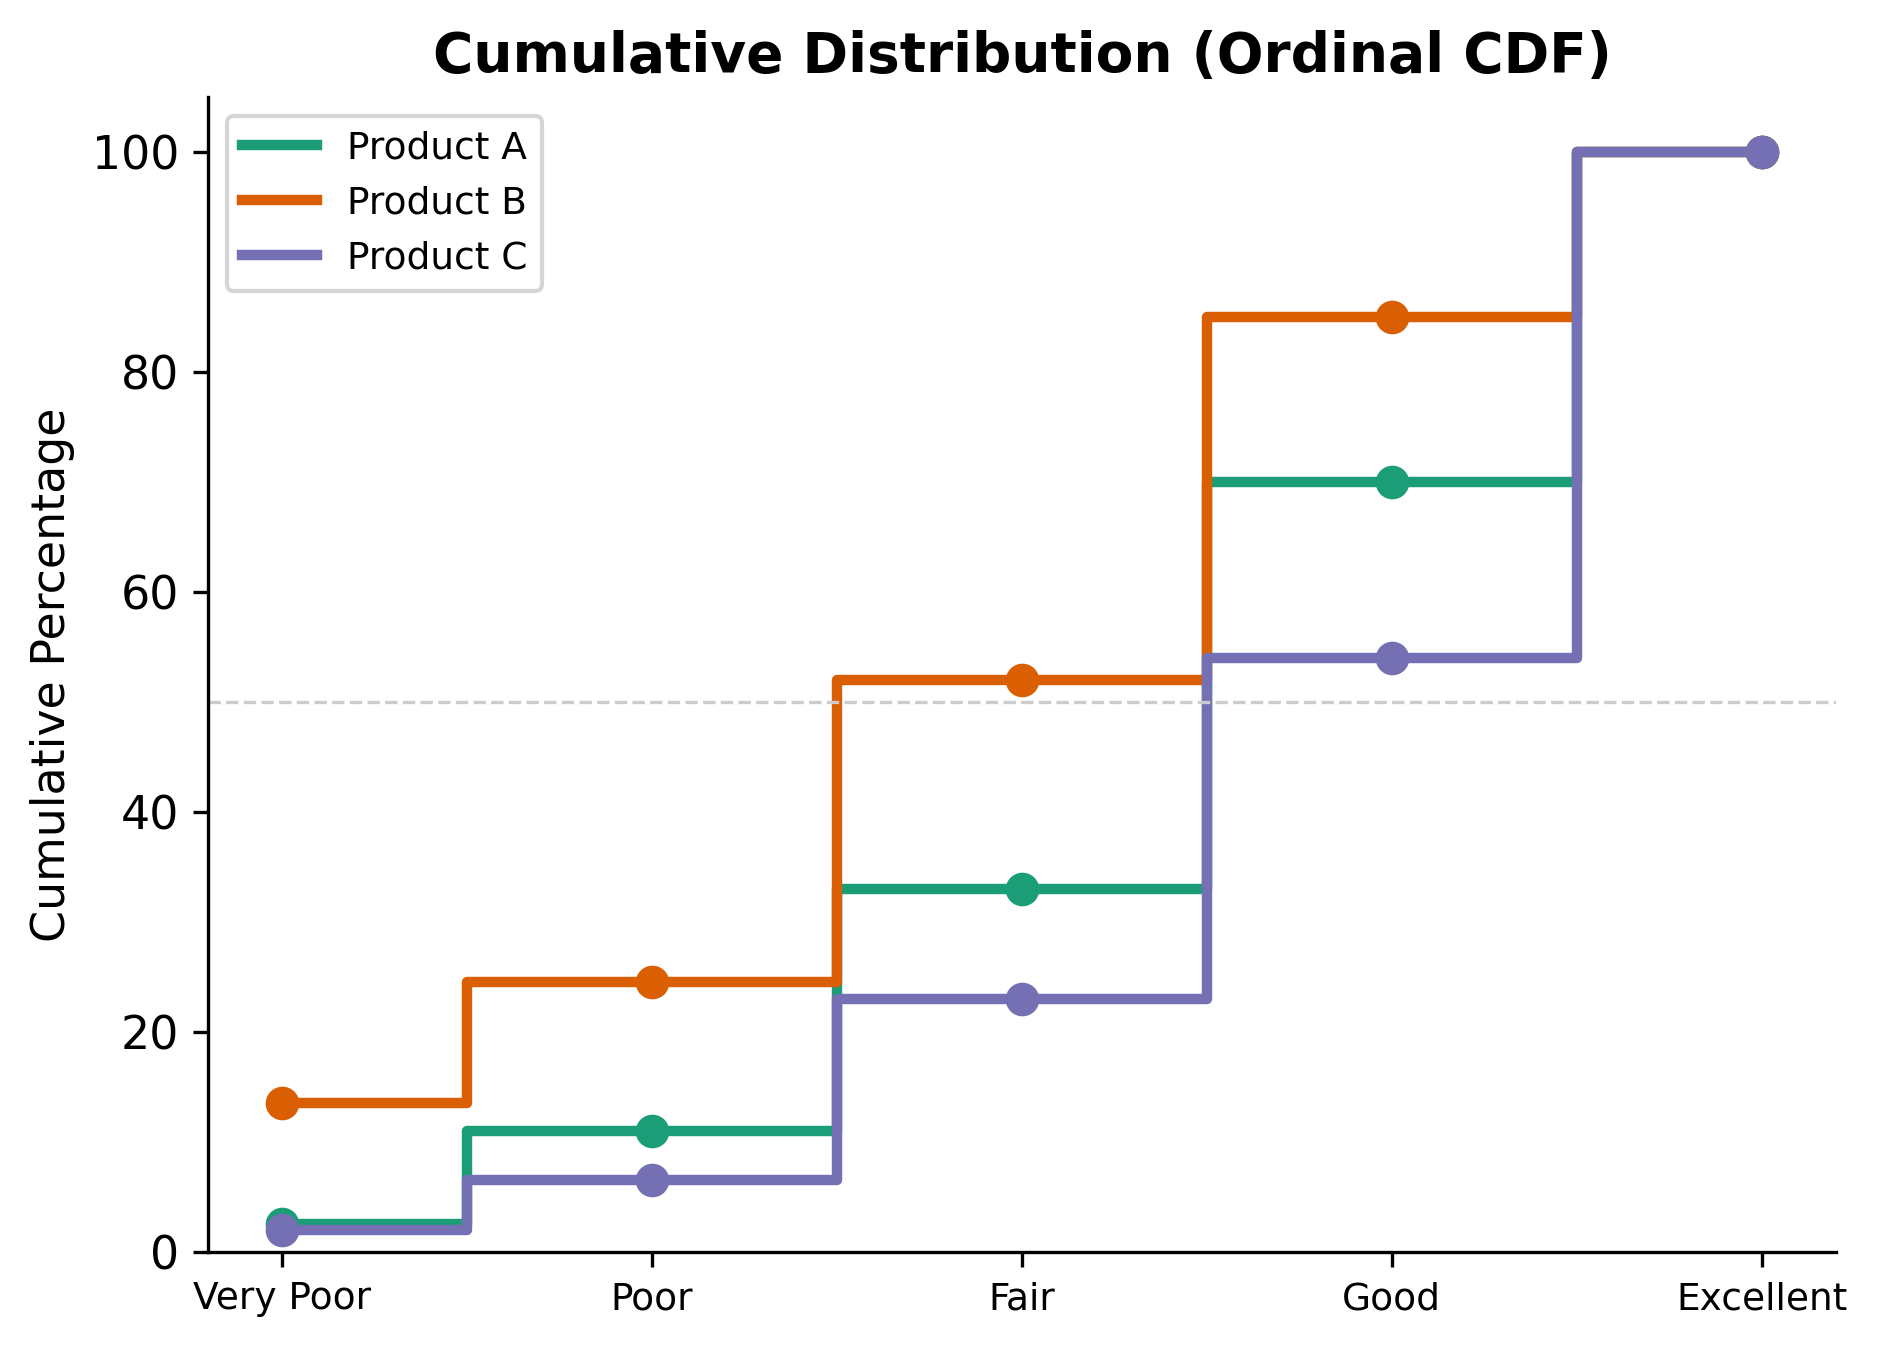
\includegraphics[width=0.72\textwidth]{m3_6_cumulative.png}

\vspace{0.2cm}
\begin{columns}[T]
\begin{column}{0.48\textwidth}
\begin{itemize}
    \item $y$-axis: $P(Y \leq j)$ for each ordinal level $j$
    \item Step function: rises at each category
    \item Reaches 100\% at the highest level
    \item \textbf{Stochastic dominance}: a curve that is everywhere \textbf{lower} represents a better distribution
    \item The 50\% line locates the median
\end{itemize}
\end{column}
\begin{column}{0.48\textwidth}
\begin{exampleblock}{Data Insight}
    \scriptsize Product C (purple) is everywhere below A and B --- it stochastically dominates. At ``Fair,'' only 23\% of C responses are $\leq$Fair vs.\ 52\% of B. The cumulative plot reveals this dominance relationship directly.
\end{exampleblock}
\end{column}
\end{columns}
\end{frame}

% ── 155 ──
\begin{frame}[fragile]{Cumulative Distribution --- \Rlang}\smark{155/300}
\begin{columns}[T]
\begin{column}{0.55\textwidth}
\begin{lstlisting}[style=Rstyle]
# Compute cumulative proportions
cum_df <- df |>
  group_by(product, rating) |>
  summarise(n = n()) |>
  mutate(pct = n / sum(n),
         cum_pct = cumsum(pct))

ggplot(cum_df,
  aes(rating, cum_pct,
      color = product,
      group = product)) +
  geom_step(linewidth = 1.5) +
  geom_point(size = 3) +
  geom_hline(yintercept = 0.5,
    linetype = "dashed",
    color = "#CCC") +
  scale_y_continuous(
    labels = scales::percent) +
  theme_minimal()
\end{lstlisting}
\end{column}
\begin{column}{0.42\textwidth}
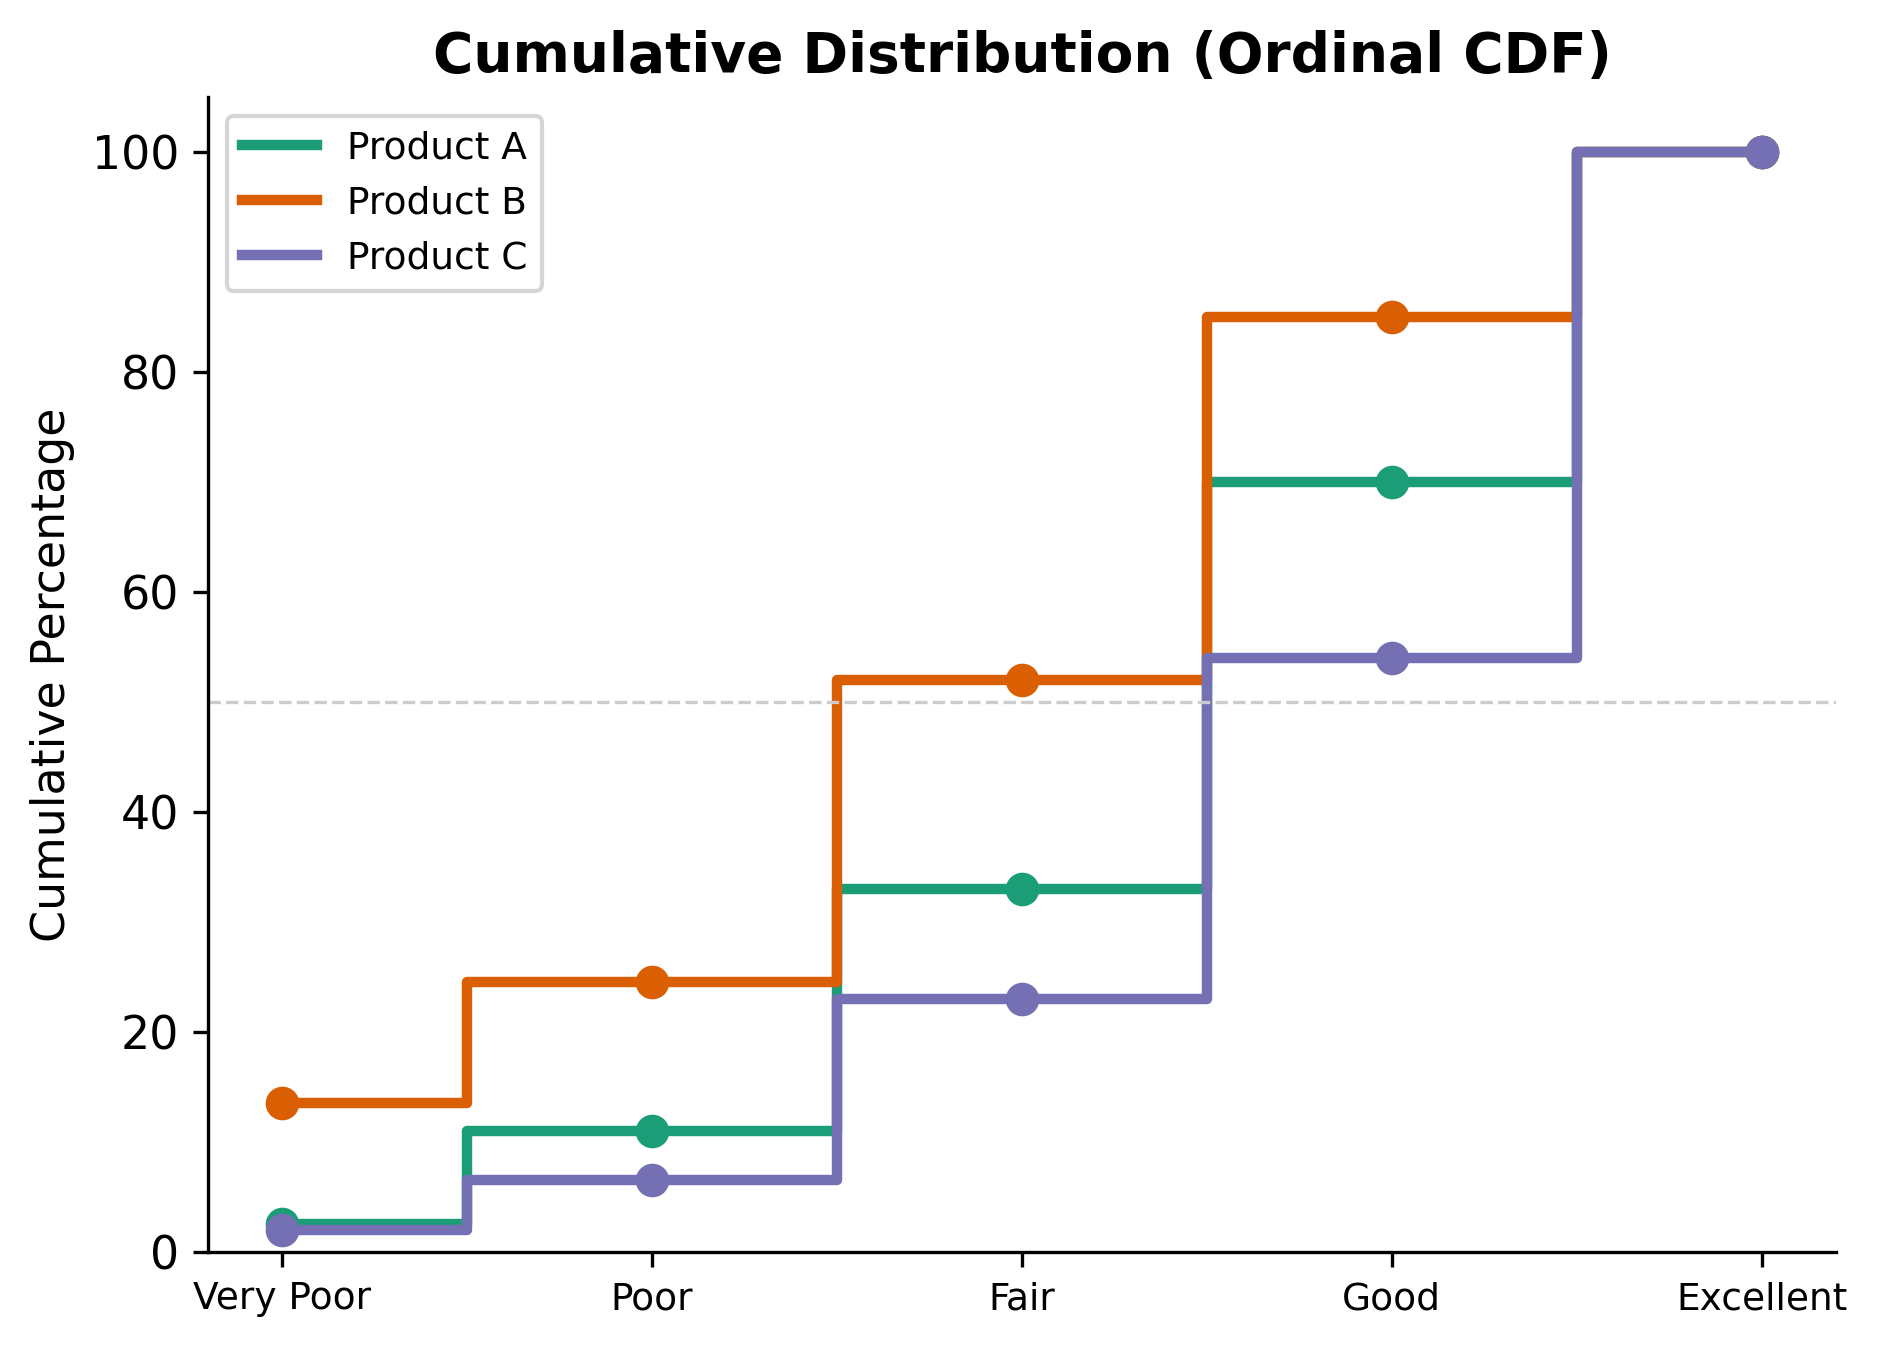
\includegraphics[width=\textwidth]{m3_6_cumulative.png}
\begin{alertblock}{Pro-Tip}
    \scriptsize \texttt{geom\_step()} is the correct geom for ordinal CDFs --- it shows discrete jumps at each level. \texttt{geom\_line()} implies continuous interpolation between levels, which is misleading for ordinal data.
\end{alertblock}
\end{column}
\end{columns}
\end{frame}

% ── 156 ──
\begin{frame}[fragile]{Cumulative Distribution --- \Python}\smark{156/300}
\begin{columns}[T]
\begin{column}{0.55\textwidth}
\begin{lstlisting}[style=Pystyle]
# Manual step plot
for prod, c in zip(products, colors):
    sub = df[df["product"]==prod]
    counts = sub["rating"]\
        .value_counts().sort_index()
    cum_pct = counts.cumsum() / \
        counts.sum() * 100
    ax.step(range(len(levels)),
        cum_pct.values,
        where="mid", color=c,
        linewidth=2.5, label=prod)
    ax.scatter(range(len(levels)),
        cum_pct.values,
        color=c, s=50, zorder=5)

ax.set_xticks(range(5))
ax.set_xticklabels(levels)
ax.axhline(50, linestyle="--",
    color="#CCC")
ax.legend()
\end{lstlisting}
\end{column}
\begin{column}{0.42\textwidth}
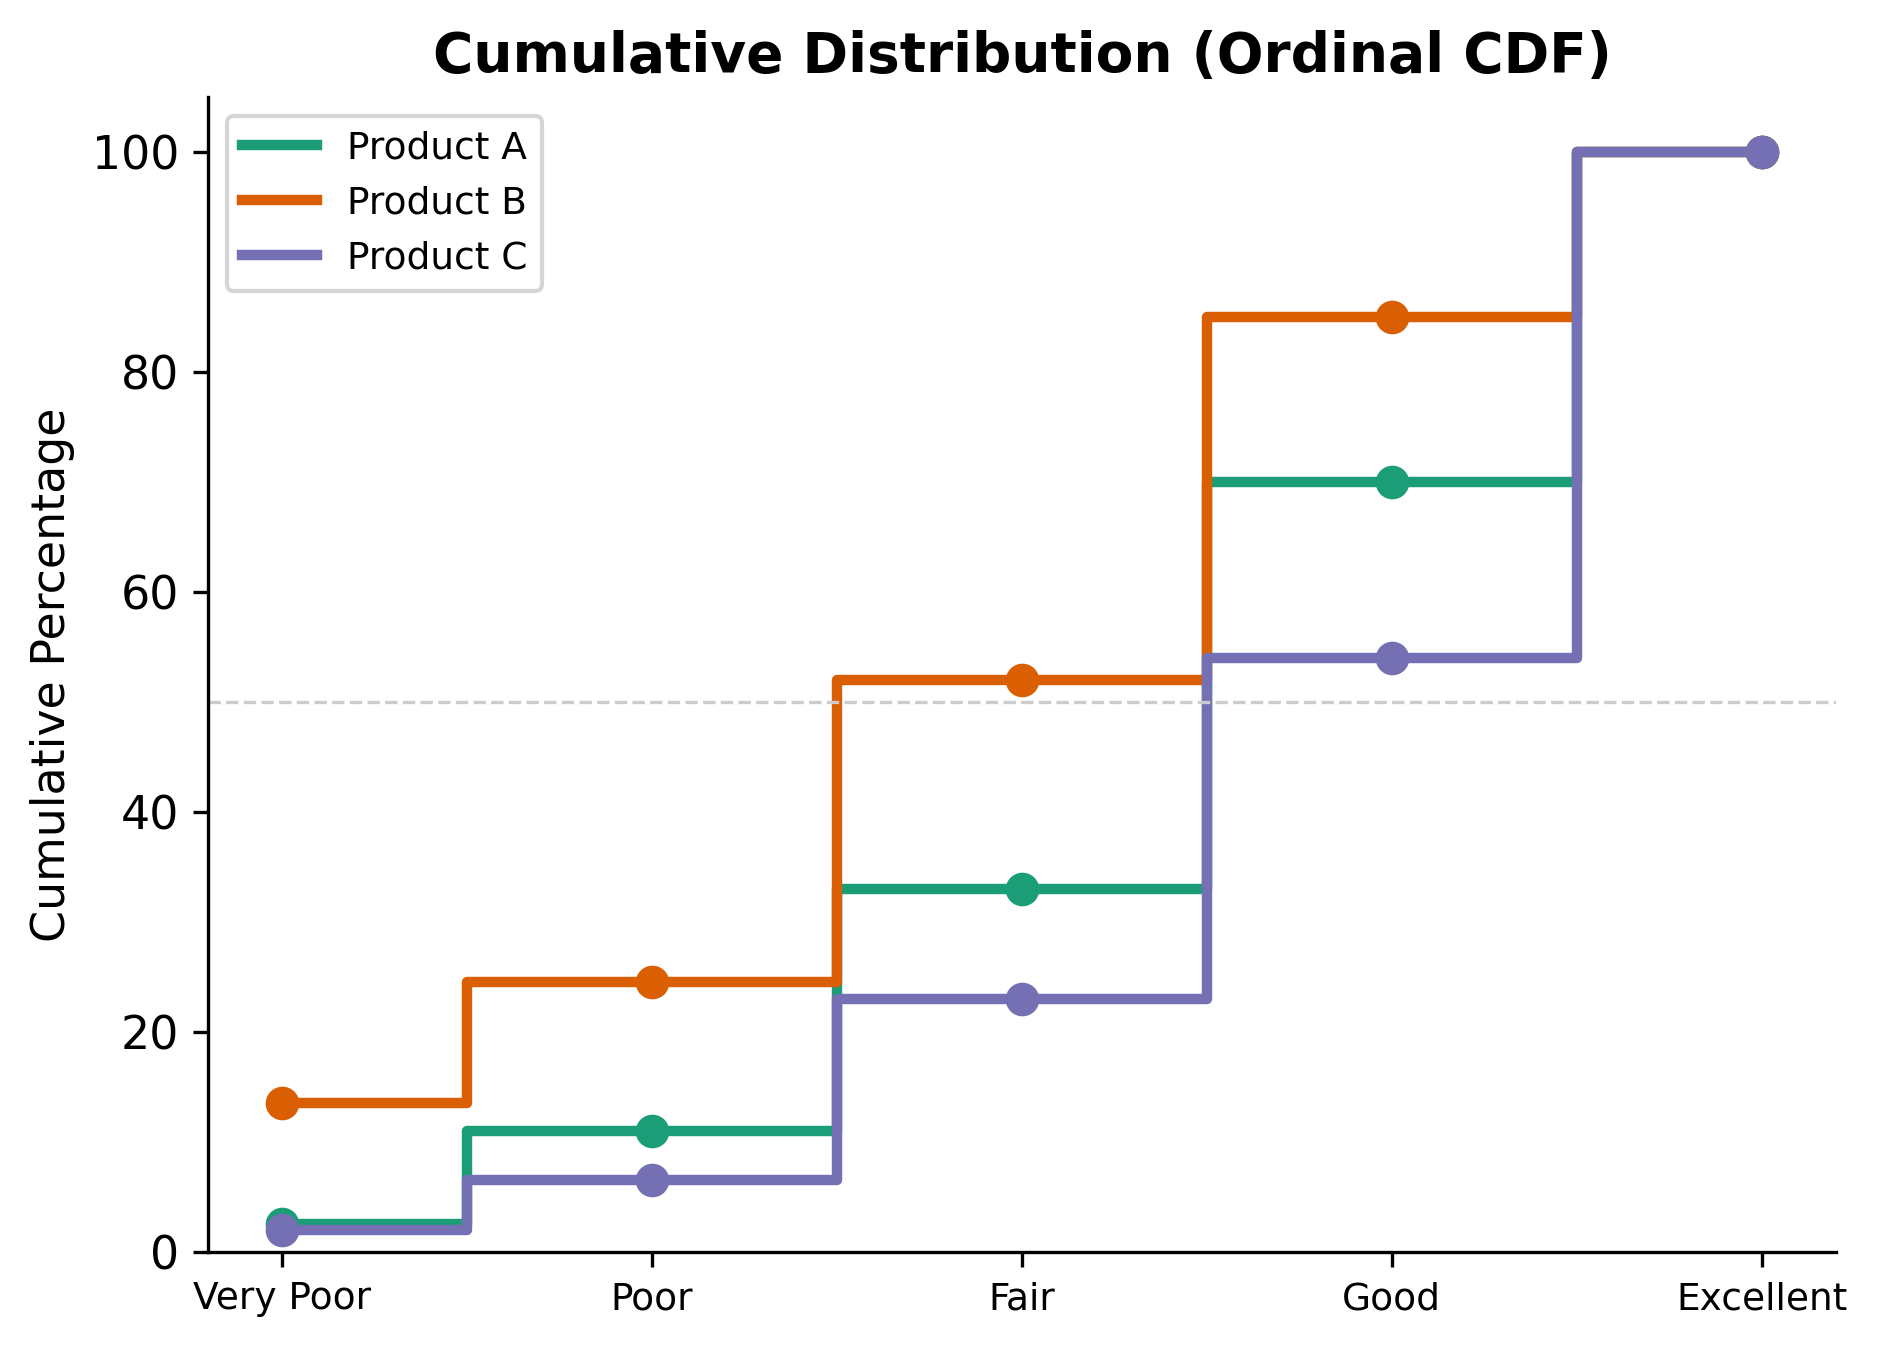
\includegraphics[width=\textwidth]{m3_6_cumulative.png}
\begin{exampleblock}{Data Insight}
    \scriptsize In Python, use \texttt{ax.step(where="mid")} for the step CDF. \texttt{np.cumsum(counts) / total} computes the empirical CDF. Overlay multiple products for direct comparison.
\end{exampleblock}
\end{column}
\end{columns}
\end{frame}

% ── 157 ──
\begin{frame}{Stochastic Dominance: Visual Ranking}
\smark{157/300}
\begin{columns}[T]
\begin{column}{0.50\textwidth}
\begin{itemize}
    \item Product A \textbf{first-order stochastically dominates} B if $F_A(j) \leq F_B(j)$ for all $j$
    \item Visually: A's cumulative curve is everywhere \textbf{below} B's
    \item If curves cross: no dominance --- the comparison depends on which levels you weight
    \item The Kolmogorov--Smirnov test formalizes this: max $|F_A - F_B|$
\end{itemize}
\end{column}
\begin{column}{0.47\textwidth}
\begin{exampleblock}{Data Insight}
    \scriptsize Stochastic dominance is a \textbf{stronger} claim than ``higher mean.'' If A dominates B, then any monotone transformation of the scale preserves A's superiority. The mean comparison requires interval-level assumptions; dominance does not.
\end{exampleblock}
\vspace{0.1cm}
\begin{alertblock}{Pro-Tip}
    \scriptsize R: \texttt{ks.test(data\_A, data\_B)} for the KS test. Python: \texttt{scipy.stats.ks\_2samp()}. The $p$-value tests whether the CDFs differ significantly.
\end{alertblock}
\end{column}
\end{columns}
\end{frame}

% ── 158 ──
\begin{frame}{Diverging Stacked Bars for Rating Comparison}
\smark{158/300}
\centering
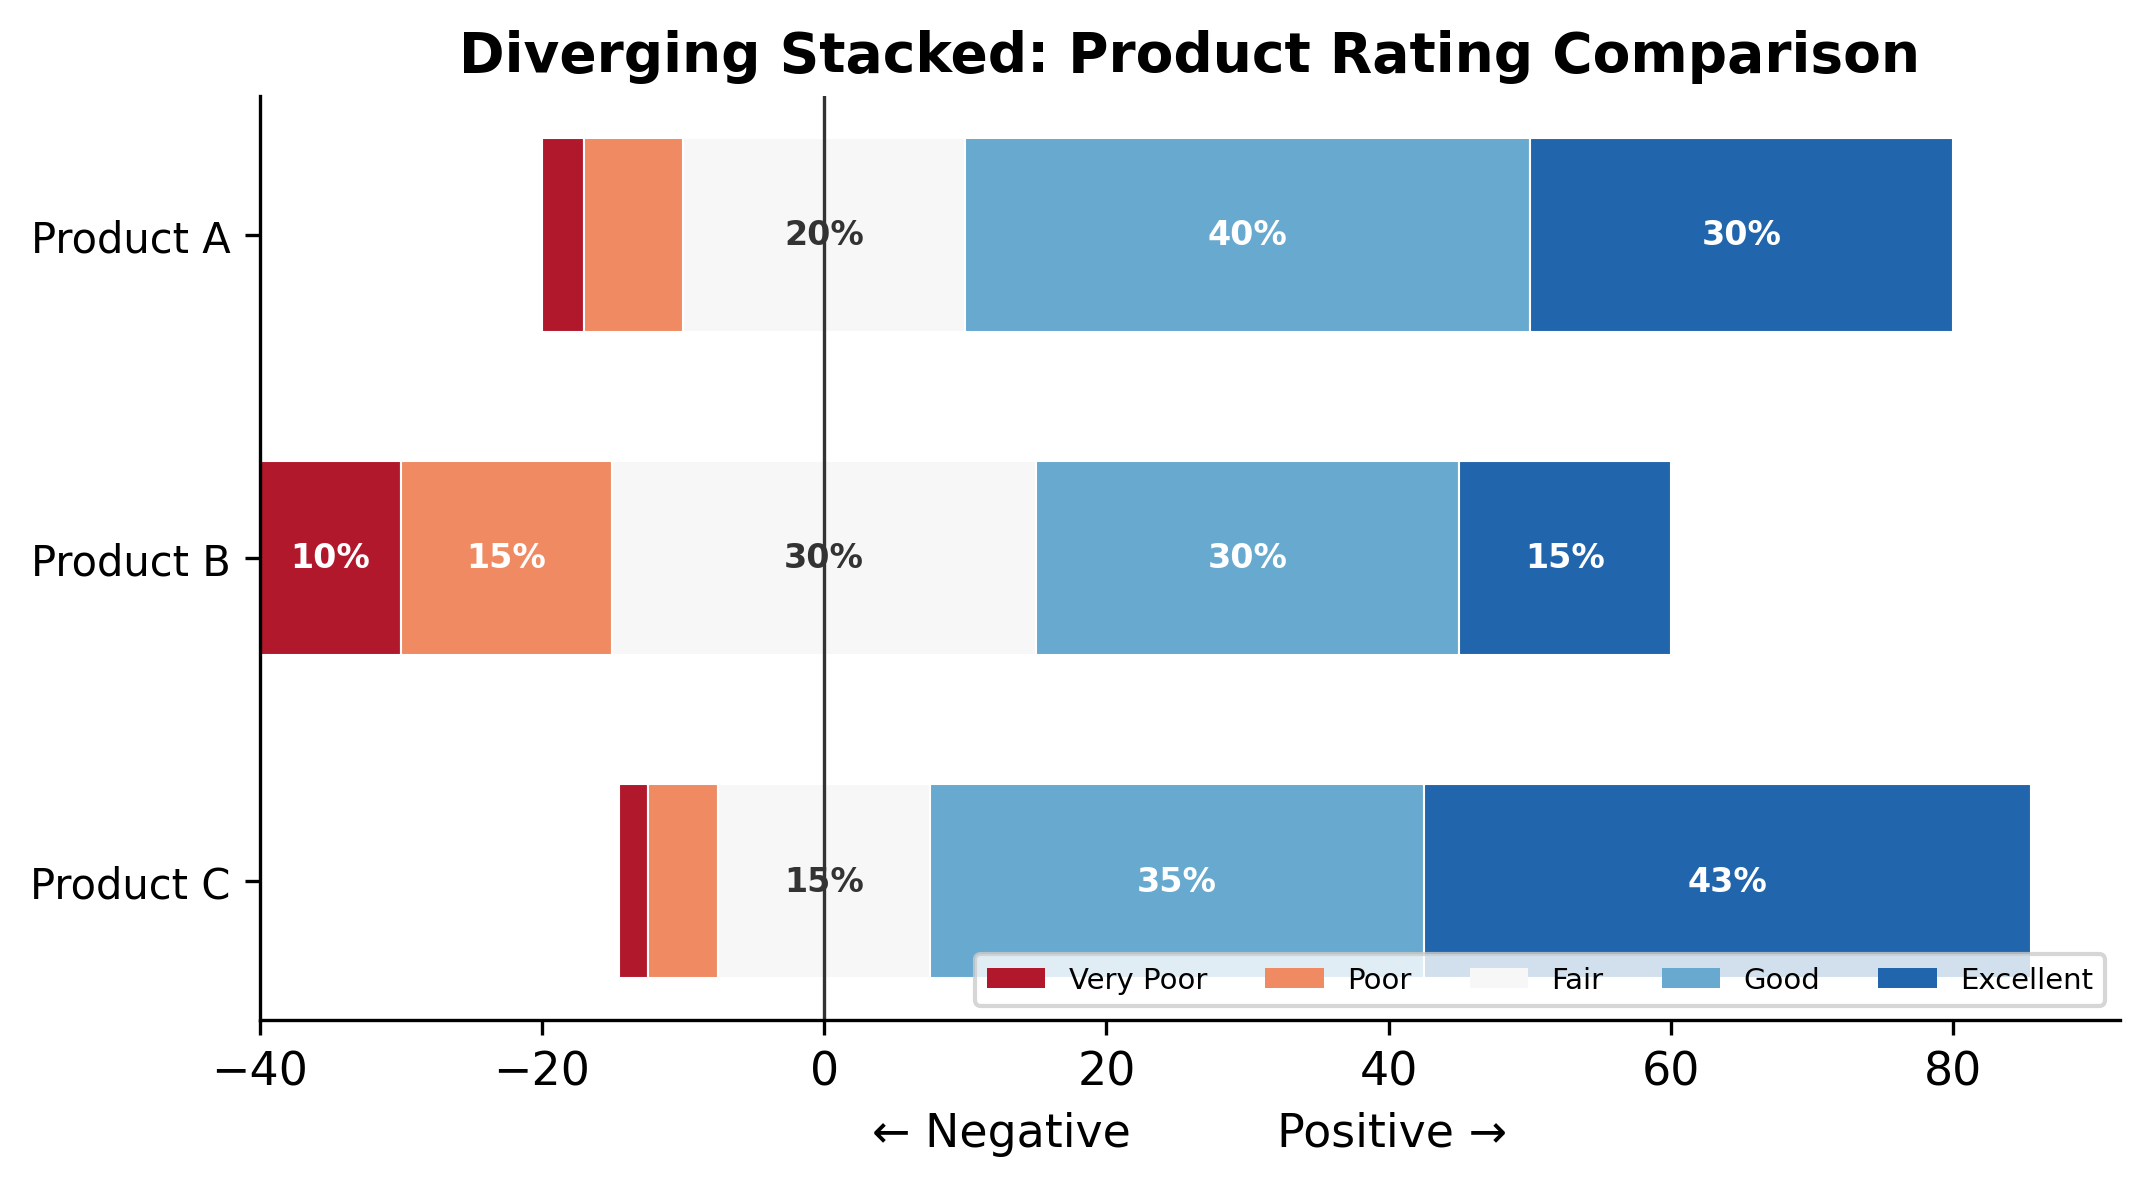
\includegraphics[width=0.78\textwidth]{m3_6_product_compare.png}

\vspace{0.2cm}
\begin{exampleblock}{Data Insight}
    \scriptsize Product C extends furthest right (most Excellent). Product B is the most left-shifted (most negative). The diverging format shows both the direction and magnitude of rating differences in a compact display --- ideal for comparing 3--10 items on the same ordinal scale.
\end{exampleblock}
\end{frame}

% ── 159 ──
\begin{frame}[fragile]{Rating Comparison --- Code}\smark{159/300}
\begin{columns}[T]
\begin{column}{0.48\textwidth}
\begin{lstlisting}[style=Rstyle]
# Same as Module 3.4 diverging bar
# but with products as rows
library(likert)
lik <- likert(items_df)
plot(lik, centered=TRUE) +
  labs(title="Product Comparison")

# If data is pre-aggregated:
# Manual geom_rect() or
# geom_col() with offset
\end{lstlisting}
\end{column}
\begin{column}{0.48\textwidth}
\begin{lstlisting}[style=Pystyle]
# Same centering logic as M3.4
for pi, (prod, probs) in enumerate(
    zip(products, all_probs)):
    pcts = np.array(probs) * 100
    neg = pcts[0]+pcts[1]+pcts[2]/2
    x_start = -neg
    for li, (val, c) in enumerate(
        zip(pcts, colors_ord)):
        ax.barh(pi, val,
            left=x_start,
            height=0.6, color=c)
        x_start += val
ax.axvline(0, color="#333", lw=0.8)
\end{lstlisting}
\end{column}
\end{columns}
\end{frame}

% ── 160 ──
\begin{frame}{Median + IQR for Ordinal Summaries}
\smark{160/300}
\centering
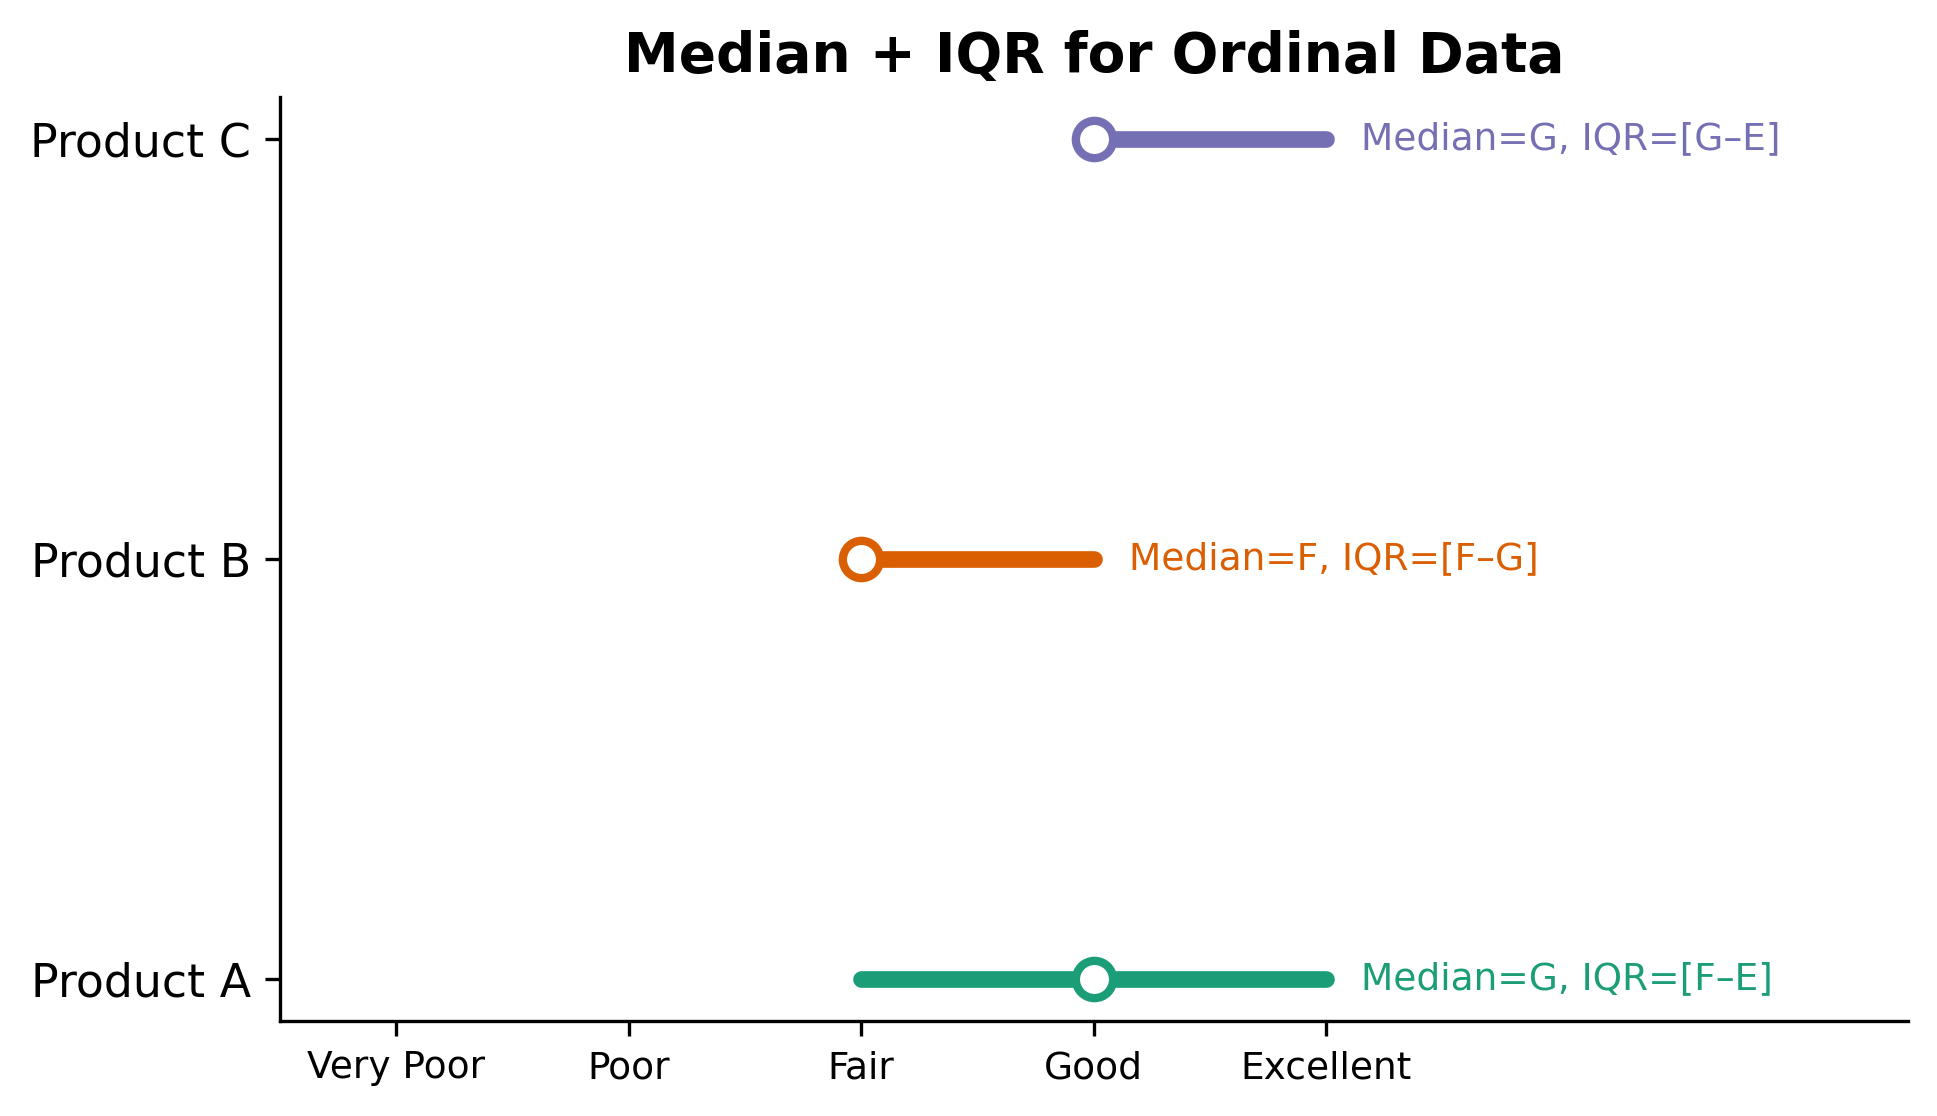
\includegraphics[width=0.72\textwidth]{m3_6_median_iqr.png}

\vspace{0.2cm}
\begin{columns}[T]
\begin{column}{0.48\textwidth}
\begin{itemize}
    \item The \textbf{median} is the correct measure of central tendency for ordinal data
    \item The \textbf{IQR} (Q1--Q3) measures spread
    \item Do \textbf{not} report means for ordinal data in formal work (the ``$3.7 \pm 0.8$ on a 5-point scale'' convention is common but technically improper)
\end{itemize}
\end{column}
\begin{column}{0.48\textwidth}
\begin{alertblock}{Pro-Tip}
    \scriptsize Display the median as a point on the ordinal axis, with a thick bar spanning Q1--Q3. This is the ordinal analog of the pointrange (Module 2.1). Annotate with the actual level names, not just numbers.
\end{alertblock}
\end{column}
\end{columns}
\end{frame}

% ── 161 ──
\begin{frame}[fragile]{Median + IQR --- Code}\smark{161/300}
\begin{columns}[T]
\begin{column}{0.48\textwidth}
\begin{lstlisting}[style=Rstyle]
# Compute ordinal summaries
summ <- df |>
  group_by(product) |>
  summarise(
    med = median(as.numeric(rating)),
    q25 = quantile(as.numeric(rating),
                   0.25),
    q75 = quantile(as.numeric(rating),
                   0.75))

ggplot(summ, aes(y=product)) +
  geom_segment(aes(
    x=q25, xend=q75, yend=product),
    linewidth=4, color="#2166AC",
    lineend="round") +
  geom_point(aes(x=med),
    size=5, color="white",
    stroke=2) +
  scale_x_continuous(
    breaks=1:5, labels=levels)
\end{lstlisting}
\end{column}
\begin{column}{0.48\textwidth}
\begin{lstlisting}[style=Pystyle]
for i, (data, label, c) in enumerate(
    zip(all_data, products, colors)):
    med = np.median(data)
    q25, q75 = np.percentile(
        data, [25, 75])
    ax.plot([q25, q75], [i, i],
        color=c, linewidth=4,
        solid_capstyle="round")
    ax.scatter(med, i,
        color="white", s=80,
        zorder=5, edgecolors=c,
        linewidths=2)
ax.set_xticks(range(5))
ax.set_xticklabels(levels)
ax.set_yticks(range(len(products)))
ax.set_yticklabels(products)
\end{lstlisting}
\end{column}
\end{columns}
\end{frame}

% ── 162 ──
\begin{frame}{Ridgeline for Ordinal Distributions}
\smark{162/300}
\centering
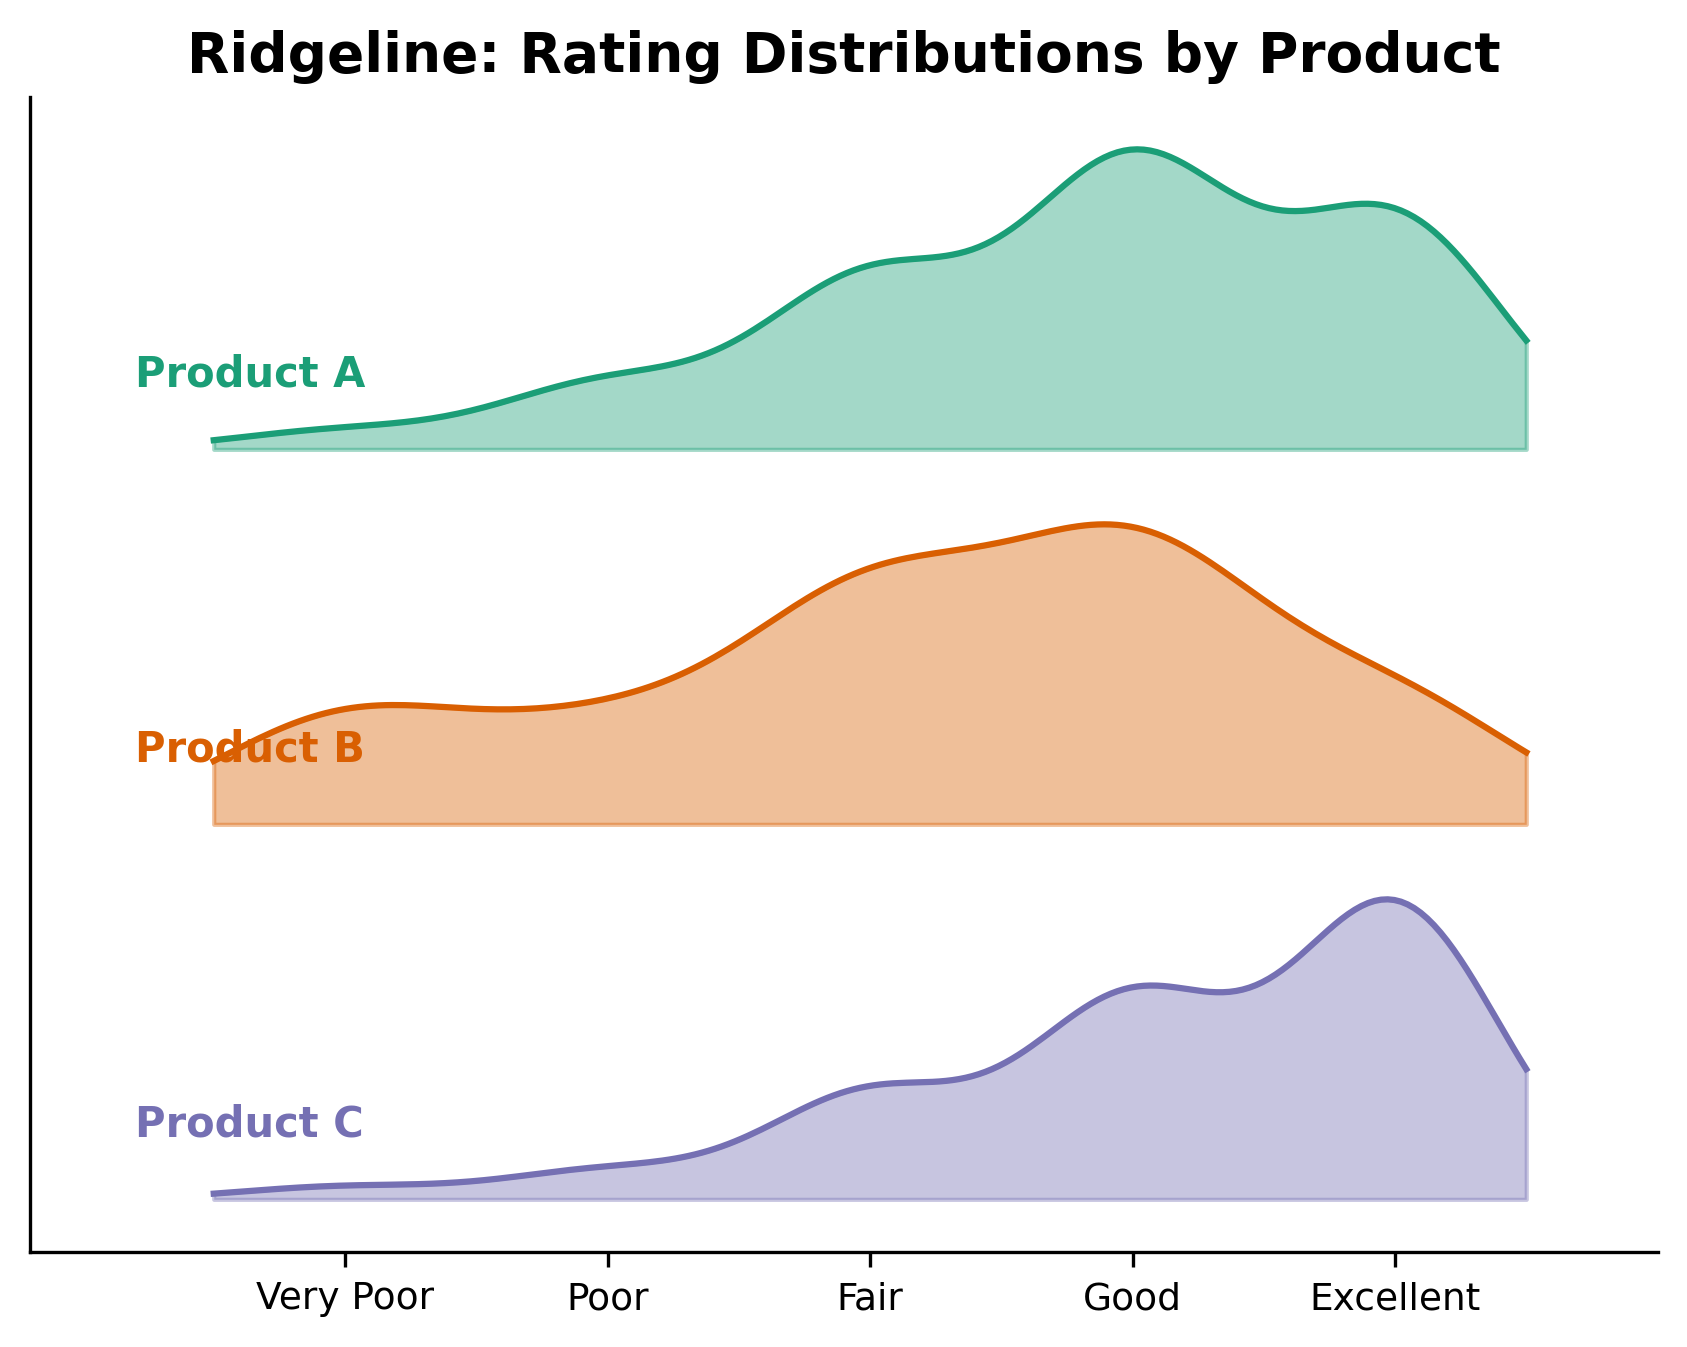
\includegraphics[width=0.62\textwidth]{m3_6_ridgeline_ordinal.png}

\vspace{0.2cm}
\begin{columns}[T]
\begin{column}{0.48\textwidth}
\begin{itemize}
    \item KDE smoothed over the ordinal levels (treated as numeric)
    \item Shows distribution shape per group
    \item Useful when comparing 5+ products on the same scale
    \item The trade-off: smoothing blurs discrete levels
\end{itemize}
\end{column}
\begin{column}{0.48\textwidth}
\begin{alertblock}{Pro-Tip}
    \scriptsize Using KDE on ordinal data is technically treating it as continuous. For purists: use frequency bar charts per level. For pragmatists: KDE with small bandwidth reveals shape patterns that bars cannot. Always label the ordinal levels on the $x$-axis.
\end{alertblock}
\end{column}
\end{columns}
\end{frame}

% ── 163 ──
\begin{frame}[fragile]{Ordinal Ridgeline --- Code}\smark{163/300}
\begin{columns}[T]
\begin{column}{0.48\textwidth}
\begin{lstlisting}[style=Rstyle]
library(ggridges)

# Treat rating as numeric for KDE
df$rating_num <- as.numeric(
  df$rating)

ggplot(df,
  aes(rating_num, product,
      fill = product)) +
  geom_density_ridges(
    alpha = 0.4, scale = 1.2,
    bandwidth = 0.4) +
  scale_x_continuous(
    breaks = 1:5,
    labels = levels) +
  theme_minimal() +
  theme(legend.position="none")
\end{lstlisting}
\end{column}
\begin{column}{0.48\textwidth}
\begin{lstlisting}[style=Pystyle]
from scipy.stats import gaussian_kde

offset = 0
for data, label, c in zip(
    all_data, products, colors):
    kde = gaussian_kde(data,
        bw_method=0.4)
    xs = np.linspace(-0.5, 4.5, 200)
    dens = kde(xs)
    dens = dens/dens.max() * 1.2
    ax.fill_between(xs, offset,
        offset+dens,
        color=c, alpha=0.4)
    ax.plot(xs, offset+dens,
        color=c, linewidth=1.5)
    offset += 1.5
ax.set_xticks(range(5))
ax.set_xticklabels(levels)
\end{lstlisting}
\end{column}
\end{columns}
\end{frame}

% ── 164 ──
\begin{frame}{Proportional Dot Matrix (Icon Array)}
\smark{164/300}
\centering
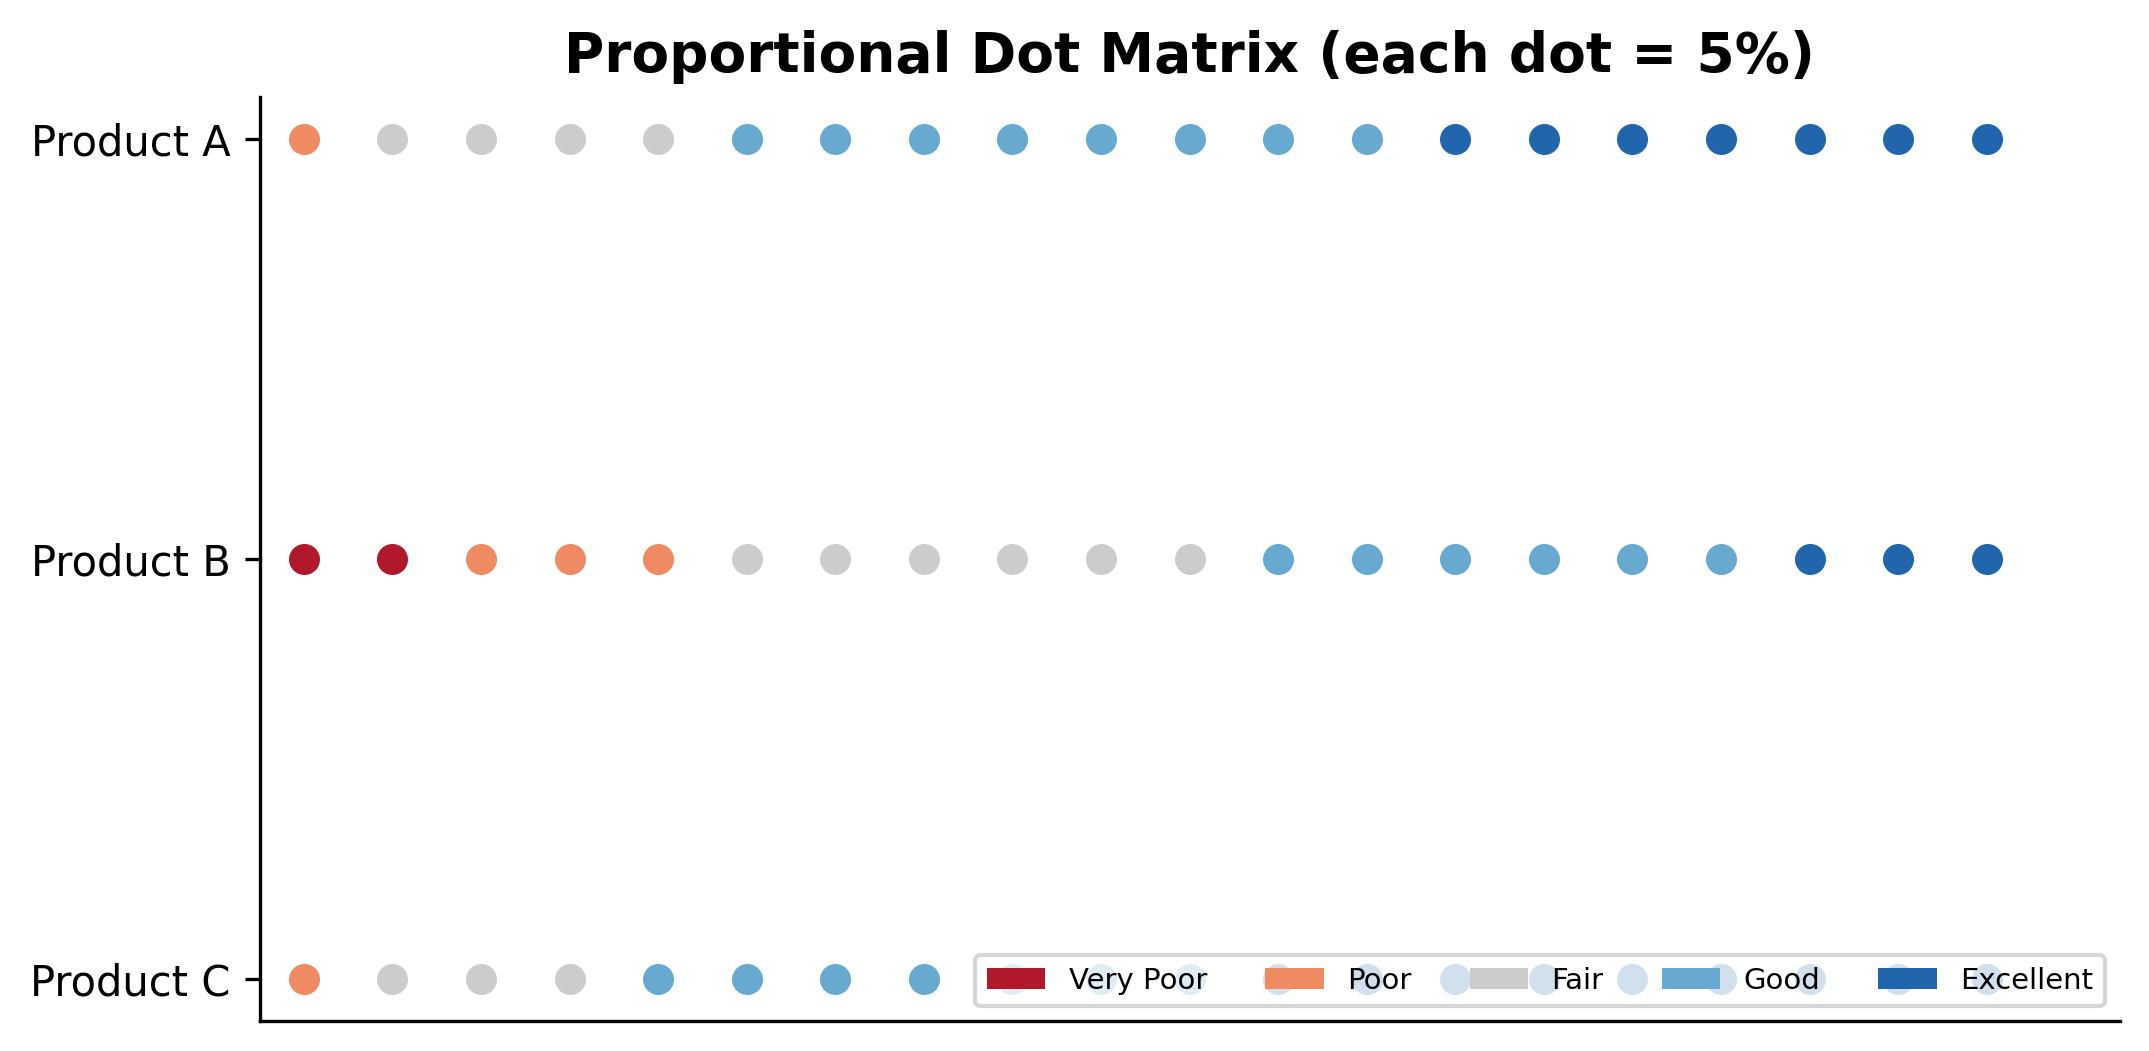
\includegraphics[width=0.72\textwidth]{m3_6_dot_matrix.png}

\vspace{0.2cm}
\begin{columns}[T]
\begin{column}{0.48\textwidth}
\begin{itemize}
    \item Each dot represents a fixed proportion (e.g., 5\%)
    \item Colored by ordinal level
    \item The row of dots acts as a discrete stacked bar
    \item Countable: readers can see ``4 of 20 dots are red''
    \item The waffle chart principle applied per-item
\end{itemize}
\end{column}
\begin{column}{0.48\textwidth}
\begin{exampleblock}{Data Insight}
    \scriptsize Product B has the most red/orange dots (negative ratings) while Product C has the most blue dots (positive). The dot format makes proportional differences more tangible than color areas --- each dot is a countable unit.
\end{exampleblock}
\end{column}
\end{columns}
\end{frame}

% ── 165 ──
\begin{frame}[fragile]{Dot Matrix --- Code}\smark{165/300}
\begin{columns}[T]
\begin{column}{0.48\textwidth}
\begin{lstlisting}[style=Rstyle]
# waffle package can do per-row
library(waffle)
# Or manual with geom_point
df_dots <- expand.grid(
  product = products,
  dot = 1:20) |>
  left_join(level_assignments)

ggplot(df_dots,
  aes(dot, product,
      color = level)) +
  geom_point(size = 3) +
  scale_color_manual(
    values = colors_ord) +
  theme_minimal() +
  theme(panel.grid = element_blank())
\end{lstlisting}
\end{column}
\begin{column}{0.48\textwidth}
\begin{lstlisting}[style=Pystyle]
# Manual dot matrix
for pi, (prod, probs) in enumerate(
    zip(products, all_probs)):
    counts = (np.array(probs)*20)\
        .astype(int)
    counts[-1] = 20 - counts[:-1].sum()
    x = 0
    for li, (cnt, c) in enumerate(
        zip(counts, colors_ord)):
        for _ in range(cnt):
            ax.scatter(x, pi,
                s=60, color=c,
                edgecolors="white",
                linewidths=0.3)
            x += 1
ax.set_yticks(range(len(products)))
ax.set_yticklabels(products)
\end{lstlisting}
\end{column}
\end{columns}
\end{frame}

% ── 166 ──
\begin{frame}{Cumulative Odds and Proportional Odds}
\smark{166/300}
\centering
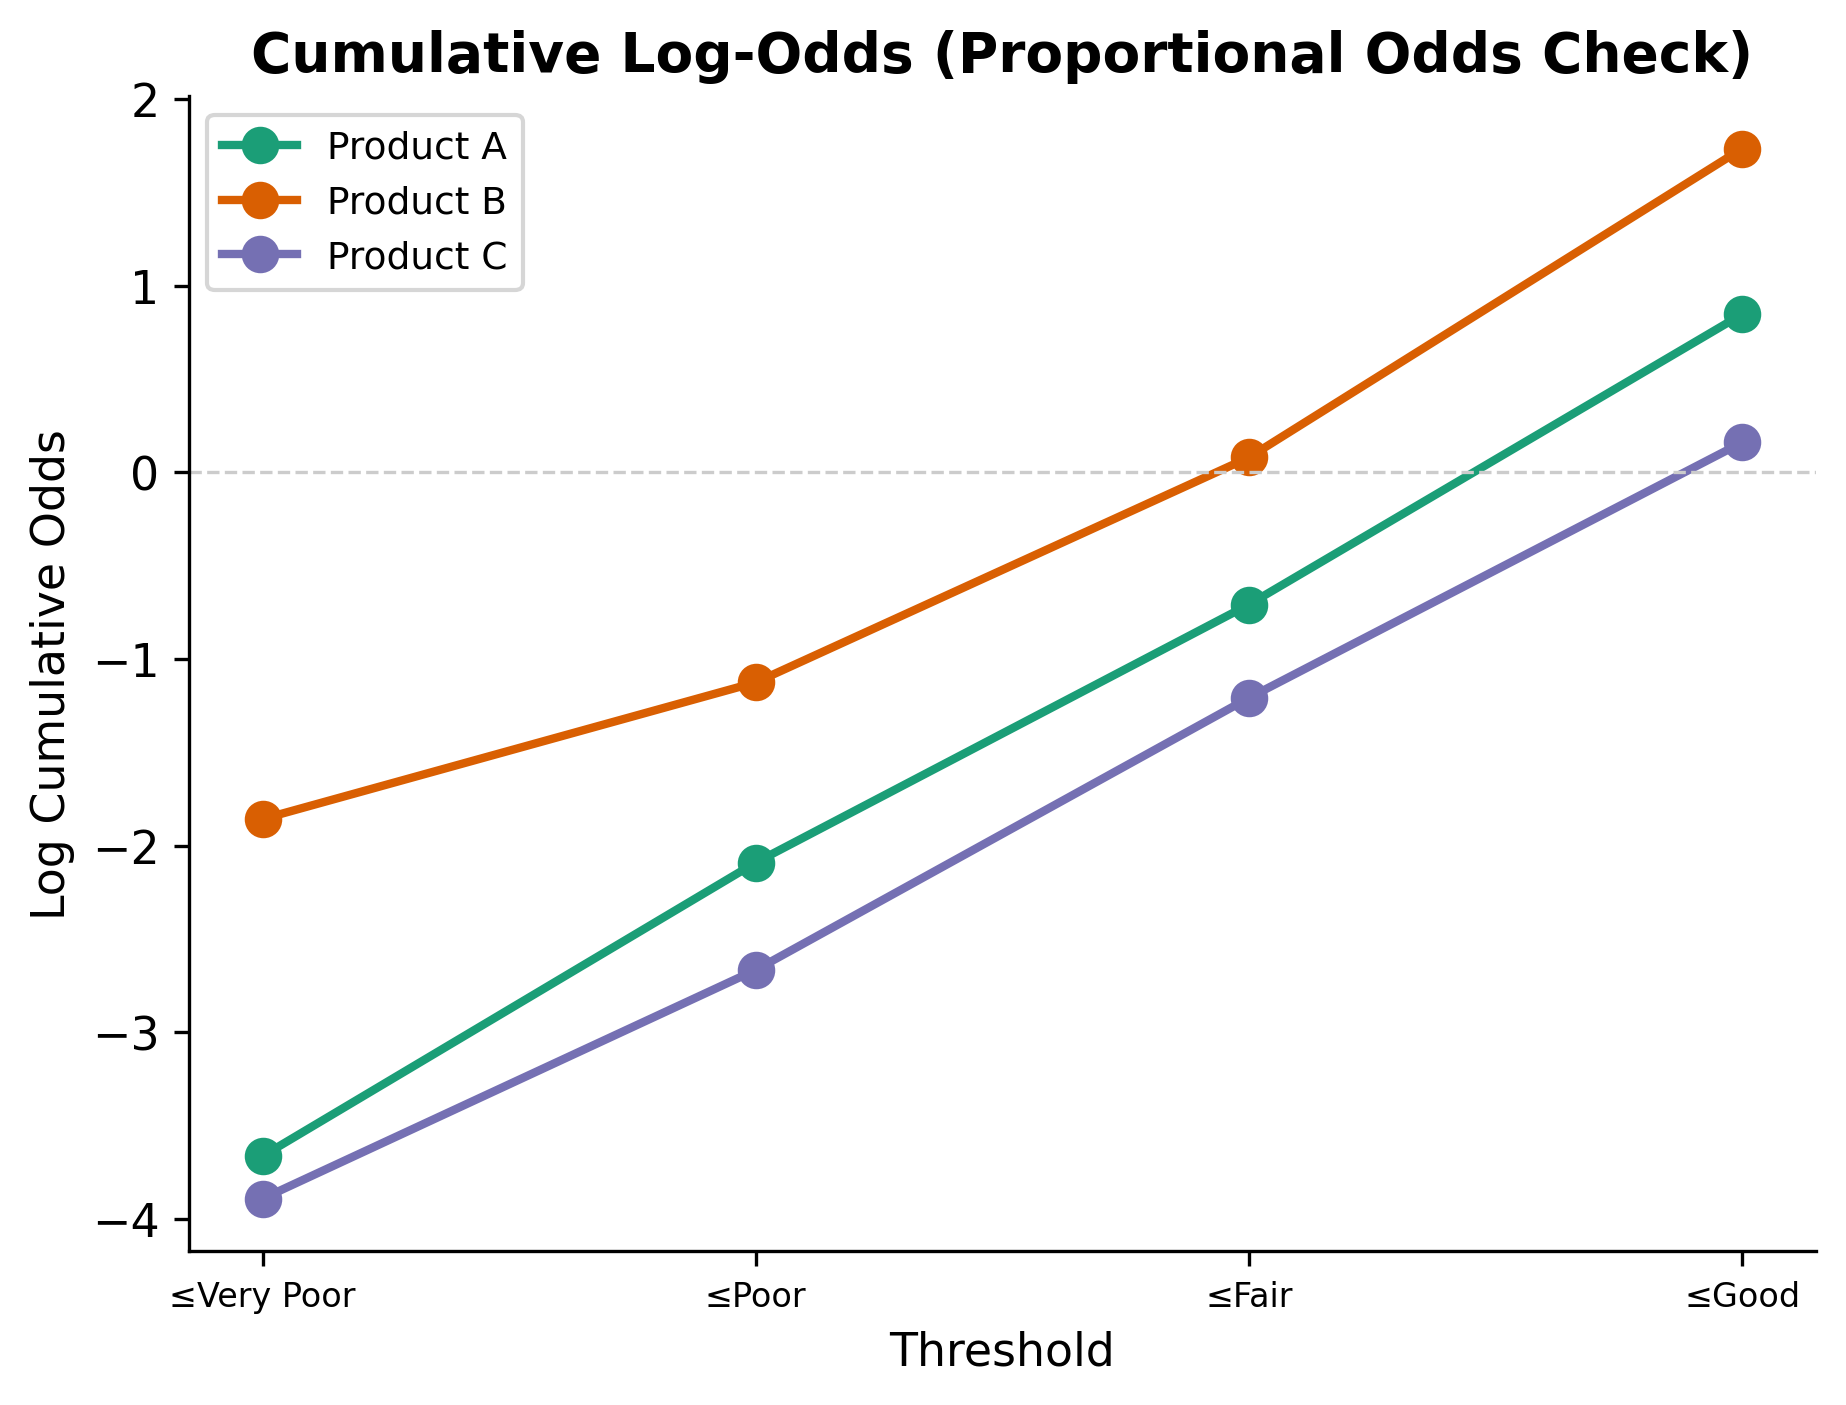
\includegraphics[width=0.65\textwidth]{m3_6_cum_odds.png}

\vspace{0.2cm}
\begin{columns}[T]
\begin{column}{0.48\textwidth}
\begin{itemize}
    \item Cumulative odds: $P(Y \leq j) / P(Y > j)$ at each threshold
    \item Log cumulative odds = logit of the CDF
    \item \textbf{Proportional odds assumption}: curves are \textbf{parallel} (constant shift)
    \item If parallel: ordinal logistic regression is appropriate
\end{itemize}
\end{column}
\begin{column}{0.48\textwidth}
\begin{exampleblock}{Data Insight}
    \scriptsize If the lines are approximately parallel, the proportional odds model fits --- the effect of ``product'' is the same regardless of which threshold you examine. Non-parallel lines mean the effect differs by threshold, requiring a more complex model.
\end{exampleblock}
\end{column}
\end{columns}
\end{frame}

% ── 167 ──
\begin{frame}[fragile]{Proportional Odds Check --- Code}\smark{167/300}
\begin{columns}[T]
\begin{column}{0.48\textwidth}
\begin{lstlisting}[style=Rstyle]
library(MASS)
library(VGAM)

# Fit proportional odds model
model <- polr(rating ~ product,
  data = df, Hess = TRUE)
summary(model)

# Brant test for parallel lines
library(brant)
brant(model)
# Non-significant = PO holds

# Predicted cumulative probs
predict(model, type="probs")
\end{lstlisting}
\end{column}
\begin{column}{0.48\textwidth}
\begin{lstlisting}[style=Pystyle]
from statsmodels.miscmodels\
    .ordinal_model import OrderedModel

model = OrderedModel(y, X,
    distr="logit")
result = model.fit(method="bfgs")
print(result.summary())

# Manual cumulative odds plot
for grp in groups:
    sub = df[df["group"]==grp]
    counts = sub["rating"]\
        .value_counts().sort_index()
    cum = counts.cumsum() / counts.sum()
    odds = cum[:-1] / (1-cum[:-1])
    ax.plot(range(len(odds)),
        np.log(odds), "o-", label=grp)
\end{lstlisting}
\end{column}
\end{columns}
\end{frame}

% ── 168 ──
\begin{frame}{Heat Strips: Multi-Item Ordinal Profiles}
\smark{168/300}
\centering
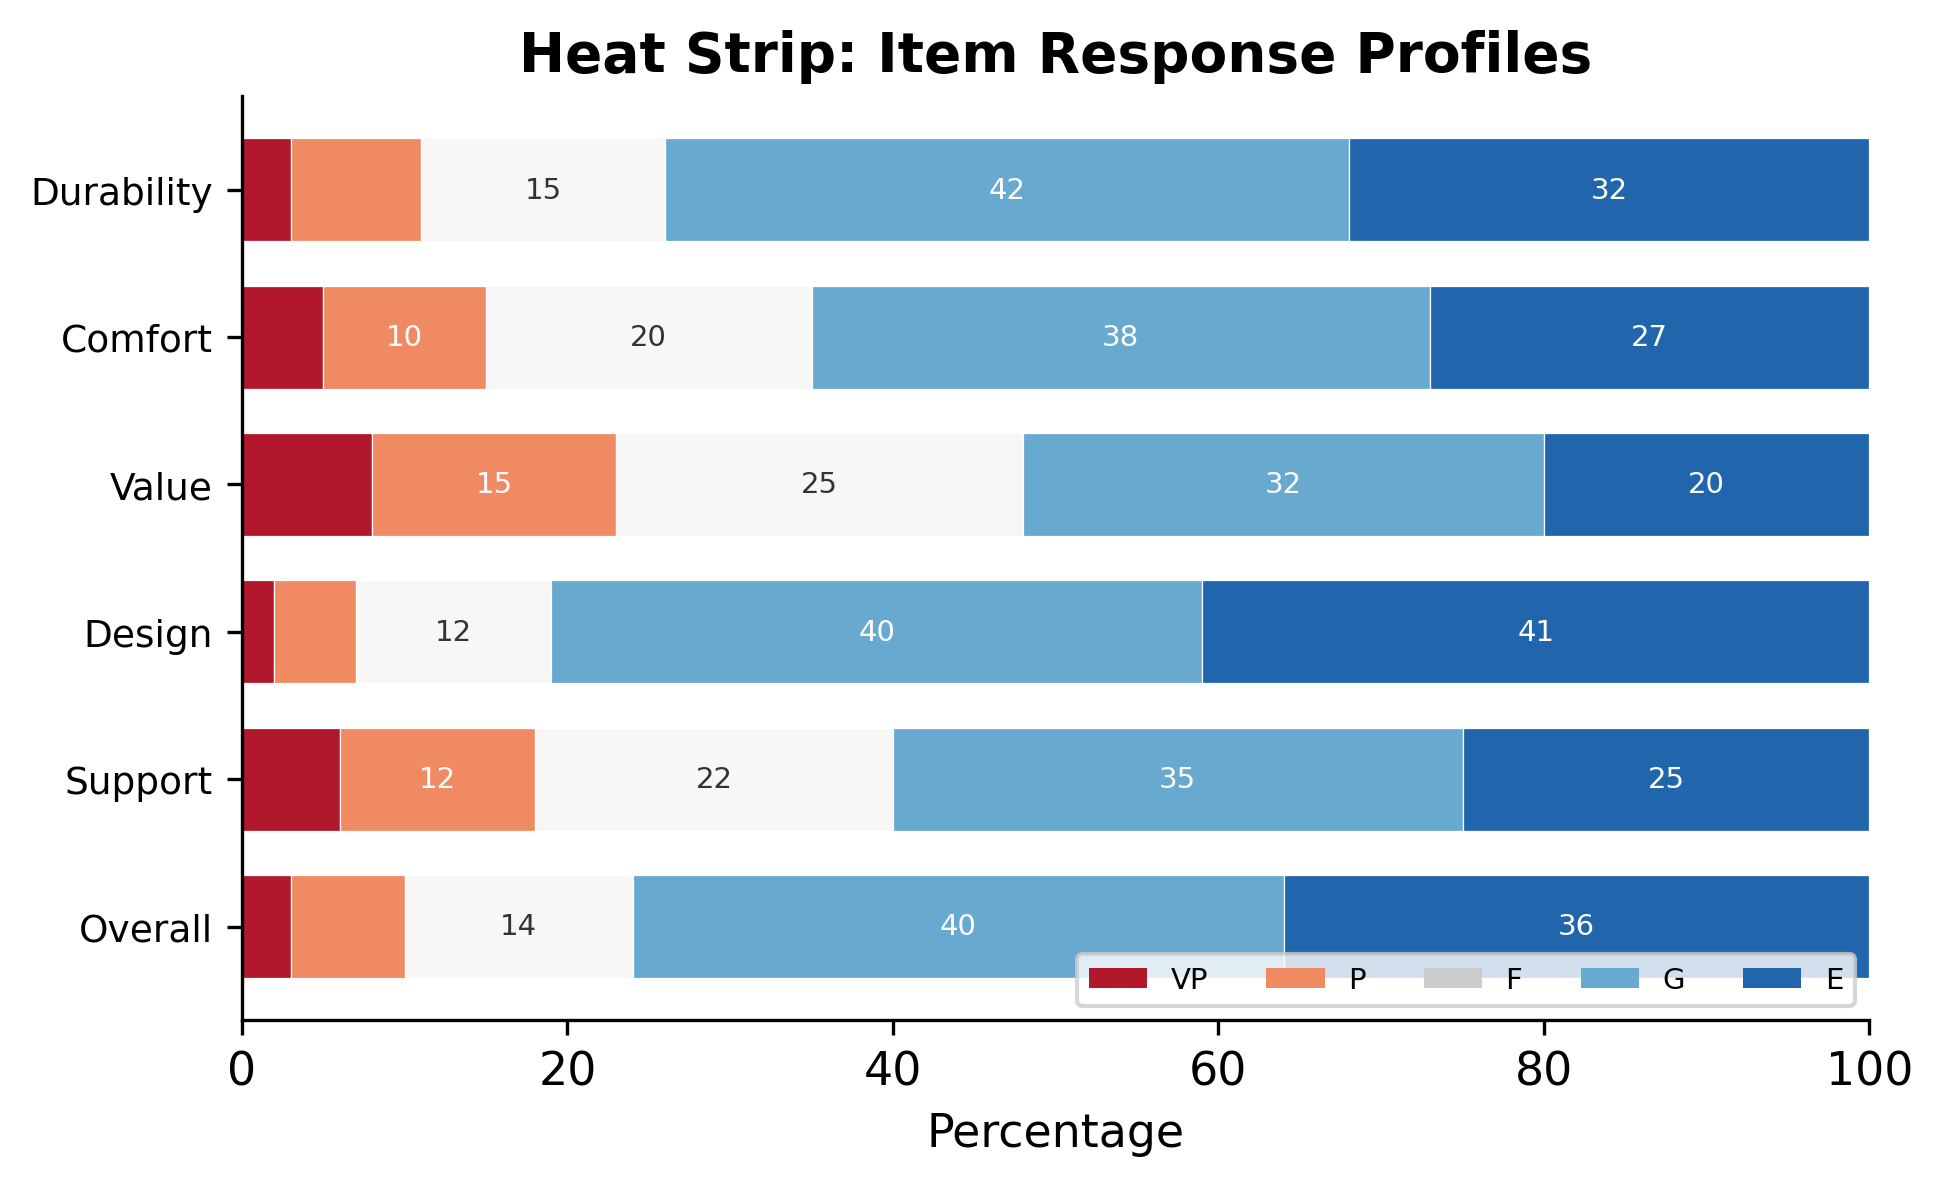
\includegraphics[width=0.72\textwidth]{m3_6_heat_strip.png}

\vspace{0.2cm}
\begin{columns}[T]
\begin{column}{0.48\textwidth}
\begin{itemize}
    \item Each row = one item (question, attribute)
    \item Segments colored by ordinal level
    \item Width $\propto$ percentage in each level
    \item The ``standard stacked bar'' applied to ordinal ratings
    \item Compact: fits 20+ items in one display
\end{itemize}
\end{column}
\begin{column}{0.48\textwidth}
\begin{exampleblock}{Data Insight}
    \scriptsize ``Design'' has the most blue (Excellent). ``Value'' has the most red (Very Poor/Poor). The heat strip scans 6 items in one glance --- faster than reading 6 separate charts.
\end{exampleblock}
\end{column}
\end{columns}
\end{frame}

% ── 169 ──
\begin{frame}[fragile]{Heat Strip --- Code}\smark{169/300}
\begin{columns}[T]
\begin{column}{0.48\textwidth}
\begin{lstlisting}[style=Rstyle]
# Likert package handles this
library(likert)

items <- data.frame(
  Durability=factor(d1, levels=lvls),
  Comfort=factor(d2, levels=lvls),
  Value=factor(d3, levels=lvls))
lik <- likert(items)

# Standard (non-centered) plot
plot(lik, centered=FALSE,
  plot.percents=TRUE)

# Or centered (diverging)
plot(lik, centered=TRUE)
\end{lstlisting}
\end{column}
\begin{column}{0.48\textwidth}
\begin{lstlisting}[style=Pystyle]
# Manual stacked bars
for qi in range(n_items):
    x_start = 0
    for li, c in enumerate(colors_ord):
        val = item_data[qi, li]
        ax.barh(n_items-1-qi, val,
            left=x_start, height=0.7,
            color=c, edgecolor="white",
            linewidth=0.3)
        x_start += val
ax.set_yticks(range(n_items))
ax.set_yticklabels(items[::-1])
ax.set_xlabel("Percentage")
ax.set_xlim(0, 100)
\end{lstlisting}
\end{column}
\end{columns}
\end{frame}

% ── 170 ──
\begin{frame}{Ordinal Tests: Which to Use}
\smark{170/300}
\centering\small
\begin{tabular}{@{}llll@{}}
    \toprule
    \textbf{Comparison} & \textbf{Test} & \textbf{R} & \textbf{Python} \\
    \midrule
    2 groups         & Mann--Whitney $U$         & \texttt{wilcox.test()}        & \texttt{scipy.stats.mannwhitneyu()} \\
    2 paired groups  & Wilcoxon signed-rank      & \texttt{wilcox.test(paired=T)} & \texttt{scipy.stats.wilcoxon()} \\
    3+ groups        & Kruskal--Wallis           & \texttt{kruskal.test()}       & \texttt{scipy.stats.kruskal()} \\
    Post-hoc pairs   & Dunn's test               & \texttt{dunn.test::dunn.test()} & \texttt{scikit-posthocs} \\
    Ordinal regression& Proportional odds        & \texttt{MASS::polr()}         & \texttt{statsmodels.OrderedModel()} \\
    Association       & Spearman $\rho$, Kendall $\tau$ & \texttt{cor.test(method=)} & \texttt{scipy.stats.spearmanr()} \\
    CDF comparison    & KS test                  & \texttt{ks.test()}            & \texttt{scipy.stats.ks\_2samp()} \\
    \bottomrule
\end{tabular}

\vspace{0.2cm}
\begin{alertblock}{Pro-Tip}
    \scriptsize All these tests can be visualized: Mann--Whitney via estimation plots (Module 2.7); Kruskal--Wallis via strip + pairwise Dunn brackets; KS via overlaid cumulative CDFs with max difference annotated.
\end{alertblock}
\end{frame}

% ── 171 ──
\begin{frame}{Star Ratings and Review Data}
\smark{171/300}
\begin{columns}[T]
\begin{column}{0.50\textwidth}
\begin{itemize}
    \item Star ratings (1--5) are ordinal
    \item Common distribution: J-shaped (many 5s and 1s, few 3s)
    \item Mean star rating hides bimodality (``love it or hate it'')
    \item Visualize with: histogram of ratings, diverging stacked bar, or cumulative CDF
\end{itemize}
\end{column}
\begin{column}{0.47\textwidth}
\begin{exampleblock}{Data Insight}
    \scriptsize Amazon, Yelp, and app store ratings are typically bimodal: 5-star and 1-star peaks with a valley at 3. The mean rating (e.g., 3.8) obscures this polarization. A histogram or stacked bar reveals the J-shape immediately.
\end{exampleblock}
\vspace{0.1cm}
\begin{alertblock}{Pro-Tip}
    \scriptsize For review data, show the full star distribution alongside the mean. The ``Rotten Tomatoes'' approach (audience vs.\ critic score) is a net-score variant: percent $\geq 3.5$ stars.
\end{alertblock}
\end{column}
\end{columns}
\end{frame}

% ── 172 ──
\begin{frame}[fragile]{Star Rating Distribution --- Code}\smark{172/300}
\begin{columns}[T]
\begin{column}{0.48\textwidth}
\begin{lstlisting}[style=Rstyle]
# Bar chart of star counts
ggplot(reviews, aes(stars,
    fill=factor(stars))) +
  geom_bar() +
  scale_fill_manual(
    values=c("#B2182B","#EF8A62",
      "#F7F7F7","#67A9CF",
      "#2166AC")) +
  theme_minimal() +
  theme(legend.position="none")

# Horizontal summary
ggplot(reviews,
  aes(x=1, fill=factor(stars))) +
  geom_bar(position="fill",
    width=0.5) +
  coord_flip() + theme_void()
\end{lstlisting}
\end{column}
\begin{column}{0.48\textwidth}
\begin{lstlisting}[style=Pystyle]
counts = reviews["stars"]\
    .value_counts().sort_index()
colors_stars = ["#B2182B","#EF8A62",
    "#F7F7F7","#67A9CF","#2166AC"]

ax.bar(range(1, 6), counts.values,
    color=colors_stars,
    edgecolor="white")
ax.set_xlabel("Star Rating")
ax.set_ylabel("Count")

# Annotate mean
mean_r = reviews["stars"].mean()
ax.axvline(mean_r, color="#333",
    linestyle="--", linewidth=1.5)
ax.text(mean_r+0.1, max(counts)*0.9,
    f"Mean = {mean_r:.1f}",
    fontweight="bold")
\end{lstlisting}
\end{column}
\end{columns}
\end{frame}

% ── 173 ──
\begin{frame}{Agreement Indices: Beyond the Mean}
\smark{173/300}
\begin{columns}[T]
\begin{column}{0.50\textwidth}
\begin{itemize}
    \item \textbf{Consensus index} ($C_n$): measures within-group agreement (0 = full disagreement, 1 = perfect consensus)
    \item \textbf{Interrater reliability}: Cohen's $\kappa$ (2 raters), Fleiss' $\kappa$ (3+ raters), Krippendorff's $\alpha$
    \item \textbf{Entropy}: Shannon entropy of the response distribution (low = concentrated, high = dispersed)
    \item Visualize: plot the agreement index alongside the diverging bar for each item
\end{itemize}
\end{column}
\begin{column}{0.47\textwidth}
\begin{alertblock}{Pro-Tip}
    \scriptsize R: \texttt{irr::kappa2()} for Cohen's $\kappa$; \texttt{irr::kappam.fleiss()} for Fleiss'. Python: \texttt{sklearn.metrics.cohen\_kappa\_score()} for 2 raters; \texttt{krippendorff} package for Krippendorff's $\alpha$.
\end{alertblock}
\end{column}
\end{columns}
\end{frame}

% ── 174 ──
\begin{frame}{Ordinal Effect Sizes}
\smark{174/300}
\centering\small
\begin{tabular}{@{}llll@{}}
    \toprule
    \textbf{Measure} & \textbf{Range} & \textbf{Use} & \textbf{R / Python} \\
    \midrule
    Common language ES & $[0, 1]$  & $P(\text{A} > \text{B})$  & \texttt{effectsize::cles()} / manual \\
    Cliff's $\delta$   & $[-1, 1]$ & Non-parametric $d$       & \texttt{effectsize::cliffs\_delta()} / \texttt{pg.} \\
    Vargha-Delaney $A$ & $[0, 1]$  & Same as CLES             & \texttt{rstatix::wilcox\_effsize()} \\
    Rank-biserial $r$  & $[-1, 1]$ & From Mann--Whitney       & \texttt{wilcox.test()} + manual \\
    Kendall's $W$      & $[0, 1]$  & Multi-rater agreement    & \texttt{irr::kendall()} \\
    \bottomrule
\end{tabular}

\vspace{0.3cm}
\begin{exampleblock}{Data Insight}
    \scriptsize Common Language Effect Size: ``In 73\% of random pairings, a Product C user rates higher than a Product B user.'' This is the most intuitive ordinal effect size --- directly interpretable without statistical training.
\end{exampleblock}
\end{frame}

% ── 175 ──
\begin{frame}[fragile]{Ordinal Effect Sizes --- Code}\smark{175/300}
\begin{columns}[T]
\begin{column}{0.48\textwidth}
\begin{lstlisting}[style=Rstyle]
library(effectsize)

# Cliff's delta
cliffs_delta(rating ~ product,
  data = filter(df,
    product %in% c("A","C")))
# Returns delta + 95% CI

# Common language ES
cles(rating ~ product,
  data = filter(df,
    product %in% c("A","C")))

# Rank-biserial from wilcox
rank_biserial(rating ~ product,
  data = filter(df,
    product %in% c("A","C")))
\end{lstlisting}
\end{column}
\begin{column}{0.48\textwidth}
\begin{lstlisting}[style=Pystyle]
import pingouin as pg

# Cliff's delta
pg.compute_effsize(data_A, data_C,
    eftype="CLES")

# Manual CLES
n_greater = sum(
    a < c for a in data_A
    for c in data_C)
cles = n_greater / (len(data_A) *
    len(data_C))
print(f"CLES = {cles:.3f}")

# Rank-biserial from Mann-Whitney
U, p = stats.mannwhitneyu(
    data_A, data_C)
r = 1 - 2*U / (len(data_A) *
    len(data_C))
\end{lstlisting}
\end{column}
\end{columns}
\end{frame}

% ── 176 ──
\begin{frame}{Ordinal Regression Visualization}
\smark{176/300}
\begin{columns}[T]
\begin{column}{0.50\textwidth}
\begin{itemize}
    \item Proportional odds model: $\text{logit}(P(Y \leq j)) = \alpha_j - \beta X$
    \item Visualize predicted cumulative probabilities per group
    \item \textbf{Effect plot}: predicted $P(Y \leq j)$ across levels of $X$ for each threshold $j$
    \item Coefficient plot with odds ratios (exponentiated $\beta$)
\end{itemize}
\end{column}
\begin{column}{0.47\textwidth}
\begin{alertblock}{Pro-Tip}
    \scriptsize R: \texttt{effects::Effect("product", model)} produces predicted probabilities at each ordinal level. \texttt{sjPlot::plot\_model(model, type="pred")} generates the ggplot2 version. In Python, extract predictions manually from \texttt{OrderedModel}.
\end{alertblock}
\end{column}
\end{columns}
\end{frame}

% ── 177 ──
\begin{frame}[fragile]{Ordinal Regression Viz --- Code}\smark{177/300}
\begin{columns}[T]
\begin{column}{0.48\textwidth}
\begin{lstlisting}[style=Rstyle]
library(MASS)
library(effects)

model <- polr(rating ~ product,
  data = df, Hess = TRUE)

# Predicted probabilities
plot(Effect("product", model),
  style = "stacked",
  colors = colors_ord)

# OR: sjPlot
library(sjPlot)
plot_model(model, type = "pred",
  terms = "product") +
  theme_minimal()

# Odds ratios + CI
exp(cbind(OR=coef(model),
  confint(model)))
\end{lstlisting}
\end{column}
\begin{column}{0.48\textwidth}
\begin{lstlisting}[style=Pystyle]
from statsmodels.miscmodels\
    .ordinal_model import OrderedModel

model = OrderedModel(y, X,
    distr="logit")
result = model.fit(method="bfgs")

# Predicted probabilities
pred = result.predict()
# Returns matrix: n x K levels

# Plot stacked predicted probs
for product_val in products:
    pred_probs = model.predict(
        X_grid)
    # Stacked bar of predicted
    # probabilities per level
    x_start = 0
    for li, c in enumerate(colors):
        ax.barh(pi, pred_probs[li],
            left=x_start, color=c)
        x_start += pred_probs[li]
\end{lstlisting}
\end{column}
\end{columns}
\end{frame}

% ── 178 ──
\begin{frame}{Ordinal Visualization Decision Guide}
\smark{178/300}
\centering\small
\begin{tabular}{@{}lll@{}}
    \toprule
    \textbf{Task} & \textbf{Plot} & \textbf{Key Feature} \\
    \midrule
    Compare distributions        & Cumulative CDF (step)     & Stochastic dominance \\
    Compare rating profiles      & Diverging stacked bar     & Balance of positive/negative \\
    Summarize center + spread    & Median + IQR pointrange   & Ordinal-safe statistics \\
    Many items at once           & Heat strip                & Compact multi-item view \\
    Shape comparison             & Ridgeline                 & KDE per group \\
    Countable proportions        & Dot matrix                & Each dot = fixed \% \\
    Model check                  & Cumulative log-odds       & Proportional odds assumption \\
    Effect size                  & CLES / Cliff's $\delta$   & Non-parametric magnitude \\
    Predicted probabilities      & Stacked predicted probs   & From ordinal regression \\
    \bottomrule
\end{tabular}
\end{frame}

% ── 179 ──
\begin{frame}{Common Mistakes with Ordinal Data}
\smark{179/300}
\centering\small
\begin{tabular}{@{}ll@{}}
    \toprule
    \textbf{Mistake} & \textbf{Fix} \\
    \midrule
    Sorting ordinal categories by count    & Preserve intrinsic order \\
    Reporting mean $\pm$ SD                & Report median + IQR \\
    Using $t$-test / ANOVA                 & Use Mann--Whitney / Kruskal--Wallis \\
    Treating 5-point scale as continuous   & Use ordinal regression or non-parametric tests \\
    Bar chart without showing distribution & Add diverging stacked or cumulative CDF \\
    Ignoring bimodality in star ratings    & Show full distribution, not just mean \\
    \bottomrule
\end{tabular}
\end{frame}

% ── 180 ──
\begin{frame}{Module 3.6 --- Key Takeaways}\smark{180/300}
\begin{enumerate}
    \item \textbf{Preserve ordinal order.} Never sort by count.
    \item \textbf{Cumulative CDFs} reveal stochastic dominance --- the strongest ordinal comparison.
    \item \textbf{Median + IQR} is the correct summary for ordinal data (not mean $\pm$ SD).
    \item \textbf{Diverging stacked bars} work for ordinal ratings just as for Likert (Module 3.4).
    \item \textbf{Proportional odds check}: plot log cumulative odds --- parallel lines confirm the model.
    \item \textbf{CLES and Cliff's $\delta$} are non-parametric effect sizes for ordinal comparisons.
\end{enumerate}
\end{frame}

% ── 181 ──
\begin{frame}{}\smark{181/300}
\centering\vspace{1.5cm}
{\Large\textbf{Module 3.6 Complete}}\\[0.5cm]
You can now visualize ordinal data with cumulative CDFs, diverging bars, median+IQR, ridgelines, dot matrices, and proportional-odds diagnostics --- using order-respecting methods throughout.\\[0.5cm]
\textbf{Next:} Module 3.7 --- Contingency Table Variants: Log-Linear Models and Fourfold Displays.
\end{frame}

% ═══════════════════════════════════════════════════════
%  MODULE 3.7+ — Append here
% ═══════════════════════════════════════════════════════

\end{document}